% Options for packages loaded elsewhere
\PassOptionsToPackage{unicode}{hyperref}
\PassOptionsToPackage{hyphens}{url}
\PassOptionsToPackage{dvipsnames,svgnames*,x11names*}{xcolor}
%
\documentclass[
]{krantz}
\usepackage{lmodern}
\usepackage{amssymb,amsmath}
\usepackage{ifxetex,ifluatex}
\ifnum 0\ifxetex 1\fi\ifluatex 1\fi=0 % if pdftex
  \usepackage[T1]{fontenc}
  \usepackage[utf8]{inputenc}
  \usepackage{textcomp} % provide euro and other symbols
\else % if luatex or xetex
  \usepackage{unicode-math}
  \defaultfontfeatures{Scale=MatchLowercase}
  \defaultfontfeatures[\rmfamily]{Ligatures=TeX,Scale=1}
\fi
% Use upquote if available, for straight quotes in verbatim environments
\IfFileExists{upquote.sty}{\usepackage{upquote}}{}
\IfFileExists{microtype.sty}{% use microtype if available
  \usepackage[]{microtype}
  \UseMicrotypeSet[protrusion]{basicmath} % disable protrusion for tt fonts
}{}
\makeatletter
\@ifundefined{KOMAClassName}{% if non-KOMA class
  \IfFileExists{parskip.sty}{%
    \usepackage{parskip}
  }{% else
    \setlength{\parindent}{0pt}
    \setlength{\parskip}{6pt plus 2pt minus 1pt}}
}{% if KOMA class
  \KOMAoptions{parskip=half}}
\makeatother
\usepackage{xcolor}
\IfFileExists{xurl.sty}{\usepackage{xurl}}{} % add URL line breaks if available
\IfFileExists{bookmark.sty}{\usepackage{bookmark}}{\usepackage{hyperref}}
\hypersetup{
  pdftitle={GLMs and Multilevel Models},
  pdfauthor={Paul Roback and Julie Legler},
  colorlinks=true,
  linkcolor=Maroon,
  filecolor=Maroon,
  citecolor=Blue,
  urlcolor=Blue,
  pdfcreator={LaTeX via pandoc}}
\urlstyle{same} % disable monospaced font for URLs
\usepackage{color}
\usepackage{fancyvrb}
\newcommand{\VerbBar}{|}
\newcommand{\VERB}{\Verb[commandchars=\\\{\}]}
\DefineVerbatimEnvironment{Highlighting}{Verbatim}{commandchars=\\\{\}}
% Add ',fontsize=\small' for more characters per line
\usepackage{framed}
\definecolor{shadecolor}{RGB}{248,248,248}
\newenvironment{Shaded}{\begin{snugshade}}{\end{snugshade}}
\newcommand{\AlertTok}[1]{\textcolor[rgb]{0.33,0.33,0.33}{#1}}
\newcommand{\AnnotationTok}[1]{\textcolor[rgb]{0.37,0.37,0.37}{\textbf{\textit{#1}}}}
\newcommand{\AttributeTok}[1]{\textcolor[rgb]{0.61,0.61,0.61}{#1}}
\newcommand{\BaseNTok}[1]{\textcolor[rgb]{0.06,0.06,0.06}{#1}}
\newcommand{\BuiltInTok}[1]{#1}
\newcommand{\CharTok}[1]{\textcolor[rgb]{0.5,0.5,0.5}{#1}}
\newcommand{\CommentTok}[1]{\textcolor[rgb]{0.37,0.37,0.37}{\textit{#1}}}
\newcommand{\CommentVarTok}[1]{\textcolor[rgb]{0.37,0.37,0.37}{\textbf{\textit{#1}}}}
\newcommand{\ConstantTok}[1]{\textcolor[rgb]{0,0,0}{#1}}
\newcommand{\ControlFlowTok}[1]{\textcolor[rgb]{0.27,0.27,0.27}{\textbf{#1}}}
\newcommand{\DataTypeTok}[1]{\textcolor[rgb]{0.27,0.27,0.27}{#1}}
\newcommand{\DecValTok}[1]{\textcolor[rgb]{0.06,0.06,0.06}{#1}}
\newcommand{\DocumentationTok}[1]{\textcolor[rgb]{0.37,0.37,0.37}{\textbf{\textit{#1}}}}
\newcommand{\ErrorTok}[1]{\textcolor[rgb]{0.14,0.14,0.14}{\textbf{#1}}}
\newcommand{\ExtensionTok}[1]{#1}
\newcommand{\FloatTok}[1]{\textcolor[rgb]{0.06,0.06,0.06}{#1}}
\newcommand{\FunctionTok}[1]{\textcolor[rgb]{0,0,0}{#1}}
\newcommand{\ImportTok}[1]{#1}
\newcommand{\InformationTok}[1]{\textcolor[rgb]{0.37,0.37,0.37}{\textbf{\textit{#1}}}}
\newcommand{\KeywordTok}[1]{\textcolor[rgb]{0.27,0.27,0.27}{\textbf{#1}}}
\newcommand{\NormalTok}[1]{#1}
\newcommand{\OperatorTok}[1]{\textcolor[rgb]{0.43,0.43,0.43}{\textbf{#1}}}
\newcommand{\OtherTok}[1]{\textcolor[rgb]{0.37,0.37,0.37}{#1}}
\newcommand{\PreprocessorTok}[1]{\textcolor[rgb]{0.37,0.37,0.37}{\textit{#1}}}
\newcommand{\RegionMarkerTok}[1]{#1}
\newcommand{\SpecialCharTok}[1]{\textcolor[rgb]{0,0,0}{#1}}
\newcommand{\SpecialStringTok}[1]{\textcolor[rgb]{0.5,0.5,0.5}{#1}}
\newcommand{\StringTok}[1]{\textcolor[rgb]{0.5,0.5,0.5}{#1}}
\newcommand{\VariableTok}[1]{\textcolor[rgb]{0,0,0}{#1}}
\newcommand{\VerbatimStringTok}[1]{\textcolor[rgb]{0.5,0.5,0.5}{#1}}
\newcommand{\WarningTok}[1]{\textcolor[rgb]{0.37,0.37,0.37}{\textbf{\textit{#1}}}}
\usepackage{longtable,booktabs}
% Correct order of tables after \paragraph or \subparagraph
\usepackage{etoolbox}
\makeatletter
\patchcmd\longtable{\par}{\if@noskipsec\mbox{}\fi\par}{}{}
\makeatother
% Allow footnotes in longtable head/foot
\IfFileExists{footnotehyper.sty}{\usepackage{footnotehyper}}{\usepackage{footnote}}
\makesavenoteenv{longtable}
\usepackage{graphicx,grffile}
\makeatletter
\def\maxwidth{\ifdim\Gin@nat@width>\linewidth\linewidth\else\Gin@nat@width\fi}
\def\maxheight{\ifdim\Gin@nat@height>\textheight\textheight\else\Gin@nat@height\fi}
\makeatother
% Scale images if necessary, so that they will not overflow the page
% margins by default, and it is still possible to overwrite the defaults
% using explicit options in \includegraphics[width, height, ...]{}
\setkeys{Gin}{width=\maxwidth,height=\maxheight,keepaspectratio}
% Set default figure placement to htbp
\makeatletter
\def\fps@figure{htbp}
\makeatother
\setlength{\emergencystretch}{3em} % prevent overfull lines
\providecommand{\tightlist}{%
  \setlength{\itemsep}{0pt}\setlength{\parskip}{0pt}}
\setcounter{secnumdepth}{5}
\usepackage{booktabs}
%These packages added to resolve tex problems arising from kable tables.
\usepackage{tabularx}
\usepackage{float}
%%
\usepackage{longtable}
\usepackage[bf,singlelinecheck=off]{caption}

\usepackage{framed,color}
\definecolor{shadecolor}{RGB}{248,248,248}

\renewcommand{\textfraction}{0.05}
\renewcommand{\topfraction}{0.8}
\renewcommand{\bottomfraction}{0.8}
\renewcommand{\floatpagefraction}{0.75}

%%%%%%%%
% Inserting new commands here

%% Chapter 2
\newcommand{\lik}{\mathrm{Lik}}
\newcommand{\Lik}{\mathrm{Lik}}

\newcommand{\bstop}{p_{S|B1}}
\newcommand{\nstop}{p_{S|N}}

\newcommand{\thisismynewcommand}{p_{B|\textrm{B Bias}}}
\newcommand{\neutral}{p_{B|N}}
\newcommand{\gbias}{p_{B|\textrm{G Bias}}}
\newcommand{\bbias}{p_{B|\textrm{B Bias}}}

%% Chapter 3
\newcommand{\E}{\operatorname{E}}
\newcommand{\SD}{\operatorname{SD}}

%% Chapter 5
\newcommand{\var}{\operatorname{Var}}

%%%%%%%%

\renewenvironment{quote}{\begin{VF}}{\end{VF}}
\let\oldhref\href
\renewcommand{\href}[2]{#2\footnote{\url{#1}}}

\makeatletter
\newenvironment{kframe}{%
\medskip{}
\setlength{\fboxsep}{.8em}
 \def\at@end@of@kframe{}%
 \ifinner\ifhmode%
  \def\at@end@of@kframe{\end{minipage}}%
  \begin{minipage}{\columnwidth}%
 \fi\fi%
 \def\FrameCommand##1{\hskip\@totalleftmargin \hskip-\fboxsep
 \colorbox{shadecolor}{##1}\hskip-\fboxsep
     % There is no \\@totalrightmargin, so:
     \hskip-\linewidth \hskip-\@totalleftmargin \hskip\columnwidth}%
 \MakeFramed {\advance\hsize-\width
   \@totalleftmargin\z@ \linewidth\hsize
   \@setminipage}}%
 {\par\unskip\endMakeFramed%
 \at@end@of@kframe}
\makeatother

% This change to the shaded environment adapted from https://github.com/yihui/bookdown-chinese/commit/a3e392593b464ba31a7eceb0cd60f7e0bd112798 and https://stackoverflow.com/questions/41052687/rstudio-pdf-knit-fails-with-environment-shaded-undefined-error
\makeatletter
\@ifundefined{Shaded}{
}{\renewenvironment{Shaded}{\begin{kframe}}{\end{kframe}}}
\makeatother

\usepackage{makeidx}
\makeindex

\urlstyle{tt}

\usepackage{amsthm}
\makeatletter
\def\thm@space@setup{%
  \thm@preskip=8pt plus 2pt minus 4pt
  \thm@postskip=\thm@preskip
}
\makeatother

\frontmatter
\usepackage[]{natbib}
\bibliographystyle{plainnat}

\title{GLMs and Multilevel Models}
\usepackage{etoolbox}
\makeatletter
\providecommand{\subtitle}[1]{% add subtitle to \maketitle
  \apptocmd{\@title}{\par {\large #1 \par}}{}{}
}
\makeatother
\subtitle{Broadening Your Statistical Horizons with Applications using R}
\author{Paul Roback and Julie Legler}
\date{2020-07-11}

\begin{document}
\maketitle

% you may need to leave a few empty pages before the dedication page

%\cleardoublepage\newpage\thispagestyle{empty}\null
%\cleardoublepage\newpage\thispagestyle{empty}\null
%\cleardoublepage\newpage
\thispagestyle{empty}

\setlength{\abovedisplayskip}{-5pt}
\setlength{\abovedisplayshortskip}{-5pt}

{
\hypersetup{linkcolor=}
\setcounter{tocdepth}{2}
\tableofcontents
}
\mainmatter

\hypertarget{preface}{%
\chapter*{Preface}\label{preface}}


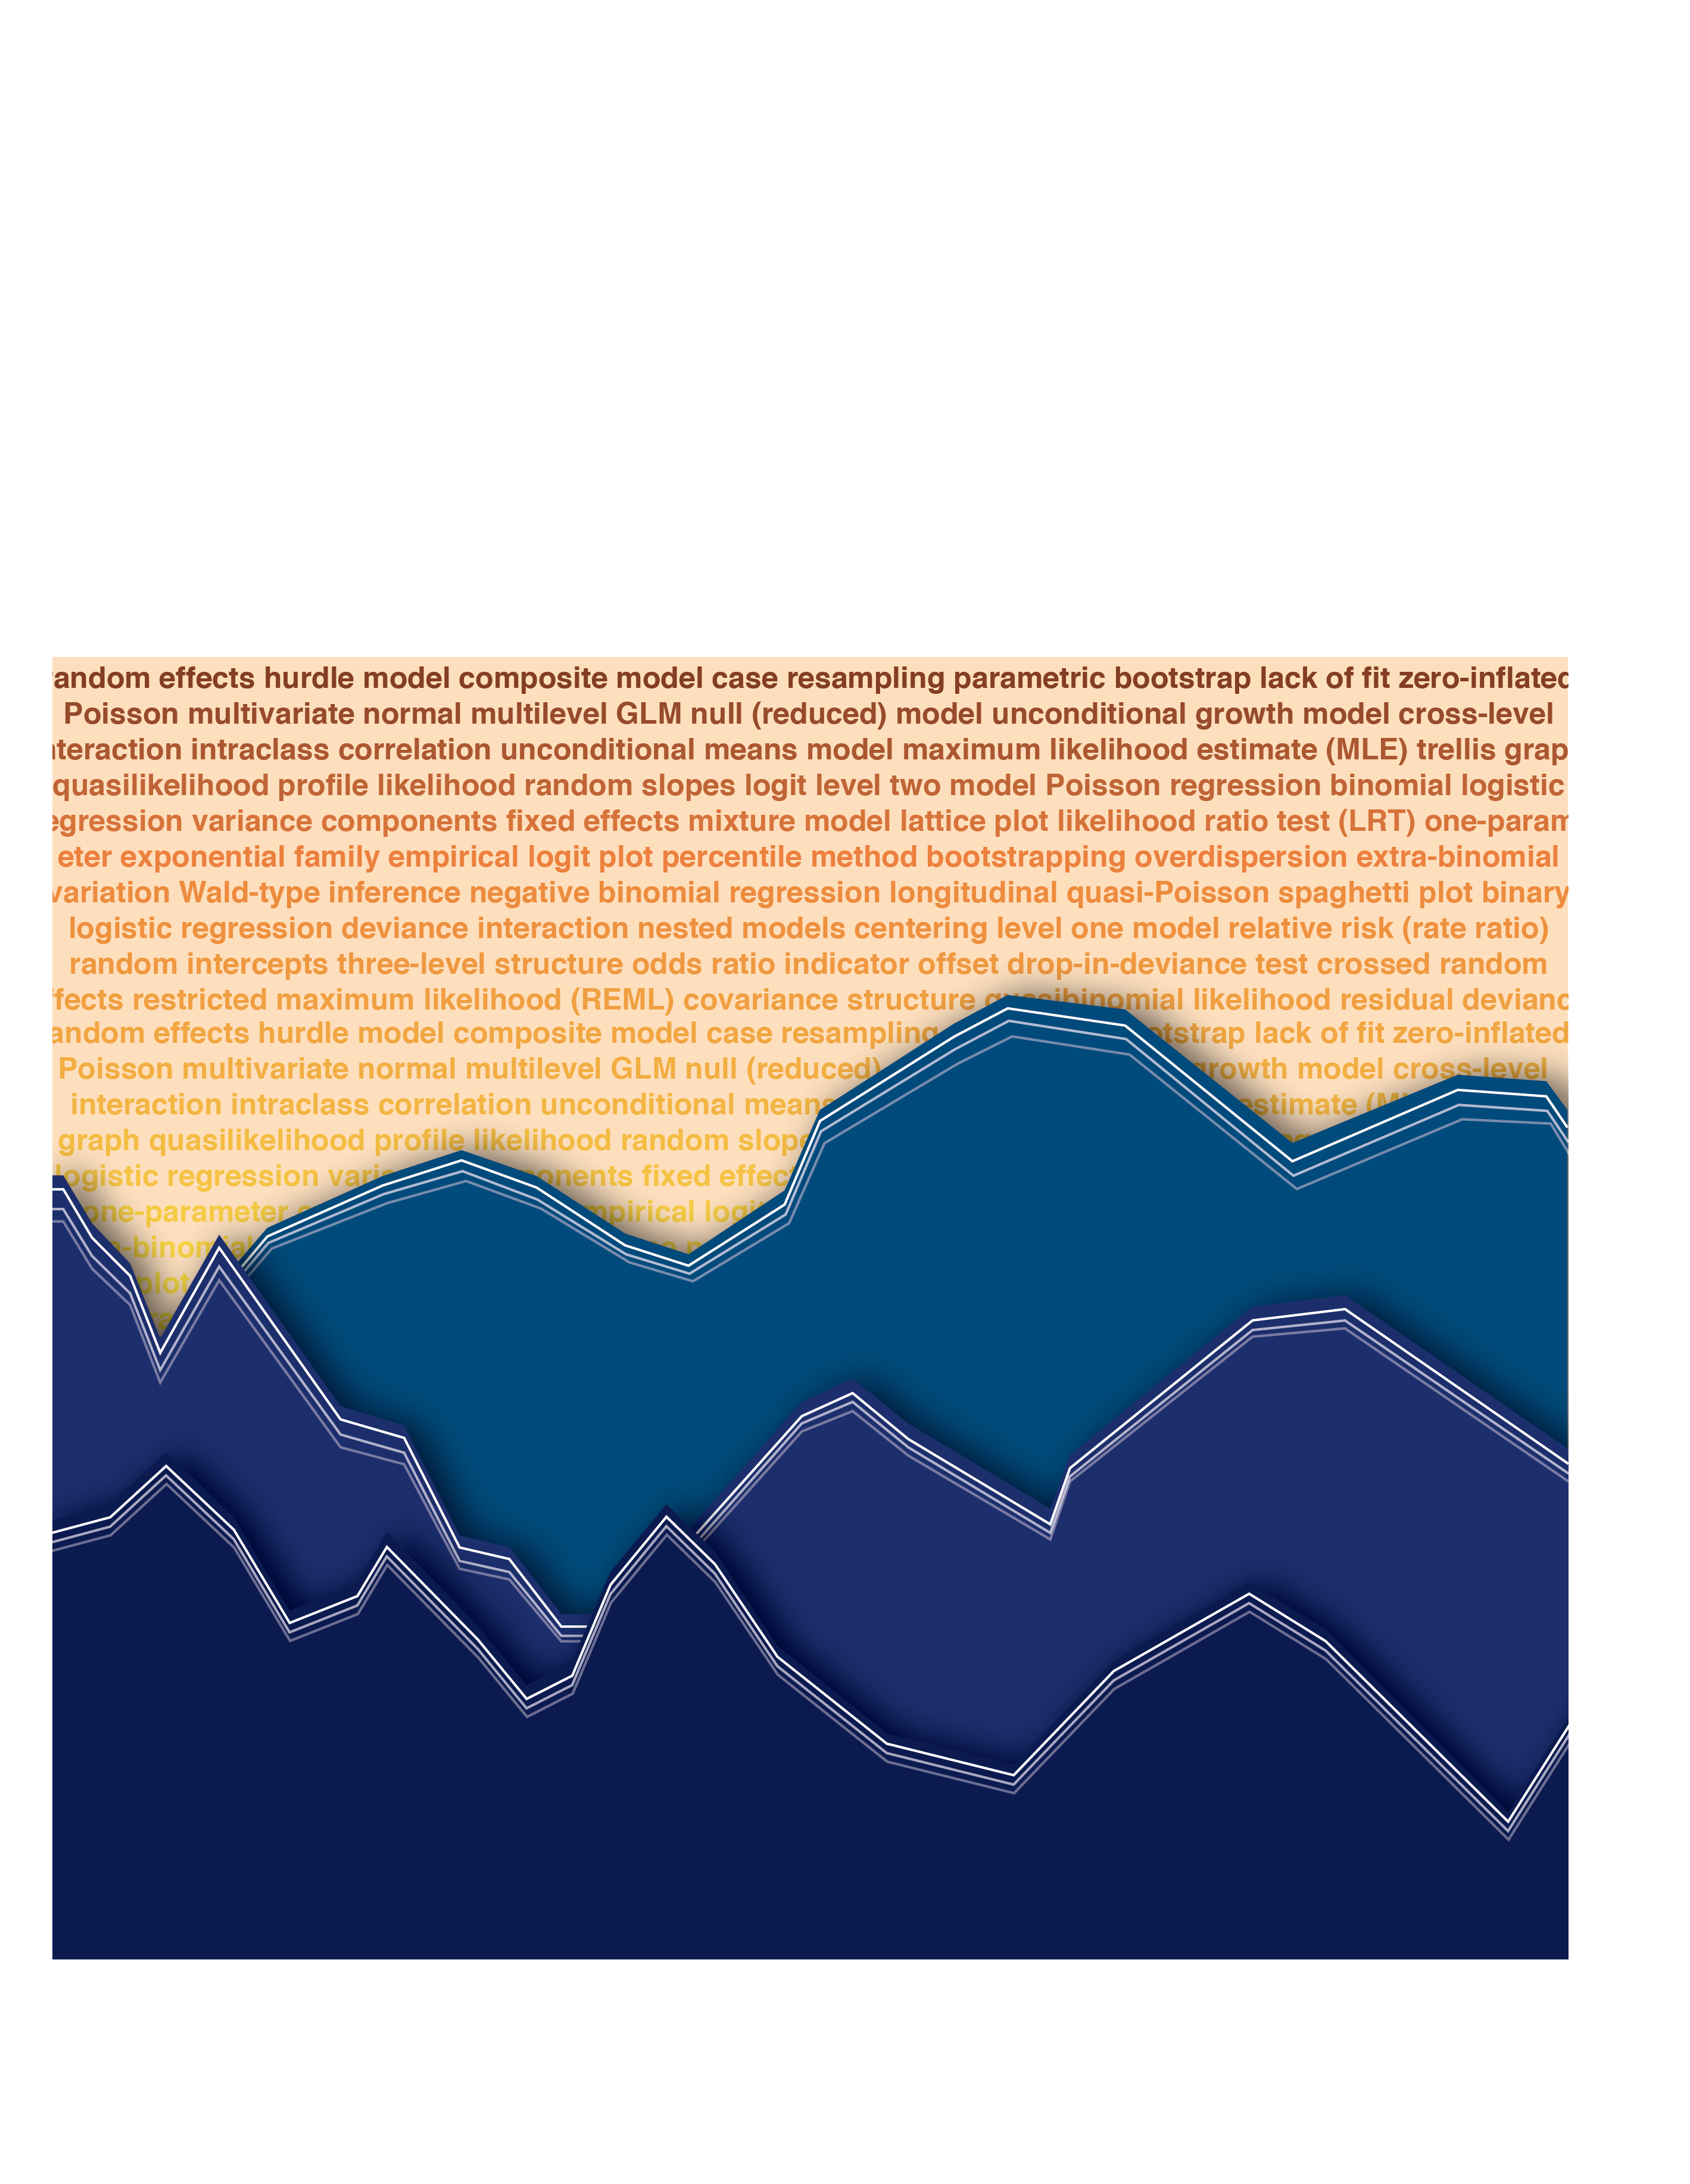
\includegraphics[width=0.75\linewidth]{data/cover}

\textbf{GLMs and Multilevel Models: Broadening Your Statistical Horizons (BYSH) with Applications using R} \citet{RProject} is intended to be accessible to undergraduate students who have successfully completed a regression course through, for example, a textbook like \emph{Stat2} \citep{Cannon2019}. We started teaching this course at St.~Olaf in 2003 so students would be able to deal with the non-normal, correlated world we live in. It has been offered at St.~Olaf every year since. Even though there is no mathematical prerequisite, we still introduce fairly sophisticated topics such as likelihood theory, zero-inflated Poisson, and parametric bootstrapping in an intuitive and applied manner. We believe strongly in case studies featuring real data and real research questions; thus, most of the data in the textbook and \href{https://github.com/proback/BYSH}{available at our GitHub repo} arises from collaborative research conducted by the authors and their students, or from student projects. Our goal is that, after working through this material, students will not necessarily be expert in these methods and associated theory, but that they will develop an expanded toolkit and a greater appreciation for the wider world of data and statistical modeling.

This work is licensed under a Creative Commons Attribution-NonCommercial-ShareAlike 4.0 International License.

\textbf{Acknowledgements.} We would like to thank students of Stat 316 at St.~Olaf College since 2010 for their patience as this book has taken shape with their feedback. We would especially like to thank these St.~Olaf students for their summer research efforts which significantly improved aspects of this book: Cecilia Noecker, Anna Johanson, Nicole Bettes, Kiegan Rice, Anna Wall, Jack Wolf, Josh Pelayo, Spencer Eanes, and Emily Patterson. Early editions of this book also benefitted greatly from feedback from instructors who used these materials in their classes, including Matt Beckman, Laura Boehm Vock, Beth Chance, Laura Chihara, Mine Dogucu, and Katie Ziegler-Graham. Finally, we have appreciated the support of two NSF grants (\#DMS-1045015 and \#DMS-0354308) and of our colleagues in Mathematics, Statistics, and Computer Science at St.~Olaf.

\hypertarget{ch-multilevelintro}{%
\chapter{Introduction to Multilevel Models}\label{ch-multilevelintro}}

\hypertarget{learning-objectives}{%
\section{Learning Objectives}\label{learning-objectives}}

After finishing this chapter, you should be able to:

\begin{itemize}
\tightlist
\item
  Recognize when response variables and covariates have been collected at multiple (nested) levels.
\item
  Apply exploratory data analysis techniques to multilevel data.
\item
  Write out a multilevel statistical model, including assumptions about variance components, in both by-level and composite forms.
\item
  Interpret model parameters (including fixed effects and variance components) from a multilevel model, including cases in which covariates are continuous, categorical, or centered.
\item
  Understand the taxonomy of models, including why we start with an unconditional means model.
\item
  Select a final model, using criteria such as AIC, BIC, and deviance.
\end{itemize}

\begin{Shaded}
\begin{Highlighting}[]
\CommentTok{# Packages required for Chapter 8}
\KeywordTok{library}\NormalTok{(MASS)}
\KeywordTok{library}\NormalTok{(gridExtra)  }
\KeywordTok{library}\NormalTok{(mnormt) }
\KeywordTok{library}\NormalTok{(lme4) }
\KeywordTok{library}\NormalTok{(knitr) }
\KeywordTok{library}\NormalTok{(tidyverse)}
\end{Highlighting}
\end{Shaded}

\hypertarget{cs:music}{%
\section{Case Study: Music Performance Anxiety}\label{cs:music}}

Stage fright can be a serious problem for performers, and understanding the personality underpinnings of performance anxiety is an important step in determining how to minimize its impact. \citet{Miller2010} studied the emotional state of musicians before performances and factors which may affect their emotional state. Data was collected by having 37 undergraduate music majors from a competitive undergraduate music program fill out diaries prior to performances over the course of an academic year. In particular, study participants completed a Positive Affect Negative Affect Schedule (PANAS) before each performance. The PANAS instrument provided two key outcome measures: negative affect (a state measure of anxiety) and positive affect (a state measure of happiness). We will focus on negative affect as our primary response measuring performance anxiety.

Factors which were examined for their potential relationships with performance anxiety included: performance type (solo, large ensemble, or small ensemble); audience (instructor, public, students, or juried); if the piece was played from memory; age; gender; instrument (voice, orchestral, or keyboard); and, years studying the instrument. In addition, the personalities of study participants were assessed at baseline through the Multidimensional Personality Questionnaire (MPQ). The MPQ provided scores for one lower-order factor (absorption) and three higher-order factors: positive emotionality (PEM---a composite of well-being, social potency, achievement, and social closeness); negative emotionality (NEM---a composite of stress reaction, alienation, and aggression); and, constraint (a composite of control, harm avoidance, and traditionalism).

Primary scientific hypotheses of the researchers included:

\begin{itemize}
\tightlist
\item
  Lower music performance anxiety will be associated with lower levels of a subject's negative emotionality.
\item
  Lower music performance anxiety will be associated with lower levels of a subject's stress reaction.
\item
  Lower music performance anxiety will be associated with greater number of years of study.
\end{itemize}

\hypertarget{explore}{%
\section{Initial Exploratory Analyses}\label{explore}}

\hypertarget{organizedata1}{%
\subsection{Data Organization}\label{organizedata1}}

Our examination of the data from \citet{Miller2010} in \texttt{musicdata.csv} will focus on the following key variables:

\begin{itemize}
\tightlist
\item
  \texttt{id} = unique musician identification number
\item
  \texttt{diary} = cumulative total of diaries filled out by musician
\item
  \texttt{perf\_type} = type of performance (Solo, Large Ensemble, or Small Ensemble)
\item
  \texttt{audience} = who attended (Instructor, Public, Students, or Juried)
\item
  \texttt{memory} = performed from Memory, using Score, or Unspecified
\item
  \texttt{na} = negative affect score from PANAS
\item
  \texttt{gender} = musician gender
\item
  \texttt{instrument} = Voice, Orchestral, or Piano
\item
  \texttt{mpqab} = absorption subscale from MPQ
\item
  \texttt{mpqpem} = positive emotionality (PEM) composite scale from MPQ
\item
  \texttt{mpqnem} = negative emotionality (NEM) composite scale from MPQ
\end{itemize}

Sample rows containing selected variables from our data set are illustrated in Table \ref{tab:table1chp8}; note that each subject (id) has one row for each unique diary entry.

\begin{table}

\caption{\label{tab:table1chp8}A snapshot of selected variables from the first three and the last three observations in the Music Performance Anxiety case study.}
\centering
\resizebox{\linewidth}{!}{
\begin{tabular}[t]{rrrllrllrrr}
\toprule
Obs & id & diary & perf\_type & memory & na & gender & instrument & mpqab & mpqpem & mpqnem\\
\midrule
1 & 1 & 1 & Solo & Unspecified & 11 & Female & voice & 16 & 52 & 16\\
2 & 1 & 2 & Large Ensemble & Memory & 19 & Female & voice & 16 & 52 & 16\\
3 & 1 & 3 & Large Ensemble & Memory & 14 & Female & voice & 16 & 52 & 16\\
495 & 43 & 2 & Solo & Score & 13 & Female & voice & 31 & 64 & 17\\
496 & 43 & 3 & Small Ensemble & Memory & 19 & Female & voice & 31 & 64 & 17\\
\addlinespace
497 & 43 & 4 & Solo & Score & 11 & Female & voice & 31 & 64 & 17\\
\bottomrule
\end{tabular}}
\end{table}

As with any statistical analysis, our first task is to explore the data, examining distributions of individual responses and predictors using graphical and numerical summaries, and beginning to discover relationships between variables. With multilevel models, exploratory analyses must eventually account for the level at which each variable is measured. In a two-level study such as this one, \textbf{Level One} \index{levels} will refer to variables measured at the most frequently occurring observational unit, while \textbf{Level Two} will refer to variables measured on larger observational units. For example, in our study on music performance anxiety, many variables are measured at every performance. These ``Level One'' variables include:

\begin{itemize}
\tightlist
\item
  negative affect (our response variable)
\item
  performance characteristics (type, audience, if music was performed from memory)
\item
  number of previous performances with a diary entry
\end{itemize}

However, other variables measure characteristics of study participants that remain constant over all performances for a particular musician; these are considered ``Level Two'' variables and include:

\begin{itemize}
\tightlist
\item
  demographics (age and gender of musician)
\item
  instrument used and number of previous years spent studying that instrument
\item
  baseline personality assessment (MPQ measures of positive emotionality, negative emotionality, constraint, stress reaction, and absorption)
\end{itemize}

\hypertarget{explore1}{%
\subsection{Exploratory Analyses: Univariate Summaries}\label{explore1}}

Because of this data structure---the assessment of some variables on a performance-by-performance basis and others on a subject-by-subject basis---we cannot treat our data set as consisting of 497 independent observations. Although negative affect measures from different subjects can reasonably be assumed to be independent (unless, perhaps, the subjects frequently perform in the same ensemble group), negative affect measures from different performances by the same subject are not likely to be independent. For example, some subjects tend to have relatively high performance anxiety across all performances, so that knowing their score for Performance 3 was 20 makes it more likely that their score for Performance 5 is somewhere near 20 as well. Thus, we must carefully consider our exploratory data analysis, recognizing that certain plots and summary statistics may be useful but imperfect in light of the correlated observations.

First, we will examine each response variable and potential covariate individually. Continuous variables can be summarized using histograms and summaries of center and spread; categorical variables can be summarized with tables and possibly bar charts. When examining Level One covariates and responses, we will begin by considering all 497 observations, essentially treating each performance by each subject as independent even though we expect observations from the same musician to be correlated. Although these plots will contain dependent points, since each musician provides data for up to 15 performances, general patterns exhibited in these plots tend to be real. Alternatively, we can calculate mean scores across all performances for each of the 37 musicians so that we can more easily consider each plotted point to be independent. The disadvantage of this approach would be lost information which, in a study such as this with a relatively small number of musicians each being observed over many performances, could be considerable. In addition, if the sample sizes varied greatly by subject, a mean based on 1 observation would be given equal weight to a mean based on 15 observations. Nevertheless, both types of exploratory plots typically illustrate similar relationships.

In Figure \ref{fig:mli-hist1} we see histograms for the primary response (negative affect); plot (a) shows all 497 (dependent) observations, while plot (b) shows the mean negative affect for each of the 37 musicians across all their performances. Through plot (a), we see that performance anxiety (negative affect) across all performances follows a right skewed distribution with a lower bound of 10 (achieved when all 10 questions are answered with a 1). Plot (b) shows that mean negative affect is also right-skewed (although not as smoothly decreasing in frequency), with range 12 to 23.

\begin{figure}

{\centering 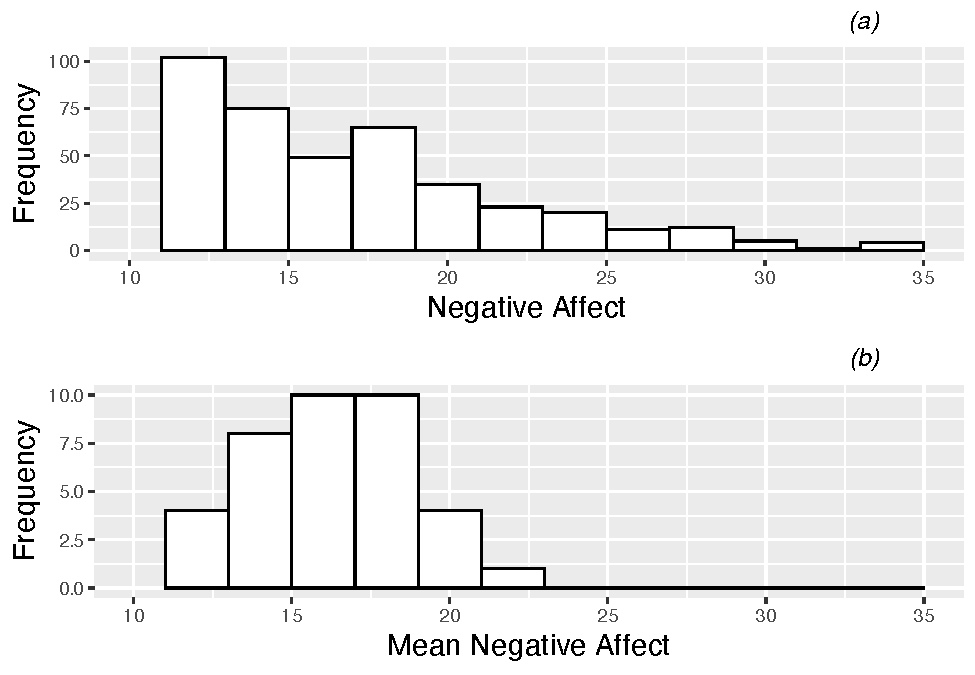
\includegraphics[width=0.6\linewidth]{bookdown-bysh_files/figure-latex/mli-hist1-1} 

}

\caption{Histogram of the continuous Level One response (negative effect). Plot (a) contains all 497 performances across the 37 musicians, while plot (b) contains one observation per musician (the mean negative affect across all performances).}\label{fig:mli-hist1}
\end{figure}

We can also summarize categorical Level One covariates across all (possibly correlated) observations to get a rough relative comparison of trends. 56.1\% of the 497 performances in our data set were solos, while 27.3\% were large ensembles and 16.5\% were small ensembles. The most common audience type was a public performance (41.0\%), followed by instructors (30.0\%), students (20.1\%), and finally juried recitals (8.9\%). In 30.0\% of performances, the musician played by memory, while 55.1\% used the score and 14.9\% of performances were unspecified.

To generate an initial examination of Level Two covariates, we consider a data set with just one observation per subject, since Level Two variables are constant over all performances from the same subject. Then, we can proceed as we did with Level One covariates---using histograms to illustrate the distributions of continuous covariates (see Figure \ref{fig:mli-histmat1}) and tables to summarize categorical covariates. For example, we learn that the majority of subjects have positive emotionality scores between 50 and 60, but that several subjects fall into a lengthy lower tail with scores between 20 and 50. A summary of categorical Level Two covariates reveals that among the 37 subjects (26 female and 11 male), 17 play an orchestral instrument, 15 are vocal performers, and 5 play a keyboard instrument.

\begin{figure}

{\centering 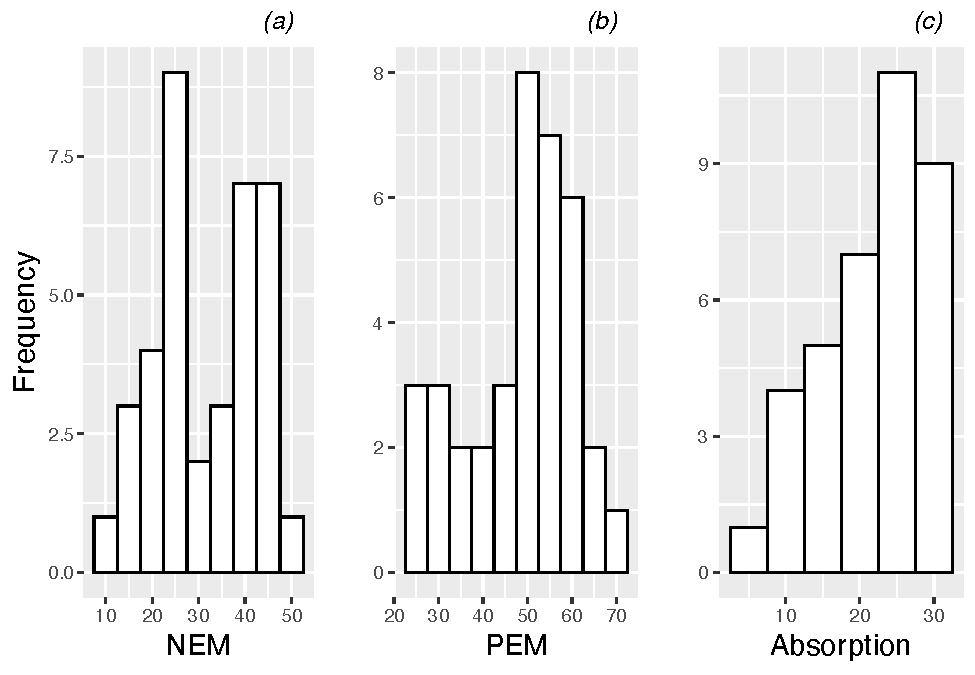
\includegraphics[width=0.6\linewidth]{bookdown-bysh_files/figure-latex/mli-histmat1-1} 

}

\caption{Histograms of the 3 continuous Level Two covariates (negative emotionality (NEM), positive emotionality (PEM), and absorption).  Each plot contains one observation per musician.}\label{fig:mli-histmat1}
\end{figure}

\hypertarget{explore2}{%
\subsection{Exploratory Analyses: Bivariate Summaries}\label{explore2}}

The next step in an initial exploratory analysis is the examination of numerical and graphical summaries of relationships between model covariates and responses. In examining these bivariate relationships, we hope to learn: (1) if there is a general trend suggesting that as the covariate increases the response either increases or decreases, (2) if subjects at certain levels of the covariate tend to have similar mean responses (low variability), and (3) if the variation in the response differs at different levels of the covariate (unequal variability).

As with individual variables, we will begin by treating all 497 performances recorded as independent observations, even though blocks of 15 or so performances were performed by the same musician. For categorical Level One covariates, we can generate boxplots against negative affect as in Figure \ref{fig:mli-boxscatmat1}, plots (a) and (b). From these boxplots, we see that lower levels of performance anxiety seem to be associated with playing in large ensembles and playing in front of an instructor. For our lone continuous Level One covariate (number of previous performances), we can generate a scatterplot against negative affect as in plot (c) from Figure \ref{fig:mli-boxscatmat1}, adding a fitted line to illustrate general trends upward or downward. From this scatterplot, we see that negative affect seems to decrease slightly as a subject has more experience.

To avoid the issue of dependent observations in our three plots from Figure \ref{fig:mli-boxscatmat1}, we could generate separate plots for each subject and examine trends within and across subjects. These ``lattice plots'' \index{lattice plot} are illustrated in Figures \ref{fig:mli-lattice1}, \ref{fig:mli-lattice2}, and \ref{fig:mli-lattice3}; we discuss such plots more thoroughly in Chapter \ref{ch-lon}. While general trends are difficult to discern from these lattice plots, we can see the variety in subjects in sample size distributions and overall level of performance anxiety. In particular, in Figure \ref{fig:mli-lattice3}, we notice that linear fits for many subjects illustrate the same same slight downward trend displayed in the overall scatterplot in Figure \ref{fig:mli-boxscatmat1}, although some subjects experience increasing anxiety and others exhibit non-linear trends. Having an idea of the range of individual trends will be important when we begin to draw overall conclusions from this study.

\begin{figure}

{\centering 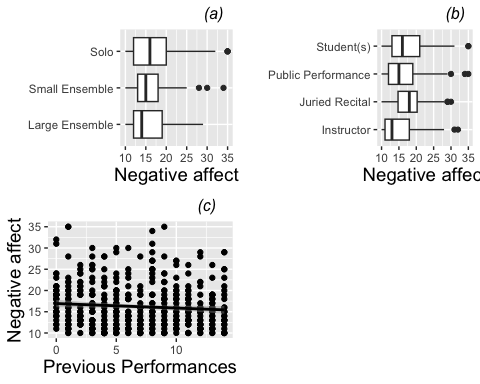
\includegraphics[width=0.6\linewidth]{bookdown-bysh_files/figure-latex/mli-boxscatmat1-1} 

}

\caption{Boxplots of two categorical Level One covariates (performance type (a) and audience type (b)) vs. model response, and scatterplot of one continuous Level One covariate (number of previous diary entries (c)) vs. model response (negative affect).  Each plot contains one observation for each of the 497 performances.}\label{fig:mli-boxscatmat1}
\end{figure}

\begin{figure}

{\centering 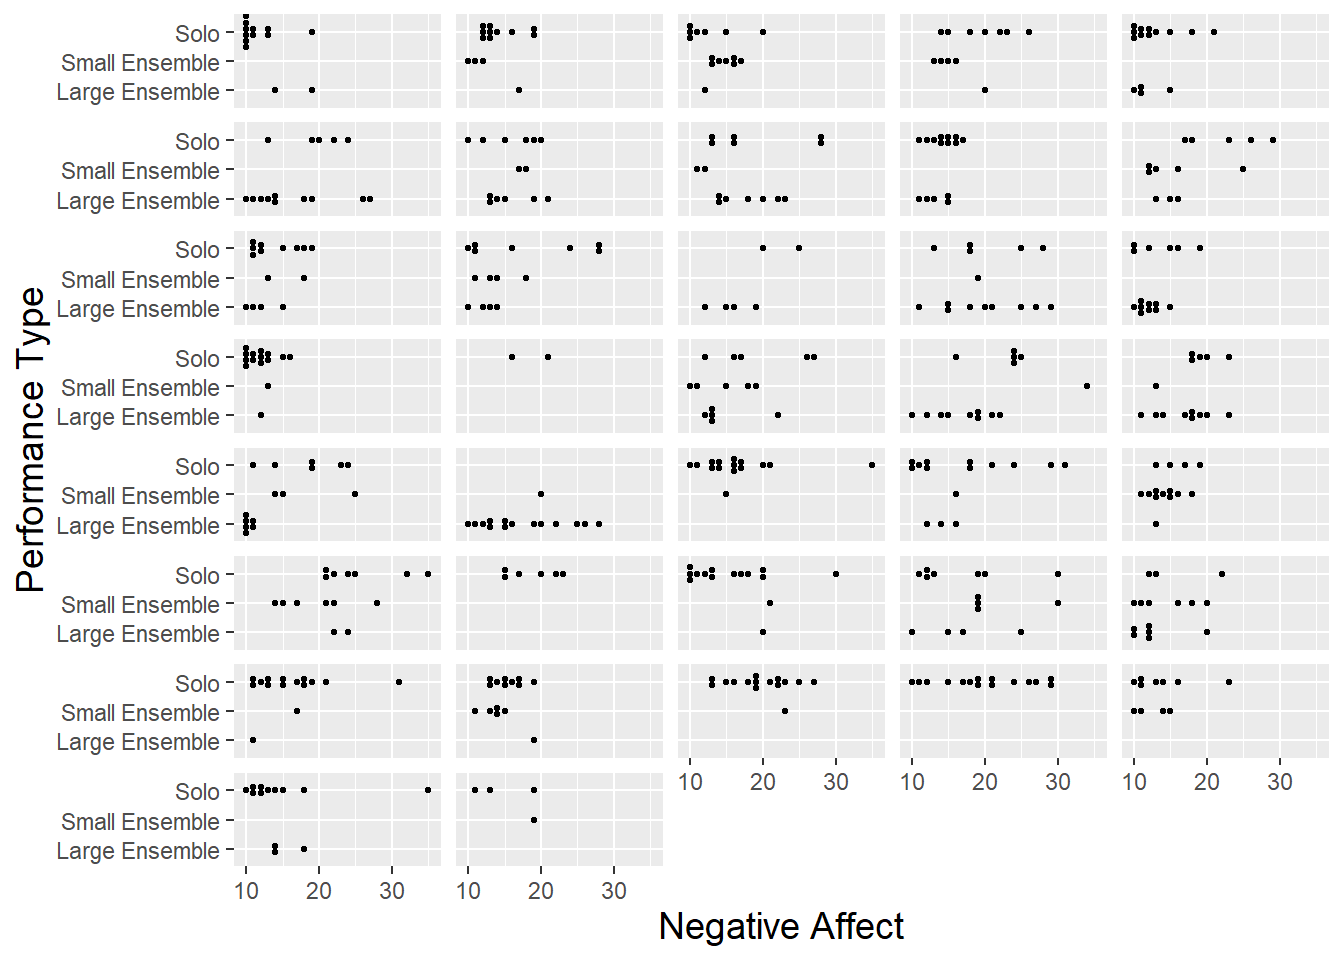
\includegraphics[width=0.6\linewidth]{bookdown-bysh_files/figure-latex/mli-lattice1-1} 

}

\caption{Lattice plot of performance type vs. negative affect, with separate dotplots by subject.}\label{fig:mli-lattice1}
\end{figure}

\begin{figure}

{\centering 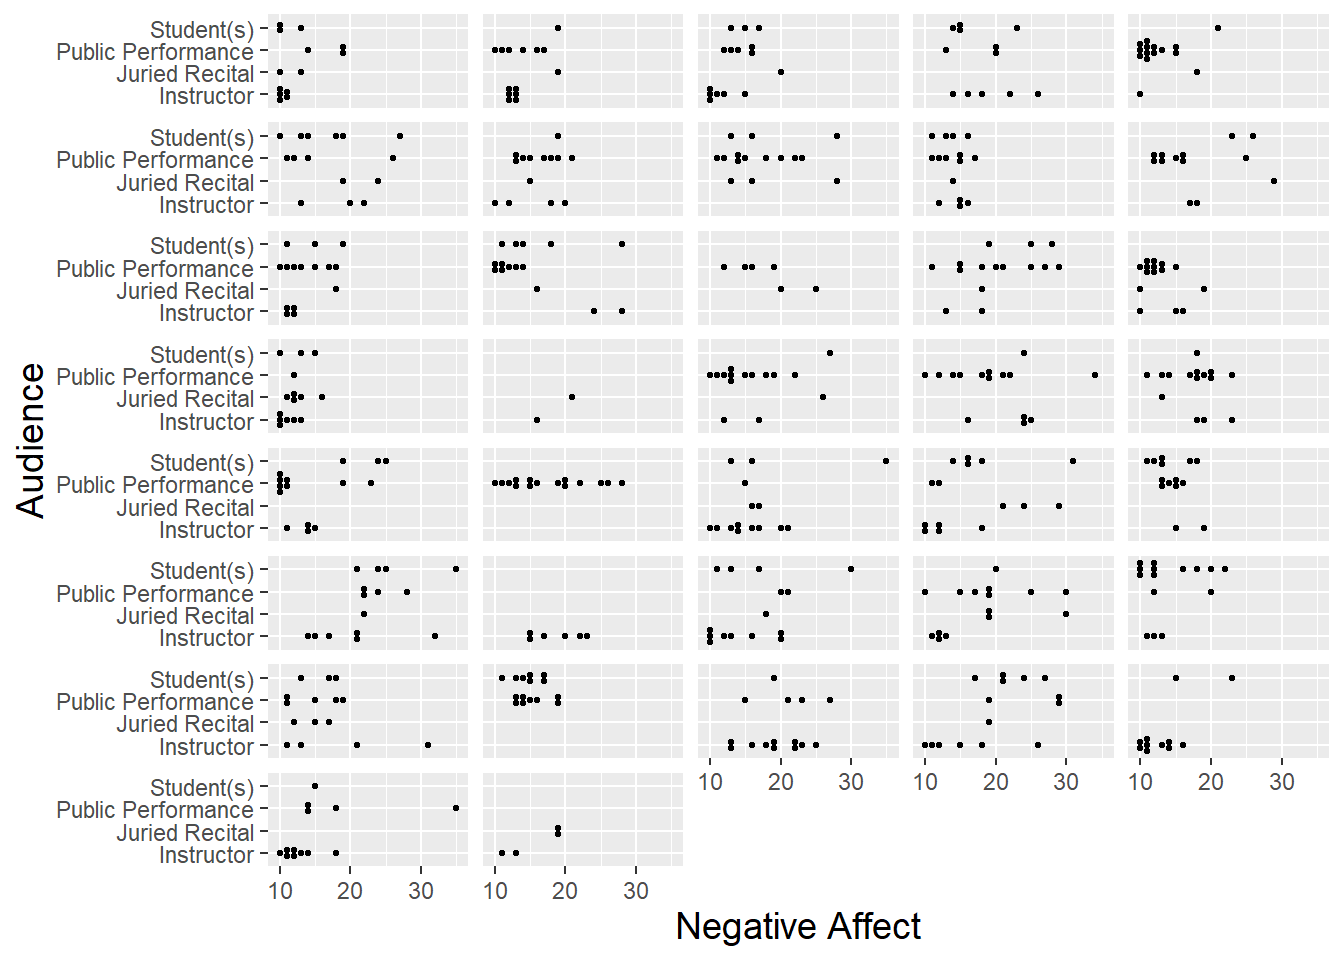
\includegraphics[width=0.6\linewidth]{bookdown-bysh_files/figure-latex/mli-lattice2-1} 

}

\caption{Lattice plot of audience type vs. negative affect, with separate dotplots by subject.}\label{fig:mli-lattice2}
\end{figure}

\begin{figure}

{\centering 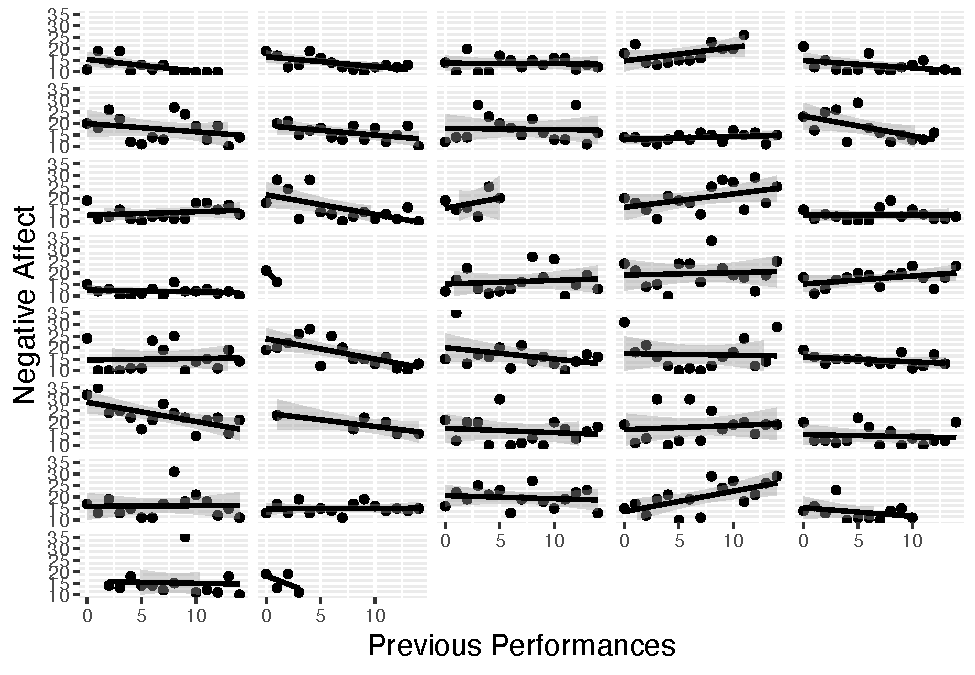
\includegraphics[width=0.6\linewidth]{bookdown-bysh_files/figure-latex/mli-lattice3-1} 

}

\caption{Lattice plot of previous performances vs. negative affect, with separate scatterplots with fitted lines by subject.}\label{fig:mli-lattice3}
\end{figure}

In Figure \ref{fig:mli-boxmat1}, we use boxplots to examine the relationship between our primary categorical Level Two covariate (instrument) and our continuous model response. Plot (a) uses all 497 performances, while plot (b) uses one observation per subject (the mean performance anxiety across all performances) regardless of how many performances that subject had. Naturally, plot (b) has a more condensed range of values, but both plots seem to support the notion that performance anxiety is slightly lower for vocalists and maybe a bit higher for keyboardists

\begin{figure}

{\centering 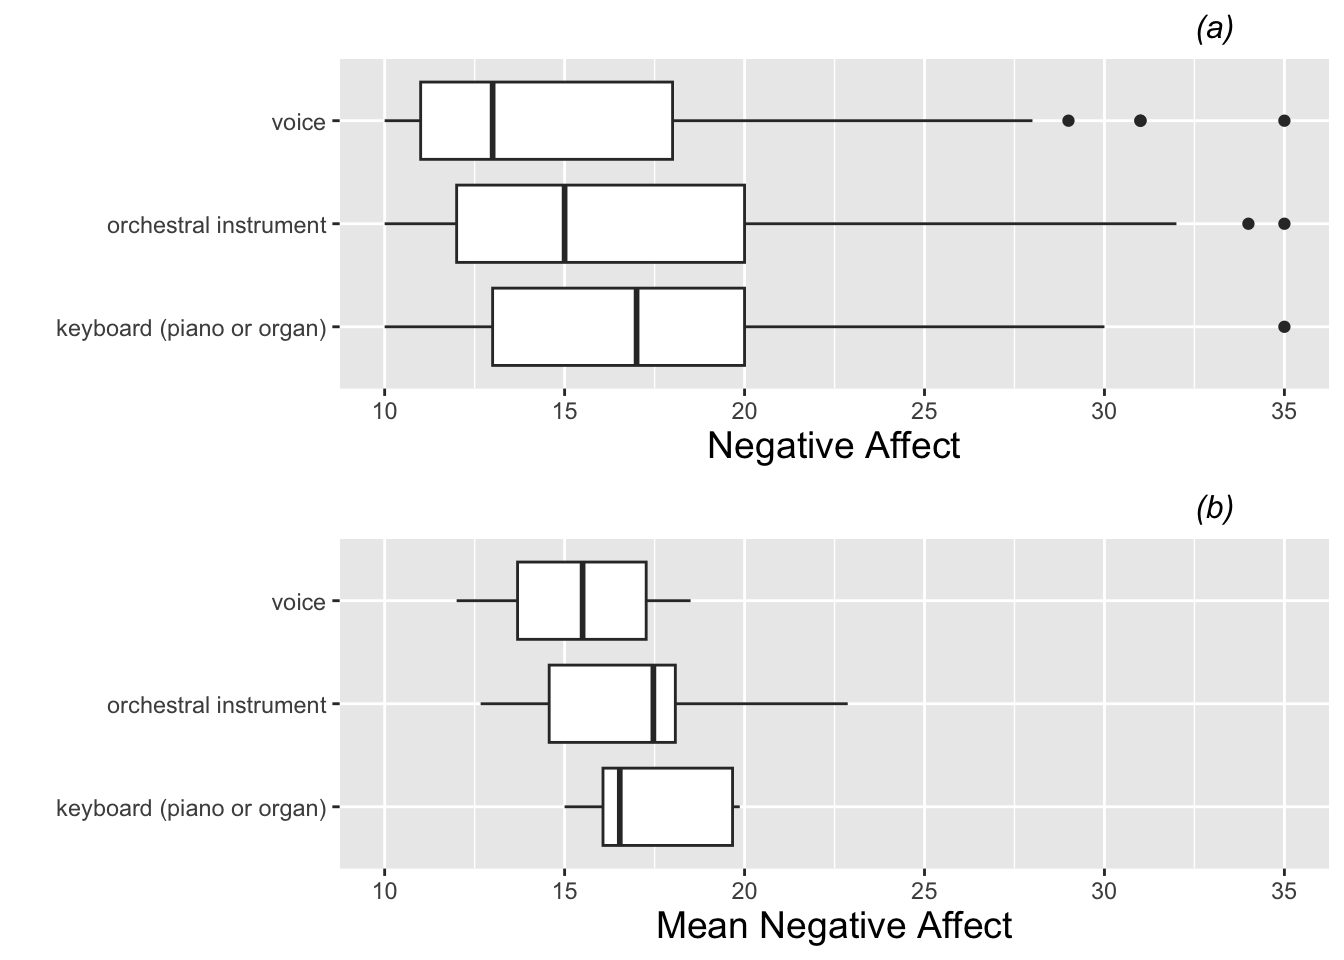
\includegraphics[width=0.6\linewidth]{bookdown-bysh_files/figure-latex/mli-boxmat1-1} 

}

\caption{Boxplots of the categorical Level Two covariate (instrument) vs. model response (negative affect).  Plot (a) is based on all 497 observations from all 37 subjects, while plot (b) uses only one observation per subject.}\label{fig:mli-boxmat1}
\end{figure}

In Figure \ref{fig:mli-scatmat1}, we use scatterplots to examine the relationships between continuous Level Two covariates and our model response. Performance anxiety appears to vary little with a subject's positive emotionality, but there is some evidence to suggest that performance anxiety increases with increasing negative emotionality and absorption level. Plots based on mean negative affect, with one observation per subject, support conclusions based on plots with all observations from all subjects; indeed the overall relationships are in the same direction and of the same magnitude.

\begin{figure}

{\centering 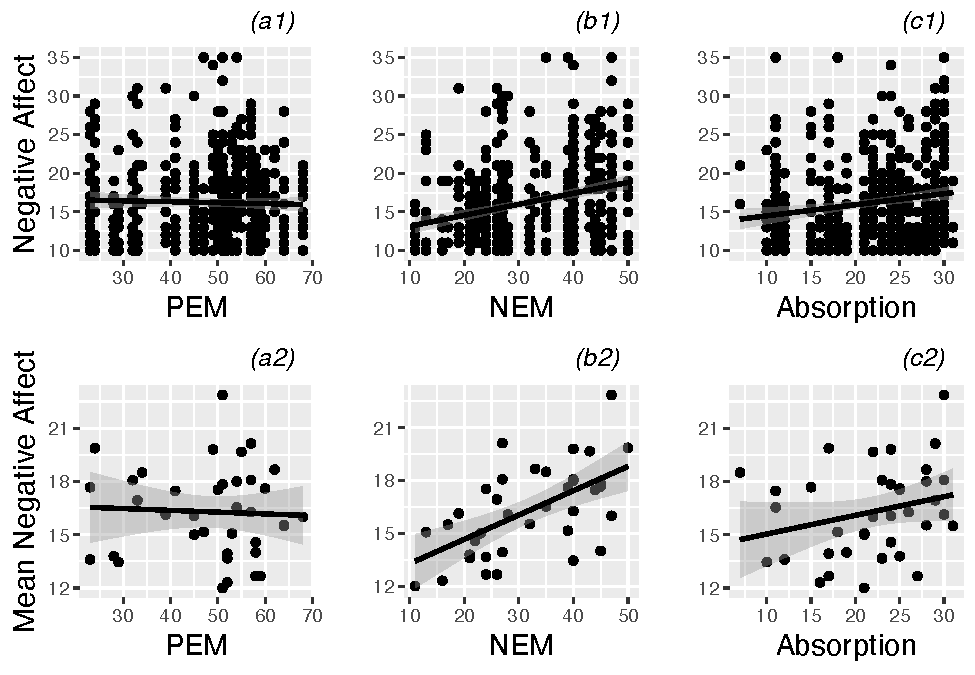
\includegraphics[width=0.6\linewidth]{bookdown-bysh_files/figure-latex/mli-scatmat1-1} 

}

\caption{ Scatterplots of continuous Level Two covariates (positive emotionality (PEM), negative emotionality (NEM), and absorption) vs. model response (negative affect).  The top plots (a1, b1, c1) are based on all 497 observations from all 37 subjects, while the bottom plots (a2, b2, c2) use only one observation per subject.}\label{fig:mli-scatmat1}
\end{figure}

Of course, any graphical analysis is exploratory, and any notable trends at this stage should be checked through formal modeling. At this point, a statistician begins to ask familiar questions such as:

\begin{itemize}
\tightlist
\item
  which characteristics of individual performances are most associated with performance anxiety?
\item
  which characteristics of study participants are most associated with performance anxiety?
\item
  are any of these associations statistically significant?
\item
  does the significance remain after controlling for other covariates?
\item
  how do we account for the lack of independence in performances by the same musician?
\end{itemize}

As you might expect, answers to these questions will arise from proper consideration of variability and properly identified statistical models.

\hypertarget{twolevelmodeling}{%
\section{Two level modeling: preliminary considerations}\label{twolevelmodeling}}

\hypertarget{multregr}{%
\subsection{Ignoring the two level structure (not recommended)}\label{multregr}}

Armed with any statistical software package, it would be relatively simple to take our complete data set of 497 observations and run a multiple linear least squares regression model seeking to explain variability in negative affect with a number of performance-level or musician-level covariates. As an example, output from a model with two binary covariates (Does the subject play an orchestral instrument? and, Was the performance a large ensemble?) is presented below. Do you see any problems with this approach?

\begin{Shaded}
\begin{Highlighting}[]
\CommentTok{# Linear least square regression model with LINE conditions}
\NormalTok{modelc0 <-}\StringTok{ }\KeywordTok{lm}\NormalTok{(na }\OperatorTok{~}\StringTok{ }\NormalTok{orch }\OperatorTok{+}\StringTok{ }\NormalTok{large }\OperatorTok{+}\StringTok{ }\NormalTok{orch}\OperatorTok{:}\NormalTok{large, }\DataTypeTok{data =}\NormalTok{ music)}
\end{Highlighting}
\end{Shaded}

\begin{verbatim}
##             Estimate Std. Error t value   Pr(>|t|)
## (Intercept)  15.7212     0.3591 43.7785 5.548e-172
## orch          1.7887     0.5516  3.2426  1.265e-03
## large        -0.2767     0.7910 -0.3498  7.266e-01
## orch:large   -1.7087     1.0621 -1.6088  1.083e-01
\end{verbatim}

\begin{verbatim}
##  R squared =  0.02782 
##  Residual standard error =  5.179
\end{verbatim}

Other than somewhat skewed residuals, residual plots (not shown) do not indicate any major problems with the LLSR model. However, another key assumption in these models is the independence of all observations. While we might reasonably conclude that responses from different study participants are independent (although possibly not if they are members of the same ensemble group), it is not likely that the 15 or so observations taken over multiple performances from a single subject are similarly independent. If a subject begins with a relatively high level of anxiety (compared to other subjects) before their first performance, chances are good that they will have relatively high anxiety levels before subsequent performances. Thus, multiple linear least squares regression using all 497 observations is not advisable for this study (or multilevel data sets in general).

\hypertarget{twostage}{%
\subsection{A two-stage modeling approach (better but imperfect)}\label{twostage}}

If we assume that the 37 study participants can reasonably be considered to be independent, we could use traditional linear least squares regression techniques to analyze data from this study if we could condense each subject's set of responses to a single meaningful outcome. Candidates for this meaningful outcome include a subject's last performance anxiety measurement, average performance anxiety, minimum anxiety level, etc. For example, in clinical trials, data is often collected over many weekly or monthly visits for each patient, except that many patients will drop out early for many reasons (e.g., lack of efficacy, side effects, personal reasons). In these cases, treatments are frequently compared using ``last-value-carried-forward'' methods---the final visit of each patient is used as the primary outcome measure, regardless of how long they remained in the study. However, ``last-value-carried-forward'' and other summary measures feel inadequate, since we end up ignoring much of the information contained in the multiple measures for each individual. A more powerful solution is to model performance anxiety at multiple levels.

We will begin by considering all performances by a single individual. For instance, consider the 15 performances for which Musician \#22 recorded a diary, illustrated in Table \ref{tab:table2chp8}.

\begin{table}

\caption{\label{tab:table2chp8}Data from the 15 performances of Musician 22}
\centering
\resizebox{\linewidth}{!}{
\begin{tabular}[t]{lrrllrl}
\toprule
  & id & diary & perform\_type & audience & na & instrument\\
\midrule
240 & 22 & 1 & Solo & Instructor & 24 & orchestral instrument\\
241 & 22 & 2 & Large Ensemble & Public Performance & 21 & orchestral instrument\\
242 & 22 & 3 & Large Ensemble & Public Performance & 14 & orchestral instrument\\
243 & 22 & 4 & Large Ensemble & Public Performance & 15 & orchestral instrument\\
244 & 22 & 5 & Large Ensemble & Public Performance & 10 & orchestral instrument\\
\addlinespace
245 & 22 & 6 & Solo & Instructor & 24 & orchestral instrument\\
246 & 22 & 7 & Solo & Student(s) & 24 & orchestral instrument\\
247 & 22 & 8 & Solo & Instructor & 16 & orchestral instrument\\
248 & 22 & 9 & Small Ensemble & Public Performance & 34 & orchestral instrument\\
249 & 22 & 10 & Large Ensemble & Public Performance & 22 & orchestral instrument\\
\addlinespace
250 & 22 & 11 & Large Ensemble & Public Performance & 19 & orchestral instrument\\
251 & 22 & 12 & Large Ensemble & Public Performance & 18 & orchestral instrument\\
252 & 22 & 13 & Large Ensemble & Public Performance & 12 & orchestral instrument\\
253 & 22 & 14 & Large Ensemble & Public Performance & 19 & orchestral instrument\\
254 & 22 & 15 & Solo & Instructor & 25 & orchestral instrument\\
\bottomrule
\end{tabular}}
\end{table}

Does this musician tend to have higher anxiety levels when he is playing in a large ensemble or playing in front of fellow students? Which factor is the biggest determinant of anxiety for a performance by Musician \#22? We can address these questions through multiple LLSR applied to only Musician \#22's data, using appropriate indicator variables for factors of interest.

Let \(Y_{22j}\) be the performance anxiety score of Musician \#22 before performance \(j\). Consider the observed performances for Musician \#22 to be a random sample of all conceivable performances by that subject. If we are initially interested in examining the effect of playing in a large ensemble, we can model the performance anxiety for Musician \#22 according to the model:

\begin{equation}
Y_{22j}=a_{22}+b_{22}\textrm{LargeEns}_{22j}+\epsilon_{22j} \textrm{ where } \epsilon_{22j}\sim N(0,\sigma^2) \textrm{ and }
\label{eq:level1a}
\end{equation}
\[ \textrm{LargeEns}_{j} =
\left\lbrace
\begin{tabular}{l l} 
1 & if `perf\_type` = Large Ensemble \\
0 & if `perf\_type` = Solo or Small Ensemble. 
\end{tabular}\right.
\]
The parameters in this model (\(a_{22}\), \(b_{22}\), and \(\sigma^2\)) can be estimated through least squares methods. \(a_{22}\) represents the true intercept for Musician \#22---the expected anxiety score for Musician \#22 when performance type is a Solo or Small Ensemble (\(\textrm{LargeEns}=0\)), or the true average anxiety for Musician \#22 over all Solo or Small Ensemble performances he may conceivably give. \(b_{22}\) represents the true slope for Musician \#22---the expected increase in performance anxiety for Musician \#22 when performing as part of a Large Ensemble rather than in a Small Ensemble or as a Solo, or the true average difference in anxiety scores for Musician \#22 between Large Ensemble performances and other types. Finally, the \(\epsilon_{22j}\) terms represent the deviations of Musician \#22's actual performance anxiety scores from the expected scores under this model---the part of Musician \#22's anxiety before performance \(j\) that is not explained by performance type. The variability in these deviations from the regression model is denoted by \(\sigma^2\).

For Subject 22, we estimate \(\hat{a}_{22}=24.5\), \(\hat{b}_{22}=-7.8\), and \(\hat{\sigma}=4.8\). Thus, according to our simple linear regression model, Subject 22 had an estimated anxiety score of 24.5 before Solo and Small Ensemble performances, and 16.7 (7.8 points lower) before Large Ensemble performances. With an \(R^2\) of 0.425, the regression model explains a moderate amount (42.5\%) of the performance-to-performance variability in anxiety scores for Subject 22, and the trend toward lower scores for large ensemble performances is statistically significant at the 0.05 level (t(13)=-3.10, p=.009).

\begin{Shaded}
\begin{Highlighting}[]
\NormalTok{regr.id22 =}\StringTok{ }\KeywordTok{lm}\NormalTok{(na }\OperatorTok{~}\StringTok{ }\NormalTok{large, }\DataTypeTok{data =}\NormalTok{ id22)}
\end{Highlighting}
\end{Shaded}

\begin{verbatim}
##             Estimate Std. Error t value  Pr(>|t|)
## (Intercept)   24.500       1.96  12.503 1.275e-08
## large         -7.833       2.53  -3.097 8.504e-03
\end{verbatim}

\begin{verbatim}
##  R squared =  0.4245 
##  Residual standard error =  4.8
\end{verbatim}

We could continue trying to build a better model for Subject 22, adding indicators for audience and memory, and even adding a continuous variable representing the number of previous performance where a diary was kept. As our model R-square value increased, we would be explaining a larger proportion of Subject 22's performance-to-performance variability in anxiety. It would not, however, improve our model to incorporate predictors for age, gender, or even negative emotionality based on the MPQ---why is that?

For the present time, we will model Subject 22's anxiety scores for his 15 performances using the model given by Equation \eqref{eq:level1a}, with a lone indicator variable for performing in a Large Ensemble. We can then proceed to fit the LLSR model in Equation \eqref{eq:level1a} to examine the effect of performing in a Large Ensemble for each of the 37 subjects in this study. These are called \textbf{Level One models} \index{level one model}. As displayed in Figure \ref{fig:mli-histmat2}, there is considerable variability in the fitted intercepts and slopes among the 37 subjects. Mean performance anxiety scores for Solos and Small Ensembles range from 11.6 to 24.5, with a median score of 16.7, while mean differences in performance anxiety scores for Large Ensembles compared to Solos and Small Ensembles range from -7.9 to 5.0, with a median difference of -1.7. Can these differences among individual musicians be explained by (performance-invariant) characteristics associated with each individual, such as gender, age, instrument, years studied, or baseline levels of personality measures? Questions like these can be addressed through further statistical modeling.

\begin{figure}

{\centering 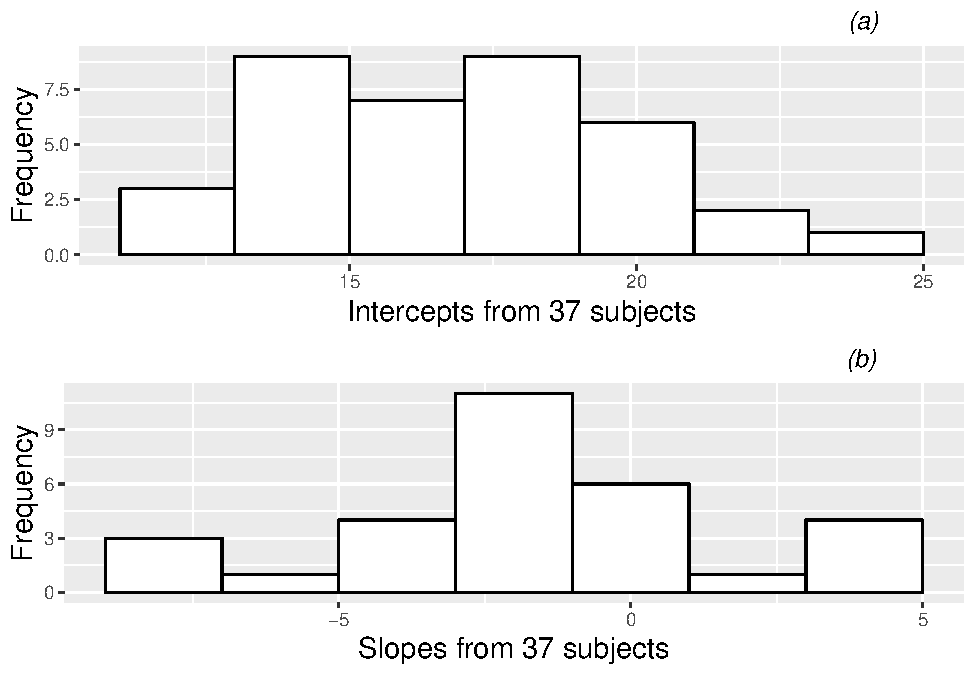
\includegraphics[width=0.6\linewidth]{bookdown-bysh_files/figure-latex/mli-histmat2-1} 

}

\caption{Histograms of intercepts and slopes from fitting simple regression models by subject, where each model contained a single binary predictor indicating if a performance was part of a large ensemble.}\label{fig:mli-histmat2}
\end{figure}

As an illustration, we can consider whether or not there are significant relationships between individual regression parameters (intercepts and slopes) and instrument played. From a modeling perspective, we would build a system of two \textbf{Level Two models} \index{level two model} to predict the fitted intercept (\(a_{i}\)) and fitted slopes (\(b_{i}\)) for Subject \(i\):

\begin{align}
a_{i} & =  \alpha_{0}+\alpha_{1}\textrm{Orch}_{i}+u_{i}
\label{eq:level2s0}  \\
b_{i} & =  \beta_{0}+\beta_{1}\textrm{Orch}_{i}+v_{i}
\label{eq:level2s1}
\end{align}
where \(\textrm{Orch}_{i}=1\) if Subject \(i\) plays an orchestral instrument and \(\textrm{Orch}_{i}=0\) if Subject \(i\) plays keyboard or is a vocalist. Note that, at Level Two, our response variables are not observed measurements such as performance anxiety scores, but rather the fitted regression coefficients from the Level One models fit to each subject. (Well, in our theoretical model, the responses are actually the true intercepts and slopes from Level One models for each subject, but in reality, we have to use our estimated slopes and intercepts.)

Exploratory data analysis (see boxplots by instrument in Figure \ref{fig:mli-boxmat2}) suggests that subjects playing orchestral instruments have higher intercepts than vocalists or keyboardists, and that orchestral instruments are associated with slight lower (more negative) slopes, although with less variability that the slopes of vocalists and keyboardists. These trends are borne out in regression modeling. If we fit Equations \eqref{eq:level2s0} and \eqref{eq:level2s1} using fitted intercepts and slopes as our response variables, we obtain the following estimated parameters: \(\hat{\alpha}_{0}=16.3\), \(\hat{\alpha}_{1}=1.4\), \(\hat{\beta}_{0}=-0.8\), and \(\hat{\beta}_{1}=-1.4\). Thus, the intercept (\(a_{i}\)) and slope (\(b_{i}\)) for Subject \(i\) can be modeled as:

\begin{align}
\hat{a}_{i} & = 16.3+1.4\textrm{Orch}_{i}+u_{i}
\label{eq:level2s0hat}  \\
\hat{b}_{i} & = -0.8-1.4\textrm{Orch}_{i}+v_{i}
\nonumber
\end{align}
where \(a_{i}\) is the true mean negative affect when Subject \(i\) is playing solos or small ensembles, and \(b_{i}\) is the true mean difference in negative affect for Subject \(i\) between large ensembles and other performance types. Based on these models, average performance anxiety before solos and small ensembles is 16.3 for vocalists and keyboardists, but 17.7 (1.4 points higher) for orchestral instrumentalists. Before playing in large ensembles, vocalists and instrumentalists have performance anxiety (15.5) which is 0.8 points lower, on average, than before solos and small ensembles, while subjects playing orchestral instruments experience an average difference of 2.2 points, producing an average performance anxiety of 15.5 before playing in large ensembles just like subjects playing other instruments. However, the difference between orchestral instruments and others does not appear to be statistically significant for either intercepts (t=1.424, p=0.163) or slopes (t=-1.168, p=0.253).

\begin{figure}

{\centering 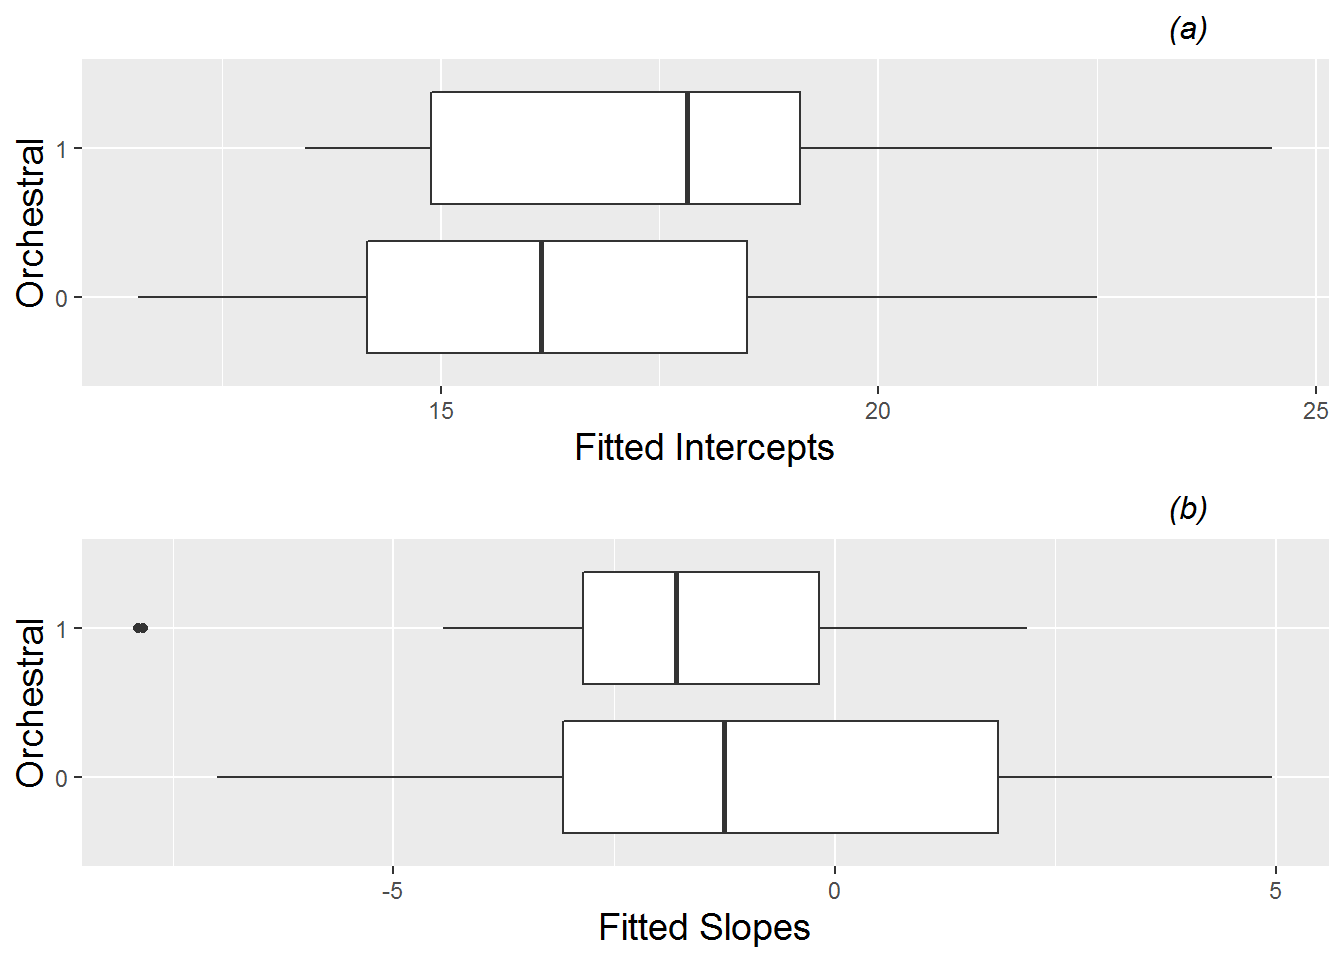
\includegraphics[width=0.6\linewidth]{bookdown-bysh_files/figure-latex/mli-boxmat2-1} 

}

\caption{Boxplots of fitted intercepts (plot (a)) and slopes (plot (b)) by orchestral instrument (1) vs. keyboard or vocalist (0).}\label{fig:mli-boxmat2}
\end{figure}

This two stage modeling process does have some drawbacks. Among other things, (1) it weights every subject the same regardless of the number of diary entries we have, (2) it responds to missing individual slopes (from 7 subjects who never performed in a large ensemble) by simply dropping those subjects, and (3) it does not share strength effectively across individuals. These issues can be better handled through a unified multilevel modeling framework which we will develop over the remainder of this section.

\hypertarget{twolevelmodelingunified}{%
\section{Two level modeling: a unified approach}\label{twolevelmodelingunified}}

\hypertarget{ourframework}{%
\subsection{Our framework}\label{ourframework}}

For the unified approach, we will still envision two levels of models as in section \ref{twostage}, but we will use likelihood-based methods for parameter estimation rather than ordinary least squares to address the drawbacks associated with the two-stage approach. To illustrate the unified approach, we will first generalize the models presented in section \ref{twostage}. Let \(Y_{ij}\) be the performance anxiety score of the \(i^{th}\) subject before performance \(j\). If we are initially interested in examining the effects of playing in a large ensemble and playing an orchestral instrument, then we can model the performance anxiety for Subject \(i\) in performance \(j\) with the following system of equations:

\begin{itemize}
\tightlist
\item
  Level One:
  \begin{equation*}
  Y_{ij} = a_{i}+b_{i}\textrm{LargeEns}_{ij}+\epsilon_{ij}
  \end{equation*}
\item
  Level Two:
  \begin{align*}
  a_{i} & = \alpha_{0}+\alpha_{1}\textrm{Orch}_{i}+u_{i} \\
  b_{i} & = \beta_{0}+\beta_{1}\textrm{Orch}_{i}+v_{i},
  \end{align*}
\end{itemize}

In this system, there are 4 key \textbf{fixed effects} to estimate: \(\alpha_{0}\), \(\alpha_{1}\), \(\beta_{0}\) and \(\beta_{1}\). Fixed effects are the fixed but unknown population effects associated with certain covariates. The intercepts and slopes for each subject from Level One, \(a_{i}\) and \(b_{i}\), don't need to be formally estimated as we did in section \ref{twostage}; they serve to conceptually connect Level One with Level Two. In fact, by substituting the two Level Two equations into the Level One equation, we can view this two-level system of models as a single \textbf{Composite Model} \index{composite model} without \(a_{i}\) and \(b_{i}\):

\begin{align*}
Y_{ij} & = [\alpha_{0}+\alpha_{1}\textrm{Orch}_{i}+\beta_{0}\textrm{LargeEns}_{ij}+\beta_{1}\textrm{Orch}_{i}\textrm{LargeEns}_{ij}] \\
 & \textrm{} + [u_{i}+v_{i}\textrm{LargeEns}_{ij}+\epsilon_{ij}]
\end{align*}

From this point forward, when building multilevel models, we will use Greek letters (such as \(\alpha_{0}\)) to denote final fixed effects model parameters to be estimated empirically, and Roman letters (such as \(a_{0}\)) to denote preliminary fixed effects parameters at lower levels. Variance components that will be estimated empirically will be denoted with \(\sigma\) or \(\rho\), while terms such as \(\epsilon\) and \(u_{i}\) represent error terms. In our framework, we can estimate final parameters directly without first estimating preliminary parameters, which can be seen with the Composite Model formulation (although we can obtain estimates of preliminary parameters in those occasional cases when they are of interest to us). Note that when we model a slope term like \(b_{i}\) from Level One using Level Two covariates like \(\textrm{Orch}_{i}\), the resulting Composite Model contains a \textbf{cross-level interaction term}, \index{cross-level interaction} denoting that the effect of \(\textrm{LargeEns}_{ij}\) depends on the instrument played.

Furthermore, with a binary predictor at Level Two such as instrument, we can write out what our Level Two model looks like for those who play keyboard or are vocalists (\(\textrm{Orch}_{i}=0\)) and those who play orchestral instruments (\(\textrm{Orch}_{i}=1\)):

\begin{itemize}
\tightlist
\item
  Keyboardists and Vocalists (\(\textrm{Orch}_{i}=0\))
\end{itemize}

\begin{align*}
a_{i} & = \alpha_{0}+u_{i} \\
b_{i} & = \beta_{0}+v_{i}
\end{align*}

\begin{itemize}
\tightlist
\item
  Orchestral instrumentalists (\(\textrm{Orch}_{i}=1\))
\end{itemize}

\begin{align*}
a_{i} & = (\alpha_{0}+\alpha_{1})+u_{i} \\
b_{i} & = (\beta_{0}+\beta_{1})+v_{i}
\label{eq:level2byorch}
\end{align*}

Writing the Level Two model in this manner helps us interpret the model parameters from our two-level model. In this case, even the Level One covariate is binary, so that we can write out expressions for mean performance anxiety based on our model for four different combinations of instrument played and performance type:

\begin{itemize}
\tightlist
\item
  Keyboardists or vocalists playing solos or small ensembles: \(\alpha_{0}\)
\item
  Keyboardists or vocalists playing large ensembles: \(\alpha_{0}+\beta_{0}\)
\item
  Orchestral instrumentalists playing solos or small ensembles: \(\alpha_{0}+\alpha_{1}\)
\item
  Orchestral instrumentalists playing large ensembles: \(\alpha_{0}+\alpha_{1}+\beta_{0}+\beta_{1}\)
\end{itemize}

\hypertarget{random-vs.-fixed-effects}{%
\subsection{Random vs.~fixed effects}\label{random-vs.-fixed-effects}}

Before we can use likelihood-based methods to estimate our model parameters, we still must define the distributions of our error terms. The error terms \(\epsilon_{ij}\), \(u_{i}\), and \(v_{i}\) represent random effects in our model. In multilevel models, it is important to distinguish between fixed and random effects. Typically, \textbf{fixed effects} \index{fixed effects} describe levels of a factor that we are specifically interested in drawing inferences about, and which would not change in replications of the study. For example, in our music performance anxiety case study, the levels of performance type will most likely remain as solos, small ensembles, and large ensembles even in replications of the study, and we wish to draw specific conclusions about differences between these three types of performances. Thus, performance type would be considered a fixed effect. On the other hand, \textbf{random effects} \index{random effects} describe levels of a factor which can be thought of as a sample from a larger population of factor levels; we are not typically interested in drawing conclusions about specific levels of a random effect, although we are interested in accounting for the influence of the random effect in our model. For example, in our case study the different musicians included can be thought of as a random sample from a population of performing musicians. Although our goal is not to make specific conclusions about differences between any two musicians, we do want to account for inherent differences among musicians in our model, and by doing so, we will be able to draw more precise conclusions about our fixed effects of interest. Thus, musician would be considered a random effect.

\hypertarget{MVN}{%
\subsection{Distribution of errors: the multivariate normal distribution}\label{MVN}}

As part of our multilevel model, we must provide probability distributions to describe the behavior of random effects. Typically, we assume that random effects follow a normal distribution with mean 0 and a variance parameter which must be estimated from the data. For example, at Level One, we will assume that the errors associated with each performance of a particular musician can be described as: \(\epsilon_{ij}\sim N(0,\sigma^2)\). At Level Two, we have one error term (\(u_{i}\)) associated with subject-to-subject differences in intercepts, and one error term (\(v_{i}\)) associated with subject-to-subject differences in slopes. That is, \(u_{i}\) represents the deviation of Subject \(i\) from the mean performance anxiety before solos and small ensembles after accounting for their instrument, and \(v_{i}\) represents the deviation of Subject \(i\) from the mean difference in performance anxiety between large ensembles and other performance types after accounting for their instrument.

In modeling the random behavior of \(u_{i}\) and \(v_{i}\), we must also account for the possibility that random effects at the same level might be correlated. Subjects with higher baseline performance anxiety have a greater capacity for showing decreased anxiety in large ensembles as compared to solos and small ensembles, so we might expect that subjects with larger intercepts (performance anxiety before solos and small ensembles) would have smaller slopes (indicating greater decreases in anxiety before large ensembles). In fact, our fitted Level One intercepts and slopes in this example actually show evidence of a fairly strong negative correlation (\(r=-0.525\), see Figure \ref{fig:mli-scat1}).

\begin{figure}

{\centering 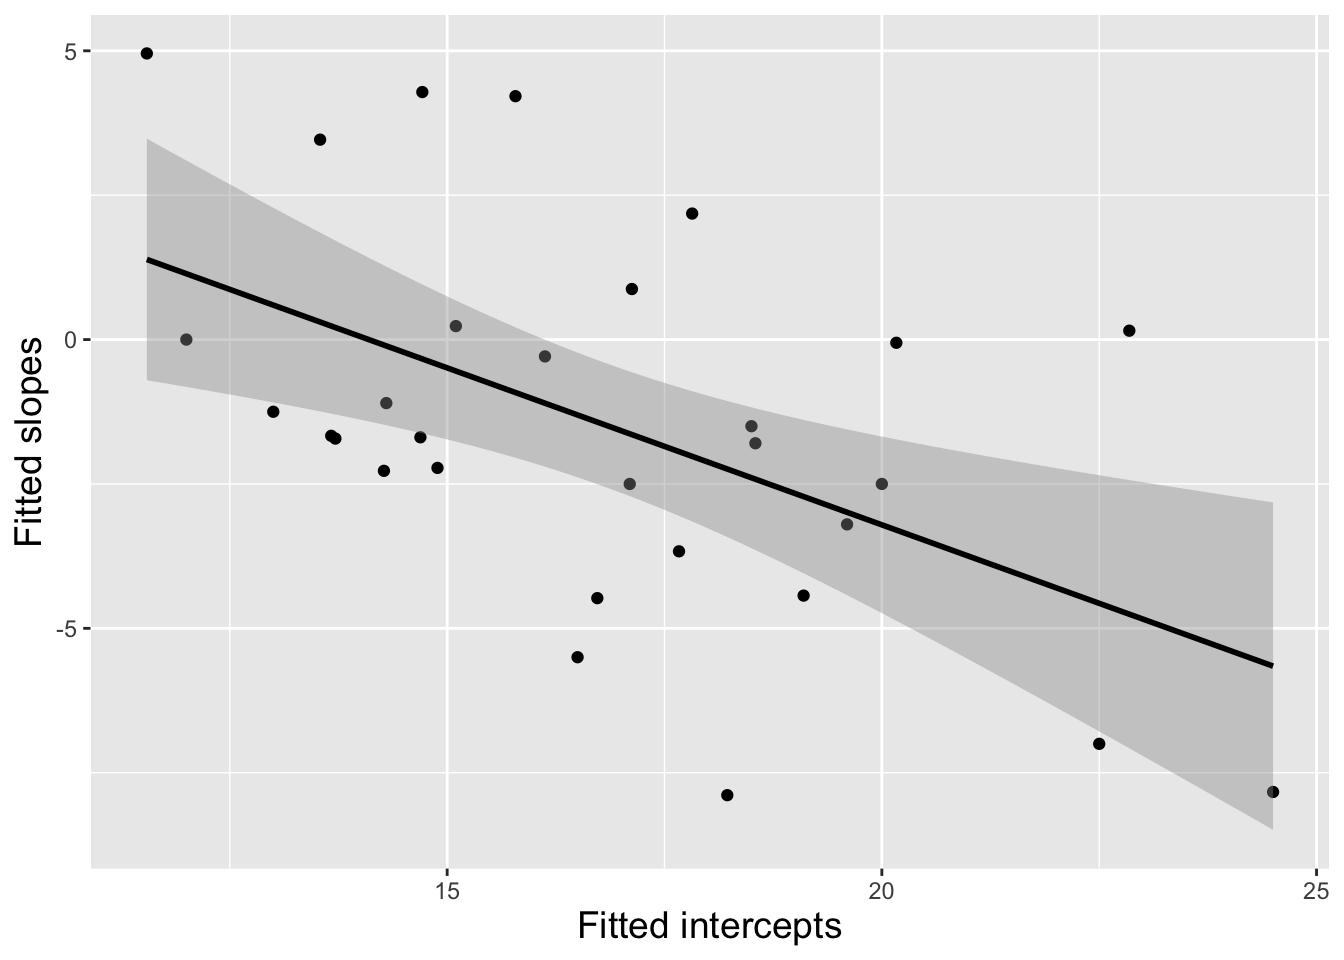
\includegraphics[width=0.6\linewidth]{bookdown-bysh_files/figure-latex/mli-scat1-1} 

}

\caption{Scatterplot with fitted regression line for estimated intercepts and slopes (one point per subject).}\label{fig:mli-scat1}
\end{figure}

To allow for this correlation, the error terms at Level Two can be assumed to follow a \textbf{multivariate normal distribution} \index{multivariate normal distribution} in our unified multilevel model. Mathematically, we can express this as:

\begin{equation*} 
\left[ \begin{array}{c}
            u_{i} \\ v_{i}
          \end{array}  \right] \sim N \left( \left[
          \begin{array}{c}
            0 \\ 0
          \end{array} \right], \left[
          \begin{array}{cc}
            \sigma_{u}^{2} & \rho_{uv}\sigma_{u}\sigma_v \\
            \rho_{uv}\sigma_{u}\sigma_v & \sigma_{v}^{2}
          \end{array} \right] \right) 
\end{equation*}
where \(\sigma_{u}^{2}\) is the variance of the \(u_{i}\) terms, \(\sigma_{v}^{2}\) is the variance of the \(v_{i}\) terms, and \(\sigma_{uv} = \rho_{uv}\sigma_{u}\sigma_v\) is the covariance between the \(u_{i}\) and the \(v_{i}\) terms (i.e., how those two terms vary together).

Note that the correlation \(\rho_{uv}\) between the error terms is simply the covariance \(\sigma_{uv}=\rho_{uv}\sigma_{u}\sigma_{v}\) converted to a \([-1,1]\) scale through the relationship:

\begin{equation*}
\rho_{uv} = \frac{\sigma_{uv}}{\sigma_{u}\sigma_{v}}
\end{equation*}

With this expression, we are allowing each error term to have its own variance (around a mean of 0) and each pair of error terms to have its own covariance (or correlation). Thus, if there are \(n\) equations at Level Two, we can have \(n\) variance terms and \(n(n-1)/2\) covariance terms for a total of \(n + n(n-1)/2\) variance components. These variance components are organized in matrix form, with variance terms along the diagonal and covariance terms in the off-diagonal. In our small example, we have \(n=2\) equations at Level Two, so we have 3 variance components to estimate---2 variance terms (\(\sigma_{u}^{2}\) and \(\sigma_{v}^{2}\)) and 1 correlation (\(\rho_{uv}\)).

The multivariate normal distribution with \(n=2\) is illustrated in Figure \ref{fig:contour-boundary} for two cases: (a) the error terms are uncorrelated (\(\sigma_{uv}=\rho_{uv}=0\)), and (b) the error terms are positively correlated (\(\sigma_{uv}>0\) and \(\rho_{uv} > 0\)). In general, if the errors in intercepts (\(u_{i}\)) are placed on the x-axis and the errors in slopes (\(v_{i}\)) are placed on the y-axis, then \(\sigma_{u}^{2}\) measures spread in the x-direction and \(\sigma_{v}^{2}\) measures spread in the y-direction, while \(\sigma_{uv}\) measures tilt. Positive tilt (\(\sigma_{uv}>0\)) indicates a tendency for errors from the same subject to both be positive or both be negative, while negative tilt (\(\sigma_{uv}<0\)) indicates a tendency for one error from a subject to be positive and the other to be negative. In Figure \ref{fig:contour-boundary}, \(\sigma_{u}^{2}=4\) and \(\sigma_{v}^{2}=1\), so both contour plots show a greater range of errors in the x-direction than the y-direction. Ellipses near the center of the contour plot indicate pairs of \(u_{i}\) and \(v_{i}\) that are more likely. In Figure \ref{fig:contour-boundary} (a) \(\sigma_{uv}=\rho_{uv}=0\), so the axes of the contour plot correspond to the x- and y-axes, but in Figure \ref{fig:contour-boundary} (b) \(\sigma_{uv}=1.5\), so the contour plot tilts up, reflecting a tendency for high values of \(u_{i}\) to be associated with high values of \(v_{i}\).

\begin{figure}

{\centering 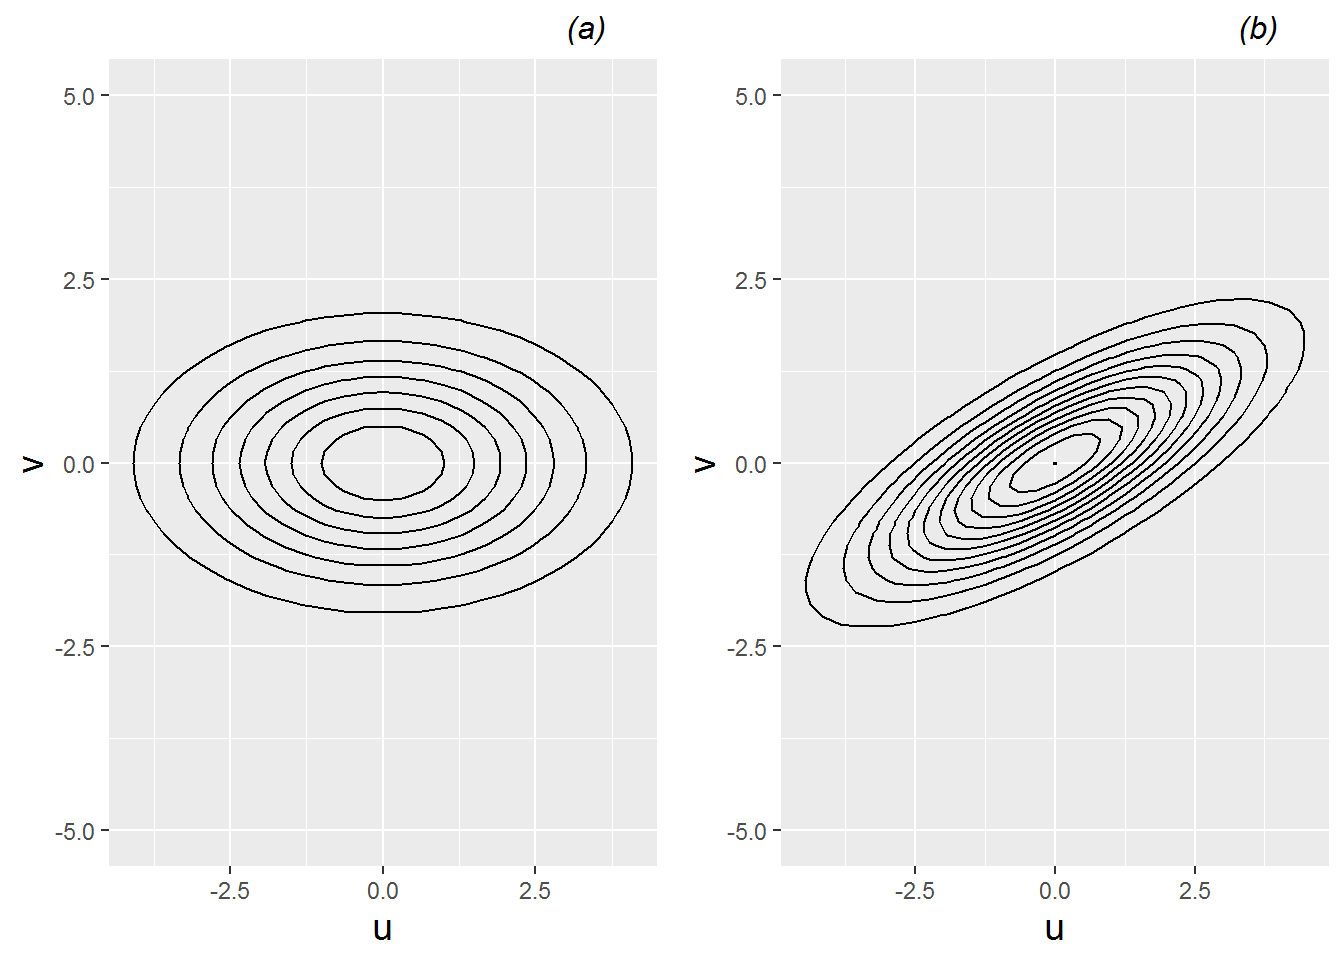
\includegraphics[width=0.6\linewidth]{bookdown-bysh_files/figure-latex/contour-boundary-1} 

}

\caption{Contour plots illustrating a multivariate normal density with (a) no correlation between error terms, and (b) positive correlation between error terms.}\label{fig:contour-boundary}
\end{figure}

\hypertarget{multileveltechnical}{%
\subsection{Technical issues when estimating and testing parameters (Optional)}\label{multileveltechnical}}

Now, our relatively simple two-level model has 8 parameters that need to be estimated: 4 fixed effects (\(\alpha_{0}\), \(\alpha_{1}\), \(\beta_{0}\), and \(\beta_{1}\)), and 4 variance components (\(\sigma^{2}\), \(\sigma_{u}^{2}\), \(\sigma_{v}^{2}\), and \(\sigma_{uv}\)). Note that we use the term \textbf{variance components} \index{variance components} to signify model parameters that describe the behavior of random effects. We can use statistical software, such as the lmer() function from the lme4 package in R, to obtain parameter estimates using our 497 observations. The most common methods for estimating model parameters---both fixed effects and variance components---are maximum likelihood (ML) and \textbf{restricted maximum likelihood (REML)} \index{restricted maximum likelihood (REML)}. The method of maximum likelihood (ML) was introduced in Chapter \ref{ch-beyondmost}, where parameter estimates are chosen to maximize the value of the likelihood function based on observed data. Restricted maximum likelihood (REML) is conditional on the fixed effects, so that the part of the data used for estimating variance components is separated from that used for estimating fixed effects. Thus REML, by accounting for the loss in degrees of freedom from estimating the fixed effects, provides an unbiased estimate of variance components, while ML estimators for variance components are biased under assumptions of normality, since they use estimated fixed effects rather than the true values. REML is preferable when the number of parameters is large or the primary interest is obtaining estimates of model parameters, either fixed effects or variance components associated with random effects. ML should be used if nested fixed effects models are being compared using a likelihood ratio test, although REML is fine for nested models of random effects (with the same fixed effects model). In this text, we will typically report REML estimates unless we are specifically comparing nested models with the same random effects. In most case studies and most models we consider, there is very little difference between ML and REML parameter estimates. Additional details are beyond the scope of this book \citep{Singer2003}.

Note that the multilevel output shown beginning in the next section contains no p-values for performing hypothesis tests. This is primarily because the exact distribution of the test statistics under the null hypothesis (no fixed effect) is unknown, primarily because the exact degrees of freedom is not known \citep{Bates2015}. Finding good approximate distributions for test statistics (and thus good approximate p-values) in multilevel models is an area of active research. In most cases, we can simply conclude that t-values (ratios of parameter estimates to estimated standard errors) with absolute value above 2 indicate significant evidence that a particular model parameter is different than 0. Certain software packages will report p-values corresponding to hypothesis tests for parameters of fixed effects; these packages are typically using conservative assumptions, large-sample results, or approximate degrees of freedom for a t-distribution. In section \ref{multreg-boot}, we introduced the bootstrap as a non-parametric, computational approach for producing confidence intervals for model parameters. In addition, in section \ref{longitudinal-paraboot}, we will introduce a method called the parametric bootstrap which is being used more frequently by researchers to better approximate the distribution of the likelihood test statistic and produce more accurate p-values by simulating data under the null hypothesis \citep{Efron2012}.

\hypertarget{initialmodel}{%
\subsection{An initial model with parameter interpretations}\label{initialmodel}}

The output below contains likelihood-based estimates of our 8 parameters from a two-level model applied to the music performance anxiety data:

\begin{verbatim}
    Linear mixed model fit by REML ['lmerMod'] 
 A)  Formula: na ~ orch + large + orch:large + (large | id) 
        Data: music 
 B)  REML criterion at convergence: 2987 
      
 B2)      AIC      BIC   logLik deviance df.resid  
         3007     3041    -1496     2991      489  
      
     Random effects: 
      Groups   Name        Variance Std.Dev. Corr  
 C)   id       (Intercept)  5.655   2.378          
 D)            large        0.452   0.672    -0.63 
 E)   Residual             21.807   4.670          
 F)  Number of obs: 497, groups:  id, 37 
      
     Fixed effects: 
                 Estimate Std. Error t value 
 G)  (Intercept)   15.930      0.641   24.83 
 H)  orch           1.693      0.945    1.79 
 I)  large         -0.911      0.845   -1.08 
 J)  orch:large    -1.424      1.099   -1.30
\end{verbatim}

This output (except for the capital letters along the left column) was specifically generated by the lmer() function in R; multilevel modeling results from other packages will contain similar elements. Because we will use lmer() output to summarize analyses of case studies in this and following sections, we will spend a little time now orienting ourselves to the most important features in this output.

\begin{itemize}
\tightlist
\item
  A: How our multilevel model is written in R, based on the composite model formulation. For more details, see section \ref{notesr8}.
\item
  B: Measures of model performance. Since this model was fit using REML, this line only contains the REML criterion.
\item
  B2: If the model is fit with ML instead of REML, the measures of performance will contain AIC, BIC, deviance, and the log-likelihood.
\item
  C: Estimated variance components (\(\hat{\sigma}_{u}^2\) and \(\hat{\sigma}_{u}\)) associated with the intercept equation in Level Two.
\item
  D: Estimated variance components (\(\hat{\sigma}_{v}^2\) and \(\hat{\sigma}_{v}\)) associated with the large ensemble effect equation in Level Two, along with the estimated correlation (\(\hat{\rho}_{uv}\)) between the two Level Two error terms.
\item
  E: Estimated variance components (\(\hat{\sigma}^2\) and \(\hat{\sigma}\)) associated with the Level One equation.
\item
  F: Total number of performances where data was collected (Level One observations = 497) and total number of subjects (Level Two observations = 37).
\item
  G: Estimated fixed effect (\(\hat{\alpha}_{0}\)) for the intercept term, along with its standard error and t-value (which is the ratio of the estimated coefficient to its standard error). As described in section \ref{multileveltechnical}, no p-value testing the significance of the coefficient is provided because the exact null distribution of the t-value is unknown.
\item
  H: Estimated fixed effect (\(\hat{\alpha}_{1}\)) for the orchestral instrument effect, along with its standard error and t-value .
\item
  I: Estimated fixed effect (\(\hat{\beta}_{0}\)) for the large ensemble effect, along with its standard error and t-value.
\item
  J: Estimated fixed effect (\(\hat{\beta}_{1}\)) for the interaction between orchestral instruments and large ensembles, along with its standard error and t-value.
\end{itemize}

Assuming the 37 musicians in this study are representative of a larger population of musicians, parameter interpretations for our 8 model parameters are given below:

\begin{itemize}
\tightlist
\item
  Fixed effects:

  \begin{itemize}
  \tightlist
  \item
    \(\hat{\alpha}_{0} = 15.9\). The estimated mean performance anxiety for solos and small ensembles (Large=0) for keyboard players and vocalists (Orch=0) is 15.9.
  \item
    \(\hat{\alpha}_{1} = 1.7\). Orchestral instrumentalists have an estimated mean performance anxiety for solos and small ensembles which is 1.7 points higher than keyboard players and vocalists.
  \item
    \(\hat{\beta}_{0} = -0.9\). Keyboard players and vocalists have an estimated mean decrease in performance anxiety of 0.9 points when playing in large ensembles instead of solos or small ensembles.
  \item
    \(\hat{\beta}_{1} = -1.4\). Orchestral instrumentalists have an estimated mean decrease in performance anxiety of 2.3 points when playing in large ensembles instead of solos or small ensembles, 1.4 points greater than the mean decrease among keyboard players and vocalists.
  \end{itemize}
\item
  Variance components

  \begin{itemize}
  \tightlist
  \item
    \(\hat{\sigma}_{u} = 2.4\). The estimated standard deviation of performance anxiety levels for solos and small ensembles is 2.4 points, after controlling for instrument played.
  \item
    \(\hat{\sigma}_{v} = 0.7\). The estimated standard deviation of differences in performance anxiety levels between large ensembles and other performance types is 0.7 points, after controlling for instrument played.
  \item
    \(\hat{\rho}_{uv} = -0.64\). The estimated correlation between performance anxiety scores for solos and small ensembles and increases in performance anxiety for large ensembles is -0.64, after controlling for instrument played. Those subjects with higher performance anxiety scores for solos and small ensembles tend to have greater decreases in performance anxiety for large ensemble performances.
  \item
    \(\hat{\sigma} = 4.7.\) The estimated standard deviation in residuals for the individual regression models is 4.7 points.
  \end{itemize}
\end{itemize}

Table \ref{tab:table3chp8} shows a side-by-side comparison of estimated coefficients from the approaches described to this point. Underlying assumptions, especially regarding the error and correlation structure, differ, and differences in estimated effects are potentially meaningful. Note that some standard errors are greatly \emph{underestimated} under independence, and that no Level One covariates (such as performance type) can be analyzed under a method such as last-visit-carried-forward which uses one observation per subject. Moving forward, we will employ the unified multilevel approach to maximize the information being used to estimate model parameters and to remain faithful to the structure of the data.

\begin{table}

\caption{\label{tab:table3chp8}Comparison of estimated coefficients and standard errors from the approaches mentioned in this section.}
\centering
\begin{tabular}[t]{lllll}
\toprule
Variable & Independence & TwoStage & LVCF & Multilevel\\
\midrule
Intercept & 15.72(0.36) & 16.28(0.67) & 15.20(1.25) & 15.93(0.64)\\
Orch & 1.79(0.55) & 1.41(0.99) & 1.45(1.84) & 1.69(0.95)\\
Large & -0.28(0.79) & -0.77(0.85) & - & -0.91(0.85)\\
Orch*Large & -1.71(1.06) & -1.41(1.20) & - & -1.42(1.10)\\
\bottomrule
\end{tabular}
\end{table}

Two level modeling as done with the music performance anxiety data usually involves fitting a number of models. Subsequent sections will describe a process of starting with the simplest two-level models and building toward a final model which addresses the research questions of interest.

\hypertarget{sec:buildmodel}{%
\section{Building a multilevel model}\label{sec:buildmodel}}

\hypertarget{buildstrategy}{%
\subsection{Model building strategy}\label{buildstrategy}}

Initially, it is advisable to first fit some simple, preliminary models, in part to establish a baseline for evaluating larger models. Then, we can build toward a final model for description and inference by attempting to add important covariates, centering certain variables, and checking model assumptions. In this study, we are particularly interested in Level Two covariates---those subject-specific variables that provide insight into why individuals react differently in anxiety-inducing situations. To get more precise estimates of the effect of Level Two covariates, we also want to control for Level One covariates that describe differences in individual performances.

Our strategy for building multilevel models will begin with extensive exploratory data analysis at each level. Then, after examining models with no predictors to assess variability at each level, we will first focus on creating a Level One model, starting simple and adding terms as necessary. Next, we will move to Level Two models, again starting simple and adding terms as necessary, beginning with the equation for the intercept term. Finally, we will examine the random effects and variance components, beginning with a full set of error terms and then removing covariance terms and variance terms where advisable (for instance, when parameter estimates are failing to converge or producing impossible or unlikely values). This strategy follows closely with that described by \citet{Bryk2002} and used by \citet{Singer2003}. Singer and Willett further find that the modeled error structure rarely matters in practical contexts. Other model building approaches are certainly possible. \citet{Diggle2002}, for example, begins with a saturated fixed effects model, determines variance components based on that, and then simplifies the fixed part of the model after fixing the random part.

\hypertarget{modela8}{%
\subsection{An initial model: unconditional means or random intercepts}\label{modela8}}

The first model fit in almost any multilevel context should be the \textbf{unconditional means model} \index{unconditional means model}, also called a \textbf{random intercepts model} \index{random intercepts model}. In this model, there are no predictors at either level; rather, the purpose of the unconditional means model is to assess the amount of variation at each level---to compare variability within subject to variability between subjects. Expanded models will then attempt to explain sources of between and within subject variability.

The unconditional means (random intercepts) model, which we will denote as Model A, can be specified either using formulations at both levels:

\begin{itemize}
\tightlist
\item
  Level One:
  \begin{equation*}
  Y_{ij} = a_{i}+\epsilon_{ij} \textrm{ where } \epsilon_{ij}\sim N(0,\sigma^2)
  \end{equation*}
\item
  Level Two:
  \begin{equation*}
  a_{i} = \alpha_{0}+u_{i} \textrm{ where } u_{i}\sim N(0,\sigma_{u}^{2})
  \end{equation*}
\end{itemize}

or as a composite model:
\begin{equation*}
Y_{ij}=\alpha_{0}+u_{i}+\epsilon_{ij}
\end{equation*}
In this model, the performance anxiety scores of subject \(i\) are not a function of performance type or any other Level One covariate, so that \(a_{i}\) is the true mean response of all observations for subject \(i\). On the other hand, \(\alpha_{0}\) is the grand mean -- the true mean of all observations across the entire population. Our primary interest in the unconditional means model is the variance components -- \(\sigma^2\) is the within-person variability, while \(\sigma_{u}^{2}\) is the between-person variability. The name \textbf{random intercepts model} then arises from the Level Two equation for \(a_{i}\): each subject's intercept is assumed to be a random value from a normal distribution centered at \(\alpha_{0}\) with variance \(\sigma_{u}^{2}\).

Using the composite model specification, the unconditional means model can be fit to the music performance anxiety data using statistical software:

\begin{Shaded}
\begin{Highlighting}[]
\CommentTok{#Model A (Unconditional means model)}
\NormalTok{model.a <-}\StringTok{ }\KeywordTok{lmer}\NormalTok{(na }\OperatorTok{~}\StringTok{ }\DecValTok{1} \OperatorTok{+}\StringTok{ }\NormalTok{(}\DecValTok{1} \OperatorTok{|}\StringTok{ }\NormalTok{id), }\DataTypeTok{REML =}\NormalTok{ T, }\DataTypeTok{data =}\NormalTok{ music)}
\end{Highlighting}
\end{Shaded}

\begin{verbatim}
##  Groups   Name        Variance Std.Dev.
##  id       (Intercept)  4.95    2.22    
##  Residual             22.46    4.74
\end{verbatim}

\begin{verbatim}
##  Number of Level Two groups =  37
\end{verbatim}

\begin{verbatim}
##             Estimate Std. Error t value
## (Intercept)    16.24     0.4279   37.94
\end{verbatim}

From this output, we obtain estimates of our three model parameters:

\begin{itemize}
\tightlist
\item
  \(\hat{\alpha}_{0}=16.2=\) the estimated mean performance anxiety score across all performances and all subjects.
\item
  \(\hat{\sigma}^2=22.5=\) the estimated variance in within-person deviations.
\item
  \(\hat{\sigma}_{u}^{2}=5.0=\) the estimated variance in between-person deviations.
\end{itemize}

The relative levels of between- and within-person variabilities can be compared through the \textbf{intraclass correlation coefficient} \index{intraclass correlation coefficient}:

\begin{equation*}
\hat{\rho}=\frac{\textrm{Between-person variability}}{\textrm{Total variability}} = \frac{\hat{\sigma}_{u}^{2}}{\hat{\sigma}_{u}^{2}+\hat{\sigma}^2} = \frac{5.0}{5.0+22.5} = .182.
\end{equation*}
Thus, 18.2\% of the total variability in performance anxiety scores are attributable to differences among subjects. In this particular model, we can also say that the average correlation for any pair of responses from the same individual is a moderately low .182. As \(\rho\) approaches 0, responses from an individual are essentially independent and accounting for the multilevel structure of the data becomes less crucial. However, as \(\rho\) approaches 1, repeated observations from the same individual essentially provide no additional information and accounting for the multilevel structure becomes very important. With \(\rho\) near 0, the \textbf{effective sample size} \index{effective sample size} (the number of independent pieces of information we have for modeling) approaches the total number of observations, while with \(\rho\) near 1, the effective sample size approaches the number of subjects in the study.

\hypertarget{modelb}{%
\section{Binary covariates at Level One and Level Two}\label{modelb}}

\hypertarget{randomslopeandint}{%
\subsection{Random slopes and intercepts model}\label{randomslopeandint}}

The next step in model fitting is to build a good model for predicting performance anxiety scores at Level One (within subject). We will add potentially meaningful Level One covariates---those that vary from performance-to-performance for each individual \index{random slopes and intercepts model}. In this case, mirroring our model from section \ref{twolevelmodeling}, we will include a binary covariate for performance type:

\[ \textrm{LargeEns}_{ij} =
\left\lbrace
\begin{tabular}{l l} 
1 & if `perf\_type` = Large Ensemble \\
0 & if `perf\_type` = Solo or Small Ensemble. 
\end{tabular}\right.
\]
and no other Level One covariates (for now). (Note that we may later also want to include an indicator variable for ``Small Ensemble'' to separate the effects of \texttt{Solo} performances and \texttt{Small\ Ensemble} performances.) The resulting model, which we will denote as Model B, can be specified either using formulations at both levels:

\begin{itemize}
\tightlist
\item
  Level One:
  \begin{equation*}
  Y_{ij} = a_{i}+b_{i}\textrm{LargeEns}_{ij}+\epsilon_{ij}
  \end{equation*}
\item
  Level Two:
  \begin{align*}
  a_{i} & = \alpha_{0}+u_{i} \\
  b_{i} & = \beta_{0}+v_{i}
  \end{align*}
  or as a composite model:
\end{itemize}

\begin{equation*}
Y_{ij}=[\alpha_{0}+\beta_{0}\textrm{LargeEns}_{ij}]+[u_{i}+v_{i}\textrm{LargeEns}_{ij}+\epsilon_{ij}]
\end{equation*}
where \(\epsilon_{ij}\sim N(0,\sigma^2)\) and

\[ \left[ \begin{array}{c}
            u_{i} \\ v_{i}
          \end{array}  \right] \sim N \left( \left[
          \begin{array}{c}
            0 \\ 0
          \end{array} \right], \left[
          \begin{array}{cc}
            \sigma_{u}^{2} & \\
            \rho\sigma_{u}\sigma_{v} & \sigma_{v}^{2}
          \end{array} \right] \right). \]
as discussed in section \ref{MVN}.

In this model, performance anxiety scores for subject \(i\) are assumed to differ (on average) for Large Ensemble performances as compared with Solos and Small Ensemble performances; the \(\epsilon_{ij}\) terms capture the deviation between the true performance anxiety levels for subjects (based on performance type) and their observed anxiety levels. \(\alpha_{0}\) is then the true mean performance anxiety level for Solos and Small Ensembles, and \(\beta_{0}\) is the true mean difference in performance anxiety for Large Ensembles compared to other performance types. As before, \(\sigma^2\) quantifies the within-person variability (the scatter of points around individuals' means by performance type), while now the between-person variability is partitioned into variability in Solo and Small Ensemble scores (\(\sigma_{u}^{2}\)) and variability in differences with Large Ensembles (\(\sigma_{v}^{2}\)).

Using the composite model specification, Model B can be fit to the music performance anxiety data, producing the following output:

\begin{Shaded}
\begin{Highlighting}[]
\CommentTok{#Model B (Add large as Level 1 covariate)}
\NormalTok{model.b <-}\StringTok{ }\KeywordTok{lmer}\NormalTok{(na }\OperatorTok{~}\StringTok{ }\NormalTok{large }\OperatorTok{+}\StringTok{  }\NormalTok{(large }\OperatorTok{|}\StringTok{ }\NormalTok{id), }\DataTypeTok{data =}\NormalTok{ music)}
\end{Highlighting}
\end{Shaded}

\begin{verbatim}
##  Groups   Name        Variance Std.Dev. Corr 
##  id       (Intercept)  6.333   2.517         
##           large        0.743   0.862    -0.76
##  Residual             21.771   4.666
\end{verbatim}

\begin{verbatim}
##  Number of Level Two groups =  37
\end{verbatim}

\begin{verbatim}
##             Estimate Std. Error t value
## (Intercept)   16.730     0.4908   34.09
## large         -1.676     0.5425   -3.09
\end{verbatim}

From this output, we obtain estimates of our six model parameters (2 fixed effects and 4 variance components):

\begin{itemize}
\tightlist
\item
  \(\hat{\alpha}_{0}=16.7=\) the mean performance anxiety level before solos and small ensemble performances.
\item
  \(\hat{\beta}_{0}=-1.7=\) the mean decrease in performance anxiety before large ensemble performances.
\item
  \(\hat{\sigma}^2=21.8=\) the variance in within-person deviations.
\item
  \(\hat{\sigma}_{u}^{2}=6.3=\) the variance in between-person deviations in performance anxiety scores before solos and small ensembles.
\item
  \(\hat{\sigma}_{v}^{2}=0.7=\) the variance in between-person deviations in increases (or decreases) in performance anxiety scores before large ensembles.
\item
  \(\hat{\rho}_{uv}=-0.76=\) the correlation in subjects' anxiety before solos and small ensembles and their differences in anxiety between large ensembles and other performance types.
\end{itemize}

We see that, on average, subjects had a performance anxiety level of 16.7 before solos and small ensembles, and their anxiety levels were 1.7 points lower, on average, before large ensembles, producing an average performance anxiety level before large ensembles of 15.0. According to the t-value listed in R, the difference between large ensembles and other performance types is statistically significant (t=-3.09).

This random slopes and intercepts model is illustrated in Figure \ref{fig:mli-spag1}. The thicker black line shows the overall trends given by our estimated fixed effects: an intercept of 16.7 and a slope of -1.7. Then, each subject is represented by a gray line. Not only do the subjects' intercepts differ (with variance 6.3), but their slopes differ as well (with variance 0.7). Additionally, subjects' slopes and intercepts are negatively associated (with correlation -0.76), so that subjects with greater intercepts tend to have steeper negative slopes. We can compare this model with the random intercepts model from section \ref{modela8}, pictured in Figure \ref{fig:mli-spag0}. With no effect of large ensembles, each subject is represented by a gray line with identical slopes (0) but varying intercepts (with variance 5.0).

\begin{figure}

{\centering 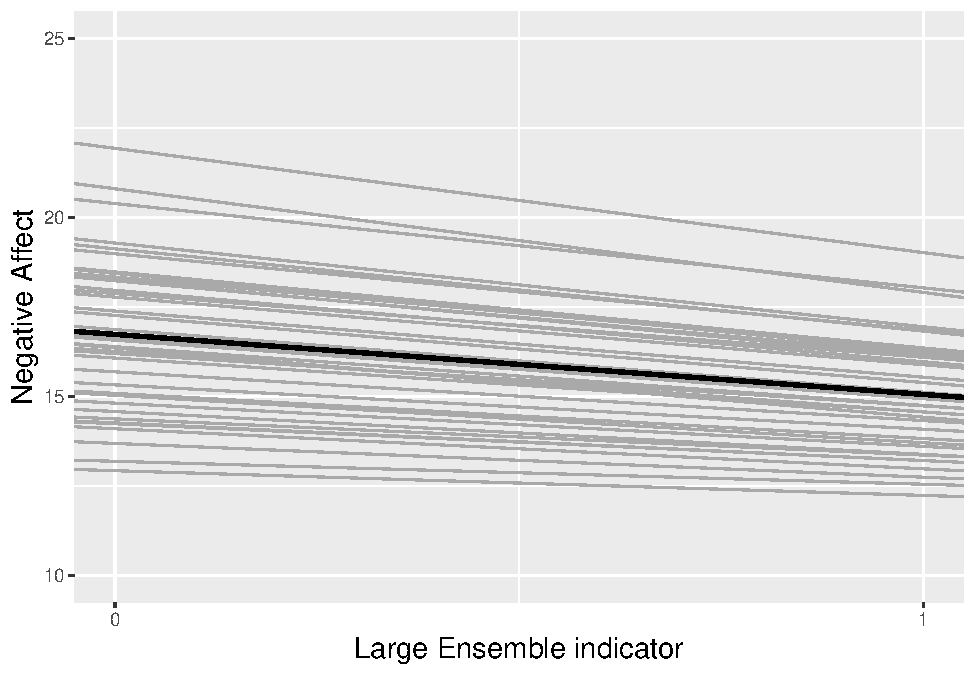
\includegraphics[width=0.6\linewidth]{bookdown-bysh_files/figure-latex/mli-spag1-1} 

}

\caption{The random slopes and intercepts model fitted to the music performance anxiety data.  Each gray line represents one subject, and the thicker black line represents the trend across all subjects.}\label{fig:mli-spag1}
\end{figure}

\begin{figure}

{\centering 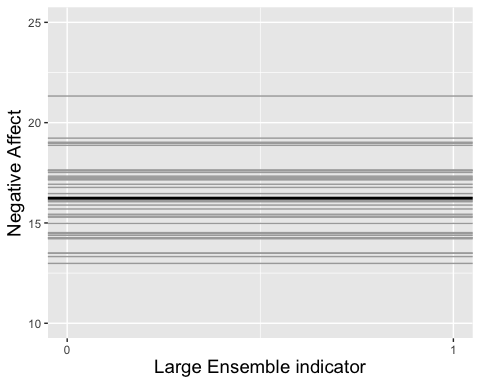
\includegraphics[width=0.6\linewidth]{bookdown-bysh_files/figure-latex/mli-spag0-1} 

}

\caption{The random intercepts model fitted to the music performance anxiety data.  Each gray line represents one subject, and the thicker black line represents the trend across all subjects.}\label{fig:mli-spag0}
\end{figure}

Figures \ref{fig:mli-spag1} and \ref{fig:mli-spag0} use \textbf{empirical Bayes estimates} \index{empirical Bayes estimates} for the intercepts (\(a_{i}\)) and slopes (\(b_{i}\)) of individual subjects. Empirical Bayes estimates are sometimes called ``shrinkage estimates'' since they combine individual-specific information with information from all subjects, thus ``shrinking'' the individual estimates toward the group averages. Empirical Bayes estimates are often used when a term such as \(a_{i}\) involves both fixed and random components; further detail can be found in \citet{Bryk2002} and \citet{Singer2003}.

\hypertarget{pseudoR2}{%
\subsection{\texorpdfstring{Pseudo \(R^2\) values}{Pseudo R\^{}2 values}}\label{pseudoR2}}

The estimated within-person variance \(\hat{\sigma}^2\) decreased by 3.1\% (from 22.5 to 21.8) from the unconditional means model, implying that only 3.1\% of within-person variability in performance anxiety scores can be explained by performance type. This calculation is considered a \textbf{pseudo R-square} \index{pseudo R-square} value:

\begin{equation*}
\textrm{Pseudo }R^2_{L1} = \frac{\hat{\sigma}^{2}(\textrm{Model A})-\hat{\sigma}^{2}(\textrm{Model B})}{\hat{\sigma}^{2}(\textrm{Model A})} = \frac{22.5-21.8}{22.5} = 0.031
\end{equation*}
Values of \(\hat{\sigma}_{u}^{2}\) and \(\hat{\sigma}_{v}^{2}\) from Model B cannot be compared to between-person variability from Model A, since the inclusion of performance type has changed the interpretation of these values, although they can provide important benchmarks for evaluating more complex Level Two predictions. Finally, \(\hat{\rho}_{uv}=-0.76\) indicates a strong negative relationship between a subject's performance anxiety before solos and small ensembles and their (typical) decrease in performance anxiety before large ensembles. As might be expected, subjects with higher levels of performance anxiety before solos and small ensembles tend to have smaller increases (or greater decreases) in performance anxiety before large ensembles; those with higher levels of performance anxiety before solos and small ensembles have more opportunity for decreases before large ensembles.

Pseudo \(R^2\) values are not universally reliable as measures of model performance. Because of the complexity of estimating fixed effects and variance components at various levels of a multilevel model, it is not unusual to encounter situations in which covariates in a Level Two equation for, say, the intercept remain constant (while other aspects of the model change), yet the associated pseudo \(R^2\) values differ or are negative. For this reason, pseudo \(R^2\) values in multilevel models should be interpreted cautiously.

\hypertarget{modelc}{%
\subsection{Adding a covariate at Level Two}\label{modelc}}

The initial two-level model described in section \ref{initialmodel} essentially expands upon the random slopes and intercepts model by adding a binary covariate for instrument played at Level Two. We will denote this as Model C:

\begin{itemize}
\item
  Level One:
  \begin{equation*}
  Y_{ij} = a_{i}+b_{i}\textrm{LargeEns}_{ij}+\epsilon_{ij}
  \end{equation*}
\item
  Level Two:
  \begin{align*}
  a_{i} & = \alpha_{0}+\alpha_{1}\textrm{Orch}_{i}+u_{i} \\
  b_{i} & = \beta_{0}+\beta_{1}\textrm{Orch}_{i}+v_{i},
  \end{align*}
  where \(\epsilon_{ij}\sim N(0,\sigma^2)\) and
\end{itemize}

\[ \left[ \begin{array}{c}
            u_{i} \\ v_{i}
          \end{array}  \right] \sim N \left( \left[
          \begin{array}{c}
            0 \\ 0
          \end{array} \right], \left[
          \begin{array}{cc}
            \sigma_{u}^{2} & \\
            \rho\sigma_{u}\sigma_{v} & \sigma_{v}^{2}
          \end{array} \right] \right). \]

We found that there are no highly significant fixed effects in Model C (other than the intercept). In particular, we have no significant evidence that musicians playing orchestral instruments reported different performance anxiety scores, on average, for solos and small ensembles than keyboardists and vocalists, no evidence of a difference in performance anxiety by performance type for keyboard players and vocalists, and no evidence of an instrument effect in difference between large ensembles and other types.

Since no terms were added at Level One when expanding from the random slopes and intercepts model (Model B), no discernable changes should occur in explained within-person variability (although small changes could occur due to numerical estimation procedures used in likelihood-based parameter estimates). However, Model C expanded Model B by using the instrument which a subject plays to model both intercepts and slopes at Level Two. We can use pseudo R-square values for both intercepts and slopes to evaluate the impact on between-person variability of adding instrument to Model B.

\begin{equation*}
\textrm{Pseudo }R^2_{L2_u} = \frac{\hat{\sigma}_{u}^{2}(\textrm{Model B})-\hat{\sigma}_{u}^{2}(\textrm{Model C})}{\hat{\sigma}_{u}^{2}(\textrm{Model B})} = \frac{6.33-5.66}{6.33} = 0.106
\end{equation*}

\begin{equation*}
\textrm{Pseudo }R^2_{L2_v} = \frac{\hat{\sigma}_{v}^{2}(\textrm{Model B})-\hat{\sigma}_{v}^{2}(\textrm{Model C})}{\hat{\sigma}_{v}^{2}(\textrm{Model B})} = \frac{0.74-0.45}{0.74} = 0.392
\end{equation*}
\(\textrm{Pseudo }R^2_{L2_u}\) describes the improvement in Model C over Model B in explaining subject-to-subject variability in intercepts, and \(\textrm{Pseudo }R^2_{L2_v}\) describes the improvement in Model C over Model B in explaining subject-to-subject variability in slopes. Thus, the addition of instrument at Level Two has decreased the between-person variability in mean performance anxiety before solos and small ensembles by 10.6\%, and it has decreased the between-person variability in the effect of large ensembles on performance anxiety by 39.2\%.

We could also run a ``random intercepts'' version of Model C, with no error term in the equation for the slope at Level Two (and thus no covariance between errors at Level Two as well):

\begin{itemize}
\item
  Level One:
  \begin{equation*}
  Y_{ij} = a_{i}+b_{i}\textrm{LargeEns}_{ij}+\epsilon_{ij}
  \end{equation*}
\item
  Level Two:
  \begin{align*}
  a_{i} & = \alpha_{0}+\alpha_{1}\textrm{Orch}_{i}+u_{i} \\
  b_{i} & = \beta_{0}+\beta_{1}\textrm{Orch}_{i},
  \end{align*}
  where \(\epsilon_{ij}\sim N(0,\sigma^2)\) and \(u_{i}\sim N(0,\sigma_{u}^{2})\).
\end{itemize}

The output below contains REML estimates of our 6 parameters from this simplified version of Model C (which we'll call Model C2):

\begin{Shaded}
\begin{Highlighting}[]
\CommentTok{#Model C2 (Run as random intercepts model)}
\NormalTok{model.c2 <-}\StringTok{ }\KeywordTok{lmer}\NormalTok{(na }\OperatorTok{~}\StringTok{ }\NormalTok{orch }\OperatorTok{+}\StringTok{ }\NormalTok{large }\OperatorTok{+}\StringTok{ }\NormalTok{orch}\OperatorTok{:}\NormalTok{large }\OperatorTok{+}
\StringTok{  }\NormalTok{(}\DecValTok{1}\OperatorTok{|}\NormalTok{id), }\DataTypeTok{data =}\NormalTok{ music)}
\end{Highlighting}
\end{Shaded}

\begin{verbatim}
##  Groups   Name        Variance Std.Dev.
##  id       (Intercept)  5.13    2.27    
##  Residual             21.88    4.68
\end{verbatim}

\begin{verbatim}
##  Number of Level Two groups =  37
\end{verbatim}

\begin{verbatim}
##             Estimate Std. Error t value
## (Intercept)  15.9026     0.6187  25.703
## orch          1.7100     0.9131   1.873
## large        -0.8918     0.8415  -1.060
## orch:large   -1.4650     1.0880  -1.347
\end{verbatim}

\begin{verbatim}
         df  AIC
model.c   8 3003
model.c2  6 2999
\end{verbatim}

\begin{verbatim}
         df  BIC
model.c   8 3037
model.c2  6 3025
\end{verbatim}

Note that parameter estimates for the remaining 6 fixed effects and variance components closely mirror the corresponding parameter estimates from Model C. In fact, removing the error term on the slope has improved (reduced) both the AIC and BIC measures of overall model performance. Instead of assuming that the large ensemble effects, after accounting for instrument played, vary by individual, we are assuming that large ensemble effect is fixed across subjects. It is not unusual to run a two-level model like this, with an error term on the intercept equation to account for subject-to-subject differences, but with no error terms on other Level Two equations unless there is an \emph{a priori} reason to allow effects to vary by subject or if the model performs better after building in those additional error terms.

\hypertarget{sec:modeld}{%
\section{Additional covariates: model comparison and interpretability}\label{sec:modeld}}

Recall that we are particularly interested in this study in Level Two covariates---those subject-specific variables that provide insight into why individuals react differently in anxiety-inducing situations. In section \ref{explore}, we saw evidence that subjects with higher baseline levels of negative emotionality tend to have higher performance anxiety levels prior to performances. Thus, in our next step in model building, we will add negative emotionality as a Level Two predictor to Model C. With this addition, our new model can be expressed as a system of Level One and Level Two models:

\begin{itemize}
\item
  Level One:
  \begin{equation*}
  Y_{ij} = a_{i}+b_{i}\textrm{LargeEns}_{ij}+\epsilon_{ij}
  \end{equation*}
\item
  Level Two:
  \begin{align*}
  a_{i} & = \alpha_{0}+\alpha_{1}\textrm{Orch}_{i}+\alpha_{2}\textrm{MPQnem}_{i}+u_{i} \\
  b_{i} & = \beta_{0}+\beta_{1}\textrm{Orch}_{i}+\beta_{2}\textrm{MPQnem}_{i}+v_{i},
  \end{align*}
  or as a composite model:
\end{itemize}

\begin{align*}
Y_{ij} & = [\alpha_{0}+\alpha_{1}\textrm{Orch}_{i}+\alpha_{2}\textrm{MPQnem}_{i}+\beta_{0}\textrm{LargeEns}_{ij} \\
 & \textrm{} + \beta_{1}\textrm{Orch}_{i}\textrm{LargeEns}_{ij}+\beta_{2}\textrm{MPQnem}_{i}\textrm{LargeEns}_{ij}] \\
 & \textrm{} + [u_{i}+v_{i}\textrm{LargeEns}_{ij}+\epsilon_{ij}]
\end{align*}
where error terms are defined as in Model C.

From the R output below, we see that, as our exploratory analyses suggested, subjects with higher baseline levels of stress reaction, alienation, and aggression (as measured by the MPQ negative emotionality scale) had significantly higher levels of performance anxiety before solos and small ensembles (t=3.893). They also had somewhat greater differences between large ensembles and other performance types, controlling for instrument (t=-0.575), although this interaction was not statistically significant.

\begin{Shaded}
\begin{Highlighting}[]
\CommentTok{# Model D (Add negative emotionality as second L2 covariate)}
\NormalTok{model.d <-}\StringTok{ }\KeywordTok{lmer}\NormalTok{(na }\OperatorTok{~}\StringTok{ }\NormalTok{orch }\OperatorTok{+}\StringTok{ }\NormalTok{mpqnem }\OperatorTok{+}\StringTok{ }\NormalTok{large }\OperatorTok{+}\StringTok{ }\NormalTok{orch}\OperatorTok{:}\NormalTok{large }\OperatorTok{+}\StringTok{ }
\StringTok{  }\NormalTok{mpqnem}\OperatorTok{:}\NormalTok{large }\OperatorTok{+}\StringTok{ }\NormalTok{(large }\OperatorTok{|}\StringTok{ }\NormalTok{id), }\DataTypeTok{data =}\NormalTok{ music)}
\end{Highlighting}
\end{Shaded}

\begin{verbatim}
##  Groups   Name        Variance Std.Dev. Corr 
##  id       (Intercept)  3.286   1.813         
##           large        0.557   0.746    -0.38
##  Residual             21.811   4.670
\end{verbatim}

\begin{verbatim}
##  Number of Level Two groups =  37
\end{verbatim}

\begin{verbatim}
##              Estimate Std. Error t value
## (Intercept)  11.56801    1.22057  9.4775
## orch          1.00069    0.81713  1.2246
## mpqnem        0.14823    0.03808  3.8925
## large        -0.28019    1.83412 -0.1528
## orch:large   -0.94927    1.10620 -0.8581
## mpqnem:large -0.03018    0.05246 -0.5753
\end{verbatim}

\hypertarget{interp:modeld}{%
\subsection{Interpretation of parameter estimates}\label{interp:modeld}}

Compared to Model C, the directions of the effects of instrument and performance type are consistent, but the effect sizes and levels of significance are reduced because of the relative importance of the negative emotionality term. Interpretations will also change slightly to acknowledge that we have controlled for a covariate. In addition, interpretations of fixed effects involving negative emotionality must acknowledge that this covariate is a continuous measure and not binary like instrument and performance type:

\begin{itemize}
\tightlist
\item
  \(\hat{\alpha}_{0} = 11.57\). The estimated mean performance anxiety for solos and small ensembles (\texttt{large=0}) is 11.57 for keyboard players and vocalists (\texttt{orch=0}) with negative emotionality of 0 at baseline (\texttt{mpqnem=0}). Since the minimum negative emotionality score in this study was 11, this interpretation, while technically correct, is not practically meaningful.
\item
  \(\hat{\alpha}_{1} = 1.00\). Orchestral instrument players have an estimated mean anxiety level before solos and small ensembles which is 1.00 point higher than keyboardists and vocalists, controlling for the effects of baseline negative emotionality.
\item
  \(\hat{\alpha}_{2} = 0.15\). A one point increase in baseline negative emotionality is associated with an estimated 0.15 mean increase in anxiety levels before solos and small ensembles, after controlling for instrument.
\item
  \(\hat{\beta}_{0} = -0.28\). Keyboard players and vocalists (\texttt{orch=0}) with baseline negative emotionality levels of 0 (\texttt{mpqnem=0}) have an estimated mean decrease in anxiety level of 0.28 points before large ensemble performances compared to other performance types.
\item
  \(\hat{\beta}_{1} = -0.95\). After accounting for baseline negative emotionality, orchestral instrument players have an estimated mean anxiety level before solos and small ensembles which is 1.00 point higher than keyboardists and vocalists, while the mean anxiety of orchestral players is only .05 points higher before large ensembles (a difference of .95 points).
\item
  \(\hat{\beta}_{2} = -0.03\). After accounting for instrument, a one point increase in baseline negative emotionality is associated with an estimated 0.15 mean increase in anxiety levels before solos and small ensembles, but only an estimated 0.12 increase before large ensembles (a difference of .03 points).
\end{itemize}

Some of the detail in these parameter interpretations can be tricky---describing interaction terms, deciding if a covariate must be fixed at 0 or merely held constant, etc. Often it helps to write out models for special cases to isolate the effects of specific fixed effects. We will consider a few parameter estimates from above and see why the interpretations are written as they are.

\begin{itemize}
\tightlist
\item
  \(\hat{\alpha}_{1}\). For solos and small ensembles (\texttt{LargeEns=0}), the following equations describe the fixed effects portion of the composite model for negative affect score for vocalists and keyboardsists (\texttt{Orch=0}) and orchestral instrumentalists (\texttt{Orch=1}):
\end{itemize}

\begin{align*}
\textrm{Orch}=0: & \\
Y_{ij} & = \alpha_{0}+\alpha_{2}\textrm{MPQnem}_{i} \\
\textrm{Orch}=1: & \\
Y_{ij} & = (\alpha_{0}+\alpha_{1})+\alpha_{2}\textrm{MPQnem}_{i}
\end{align*}
Regardless of the subjects' baseline negative emotionality (\texttt{MPQnem}), \(\hat{\alpha}_{1}\) represents the estimated difference in performance anxiety between those playing orchestral instruments and others. This interpretation, however, only holds for solos and small ensembles. For large ensembles, the difference between those playing orchestral instruments and others is actually given by \(\hat{\alpha}_{1}+\hat{\beta}_{1}\), holding \texttt{MPQnem} constant (Show!).

\begin{itemize}
\tightlist
\item
  \(\hat{\beta}_{0}\). Because \texttt{LargeEns} interacts with both \texttt{Orch} and \texttt{MPQnem} in Model C, \(\hat{\beta}_{0}\) only describes the estimated difference between large ensembles and other performance types when both \texttt{Orch=0} and \texttt{MPQnem=0}, thus removing the effects of the interaction terms. If, for instance, \texttt{Orch=1} and \texttt{MPQnem=20}, then the difference between large ensembles and other performance types is given by \(\hat{\beta}_{0}+\hat{\beta}_{1}+20\hat{\beta}_{2}\).
\item
  \(\hat{\beta}_{1}\). As with \(\hat{\alpha}_{1}\), we consider equations describing the fixed effects portion of the composite model for negative affect score for vocalists and keyboardsists (\texttt{Orch=0}) and orchestral instrumentalists (\texttt{Orch=1}), except here we leave \emph{LargeEns} as an unknown rather than restricting the model to solos and small ensembles:
\end{itemize}

\begin{align*}
\textrm{Orch}=0: & & \\
Y_{ij} & = \alpha_{0}+\alpha_{2}\textrm{MPQnem}_{i}+\beta_{0}\textrm{LargeEns}_{ij} \\
 & \textrm{} +\beta_{2}\textrm{MPQnem}_{i}\textrm{LargeEns}_{ij} \\
\textrm{Orch}=1: & \\
Y_{ij} & = (\alpha_{0}+\alpha_{1})+\alpha_{2}\textrm{MPQnem}_{i}+(\beta_{0}+\beta_{1})\textrm{LargeEns}_{ij} \\
 & \textrm{} +\beta_{2}\textrm{MPQnem}_{i}\textrm{LargeEns}_{ij}
\end{align*}
As long as baseline negative emotionality is held constant (at any level, not just 0), then \(\hat{\beta}_{1}\) represents the estimated difference in the large ensemble effect between those playing orchestral instruments and others.

\hypertarget{compare:modeld}{%
\subsection{Model comparisons}\label{compare:modeld}}

At this point, we might ask: do the two extra fixed effects terms in Model D provide a significant improvement over Model C? Nested models such as these can be tested using a \textbf{likelihood ratio test} \index{likelihood ratio test (LRT)} (drop in deviance test) \index{drop-in-deviance test}, as we've used in Sections \ref{sec-Devtocompare} and \ref{sec-logisticInf} with certain generalized linear models. Since we are comparing models nested in their fixed effects, we use full maximum likelihood methods to estimate model parameters, as discussed in section \ref{multileveltechnical}. As expected, the likelihood is larger (and the log-likelihood is less negative) under the larger model (Model D); our test statistic (14.734) is then -2 times the difference in log-likelihood between Models C and D. Comparing the test statistic to a chi-square distribution with 2 degrees of freedom (signifying the number of additional terms in Model D), we obtain a p-value of .0006. Thus, Model D significantly outperforms Model C.

\begin{Shaded}
\begin{Highlighting}[]
\CommentTok{# anova() automatically uses ML for LRT tests}
\NormalTok{drop_in_dev <-}\StringTok{ }\KeywordTok{anova}\NormalTok{(model.d, model.c, }\DataTypeTok{test =} \StringTok{"Chisq"}\NormalTok{)}
\end{Highlighting}
\end{Shaded}

\begin{verbatim}
        npar  AIC  BIC logLik  dev Chisq Df      pval
model.c    8 3007 3041  -1496 2991    NA NA        NA
model.d   10 2996 3039  -1488 2976 14.73  2 0.0006319
\end{verbatim}

Two models, whether they are nested or not, can be compared using AIC and BIC measures, which were first seen in Chapter \ref{ch-MLRreview} and later used in evaluating generalized linear models. In this case, the AIC clearly favors Model D (2996.7) over Model C (3007.3), whereas the BIC favors Model D (3038.8) only slightly over Model C (3041.0) since the BIC imposes a stiffer penalty on additional terms and additional model complexity. However, the likelihood ratio test is a more reliable method for comparing nested models.

Finally, we note that Model D could be further improved by dropping the negative emotionality by large ensemble interaction term. Not only is the t-value (-0.575) associated with this term of low magnitude, but a likelihood ratio test comparing Model D to a model without \texttt{mpqnem:large} produces an insignificant p-value of 0.5534.

\begin{Shaded}
\begin{Highlighting}[]
\NormalTok{drop_in_dev <-}\StringTok{ }\KeywordTok{anova}\NormalTok{(model.d, model.d1, }\DataTypeTok{test =} \StringTok{"Chisq"}\NormalTok{)}
\end{Highlighting}
\end{Shaded}

\begin{verbatim}
         npar  AIC  BIC logLik  dev  Chisq Df   pval
model.d1    9 2995 3033  -1488 2977     NA NA     NA
model.d    10 2996 3039  -1488 2976 0.3513  1 0.5534
\end{verbatim}

\hypertarget{sec:modele}{%
\section{Center covariates}\label{sec:modele}}

As we observed above, the addition of baseline negative emotionality in Model D did not always produce sensible interpretations of fixed effects. It makes no sense to draw conclusions about performance anxiety levels for subjects with MPQNEM scores of 0 at baseline (as in \(\hat{\beta}_{0}\)), since the minimum NEM composite score among subjects in this study was 11. In order to produce more meaningful interpretations of parameter estimates and often more stable parameter estimates, it is often wise to \textbf{center} \index{centering} explanatory variables. Centering involves subtracting a fixed value from each observation, where the fixed value represents a meaningful anchor value (e.g., last grade completed is 12; GPA is 3.0). Often, when there's no pre-defined anchor value, the mean is used to represent a typical case. With this in mind, we can create a new variable

\begin{align*}
\textrm{centeredbaselineNEM} & = \textrm{cmpqnem} \\
 & = \textrm{mpqnem - mean(mpqnem)} \\
 & = \textrm{mpqnem} - 31.63
\end{align*}
and replace baseline NEM in Model D with its centered version to create Model E:

\begin{Shaded}
\begin{Highlighting}[]
\CommentTok{# Model E (Center baseline NEM in Model D)}
\NormalTok{model.e <-}\StringTok{ }\KeywordTok{lmer}\NormalTok{(na }\OperatorTok{~}\StringTok{ }\NormalTok{orch }\OperatorTok{+}\StringTok{ }\NormalTok{cmpqnem }\OperatorTok{+}\StringTok{ }\NormalTok{large }\OperatorTok{+}\StringTok{ }\NormalTok{orch}\OperatorTok{:}\NormalTok{large }\OperatorTok{+}\StringTok{ }
\StringTok{  }\NormalTok{cmpqnem}\OperatorTok{:}\NormalTok{large }\OperatorTok{+}\StringTok{ }\NormalTok{(large }\OperatorTok{|}\StringTok{ }\NormalTok{id), }\DataTypeTok{REML =}\NormalTok{ T, }\DataTypeTok{data =}\NormalTok{ music)}
\end{Highlighting}
\end{Shaded}

\begin{verbatim}
##  Groups   Name        Variance Std.Dev. Corr 
##  id       (Intercept)  3.286   1.813         
##           large        0.557   0.746    -0.38
##  Residual             21.811   4.670
\end{verbatim}

\begin{verbatim}
##  Number of Level Two groups =  37
\end{verbatim}

\begin{verbatim}
##               Estimate Std. Error t value
## (Intercept)   16.25679    0.54756 29.6893
## orch           1.00069    0.81713  1.2246
## cmpqnem        0.14823    0.03808  3.8925
## large         -1.23484    0.84320 -1.4645
## orch:large    -0.94927    1.10620 -0.8581
## cmpqnem:large -0.03018    0.05246 -0.5753
\end{verbatim}

As you compare Model D to Model E, you should notice that only two things change -- \(\hat{\alpha}_{0}\) and \(\hat{\beta}_{0}\). All other parameter estimates---both fixed effects and variance components---remain identical; the basic model is essentially unchanged as well as the amount of variability in anxiety levels explained by the model. \(\hat{\alpha}_{0}\) and \(\hat{\beta}_{0}\) are the only two parameter estimates whose interpretations in Model D refer to a specific level of baseline NEM. In fact, the interpretations that held true where \texttt{NEM=0} (which isn't possible) now hold true for \texttt{cmpqnem=0} or when NEM is at its average value of 31.63, which is possible and quite meaningful. Now, parameter estimates using centered baseline NEM in Model E change in value from Model D and produce more useful interpretations:

\begin{itemize}
\tightlist
\item
  \(\hat{\alpha}_{0} = 16.26\). The estimated mean performance anxiety for solos and small ensembles (\texttt{large=0}) is 16.26 for keyboard players and vocalists (\texttt{orch=0}) with an average level of negative emotionality at baseline (\texttt{mpqnem=31.63}).
\item
  \(\hat{\beta}_{0} = -1.23\). Keyboard players and vocalists (\texttt{orch=0}) with an average level of baseline negative emotionality levels (\texttt{mpqnem=31.63}) have an estimated mean decrease in anxiety level of 1.23 points before large ensemble performances compared to other performance types.
\end{itemize}

\hypertarget{modelf}{%
\section{A potential final model for music performance anxiety}\label{modelf}}

We now begin iterating toward a ``final model'' for these data, on which we will base conclusions. Typical features of a ``final multilevel model'' \index{multilevel model} include:

\begin{itemize}
\tightlist
\item
  fixed effects allow one to address primary research questions
\item
  fixed effects control for important covariates at all levels
\item
  potential interactions have been investigated
\item
  variables are centered where interpretations can be enhanced
\item
  important variance components have been included
\item
  unnecessary terms have been removed
\item
  the model tells a ``persuasive story parsimoniously''
\end{itemize}

Although the process of reporting and writing up research results often demands the selection of a sensible final model, it's important to realize that (a) statisticians typically will examine and consider an entire taxonomy of models when formulating conclusions, and (b) different statisticians sometimes select different models as their ``final model'' for the same set of data. Choice of a ``final model'' depends on many factors, such as primary research questions, purpose of modeling, tradeoff between parsimony and quality of fitted model, underlying assumptions, etc. So you should be able to defend any final model you select, but you should not feel pressured to find the one and only ``correct model'', although most good models will lead to similar conclusions.

As we've done in previous sections, we can use (a) t-statistics for individual fixed effects when considering adding a single term to an existing model, (b) likelihood ratio tests for comparing nested models which differ by more than one parameter, and (c) model performance measures such as AIC and BIC to compare non-nested models. Below we offer one possible final model for this data---Model F:

\begin{itemize}
\tightlist
\item
  Level One:
\end{itemize}

\begin{equation*}
Y_{ij} = a_{i}+b_{i}\textrm{previous}_{ij}+c_{i}\textrm{students}_{ij}+
d_{i}\textrm{juried}_{ij}+e_{i}\textrm{public}_{ij}+f_{i}\textrm{solo}_{ij}+\epsilon_{ij}
\end{equation*}

\begin{itemize}
\tightlist
\item
  Level Two:
\end{itemize}

\begin{align*}
a_{i} & = \alpha_{0}+\alpha_{1}\textrm{mpqpem}_{i}+\alpha_{2}\textrm{mpqab}_{i} + \alpha_{3}\textrm{orch}_{i}+\alpha_{4}\textrm{mpqnem}_{i}+u_{i} \\
b_{i} & = \beta_{0}+v_{i}, \\
c_{i} & = \gamma_{0}+w_{i}, \\
d_{i} & = \delta_{0}+x_{i}, \\
e_{i} & = \varepsilon_{0}+y_{i}, \\
f_{i} & = \zeta_{0}+\zeta_{1}\textrm{mpqnem}_{i}+z_{i},
\end{align*}
where \texttt{previous} is the number of previous diary entries filled out by that individual (\texttt{diary-1}); \texttt{students}, \texttt{juried}, and \texttt{public} are indicator variables created from the \texttt{audience} categorical variable (so that ``Instructor'' is the reference level in this model); and, \texttt{solo} is 1 if the performance was a solo and 0 if the performance was either a small or large ensemble.

In addition, we assume the following variance-covariance structure at Level Two:

\[ \left[ \begin{array}{c}
            u_{i} \\ v_{i} \\ w_{i} \\ x_{i} \\ y_{i} \\ z_{i}
          \end{array}  \right] \sim N \left( \left[
          \begin{array}{c}
            0 \\ 0 \\ 0 \\ 0 \\ 0 \\ 0
          \end{array} \right], \left[
          \begin{array}{cccccc}
            \sigma_{u}^{2} & & & & & \\
            \sigma_{uv} & \sigma_{v}^{2} & & & & \\
            \sigma_{uw} & \sigma_{vw} & \sigma_{w}^{2} & & & \\
            \sigma_{ux} & \sigma_{vx} & \sigma_{wx} & \sigma_{x}^{2} & & \\
            \sigma_{uy} & \sigma_{vy} & \sigma_{wy} & \sigma_{xy} & \sigma_{y}^{2} & \\
            \sigma_{uz} & \sigma_{vz} & \sigma_{wz} & \sigma_{xz} & \sigma_{yz} & \sigma_{z}^{2}
          \end{array} \right] \right). \]

Being able to write out these mammoth variance-covariance matrices is less important than recognizing the number of variance components that must be estimated by our intended model. In this case, we must use likelihood-based methods to obtain estimates for 6 variance terms and 15 correlation terms at Level Two, along with 1 variance term at Level One. Note that the number of correlation terms is equal to the number of unique pairs among Level Two random effects. In later sections we will consider ways to reduce the number of variance components in cases where the number of terms is exploding or the statistical software is struggling to simultaneously find estimates for all model parameters to maximize the likelihood function.

From the signs of fixed effects estimates in the R output below, we see that performance anxiety is higher when a musician is performing in front of students, a jury, or the general public rather than their instructor, and it is lower for each additional diary the musician previously filled out. In addition, musicians with lower levels of positive emotionality and higher levels of absorption tend to experience greater performance anxiety, and those who play orchestral instruments experience more performance anxiety than those who play keyboards or sing. Addressing the researchers' primary hypothesis, after controlling for all these factors, we have significant evidence that musicians with higher levels of negative emotionality experience higher levels of performance anxiety, and that this association is even more pronounced when musicians are performing solos rather than as part of an ensemble group.

Here are how a couple of key fixed effects would be interpreted in this final model:

\begin{itemize}
\tightlist
\item
  \(\hat{\alpha}_{4} = 0.11\). A one point increase in baseline level of negative emotionality is associated with an estimated 0.11 mean increase in performance anxiety for musicians performing in an ensemble group (\texttt{solo=0}), after controlling for previous diary entries, audience, positive emotionality, absorption, and instrument.
\item
  \(\hat{\zeta}_{1} = 0.08\). When musicians play solos, a one point increase in baseline level of negative emotionality is associated with an estimated 0.19 mean increase in performance anxiety, 0.08 points (73\%) higher than musicians playing in ensemble groups, controlling for the effects of previous diary entries, audience, positive emotionality, absorption, and instrument.
\end{itemize}

\begin{Shaded}
\begin{Highlighting}[]
\CommentTok{# Model F (One - of many - reasonable final models)}
\NormalTok{model.f <-}\StringTok{ }\KeywordTok{lmer}\NormalTok{(na }\OperatorTok{~}\StringTok{ }\NormalTok{previous }\OperatorTok{+}\StringTok{ }\NormalTok{students }\OperatorTok{+}\StringTok{ }\NormalTok{juried }\OperatorTok{+}\StringTok{ }
\StringTok{    }\NormalTok{public }\OperatorTok{+}\StringTok{ }\NormalTok{solo }\OperatorTok{+}\StringTok{ }\NormalTok{mpqpem }\OperatorTok{+}\StringTok{ }\NormalTok{mpqab }\OperatorTok{+}\StringTok{ }\NormalTok{orch }\OperatorTok{+}\StringTok{ }\NormalTok{mpqnem }\OperatorTok{+}\StringTok{ }
\StringTok{    }\NormalTok{mpqnem}\OperatorTok{:}\NormalTok{solo }\OperatorTok{+}\StringTok{ }\NormalTok{(previous }\OperatorTok{+}\StringTok{ }\NormalTok{students }\OperatorTok{+}\StringTok{ }\NormalTok{juried }\OperatorTok{+}\StringTok{ }
\StringTok{    }\NormalTok{public }\OperatorTok{+}\StringTok{ }\NormalTok{solo }\OperatorTok{|}\StringTok{ }\NormalTok{id), }\DataTypeTok{REML =}\NormalTok{ T, }\DataTypeTok{data =}\NormalTok{ music)}
\end{Highlighting}
\end{Shaded}

\begin{verbatim}
##  Groups   Name        Variance Std.Dev. Corr       
##  id       (Intercept) 14.4802  3.805               
##           previous     0.0707  0.266    -0.65      
##           students     8.2151  2.866    -0.63  0.00
##           juried      18.3177  4.280    -0.64 -0.12
##           public      12.8094  3.579    -0.83  0.33
##           solo         0.7665  0.876    -0.67  0.47
##  Residual             15.2844  3.910               
##                   
##                   
##                   
##                   
##   0.84            
##   0.66  0.58      
##   0.49  0.21  0.90
## 
\end{verbatim}

\begin{verbatim}
##  Number of Level Two groups =  37
\end{verbatim}

\begin{verbatim}
##             Estimate Std. Error t value
## (Intercept)  8.36883    1.91369  4.3731
## previous    -0.14303    0.06247 -2.2895
## students     3.61115    0.76796  4.7022
## juried       4.07332    1.03130  3.9497
## public       3.06453    0.89274  3.4327
## solo         0.51647    1.39635  0.3699
## mpqpem      -0.08312    0.02408 -3.4524
## mpqab        0.20377    0.04740  4.2986
## orch         1.53138    0.58384  2.6230
## mpqnem       0.11465    0.03591  3.1930
## solo:mpqnem  0.08296    0.04158  1.9951
\end{verbatim}

\hypertarget{multinecessary}{%
\section{Modeling the multilevel structure: is it really necessary?}\label{multinecessary}}

Before going too much further, we should really consider if this multilevel structure has gained us anything over linear least squares regression \index{linear least squares regression (LLSR)}. Sure, multilevel modeling \index{multilevel model} seems more faithful to the inherent structure of the data---performances from the same musician should be more highly correlated than performances from different musicians---but do our conclusions change in a practical sense? Some authors have expressed doubts. For instance Robert Bickel, in his 2007 book, states, ``When comparing OLS and multilevel regression results, we may find that differences among coefficient values are inconsequential, and tests of significance may lead to the same decisions. A great deal of effort seems to have yielded precious little gain'' \citep{Bickel2007}. Others, especially economists, advocate simply accounting for the effect of different Level Two observational units (like \texttt{musicians}) with a sequence of indicator variables for those observational units. We contend that (1) fitting multilevel models is a small extension of LLSR regression that is not that difficult to conceptualize and fit, especially with the software available today, and (2) using multilevel models to remain faithful to the data structure \emph{can} lead to different coefficient estimates and \emph{often} leads to different (and larger) standard error estimates and thus smaller test statistics. Hopefully you've seen evidence of (1) in this chapter already; the rest of this section introduces two small examples to help illustrate (2).

\begin{figure}

{\centering 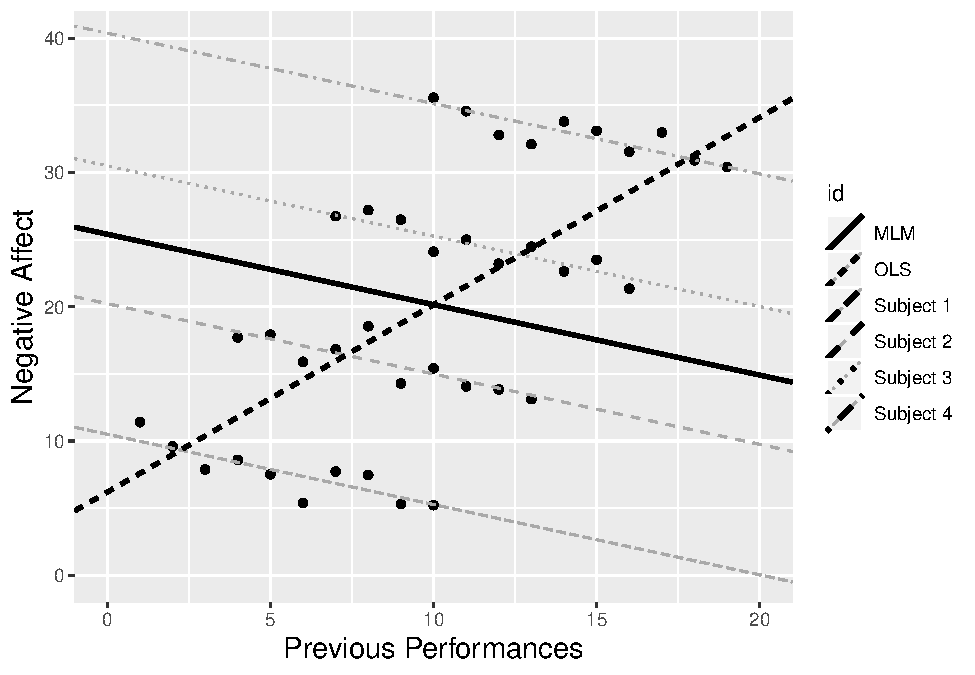
\includegraphics[width=0.6\linewidth]{bookdown-bysh_files/figure-latex/mli-spag2-1} 

}

\caption{Hypothetical data from 4 subjects relating number of previous performances to negative affect.  The solid black line depicts the overall relationship between previous performances and negative affect as determined by a multilevel model, while the dashed black line depicts the overall relationship as determined by an LLSR regression model.}\label{fig:mli-spag2}
\end{figure}

Figure \ref{fig:mli-spag2} is based on a synthetic data set containing 10 observations from each of 4 subjects. For each subject, the relationship between previous performances and negative affect is linear and negative, with slope approximately -0.5 but different intercepts. The multilevel model (a random intercepts model as described in section \ref{modelb}) shows an overall relationship (the solid black line) that's consistent with the individual subjects---slope around -0.5 with an intercept that appears to average the 4 subjects. Fitting a LLSR model, however, produces an overall relationship (the dashed black line) that is strongly positive. In this case, by naively fitting the 40 observations as if they were all independent and ignoring subject effects, the LLSR analysis has gotten the estimated slope of the overall relationship backwards, producing a continuous data version of Simpson's Paradox.



\begin{figure}

{\centering 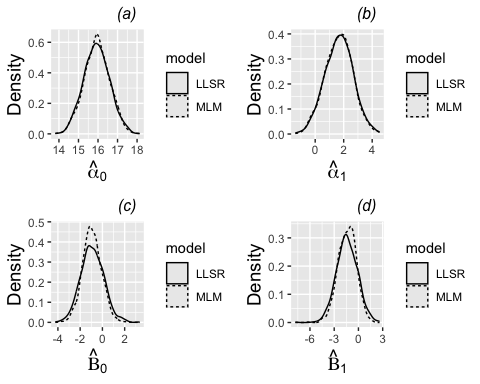
\includegraphics[width=0.6\linewidth]{bookdown-bysh_files/figure-latex/mli-density1-1} 

}

\caption{Density plots of parameter estimates for the four fixed effects of Model C under both a multilevel model and linear least squares regression. 1000 sets of simulated data for the 37 subjects in our study were produced using estimated fixed and random effects from Model C. For each set of simulated data, estimates of (a) \(\alpha_{0}\), (b) \(\alpha_{1}\), (c) \(\beta_{0}\), and (d) \(\beta_{1}\) were obtained using both a multilevel and an LLSR model. Each plot then shows a density plot for the 1000 estimates of the corresponding fixed effect using multilevel modeling vs.~a similar density plot for the 1000 estimates using LLSR.}\label{fig:mli-density1}
\end{figure}



\begin{figure}

{\centering 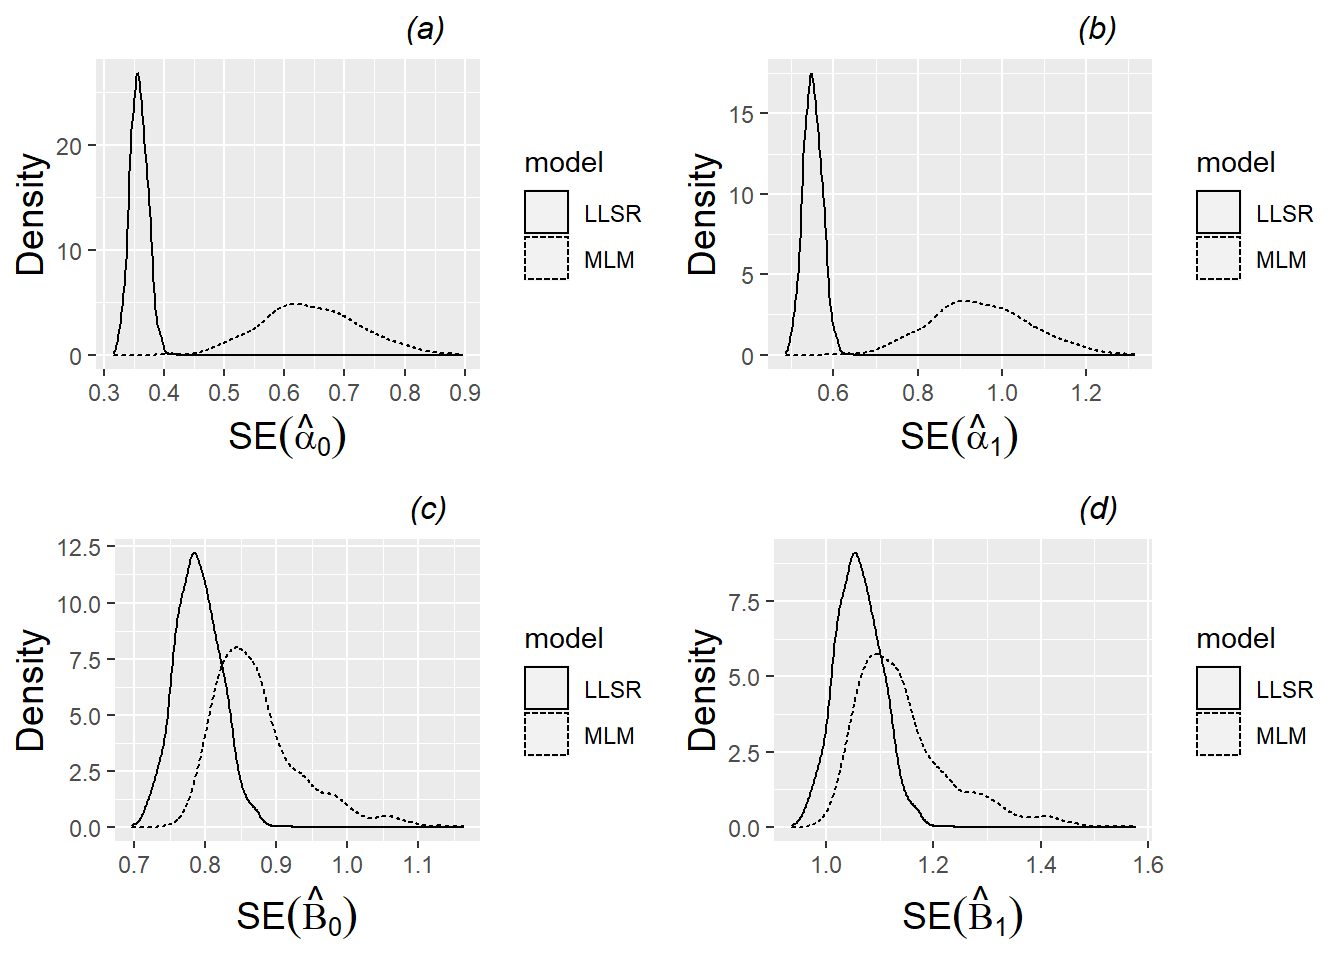
\includegraphics[width=0.6\linewidth]{bookdown-bysh_files/figure-latex/mli-density2-1} 

}

\caption{Density plots of standard errors of parameter estimates for the four fixed effects of Model C under both a multilevel model and linear least squares regression. 1000 sets of simulated data for the 37 subjects in our study were produced using estimated fixed and random effects from Model C. For each set of simulated data, estimates of (a) SE(\(\alpha_{0}\)), (b) SE(\(\alpha_{1}\)), (c) SE(\(\beta_{0}\)), and (d) SE(\(\beta_{1}\)) were obtained using both a multilevel and an LLSR model. Each plot then shows a density plot for the 1000 estimates of the corresponding standard error term using multilevel modeling vs.~a similar density plot for the 1000 estimates using LLSR.}\label{fig:mli-density2}
\end{figure}

Our second example is based upon Model C from section \ref{modelc}, with single binary predictors at both Level One and Level Two. Using the estimated fixed effects coefficients and variance components from random effects produced in Model C, we generated 1000 sets of simulated data. Each set of simulated data contained 497 observations from 37 subjects just like the original data, with relationships between negative affect and large ensembles and orchestral instruments (along with associated variability) governed by the estimated parameters from Model C. Each set of simulated data was used to fit both a multilevel model and a linear least squares regression model, and the estimated fixed effects (\(\hat{\alpha}_{0}\), \(\hat{\alpha}_{1}\), \(\hat{\beta}_{0}\), and \(\hat{\beta}_{1}\)) and their standard errors were saved. Figure \ref{fig:mli-density1} shows density plots comparing the 1000 estimated values for each fixed effect from the two modeling approaches; in general, estimates from multilevel modeling and LLSR tend to agree pretty well, without noticeable bias. Based on coefficient estimates alone, there appears to be no reason to favor multilevel modeling over LLSR in this example, but Figure \ref{fig:mli-density2} tells a different story. Figure \ref{fig:mli-density2} shows density plots comparing the 1000 estimated standard errors associated with each fixed effect from the two modeling approaches; in general, standard errors are markedly larger with multilevel modeling than LLSR. This is not unusual, since LLSR assumes all 497 observations are independent while multilevel modeling acknowledges that, with correlated data within subject, there are fewer than 497 independent pieces of data. Therefore, linear least squares regression can overstate precision, producing t-statistics for each fixed effect that tend to be larger than they should be; the number of significant results in LLSR are then too great and not reflective of the true structure of the data.

\hypertarget{notesr8}{%
\section{Notes on Using R (Optional)}\label{notesr8}}

Initial examination of the data for Case Study \ref{cs:music} shows a couple of features that must be noted. First, there are 37 unique study participants, but they are not numbered successively from 1 to 43. The majority of participants filled out 15 diaries, but several filled out fewer (with a minimum of 2); as with participant IDs, diary numbers within participant are not always successively numbered. Finally, missing data is not an issue in this data set, since researchers had already removed participants with only 1 diary entry and performances for which the type was not recorded (of which there were 11).

The R code below runs the initial multilevel model \index{multilevel model} in section \ref{initialmodel}. Multilevel model notation in R is based on the composite model formulation. Here, the response variable is \texttt{na}, while \texttt{orch}, \texttt{large}, and \texttt{orch:large} represent the fixed effects \(\alpha_{1}\), \(\beta_{0}\), and \(\beta_{1}\), along with the intercept \(\alpha_{0}\) which is included automatically. Note that a colon is used to denote an interaction between two variables. Error terms and their associated variance components are specified in \texttt{(large\textbar{}id)}, which is equivalent to \texttt{(1+large\textbar{}id)}. This specifies two error terms at Level Two (the \texttt{id} level): one corresponding to the intercept (\(u_{i}\)) and one corresponding to the large ensemble effect (\(v_{i}\)); the multilevel model will then automatically include a variance for each error term in addition to the covariance between the two error terms. A variance associated with a Level One error term is also automatically included in the multilevel model. Note that there are ways to override the automatic inclusion of certain variance components; for example, \texttt{(0+large\textbar{}id)} would not include an error term for the intercept (and therefore no covariance term at Level Two either).

\begin{Shaded}
\begin{Highlighting}[]
\NormalTok{model0 <-}\StringTok{ }\KeywordTok{lmer}\NormalTok{(na }\OperatorTok{~}\StringTok{ }\NormalTok{orch }\OperatorTok{+}\StringTok{ }\NormalTok{large }\OperatorTok{+}\StringTok{ }\NormalTok{orch}\OperatorTok{:}\NormalTok{large }\OperatorTok{+}
\StringTok{  }\NormalTok{(large }\OperatorTok{|}\StringTok{ }\NormalTok{id), }\DataTypeTok{REML =}\NormalTok{ T, }\DataTypeTok{data =}\NormalTok{ music)}
\KeywordTok{summary}\NormalTok{(model0)}
\end{Highlighting}
\end{Shaded}

\hypertarget{exercises}{%
\section{Exercises}\label{exercises}}

\hypertarget{conceptual-exercises}{%
\subsection{Conceptual Exercises}\label{conceptual-exercises}}

\begin{enumerate}
\def\labelenumi{\arabic{enumi}.}
\item
  \textbf{Housing Prices.} \citet{Brown2004} describe ``A Hierarchical Linear Model Approach for Assessing the Effects of House and Neighborhood Characteristics on Housing Prices''. Based on the title of their paper: (a) give the observational units at Level One and Level Two, and (b) list potential explanatory variables at both Level One and Level Two.
\item
  In the preceding problem, why can't we assume all houses in the data set are independent? What would be the potential implications to our analysis of assuming independence among houses?
\item
  In the preceding problem, for each of the following sets of predictors: (a) write out the two-level model for predicting housing prices, (b) write out the corresponding composite model, and (c) determine how many model parameters (fixed effects and variance components) must be estimated.

  \begin{itemize}
  \tightlist
  \item
    Square footage, number of bedrooms
  \item
    Median neighborhood income, rating of neighborhood schools
  \item
    Square footage, number of bedrooms, age of house, median neighborhood housing price
  \item
    Square footage, median neighborhood income, rating of neighborhood schools, median neighborhood housing price
  \end{itemize}
\item
  \textbf{Music Performance Anxiety.} Describe a situation in which the two plots in Figure \ref{fig:mli-boxmat1} might tell different stories.
\item
  Explain the difference between \(a_{i}\) in Equation \eqref{eq:level2s0} and \(\hat{a}_{i}\) in Equation \eqref{eq:level2s0hat}.
\item
  Why is the contour plot for multivariate normal density in Figure \ref{fig:contour-boundary} (b) tilted from southwest to northeast, but the contour plot in Figure \ref{fig:contour-boundary} (a) is not tilted?
\item
  In Table \ref{tab:table3chp8}, note that the standard errors associated with estimated coefficients under independence are lower than standard errors under alternative analysis methods. Why is that often the case?
\item
  Why is Model A (Section \ref{modela8}) sometimes called the ``unconditional means model''? Why is it also sometimes called the ``random intercepts model''? Are these two labels consistent with each other?
\item
  Consider adding an indicator variable in Model B (Section \ref{randomslopeandint}) for Small Ensemble performances.

  \begin{itemize}
  \tightlist
  \item
    Write out the two-level model for performance anxiety,
  \item
    Write out the corresponding composite model,
  \item
    Determine how many model parameters (fixed effects and variance components) must be estimated, and
  \item
    Explain how the interpretation for the coefficient in front of Large Ensembles would change.
  \end{itemize}
\item
  Give a short rule in your own words describing when an interpretation of an estimated coefficient should ``hold constant'' another covariate or ``set to 0'' that covariate (see Section \ref{interp:modeld}).
\item
  The interpretation of \(\hat{\alpha}_{1}\) in Section \ref{interp:modeld} claims that ``This interpretation, however, only holds for solos and small ensembles. For large ensembles, the difference between those playing orchestral instruments and others is actually given by \(\hat{\alpha}_{1}+\hat{\beta}_{1}\), holding MPQNEM constant.'' Show that this claim is true.
\item
  Explain how the interpretations of the following parameter estimates change (or don't change) as we change our model:

  \begin{itemize}
  \tightlist
  \item
    \(\hat{\alpha}_{0}\) from Model A to B to C to D to E
  \item
    \(\hat{\beta}_{1}\) from Model B to C to D to E
  \item
    \(\hat{\alpha}_{1}\) from Model C to D to E
  \item
    \(\hat{\beta}_{1}\) from Model C to D to E
  \item
    \(\hat{\sigma}_{u}\) from Model A to B to C to D to E
  \item
    \(\hat{\sigma}_{v}\) from Model B to C to D to E
  \end{itemize}
\item
  When moving from Model B to Model C in Section \ref{modelc}, \(\hat{\sigma}_{u}^{2}\) increases slightly. Why might this have occurred?
\item
  Interpret other estimated parameters from Model F beyond those interpreted in Section \ref{modelf}: \(\hat{\alpha}_{0}\), \(\hat{\alpha}_{2}\), \(\hat{\alpha}_{3}\), \(\hat{\beta}_{0}\), \(\hat{\gamma}_{0}\), \(\hat{\zeta}_{0}\), \(\hat{\rho}_{wx}\), \(\hat{\sigma}^{2}\), \(\hat{\sigma}_{u}^{2}\), and \(\hat{\sigma}_{z}^{2}\).
\item
  Explain Figure \ref{fig:mli-spag2} in your own words. Why would LLSR produce a misleading analysis in this case, but multilevel models would not?
\item
  Summarize Figures \ref{fig:mli-density1} and \ref{fig:mli-density2} in your own words.
\end{enumerate}

\hypertarget{guided-exercise}{%
\subsection{Guided Exercise}\label{guided-exercise}}

\begin{enumerate}
\def\labelenumi{\arabic{enumi}.}
\item
  \textbf{Music Performance Joy.} In this chapter, we studied models for predicting music performance anxiety, as measured by the negative affect scale from the PANAS instrument. Now we will examine models for predicting the happiness of musicians prior to performances, as measured by the positive affect scale from the PANAS instrument.

  To begin, run the following models:

  \begin{itemize}
  \tightlist
  \item
    Model A = unconditional means model
  \item
    Model B = indicator for instructor audience type and indicator for student audience type at Level One;
    no Level Two predictors
  \item
    Model C = indicator for instructor audience type and indicator for student audience type at Level One;
    centered MPQ absorption subscale as Level Two predictor for intercept and all slope terms
  \item
    Model D = indicator for instructor audience type and indicator for student audience type at Level One;
    centered MPQ absorption subscale and a male indicator as Level Two predictors for intercept and all slope terms
  \end{itemize}

  \begin{enumerate}
  \def\labelenumii{\arabic{enumii}.}
  \tightlist
  \item
    Perform an exploratory data analysis by comparing positive affect (happiness) to Level One and Level Two covariates using appropriate graphs. Comment on interesting trends, supporting your comments with appropriate summary statistics.
  \item
    Report estimated fixed effects and variance components from Model A, using proper notation from this chapter (no interpretations required). Also report and interpret an intraclass correlation coefficient.
  \item
    Report estimated fixed effects and variance components from Model B, using proper notation from this chapter. Interpret your MLE estimates for \(\hat{\alpha}_{0}\) (the intercept), \(\hat{\beta}_{1}\) (the instructor indicator), and \(\hat{\sigma}_{u}\) (the Level Two standard deviation for the intercept). Also report and interpret an appropriate pseudo-Rsquare value.
  \item
    Write out Model C, using both separate Level One and Level Two models as well as a composite model. Be sure to express distributions for error terms. How many parameters must be estimated in Model C?
  \item
    Report and interpret the following parameter estimates from Model C: \(\hat{\alpha}_{0}\), \(\hat{\alpha}_{1}\), \(\hat{\gamma}_{0}\), \(\hat{\beta}_{1}\), \(\hat{\sigma}_{u}\), \(\hat{\sigma}_{v}\), and \(\hat{\rho}_{uv}\). Interpretations for variance components should be done in terms of standard deviations and correlation coefficients.
  \item
    Report and interpret the same parameter estimates listed above from Model D. In each case, the new interpretation should involve a small modification of your interpretation from Model C. Use underlines or highlights to denote the part of the Model D interpretation that differs from the Model C interpretation.
  \item
    Also report and interpret the following parameter estimates from Model D: \(\hat{\alpha}_{2}\) and \(\hat{\beta}_{2}\).
  \item
    Use a drop in deviance statistic (likelihood ratio test) to compare Model C vs.~Model D. Give a test statistic and p-value, then state a conclusion. Also compare Models C and D with appropriate pseudo-Rsquare value(s) and with AIC and BIC statistics.
  \end{enumerate}
\end{enumerate}

\hypertarget{open-ended-exercises}{%
\subsection{Open-ended Exercises}\label{open-ended-exercises}}

\begin{enumerate}
\def\labelenumi{\arabic{enumi}.}
\item
  \textbf{Political Ambiguity.} \citet{Chapp2018} explored 2014 congressional candidates' ambiguity on political issues in their paper, \emph{Going Vague: Ambiguity and Avoidance in Online Political Messaging}. They hand coded a random sample of 2012 congressional candidates' websites, assigning an ambiguity score. 2014 websites were then automatically scored using Wordscores, a program designed for political textual analysis. In their paper, they fit a multilevel model of candidates' ambiguities with predictors at both the candidate and district levels. Some of their hypotheses include that:

  \begin{itemize}
  \tightlist
  \item
    ``when incumbents do hazard issue statements, these statements will be marked by a higher degree of clarity.'' (Hypothesis 1b)
  \item
    ``ideological distance {[}from district residents{]} will be associated with greater ambiguity.'' (Hypothesis 2a)
  \item
    ``controlling for ideological distance, ideological extremity {[}of the candidate{]} should correspond to less ambiguity.'' (Hypothesis 2b)
  \item
    ``more variance in attitudes {[}among district residents{]} will correspond to a higher degree of ambiguity in rhetoric'' (Hypothesis 3a)
  \item
    ``a more heterogeneous mix of subgroups {[}among district residents{]} will also correspond to a higher degree of ambiguity in rhetoric'' (Hypothesis 3b)
  \end{itemize}

  Their data can be found in \texttt{ambiguity.csv}. Variables of interest include:

  \begin{itemize}
  \tightlist
  \item
    \texttt{ambiguity} = assigned ambiguity score. Higher scores indicate greater clarity (less ambiguity)
  \item
    \texttt{democrat} = 1 if a Democrat, 0 otherwise (Republican)
  \item
    \texttt{incumbent} = 1 if an incumbent, 0 otherwise
  \item
    \texttt{ideology} = a measure of the candidate's left-right orientation. Higher (positive) scores indicate more conservative candidates and lower (negative) scores indicate more liberal candidates.
  \item
    \texttt{mismatch} = the distance between the candidate's ideology and the district's ideology (candidate ideology scores were regressed against district ideology scores; mismatch values represent the absolute value of the residual associated with each candidate)
  \item
    \texttt{distID} = the congressional district's unique ID
  \item
    \texttt{distLean} = the district's political leaning. Higher scores imply more conservative districts.
  \item
    \texttt{attHeterogeneity} = a measure of the variability of ideologies within the district. Higher scores imply more attitidunal heterogeneity among voters.
  \item
    \texttt{demHeterogeneity} = a measure of the demographic variability within the district. Higher scores imply more demographic heterogeneity among voters.
  \end{itemize}

  With this in mind, fit your own models to address these hypotheses from \citet{Chapp2018}. Be sure to use a two level structure to account for variables at both the candidate and district levels.
\item
  \textbf{Airbnb in Chicago.} \citet{Trinh2018} collected data on 1561 Airbnb listings in Chicago from August 2016, and then they merged in information from the neighborhood (out of 43 in Chicago) where the listing was located. We can examine traits that are associated with listings that command a higher price. Conduct an EDA, build a multilevel model, and interpret model coefficients to answer questions such as: What are characteristics of a higher priced listing? Are the most influential traits associated with individual listings or entire neighborhoods? Are there intriguing interactions where the effect of one variable depends on levels of another?

  The following variables can be found in \texttt{airbnb.csv} or derived from the variables found there:

  \begin{itemize}
  \tightlist
  \item
    \texttt{overall\_satisfaction} = rating on a 0-5 scale.
  \item
    \texttt{satisfaction} = 1 if \texttt{overall\_satisfaction} is 5, 0 otherwise
  \item
    \texttt{price} = price for one night (in dollars)
  \item
    \texttt{reviews} = number of reviews posted
  \item
    \texttt{room\_type} = Entire home/apt, Private room, or Shared room
  \item
    \texttt{accommodates} = number of people the unit can hold
  \item
    \texttt{bedrooms} = number of bedrooms
  \item
    \texttt{minstay} = minimum length of stay (in days)
  \item
    \texttt{neighborhood} = neighborhood where unit is located (1 of 43)
  \item
    \texttt{district} = district where unit is located (1 of 9)
  \item
    \texttt{WalkScore} = quality of the neighborhood for walking (0-100)
  \item
    \texttt{TransitScore} = quality of the neighborhood for public transit (0-100)
  \item
    \texttt{BikeScore} = quality of the neighborhood for biking (0-100)
  \item
    \texttt{PctBlack} = proportion of black residents in a neighborhood
  \item
    \texttt{HighBlack} = 1 if \texttt{PctBlack} above .60, 0 otherwise
  \end{itemize}
\item
  \textbf{Project 5183.} The Colorado Rockies, a Major League Baseball team, instigated a radical experiment on June 20th, 2012. Hopelessly out of contention for the playoffs and struggling again with their pitching, the Rockies decided to limit their starting pitchers to 75 pitches from June 20th until the end of the year with the hope of improving a struggling starting rotation, teaching pitchers how to pitch to contact (which results in low pitch counts), and at the same time trying to conserve young arms. Data has shown that, as a game progresses, fatigue becomes a big factor in a pitcher's performance; if a pitcher has to tweak his mechanics to try to make up for a fatigued body, injuries can often occur. In addition, pitchers often struggle as they begin facing the same batters over again later in games. The Rockies called their experiment ``Project 5183'' to acknowledge the altitude at Coors Field, their home ballpark, and the havoc that high altitude can wreak on pitchers.

  A team of students collected 2012 data on Rockies pitchers from FanGraphs to evaluate Project 5183. \citep{Strutz2013} In a successful experiment, Colorado pitchers on a strict limit of 75 pitches would throw more strikes and yet record fewer strikeouts (pitching to contact rather than throwing more pitches to attempt to strike batters out). Different theories explain whether these pitchers would throw harder (since they don't have to save themselves) or throw slower (in order to throw more strikes). But the end result the Rockies hoped to observe was that their pitchers pitch better (allow fewer runs to the opponent) with a pitch limit.

  The data set \texttt{FinalRockiesdata.csv} contains information for 7 starting pitchers who started at least one game before June 20th (without a pitch limit) and at least one game after June 20th (with a limit of 75 pitches). Key response variables include:

  \begin{itemize}
  \tightlist
  \item
    \texttt{vFA} = average fastball velocity
  \item
    \texttt{K.9} = strikeouts per nine innings
  \item
    \texttt{ERA} = earned runs per nine innings
  \item
    \texttt{Pitpct} = percentage of strikes thrown
  \end{itemize}

  The primary explanatory variable of interest is \texttt{PCL} (an indicator variable for if a pitch count limit is in effect). Other potential confounding variables that may be important to control for include \texttt{Coors} (whether or not the game was played in Coors Field, where more runs are often scored because of the high altitude and thin air) and \texttt{Age} of the pitcher.

  Write a short report summarizing the results of Project 5183. (You may notice a few variance components with unusual estimates, such as an estimated variance of 0 or an estimated correlation of 1. These estimates have encountered boundary constraints; we will learn how to deal with these situations in Section \ref{sec:boundary}. For now ignore these variance components; the fixed effects coefficients are still reliable and their interpretations valid.)
\item
  \textbf{Replicate the Sadler and Miller paper} Try to replicate Models 1 and 2 presented in Table 2 of \citet{Miller2010}. We expect small differences in parameter estimates, since they use SAS (with an unstructured covariance structure) instead of R.

  \begin{itemize}
  \item
    Do the parameter estimates, SEs, AIC, and variance explained compare well?
  \item
    Explain ways in which the model equations from page 284 of Sadler and Miller do not align with Model 2 from Table 2, or with the manner in which we write out two-level models.
  \end{itemize}
\end{enumerate}

\hypertarget{ch-lon}{%
\chapter{Two Level Longitudinal Data}\label{ch-lon}}

\hypertarget{learning-objectives-1}{%
\section{Learning objectives}\label{learning-objectives-1}}

After finishing this chapter, you should be able to:

\begin{itemize}
\tightlist
\item
  Recognize longitudinal data as a special case of multilevel data, with time at Level One.
\item
  Consider patterns of missingness and implications of that missing data on multilevel analyses.
\item
  Apply exploratory data analysis techniques specific to longitudinal data.
\item
  Build and understand a taxonomy of models for longitudinal data.
\item
  Interpret model parameters in multilevel models with time at Level One.
\item
  Compare models, both nested and not, with appropriate statistical tests and summary statistics.
\item
  Consider different ways of modeling the variance-covariance structure in longitudinal data.
\item
  Understand how a parametric bootstrap test of significance works and when it might be useful.
\end{itemize}

\begin{Shaded}
\begin{Highlighting}[]
\CommentTok{# Packages required for Chapter 9}
\KeywordTok{library}\NormalTok{(GGally)}
\KeywordTok{library}\NormalTok{(data.table)}
\KeywordTok{library}\NormalTok{(Hmisc)}
\KeywordTok{library}\NormalTok{(mice)}
\KeywordTok{library}\NormalTok{(lattice)}
\KeywordTok{library}\NormalTok{(nlme)}
\KeywordTok{library}\NormalTok{(reshape2)}
\KeywordTok{library}\NormalTok{(MASS)}
\KeywordTok{library}\NormalTok{(mnormt)}
\KeywordTok{library}\NormalTok{(lme4)}
\KeywordTok{library}\NormalTok{(gridExtra) }
\KeywordTok{library}\NormalTok{(knitr)}
\KeywordTok{library}\NormalTok{(kableExtra)}
\KeywordTok{library}\NormalTok{(tidyverse)}
\end{Highlighting}
\end{Shaded}

\hypertarget{cs:charter}{%
\section{Case study: Charter schools}\label{cs:charter}}

Charter schools were first introduced in the state of Minnesota in 1991 \citep{CharterSchools}. Since then, charter schools have begun appearing all over the United States. While publicly funded, a unique feature of charter schools is their independence from many of the regulations that are present in the public school systems of their respective city or state. Thus, charters will often extend the school days or year and tend to offer non-traditional techniques and styles of instruction and learning.

One example of this unique schedule structure is the KIPP (Knowledge is Power Program) Stand Academy in Minneapolis, MN. KIPP stresses longer days and better partnerships with parents, and they claim that 80\% of their students go to college from a population where 87\% qualify for free and reduced lunch and 95\% are African-American or Latino \citep{KIPP}. However, the larger question is whether or not charter schools are out-performing non-charter public schools in general. Because of the relative youthfulness of charter schools, data has just begun to be collected to evaluate the performance of charter versus non-charter schools and some of the factors that influence a school's performance. Along these lines, we will examine data collected by the Minnesota Department of Education for all Minnesota schools during the years 2008-2010.

Comparisons of student performance in charter schools versus public schools have produced conflicting results, potentially as a result of the strong differences in the structure and population of the student bodies that represent the two types of schools. A study by the Policy and Program Studies Service of five states found that charter schools are less likely to meet state performance standards than conventional public schools \citep{Finnigan2004}. However, \citet{Witte2007} performed a statistical analysis comparing Wisconsin charter and non-charter schools and found that average achievement test scores were significantly higher in charter schools compared to non-charter schools, after controlling for demographic variables such as the percentage of white students. In addition, a study of California students who took the Stanford 9 exam from 1998 through 2002 found that charter schools, on average, were performing at the same level as conventional public schools \citep{Buddin2005}. Although school performance is difficult to quantify with a single measure, for illustration purposes in this chapter we will focus on that aspect of school performance measured by the math portion of the Minnesota Comprehensive Assessment (MCA-II) data for 6th grade students enrolled in 618 different Minnesota schools during the years 2008, 2009, and 2010 \citep{MNDepartmentOfEducation}. Similar comparisons could obviously be conducted for other grade levels or modes of assessment.

As described in \citet{Green2003}, it is very challenging to compare charter and public non-charter schools, as charter schools are often designed to target or attract specific populations of students. Without accounting for differences in student populations, comparisons lose meaning. With the assistance of multiple school-specific predictors, we will attempt to model sixth grade math MCA-II scores of Minnesota schools, focusing on the differences between charter and public non-charter school performances. In the process, we hope to answer the following research questions:

\begin{itemize}
\tightlist
\item
  Which factors most influence a school's performance in MCA testing?
\item
  How do the average math MCA-II scores for 6th graders enrolled in charter schools differ from scores for students who attend non-charter public schools? Do these differences persist after accounting for differences in student populations?
\item
  Are there differences in yearly improvement between charter and non-charter public schools?
\end{itemize}

\hypertarget{exploratoryanalysis}{%
\section{Initial Exploratory Analyses}\label{exploratoryanalysis}}

\hypertarget{data}{%
\subsection{Data organization}\label{data}}

Key variables in \texttt{chart\_wide\_condense.csv} which we will examine to address the research questions above are:

\begin{itemize}
\tightlist
\item
  \texttt{schoolid} = includes district type, district number, and school number
\item
  \texttt{schoolName} = name of school
\item
  \texttt{urban} = is the school in an urban (1) or rural (0) location?
\item
  \texttt{charter} = is the school a charter school (1) or a non-charter public school (0)?
\item
  \texttt{schPctnonw} = proportion of non-white students in a school (based on 2010 figures)
\item
  \texttt{schPctsped} = proportion of special education students in a school (based on 2010 figures)
\item
  \texttt{schPctfree} = proportion of students who receive free or reduced lunches in a school (based on 2010 figures). This serves as a measure of poverty among school families.
\item
  \texttt{MathAvgScore.0} = average MCA-II math score for all sixth grade students in a school in 2008
\item
  \texttt{MathAvgScore.1} = average MCA-II math score for all sixth grade students in a school in 2009
\item
  \texttt{MathAvgScore.2} = average MCA-II math score for all sixth grade students in a school in 2010
\end{itemize}

This data is stored in WIDE format, with one row per school, as illustrated in Table \ref{tab:table1chp9}.

\begin{table}

\caption{\label{tab:table1chp9}The first six observations in the wide data set for the Charter Schools case study.}
\centering
\resizebox{\linewidth}{!}{
\begin{tabular}[t]{llrrrrrrrr}
\toprule
schoolid & schoolName & urban & charter & schPctnonw & schPctsped & schPctfree & MathAvgScore.0 & MathAvgScore.1 & MathAvgScore.2\\
\midrule
Dtype 1 Dnum 1 Snum 2 & RIPPLESIDE ELEMENTARY & 0 & 0 & 0.0000 & 0.1176 & 0.3627 & 652.8 & 656.6 & 652.6\\
Dtype 1 Dnum 100 Snum 1 & WRENSHALL ELEMENTARY & 0 & 0 & 0.0303 & 0.1515 & 0.4242 & 646.9 & 645.3 & 651.9\\
Dtype 1 Dnum 108 Snum 30 & CENTRAL MIDDLE & 0 & 0 & 0.0769 & 0.1231 & 0.2615 & 654.7 & 658.5 & 659.7\\
Dtype 1 Dnum 11 Snum 121 & SANDBURG MIDDLE & 1 & 0 & 0.0977 & 0.0827 & 0.2481 & 656.4 & 656.8 & 659.9\\
Dtype 1 Dnum 11 Snum 193 & OAK VIEW MIDDLE & 1 & 0 & 0.0538 & 0.0954 & 0.1418 & 657.7 & 658.2 & 659.8\\
\addlinespace
Dtype 1 Dnum 11 Snum 195 & ROOSEVELT MIDDLE & 1 & 0 & 0.1234 & 0.0886 & 0.2405 & 655.9 & 659.1 & 660.3\\
\bottomrule
\end{tabular}}
\end{table}

For most statistical analyses, it will be advantageous to convert WIDE format to LONG format, with one row per year per school. To make this conversion, we will have to create a time variable, which under the LONG format is very flexible---each school can have a different number of and differently-spaced time points, and they can even have predictors which vary over time. Details for making this conversion can be found in the R Markdown code for this chapter, and the form of the LONG data in this study is exhibited in the next section.

\hypertarget{missing}{%
\subsection{Missing data}\label{missing}}

In this case, before we convert our data to LONG form, we should first address problems with missing data \index{missing data}. Missing data is a common phenomenon in longitudinal studies. For instance, it could arise if a new school was started during the observation period, a school was shut down during the observation period, or no results were reported in a given year. Dealing with missing data in a statistical analysis is not trivial, but fortunately many multilevel packages (including the lme4 package in R) are adept at handling missing data.

First, we must understand the extent and nature of missing data in our study. Table \ref{tab:table2chp9}, where 1 indicates presence of a variable and 0 indicates a missing value for a particular variable, is a helpful starting point. Among our 618 schools, 540 had complete data (all covariates and math scores for all three years), 25 were missing a math score for 2008, 35 were missing math scores in both 2008 and 2009, etc.

\label{tab:table2chp9} A frequency table of missing data patterns. The number of schools with a particular missing data pattern are listed in the left column; the remaining columns of 0's and 1's describe the missing data pattern, with 0 indicating a missing value. Some covariates that are present for every school are not listed. The bottom row gives the number of schools with missing values for specific variables; the last entry indicates that 121 total observations were missing.

\begin{table}

\caption{\label{tab:table2chp9}A frequency table of missing data patterns. The number of schools with a particular missing data pattern are listed in the left column; the remaining columns of 0's and 1's describe the missing data pattern, with 0 indicating a missing value.  Some covariates that are present for every school are not listed.  The bottom row gives the number of schools with missing values for specific variables; the last entry indicates that 121 total observations were missing.}
\centering
\resizebox{\linewidth}{!}{
\begin{tabular}[t]{lrrrrr}
\toprule
  & charter & MathAvgScore.2 & MathAvgScore.1 & MathAvgScore.0 & \\
\midrule
540 & 1 & 1 & 1 & 1 & 0\\
25 & 1 & 1 & 1 & 0 & 1\\
4 & 1 & 1 & 0 & 1 & 1\\
35 & 1 & 1 & 0 & 0 & 2\\
6 & 1 & 0 & 1 & 1 & 1\\
\addlinespace
1 & 1 & 0 & 1 & 0 & 2\\
7 & 1 & 0 & 0 & 1 & 2\\
 & 0 & 14 & 46 & 61 & 121\\
\bottomrule
\end{tabular}}
\end{table}

Statisticians have devised different strategies for handling missing data; a few common approaches are described briefly here:

\begin{itemize}
\tightlist
\item
  Include only schools with complete data. This is the cleanest approach analytically; however, ignoring data from 12.6\% of the study's schools (since 78 of the 618 schools had incomplete data) means that a large amount of potentially useful data is being thrown away. In addition, this approach creates potential issues with informative missingness. Informative missingness occurs when a school's lack of scores is not a random phenomenon but provides information about the effectiveness of the school type (e.g., a school closes because of low test scores).
\item
  Last observation carried forward. Each school's last math score is analyzed as a univariate response, whether the last measurement was taken in 2008, 2009, or 2010. With this approach, data from all schools can be used, and analyses can be conducted with traditional methods assuming independent responses. This approach is sometimes used in clinical trials because it tends to be conservative, setting a higher bar for showing that a new therapy is significantly better than a traditional therapy. Of course, we must assume that a school's 2008 score is representative of their 2010 score. In addition, information about trajectories over time is thrown away.
\item
  Imputation of missing observations. Many methods have been developed for sensibly ``filling in'' missing observations, using imputation models which base imputed data on subjects with similar covariate profiles and on typical observed time trends. Once an imputed data set is created (or several imputed data sets), analyses can proceed with complete data methods that are easier to apply. Risks with the imputation approach include misrepresenting missing observations and overstating precision in final results.
\item
  Apply multilevel methods, which use available data to estimate patterns over time by school and then combine those school estimates in a way that recognizes that time trends for schools with complete data are more precise than time trends for schools with fewer measurements. \citet{Laird1988} demonstrates that multilevel models are valid under the fairly unrestrictive condition that the probability of missingness cannot depend on any unobserved predictors or the response. This is the approach we will follow in the remainder of the text.
\end{itemize}

Now, we are ready to create our LONG data set. Fortunately, many packages (including R) have built-in functions for easing this conversion, and the functions are improving constantly. The resulting LONG data set is shown in Table \ref{tab:table3chp9}, where \texttt{year08} measures the number of years since 2008:



\begin{table}

\caption{\label{tab:table3chp9}The first six observations in the long data set for the Charter Schools case study; these lines correspond to the first two observations from the wide data set illustrated in Table \ref{tab:table1chp9}.}
\centering
\resizebox{\linewidth}{!}{
\begin{tabular}[t]{lrrrrr}
\toprule
schoolName & charter & schPctsped & schPctfree & year08 & MathAvgScore\\
\midrule
RIPPLESIDE ELEMENTARY & 0 & 0.1176 & 0.3627 & 0 & 652.8\\
RIPPLESIDE ELEMENTARY & 0 & 0.1176 & 0.3627 & 1 & 656.6\\
RIPPLESIDE ELEMENTARY & 0 & 0.1176 & 0.3627 & 2 & 652.6\\
WRENSHALL ELEMENTARY & 0 & 0.1515 & 0.4242 & 0 & 646.9\\
WRENSHALL ELEMENTARY & 0 & 0.1515 & 0.4242 & 1 & 645.3\\
\addlinespace
WRENSHALL ELEMENTARY & 0 & 0.1515 & 0.4242 & 2 & 651.9\\
\bottomrule
\end{tabular}}
\end{table}

\hypertarget{generalanalyses}{%
\subsection{Exploratory analyses for general multilevel models}\label{generalanalyses}}

Notice the \textbf{longitudinal} \index{longitudinal} structure of our data---we have up to three measurements of test scores at different time points for each of our 618 schools. With this structure, we can address questions at two levels:

\begin{itemize}
\tightlist
\item
  Within school---changes over time
\item
  Between schools---effects of school-specific covariates (charter or non-charter, urban or rural, percent free and reduced lunch, percent special education, and percent non-white) on 2008 math scores and rate of change between 2008 and 2010.
\end{itemize}

As with any statistical analysis, it is vitally important to begin with graphical and numerical summaries of important variables and relationships between variables. We'll begin with initial exploratory analyses that we introduced in the previous chapter, noting that we have no Level One covariates other than time at this point (potential covariates at this level may have included measures of the number of students tested or funds available per student). We will, however, consider the Level Two variables of charter or non-charter, urban or rural, percent free and reduced lunch, percent special education, and percent non-white. Although covariates such as percent free and reduced lunch may vary slightly from year to year within a school, the larger and more important differences tend to occur between schools, so we used percent free and reduced lunch for a school in 2010 as a Level Two variable.

As in Chapter \ref{ch-multilevelintro}, we can conduct initial investigations of relationships between Level Two covariates and test scores in two ways. First, we can use all 1733 observations to investigate relationships of Level Two covariates with test scores. Although these plots will contain dependent points, since each school is represented by up to three years of test score data, general patterns exhibited in these plots tend to be real. Second, we can calculate mean scores across all years for each of the 618 schools. While we lose some information with this approach, we can more easily consider each plotted point to be independent. Typically, both types of exploratory plots illustrate similar relationships, and in this case, both approaches are so similar that we will only show plots using the second approach, with one observation per school.

Figure \ref{fig:lon-hist1} shows the distribution of MCA math test scores as somewhat left skewed. MCA test scores for sixth graders are scaled to fall between 600 and 700, where scores above 650 for individual students indicate ``meeting standards''. Thus, schools with averages below 650 will often have increased incentive to improve their scores the following year. When we refer to the ``math score'' for a particular school in a particular year, we will assume that score represents the average for all sixth graders at that school. In Figure \ref{fig:lon-box1}, we see that test scores are generally higher for both schools in rural areas and for public non-charter schools. Note that in this data set there are 237 schools in rural areas and 381 schools in urban areas, as well as 545 public non-charter schools and 73 charter schools. In addition, we can see in Figure \ref{fig:lon-scat1} that schools tend to have lower math scores if they have higher percentages of students with free and reduced lunch, with special education needs, or who are non-white.

\begin{figure}

{\centering 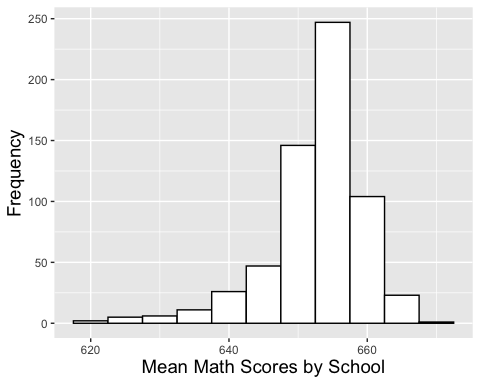
\includegraphics[width=0.6\linewidth]{bookdown-bysh_files/figure-latex/lon-hist1-1} 

}

\caption{Histogram of mean sixth grade MCA math test scores over the years 2008-2010 for 618 Minnesota schools.}\label{fig:lon-hist1}
\end{figure}

\begin{figure}

{\centering 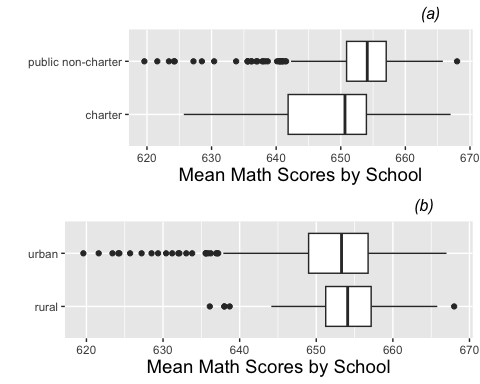
\includegraphics[width=0.6\linewidth]{bookdown-bysh_files/figure-latex/lon-box1-1} 

}

\caption{Boxplots of categorical Level Two covariates vs. average MCA math scores.  Plot (a) shows charter vs. public non-charter schools, while plot (b) shows urban vs. rural schools.}\label{fig:lon-box1}
\end{figure}

\begin{figure}

{\centering 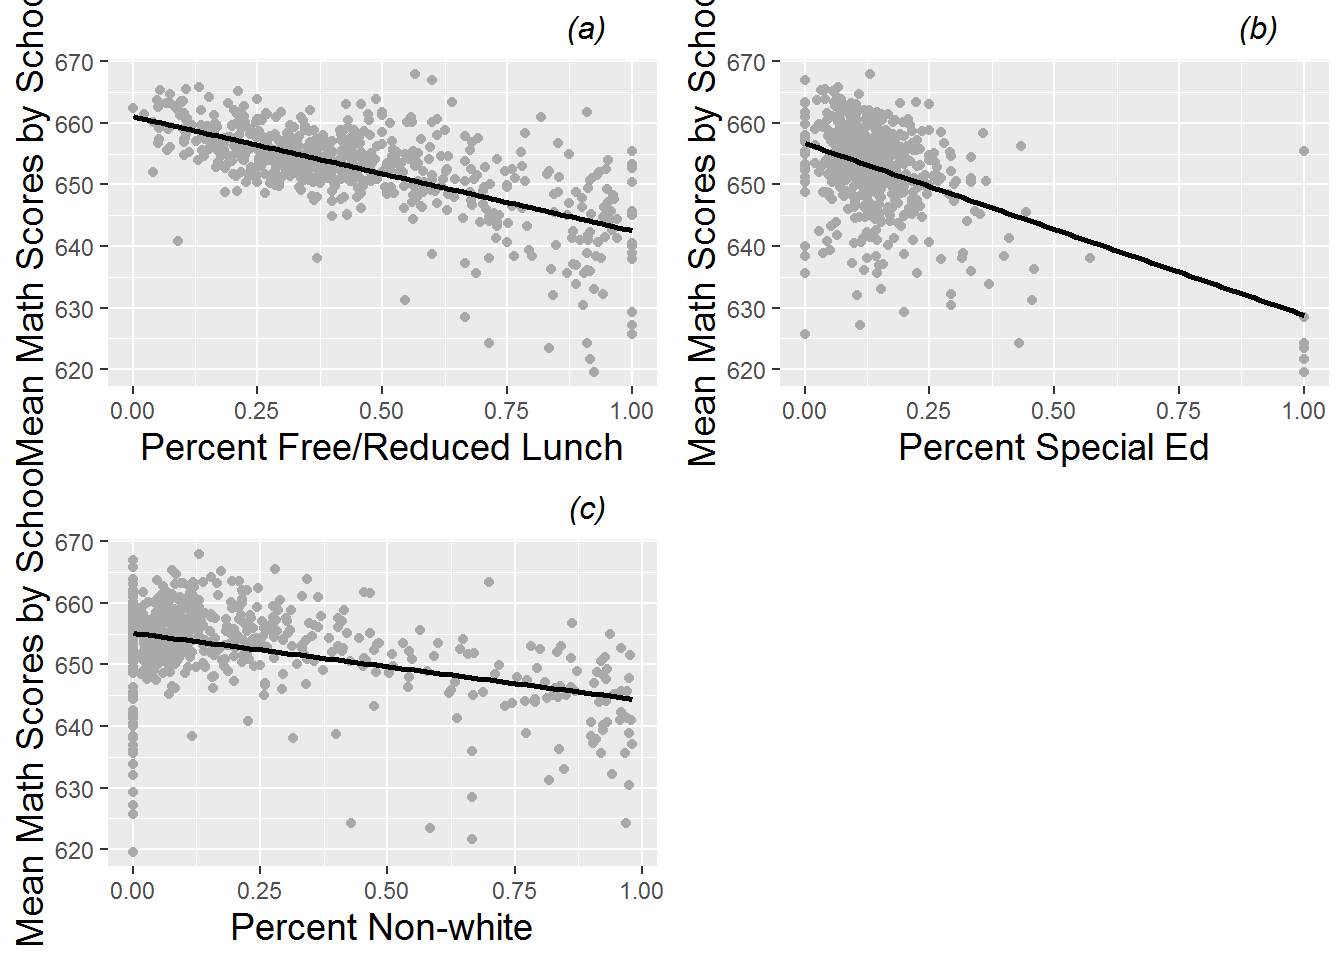
\includegraphics[width=0.6\linewidth]{bookdown-bysh_files/figure-latex/lon-scat1-1} 

}

\caption{ Scatterplots of average MCA math scores by (a) percent free and reduced lunch, (b) percent special education, and (c) percent non-white in a school.}\label{fig:lon-scat1}
\end{figure}

\hypertarget{longitudinalanalyses}{%
\subsection{Exploratory analyses for longitudinal data}\label{longitudinalanalyses}}

In addition to the initial exploratory analyses above, longitudinal data---multilevel data with time at Level One---calls for further plots and summaries that describe time trends within and across individuals. For example, we can examine trends over time within individual schools. Figure \ref{fig:lon-lat1} provides a \textbf{lattice plot} \index{lattice plot} illustrating trends over time for the first 24 schools in the data set. We note differences among schools in starting point (test scores in 2008), slope (change in test scores over the three year period), and form of the relationship. These differences among schools are nicely illustrated in so-called \textbf{spaghetti plots} \index{spaghetti plot} such as Figure \ref{fig:lon-spag1}, which overlays the individual schools' time trends (for the math test scores) from Figure \ref{fig:lon-lat1} on a single set of axes. In order to illustrate the overall time trend without making global assumptions about the form of the relationship, we overlaid in bold a nonparametric fitted curve through a \textbf{loess smoother} \index{loess smoother}. LOESS comes from ``locally weighted scatterplot smoother'', in which a low-degree polynomial is fit to each data point using weighted regression techniques, where nearby points receive greater weight. LOESS is a computationally intensive method which performs especially well with larger sets of data, although ideally there would be a greater diversity of x-values than the three time points we have. In this case, the loess smoother follows very closely to a linear trend, indicating that assuming a linear increase in test scores over the three year period is probably a reasonable simplifying assumption. To further examine the hypothesis that linearity would provide a reasonable approximation to the form of the individual time trends in most cases, Figure \ref{fig:lon-lat2} shows a lattice plot containing linear fits through ordinary least squares rather than connected time points as in Figure \ref{fig:lon-lat1}.

\begin{figure}

{\centering 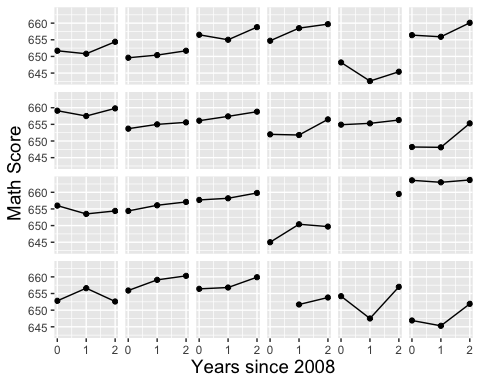
\includegraphics[width=0.6\linewidth]{bookdown-bysh_files/figure-latex/lon-lat1-1} 

}

\caption{Lattice plot by school of math scores over time for the first 24 schools in the data set.}\label{fig:lon-lat1}
\end{figure}

\begin{figure}

{\centering 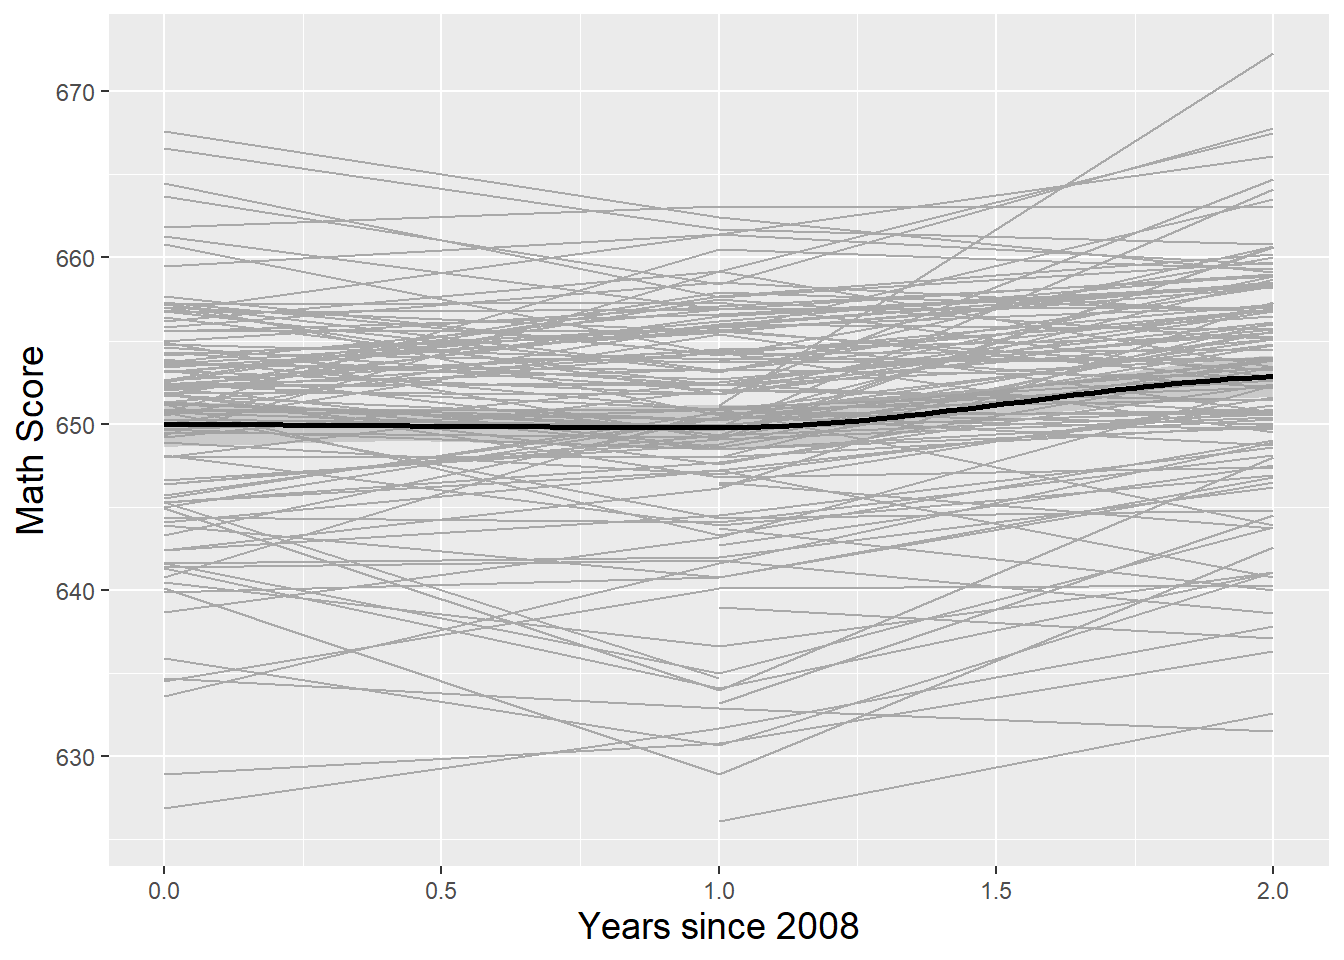
\includegraphics[width=0.6\linewidth]{bookdown-bysh_files/figure-latex/lon-spag1-1} 

}

\caption{ Spaghetti plot of math scores over time by school, for all the charter schools and a random sample of public non-charter schools, with overall fit using loess (bold).}\label{fig:lon-spag1}
\end{figure}

\begin{figure}

{\centering 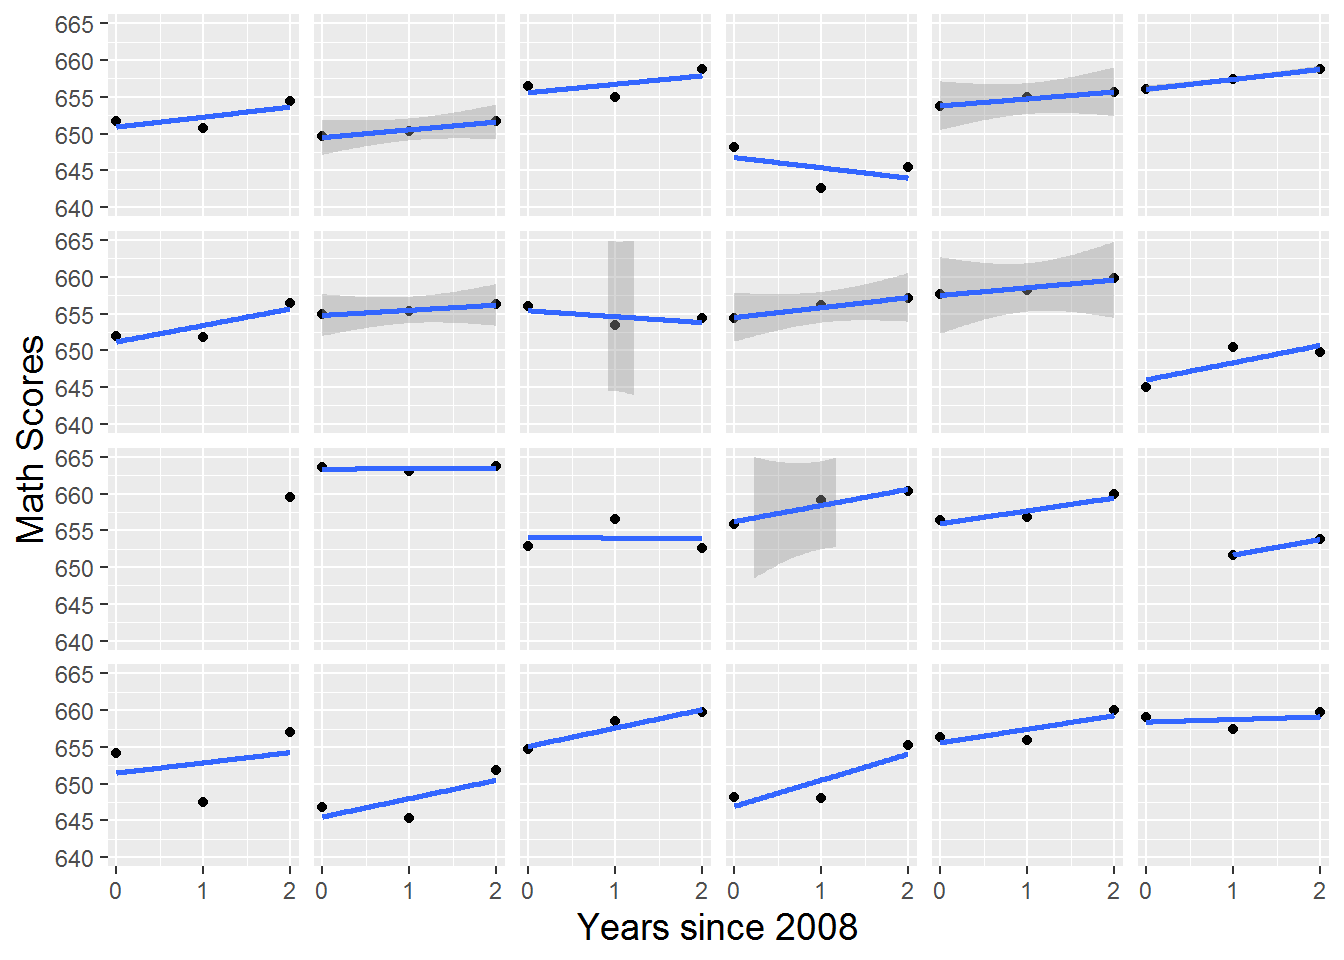
\includegraphics[width=0.6\linewidth]{bookdown-bysh_files/figure-latex/lon-lat2-1} 

}

\caption{ Lattice plot by school of math scores over time with linear fit for the first 24 schools in the data set.}\label{fig:lon-lat2}
\end{figure}

\begin{figure}

{\centering 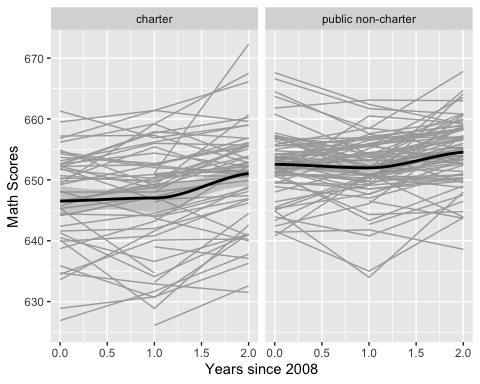
\includegraphics[width=0.6\linewidth]{bookdown-bysh_files/figure-latex/lon-spag3-1} 

}

\caption{Spaghetti plots showing time trends for each school by school type, for a random sample of charter schools (left) and public non-charter schools (right), with overall fits using loess (bold).}\label{fig:lon-spag3}
\end{figure}

\begin{figure}

{\centering 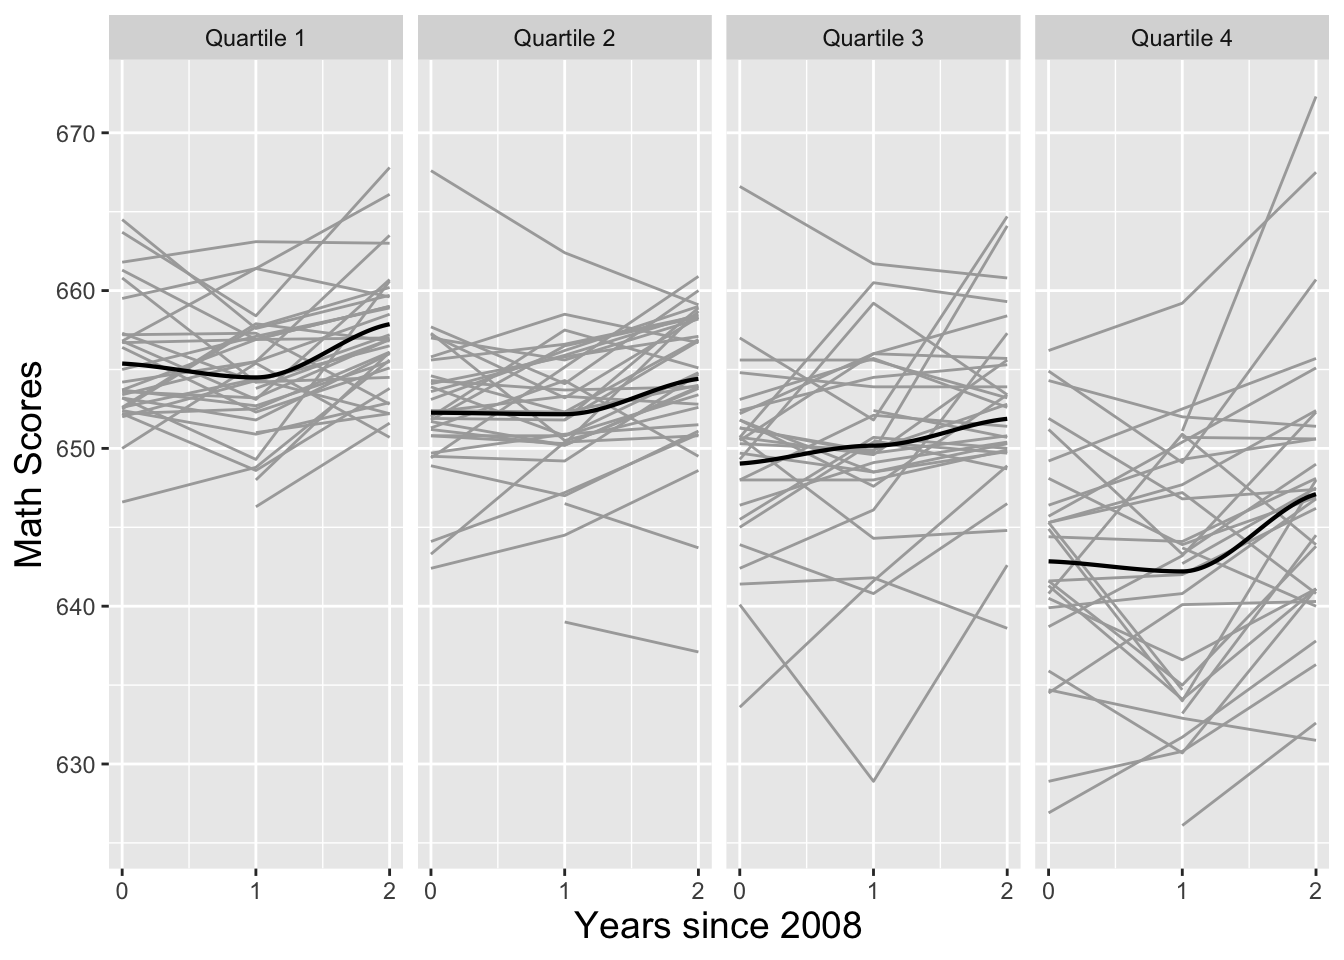
\includegraphics[width=0.6\linewidth]{bookdown-bysh_files/figure-latex/lon-spagmat1-1} 

}

\caption{Spaghetti plots showing time trends for each school by quartiles of percent free and reduced lunch, with loess fits.}\label{fig:lon-spagmat1}
\end{figure}

Just as we explored the relationship between our response (average math scores) and important covariates in Section \ref{generalanalyses}, we can now examine the relationships between time trends by school and important covariates. For instance, Figure \ref{fig:lon-spag3} shows that charter schools had math scores that were lower on average than public non-charter schools and more variable. This type of plot is sometimes called a \textbf{trellis graph} \index{trellis graph}, since it displays a grid of smaller charts with consistent scales, where each smaller chart represents a condition---an item in a category. Trends over time by school type are denoted by bold loess curves. Public non-charter schools have higher scores across all years; both school types show little growth between 2008 and 2009, but greater growth between 2009 and 2010, especially charter schools. Exploratory analyses like this can be repeated for other covariates, such as percent free and reduced lunch in Figure \ref{fig:lon-spagmat1}. The trellis plot automatically divides schools into four groups based on quartiles of their percent free and reduced lunch, and we see that schools with lower percentages of free and reduced lunch students tend to have higher math scores and less variability. Across all levels of free and reduced lunch, we see greater gains between 2009 and 2010 than between 2008 and 2009.

\hypertarget{twostage9}{%
\section{Preliminary two-stage modeling}\label{twostage9}}

\hypertarget{lineartwostage}{%
\subsection{Linear trends within schools}\label{lineartwostage}}

Even though we know that every school's math test scores were not strictly linearly increasing or decreasing over the observation period, a linear model for individual time trends is often a simple but reasonable way to model data. One advantage of using a linear model within school is that each school's data points can be summarized with two summary statistics---an intercept and a slope (obviously, this is an even bigger advantage when there are more observations over time per school). For instance, we see in Figure \ref{fig:lon-lat2} that sixth graders from the school depicted in the top right slot slowly increased math scores over the three year observation period, while students from the school depicted in the fourth column of the top row generally experienced decreasing math scores over the same period. As a whole, the linear model fits individual trends pretty well, and many schools appear to have slowly increasing math scores over time, as researchers in this study may have hypothesized.

Another advantage of assuming a linear trend at Level One (within schools) is that we can examine summary statistics across schools. Both the intercept and slope are meaningful for each school: the \emph{intercept} conveys the school's math score in 2008, while the \emph{slope} conveys the school's average yearly increase or decrease in math scores over the three year period. Figure \ref{fig:lon-cis1} shows that point estimates and uncertainty surrounding individual estimates of intercepts and slopes vary considerably. In addition, we can generate summary statistics and histograms for the 618 intercepts and slopes produced by fitting linear regression models at Level One, in addition to R-square values which describe the strength of fit of the linear model for each school (Figure \ref{fig:lon-histmat1}). For our 618 schools, the mean math score for 2008 was 651.4 (SD=7.28), and the mean yearly rate of change in math scores over the three year period was 1.30 (SD=2.51). We can further examine the relationship between schools' intercepts and slopes. Figure \ref{fig:lon-scat5} shows a general decreasing trend, suggesting that schools with lower 2008 test scores tend to have greater growth in scores between 2008 and 2010 (potentially because those schools have more room for improvement); this trend is supported with a correlation coefficient of -0.32 between fitted intercepts and slopes. Note that, with only 3 or fewer observations for each school, extreme or intractable values for the slope and R-square are possible. For example, slopes cannot be estimated for those schools with just a single test score, R-square values cannot be calculated for those schools with no variability in test scores between 2008 and 2010, and R-square values must be 1 for those schools with only two test scores.



\begin{figure}

{\centering 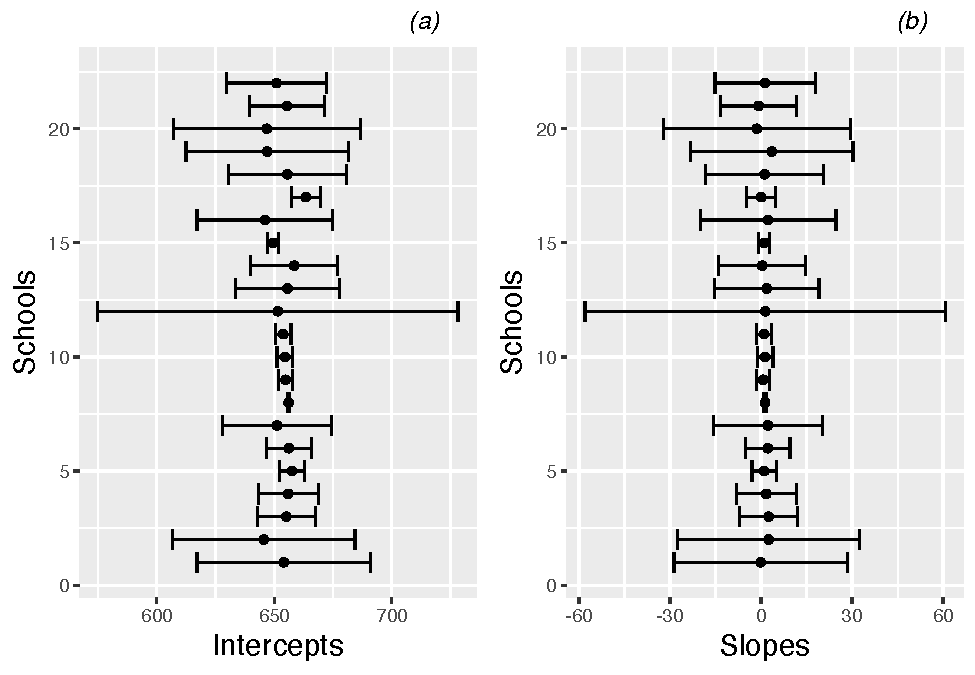
\includegraphics[width=0.6\linewidth]{bookdown-bysh_files/figure-latex/lon-cis1-1} 

}

\caption{Point estimates and 95\% confidence intervals for (a) intercepts and (b) slopes by school, for the first 24 schools in the data set.}\label{fig:lon-cis1}
\end{figure}

\begin{figure}

{\centering 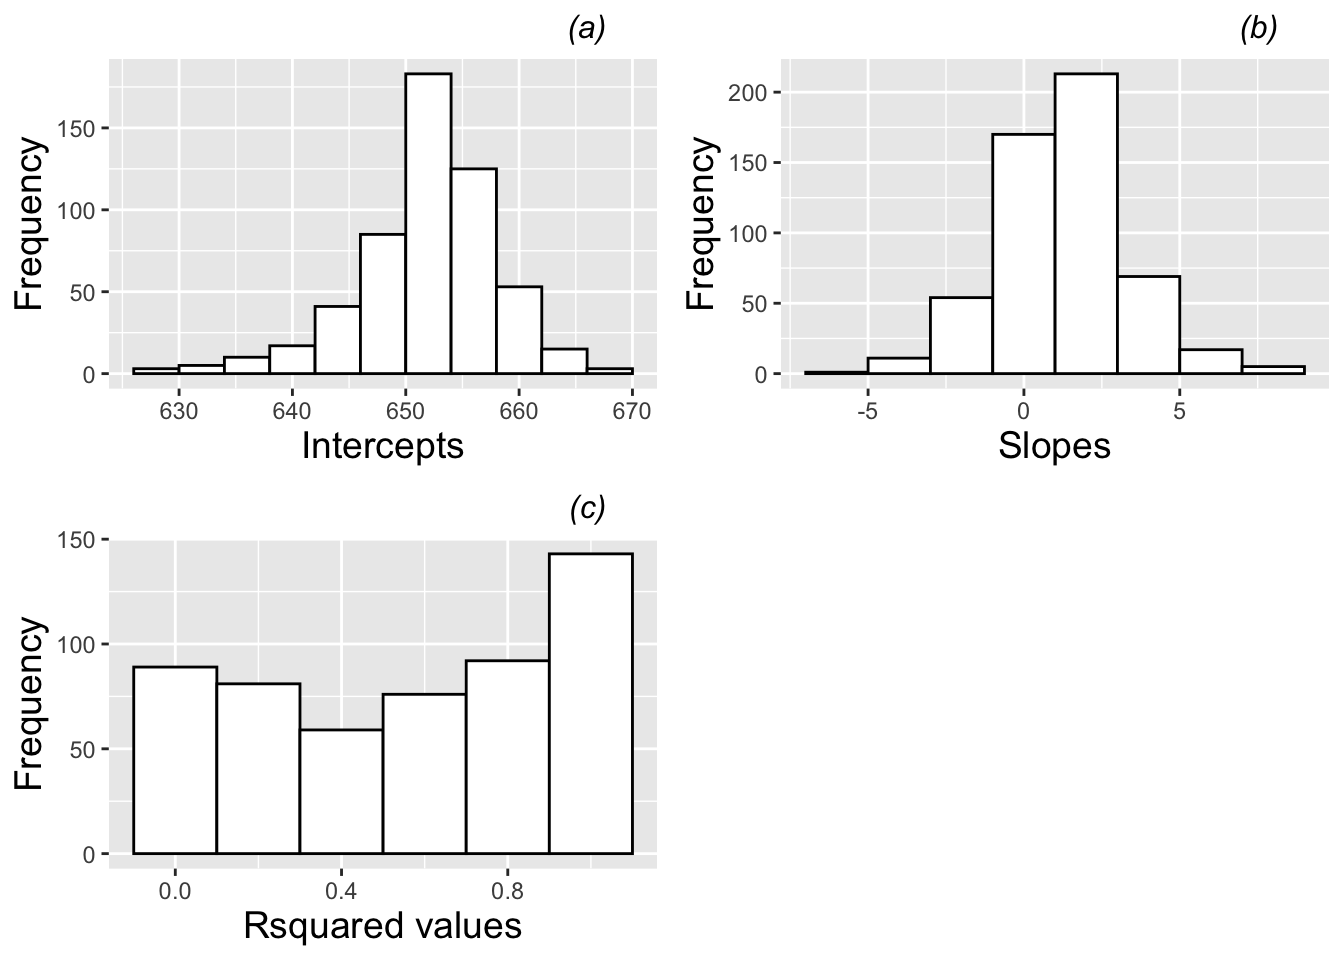
\includegraphics[width=0.6\linewidth]{bookdown-bysh_files/figure-latex/lon-histmat1-1} 

}

\caption{ Histograms for (a) intercepts, (b) slopes, and (c) R-square values from fitted regression lines by school.}\label{fig:lon-histmat1}
\end{figure}

\begin{figure}

{\centering 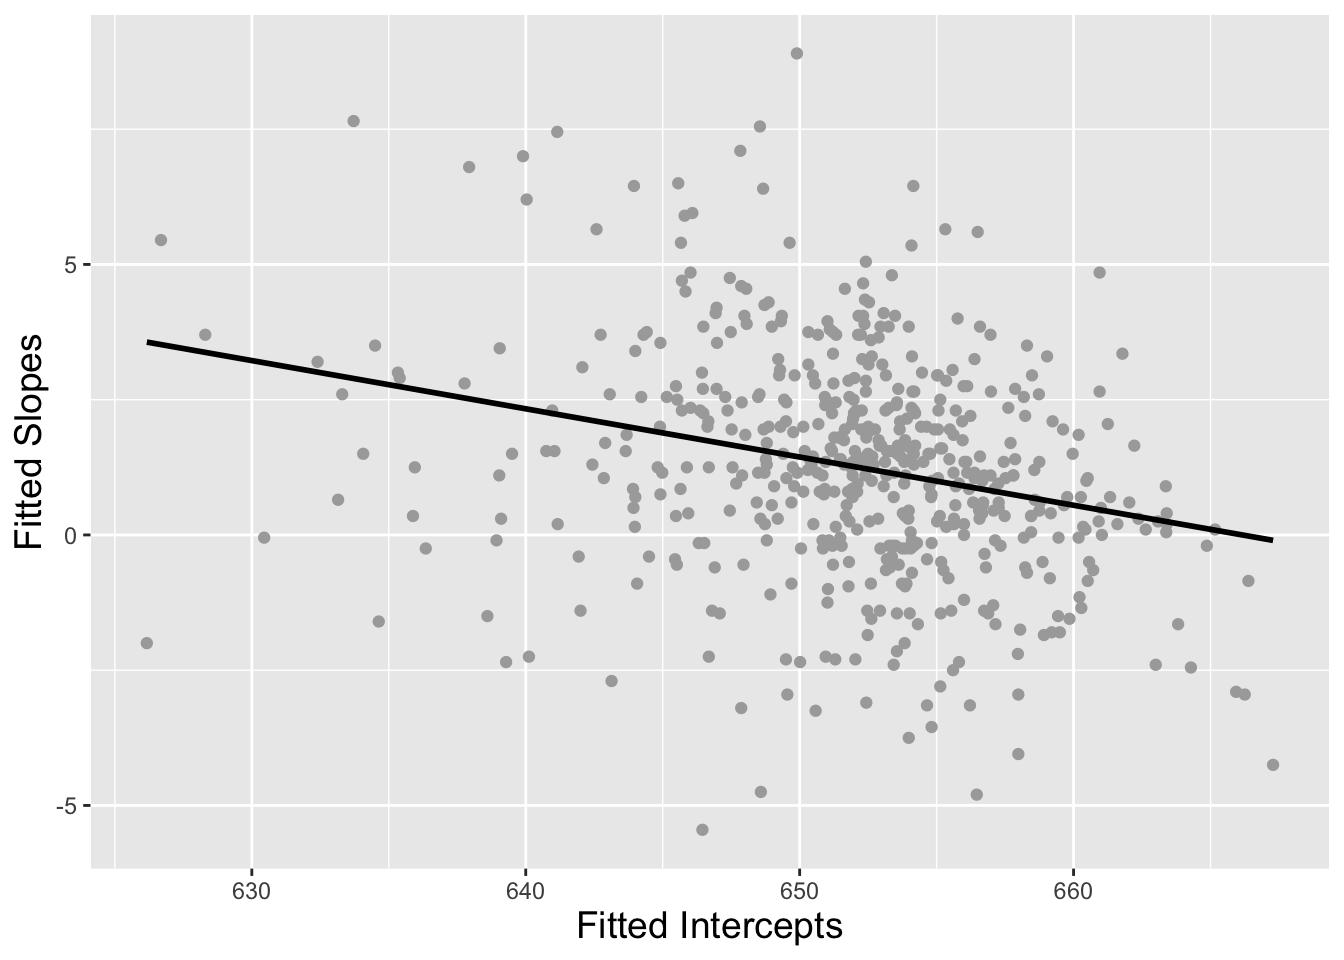
\includegraphics[width=0.6\linewidth]{bookdown-bysh_files/figure-latex/lon-scat5-1} 

}

\caption{Scatterplot showing the relationship between intercepts and slopes from fitted regression lines by school.}\label{fig:lon-scat5}
\end{figure}

\hypertarget{lineartwostageL2effects}{%
\subsection{Effects of level two covariates on linear time trends}\label{lineartwostageL2effects}}

Summarizing trends over time within schools is typically only a start, however. Most of the primary research questions from this study involve comparisons among schools, such as: (a) are there significant differences between charter schools and public non-charter schools, and (b) do any differences between charter schools and public schools change with percent free and reduced lunch, percent special education, or location? These are Level Two questions, and we can begin to explore these questions by graphically examining the effects of school-level variables on schools' linear time trends. By school-level variables, we are referring to those covariates that differ by school but are not dependent on time. For example school type (charter or public non-charter), urban or rural location, percent non-white, percent special education, and percent free and reduced lunch are all variables which differ by school but which don't change over time, at least as they were assessed in this study. Variables which would be time-dependent include quantities such as per pupil funding and reading scores.

Figure \ref{fig:lon-box2} shows differences in the average time trends by school type, using estimated intercepts and slopes to support observations from the spaghetti plots in Figure \ref{fig:lon-spag3}. Based on intercepts, charter schools have lower math scores, on average, in 2008 than public non-charter schools. Based on slopes, however, charter schools tend to improve their math scores at a slightly faster rate than public schools, especially at the seventy-fifth percentile and above. By the end of the three year observation period we would nevertheless expect charter schools to have lower average math scores than public schools. For another exploratory perspective on school type comparisons, we can examine differences between school types with respect to math scores in 2008 and math scores in 2010. As expected, boxplots by school type (Figure \ref{fig:lon-box3}) show clearly lower math scores for charter schools in 2008, but differences are slightly less dramatic in 2010.

\begin{figure}

{\centering 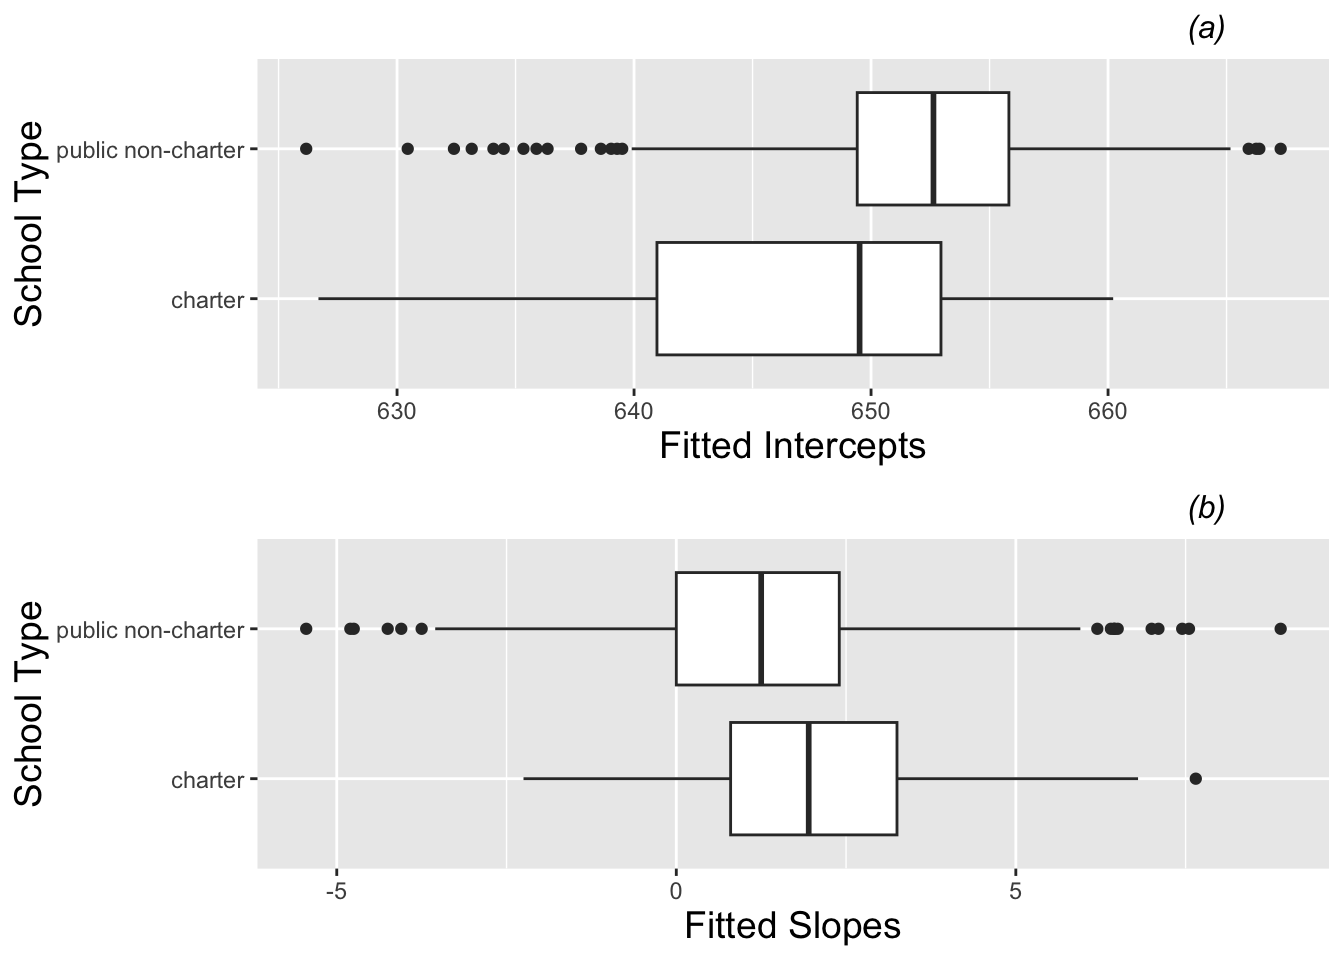
\includegraphics[width=0.6\linewidth]{bookdown-bysh_files/figure-latex/lon-box2-1} 

}

\caption{Boxplots of (a) intercepts and (b) slopes by school type (charter vs. public non-charter).}\label{fig:lon-box2}
\end{figure}

\begin{figure}

{\centering 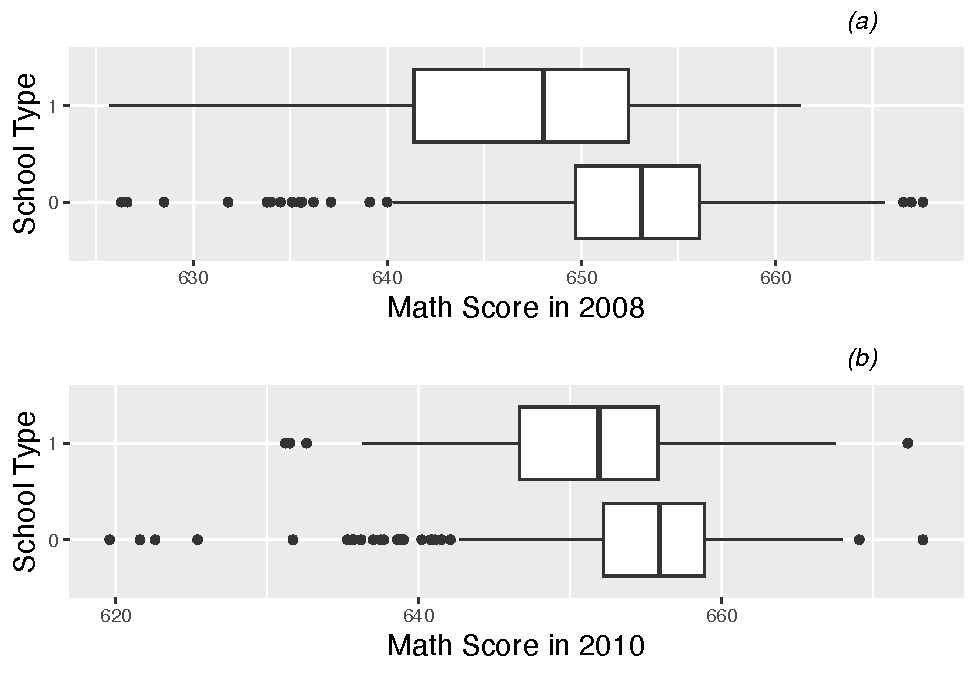
\includegraphics[width=0.6\linewidth]{bookdown-bysh_files/figure-latex/lon-box3-1} 

}

\caption{Boxplots of (a) 2008 and (b) 2010 math scores by school type (charter vs. public non-charter).}\label{fig:lon-box3}
\end{figure}

Any initial exploratory analyses should also investigate effects of potential confounding variables such as school demographics and location. If we discover, for instance, that those schools with higher levels of poverty (measured by the percentage of students receiving free and reduced lunch) display lower test scores in 2008 but greater improvements between 2008 and 2010, then we might be able to use percentage of free and reduced lunch in statistical modeling of intercepts and slopes, leading to more precise estimates of the charter school effects on these two outcomes. In addition, we should also look for any interaction with school type---any evidence that the difference between charter and non-charter schools changes based on the level of a confounding variable. For example, do charter schools perform better relative to non-charter schools when there is a large percentage of non-white students at a school?

With a confounding variable such as percentage of free and reduced lunch, we will treat this variable as continuous to produce the most powerful exploratory analyses. We can begin by examining boxplots of free and reduced lunch percentage against school type (Figure \ref{fig:lon-boxcatmat1}). We observe that charter schools tend to have greater percentages of free and reduced lunch students as well as greater school-to-school variability. Next, we can use scatterplots to graphically illustrate the relationships between free and reduced lunch percentages and significant outcomes such as intercept and slope (also Figure \ref{fig:lon-boxcatmat1}). In this study, it appears that schools with higher levels of free and reduced lunch (i.e., greater poverty) tend to have lower math scores in 2008, but there is little evidence of a relationship between levels of free and reduced lunch and improvements in test scores between 2008 and 2010. These observations are supported with correlation coefficients between percent free and reduced lunch and intercepts (r=-0.61) and slopes (r=-0.06).

A less powerful but occasionally informative way to look at the effect of a continuous confounder on an outcome variables is by creating a categorical variable out of the confounder. For instance, we could classify any school with a percentage of free and reduced lunch students above the median as having a high percentage of free and reduced lunch students and all other schools as having a low percentage of free and reduced lunch students. Then we could examine a possible interaction between percent free and reduced lunch and school type through a series of four boxplots (Figure \ref{fig:lon-boxmat1}). In fact, these boxplots suggest that the gap between charter and public non-charter schools in 2008 was greater in schools with a high percentage of free and reduced lunch students, while the difference in rate of change in test scores between charter and public non-charter schools appeared similar for high and low levels of free and reduced lunch. We will investigate these trends more thoroughly with statistical modeling.

\begin{figure}

{\centering 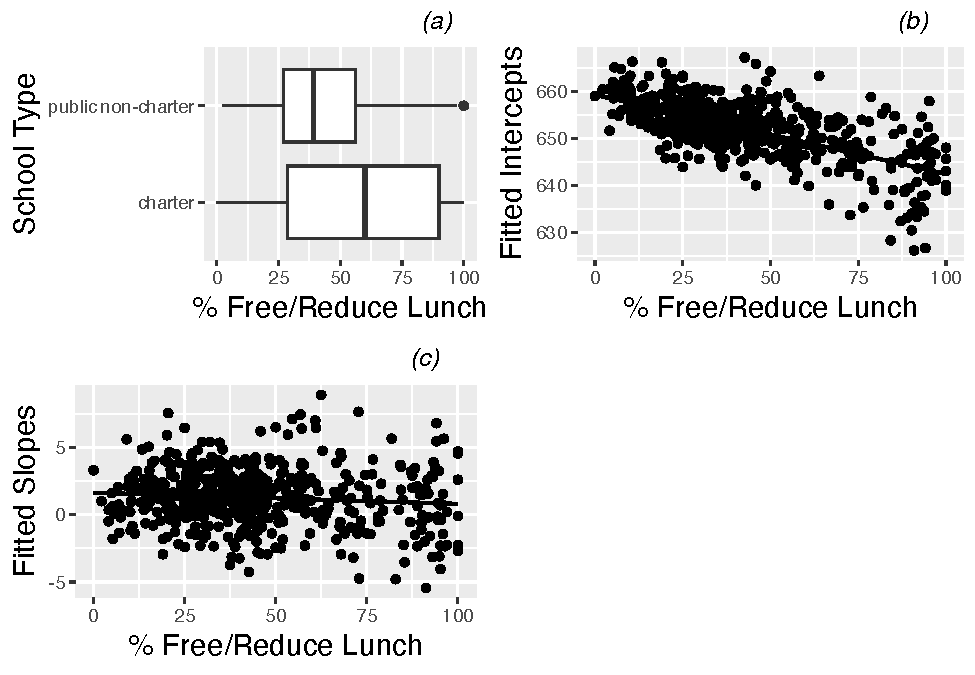
\includegraphics[width=0.6\linewidth]{bookdown-bysh_files/figure-latex/lon-boxcatmat1-1} 

}

\caption{(a) Boxplot of percent free and reduced lunch by school type (charter vs. public non-charter), along with scatterplots of (b) intercepts and (c) slopes from fitted regression lines by school vs. percent free and reduced lunch.}\label{fig:lon-boxcatmat1}
\end{figure}

\begin{figure}

{\centering 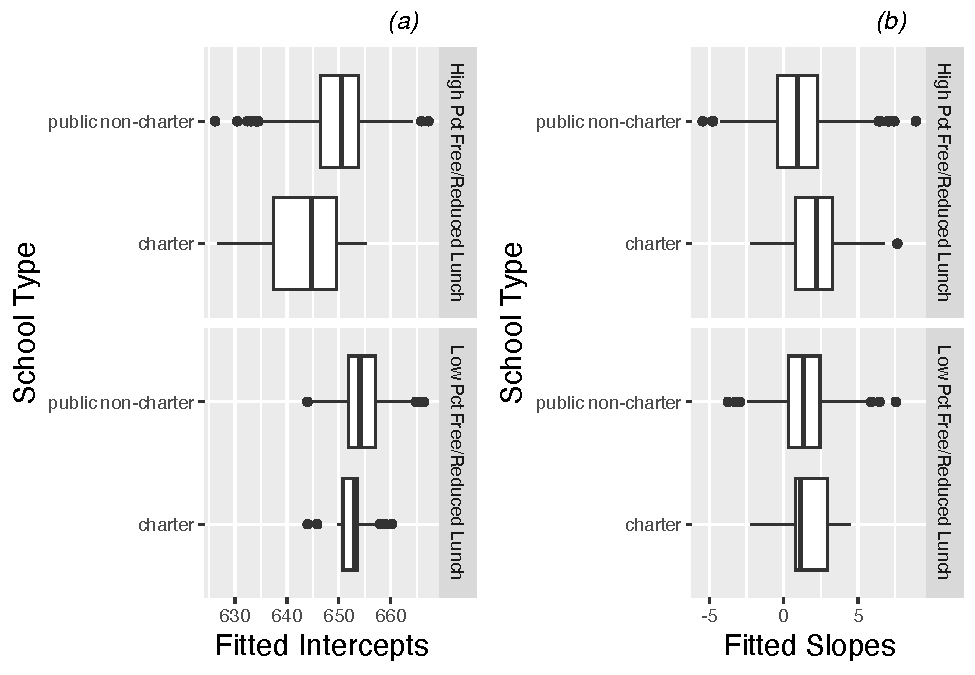
\includegraphics[width=0.6\linewidth]{bookdown-bysh_files/figure-latex/lon-boxmat1-1} 

}

\caption{Boxplots of (a) intercepts and (b) slopes from fitted regression lines by school vs. school type (charter vs. public non-charter), separated by high and low levels of percent free and reduced lunch.}\label{fig:lon-boxmat1}
\end{figure}

The effect of other confounding variables (e.g., percent non-white, percent special education, urban or rural location) can be investigated in a similar fashion to free and reduced lunch percentage, both in terms of main effect (variability in outcomes such as slope and intercept which can be explained by the confounding variable) and interaction with school type (ability of the confounding variable to explain differences between charter and public non-charter schools). We leave these explorations as an exercise.

\hypertarget{lineartwostageerror2}{%
\subsection{Error structure within schools}\label{lineartwostageerror2}}

Finally, with longitudinal data it is important to investigate the error variance-covariance structure of data collected within a school (the Level Two observational unit). In multilevel data, as in the examples we introduced in Chapter \ref{ch-corrdata}, we suspect observations within group (like a school) to be correlated, and we strive to model that correlation. When the data within group is collected over time, we often see distinct patterns in the residuals that can be modeled---correlations which decrease systematically as the time interval increases, variances that change over time, correlation structure that depends on a covariate, etc. A first step in modeling the error variance-covariance structure is the production of an exploratory plot such as Figure \ref{fig:lon-cor1}. To generate this plot, we begin by modeling MCA math score as a linear function of time using all 1733 observations and ignoring the school variable. This population (marginal) trend is illustrated in Figure \ref{fig:lon-spag1} and is given by:

\begin{equation*}
\hat{Y}_{ij}=651.69+1.20\textrm{Time}_{ij},
\end{equation*}
where \(\hat{Y}_{ij}\) is the predicted math score of the \(i^{th}\) school at time \(j\), where time \(j\) is the number of years since 2008. In this model, the predicted math score will be identical for all schools at a given time point \(j\). Residuals \(Y_{ij}-\hat{Y}_{ij}\) are then calculated for each observation, measuring the difference between actual math score and the average overall time trend. Figure \ref{fig:lon-cor1} then combines three pieces of information: the upper right triangle contains correlation coefficients for residuals between pairs of years, the diagonal contains histograms of residuals at each time point, and the lower left triangle contains scatterplots of residuals from two different years. In our case, we see that correlation between residuals from adjacent years is strongly positive (0.81-0.83) and does not drop off greatly as the time interval between years increases.

\begin{figure}

{\centering 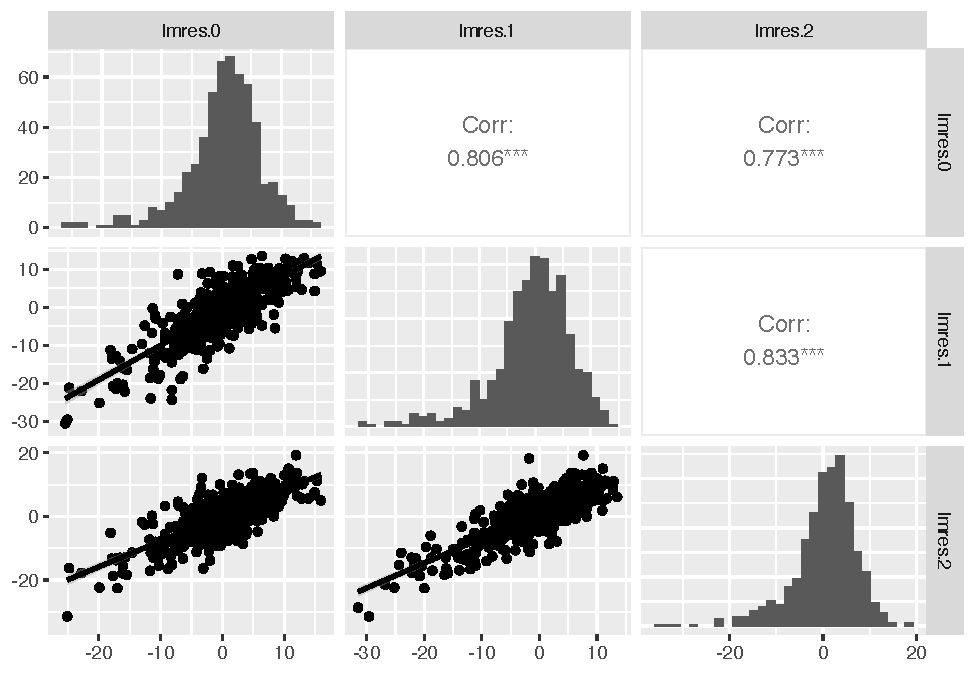
\includegraphics[width=0.6\linewidth]{bookdown-bysh_files/figure-latex/lon-cor1-1} 

}

\caption{Correlation structure within school.  The upper right contains correlation coefficients between residuals at pairs of time points, the lower left contains scatterplots of the residuals at time point pairs, and the diagonal contains histograms of residuals at each of the three time points.}\label{fig:lon-cor1}
\end{figure}

\hypertarget{lineartwostageerror}{%
\section{Initial models}\label{lineartwostageerror}}

Throughout the exploratory analysis phase, our original research questions have guided our work, and now with modeling we return to familiar questions such as:

\begin{itemize}
\tightlist
\item
  are differences between charter and public non-charter schools (in intercept, in slope, in 2010 math score) statistically significant?
\item
  are differences between school types statistically significant, even after accounting for school demographics and location?
\item
  do charter schools offer any measurable benefit over non-charter public schools, either overall or within certain subgroups of schools based on demographics or location?
\end{itemize}

As you might expect, answers to these questions will arise from proper consideration of variability and properly identified statistical models.
As in Chapter \ref{ch-multilevelintro}, we will begin model fitting with some simple, preliminary models, in part to establish a baseline for evaluating larger models. Then, we can build toward a final model for inference by attempting to add important covariates, centering certain variables, and checking assumptions.

\hypertarget{modela}{%
\subsection{Unconditional means model}\label{modela}}

In the multilevel context, we almost always begin with the \textbf{unconditional means model} \index{unconditional means model}, in which there are no predictors at any level. The purpose of the unconditional means model is to assess the amount of variation at each level, and to compare variability within school to variability between schools. Define \(Y_{ij}\) as the MCA-II math score from school \(i\) and year \(j\). Using the composite model specification from Chapter \ref{ch-multilevelintro}:

\begin{equation*}
Y _{ij} = \alpha_{0} + u_{i} + \epsilon_{ij} \textrm{ with } u_{i} \sim N(0, \sigma^2_u) \textrm{ and } \epsilon_{ij} \sim N(0, \sigma^2)
\end{equation*}
the unconditional means model can be fit to the MCA-II data:

\begin{Shaded}
\begin{Highlighting}[]
\CommentTok{#Model A (Unconditional means model)}
\NormalTok{model.a <-}\StringTok{ }\KeywordTok{lmer}\NormalTok{(MathAvgScore}\OperatorTok{~}\StringTok{ }\DecValTok{1} \OperatorTok{+}\StringTok{ }\NormalTok{(}\DecValTok{1}\OperatorTok{|}\NormalTok{schoolid), }
                \DataTypeTok{REML=}\NormalTok{T, }\DataTypeTok{data=}\NormalTok{chart.long)}
\end{Highlighting}
\end{Shaded}

\begin{verbatim}
##  Groups   Name        Variance Std.Dev.
##  schoolid (Intercept) 41.9     6.47    
##  Residual             10.6     3.25
\end{verbatim}

\begin{verbatim}
##  Number of Level Two groups =  618
\end{verbatim}

\begin{verbatim}
##             Estimate Std. Error t value
## (Intercept)    652.7     0.2726    2395
\end{verbatim}

From this output, we obtain estimates of our three model parameters:

\begin{itemize}
\item
  \(\hat{\alpha}_{0}\) = 652.7 = the mean math score across all schools and all years
\item
  \(\hat{\sigma}^2\)= 10.6 = the variance in within-school deviations between individual scores and the school mean across all years
\item
  \(\hat{\sigma}^2_u\)= 41.9 = the variance in between-school deviations between school means and the overall mean across all schools and all years
\end{itemize}

Based on the intraclass correlation coefficient:

\begin{equation*}
\hat{\rho}=\frac{\hat{\sigma}^2_u}{\hat{\sigma}^2_u + \hat{\sigma}^2} = \frac{41.869}{41.869+10.571}= 0.798
\end{equation*}
79.8 percent of the total variation in math scores is attributable to difference among schools rather than changes over time within schools. We can also say that the average correlation for any pair of responses from the same school is 0.798.

\hypertarget{modelb9}{%
\subsection{Unconditional growth model}\label{modelb9}}

The second model in most multilevel contexts introduces a covariate at Level One (see Model B in Chapter \ref{ch-multilevelintro}). With longitudinal data, this second model introduces time as a predictor at Level One, but there are still no predictors at Level Two. This model is then called the \textbf{unconditional growth model} \index{unconditional growth model}. The unconditional growth model allows us to assess how much of the within-school variability can be attributed to systematic changes over time.

At the lowest level, we can consider building individual growth models over time for each of the 618 schools in our study. First, we must decide upon a form for each of our 618 growth curves. Based on our initial exploratory analyses, assuming that an individual school's MCA-II math scores follow a linear trend seems like a reasonable starting point. Under the assumption of linearity, we must estimate an intercept and a slope for each school, based on their 1-3 test scores over a period of three years. Compared to time series analyses of economic data, most longitudinal data analyses have relatively few time periods for each subject (or school), and the basic patterns within subject are often reasonably described by simpler functional forms.

Let \(Y_{ij}\) be the math score of the \(i^{th}\) school in year \(j\). Then we can model the linear change in math test scores over time for School \(i\) according to Model B:

\begin{equation*}
Y_{ij} = a_{i} + b_{i}\textrm{Year08}_{ij} + \epsilon_{ij} \textrm{ where } \epsilon_{ij} \sim N(0, \sigma^2)
\end{equation*}

The parameters in this model \((a_{i}, b_{i},\) and \(\sigma^2)\) can be estimated through LLSR methods. \(a_{i}\) represents the true intercept for School \(i\)---i.e., the expected test score level for School \(i\) when time is zero (2008)---while \(b_{i}\) represents the true slope for School \(i\)---i.e., the expected yearly rate of change in math score for School \(i\) over the three year observation period. Here we use Roman letters rather than Greek for model parameters since models by school will eventually be a conceptual first step in a multilevel model. The \(\epsilon_{ij}\) terms represent the deviation of School \(i\)'s actual test scores from the expected results under linear growth---the part of school \(i\)'s test score at time \(j\) that is not explained by linear changes over time. The variability in these deviations from the linear model is given by \(\sigma^2\). In Figure \ref{fig:lon-scat3}, which illustrates a linear growth model for Norwood Central Middle School, \(a_{i}\) is estimated by the \(y\)-intercept of the fitted regression line, \(b_{i}\) is estimated by the slope of the fitted regression line, and \(\sigma^2\) is estimated by the variability in the vertical distances between each point (the actual math score in year \(j\)) and the line (the predicted math score in year \(j\)).

\begin{figure}

{\centering 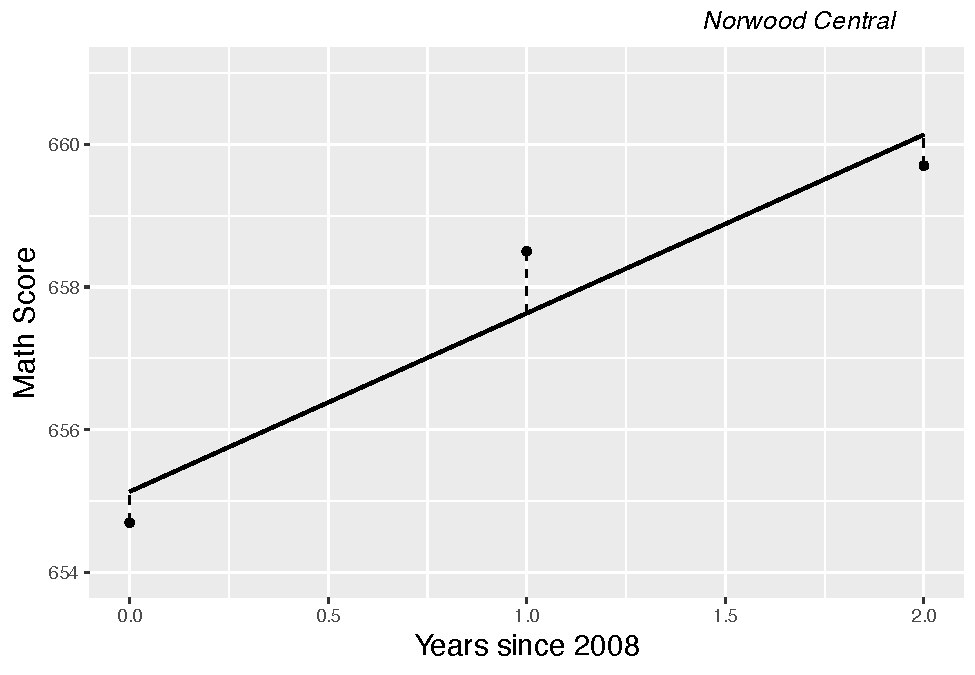
\includegraphics[width=0.6\linewidth]{bookdown-bysh_files/figure-latex/lon-scat3-1} 

}

\caption{Linear growth model for Norwood Central Middle School}\label{fig:lon-scat3}
\end{figure}

In a multilevel model, we let intercepts (\(a_{i}\)) and slopes (\(b_{i}\)) vary by school and build models for these intercepts and slopes using school-level variables at Level Two. An unconditional growth model features no predictors at Level Two and can be specified either using formulations at both levels:

\begin{itemize}
\item
  Level One:
  \begin{equation*}
  Y_{ij}=a_{i}+b_{i}\textrm{Year08}_{ij} + \epsilon_{ij}
  \end{equation*}
\item
  Level Two:
  \begin{align*}
  a_{i}&=\alpha_{0} + u_{i}\\
  b_{i}&=\beta_{0} + v_{i}
  \end{align*}
\end{itemize}

or as a composite model:

\begin{equation*}
Y_{ij}=\alpha_{0} + \beta_{0}\textrm{Year08}_{ij}+u_{i}+v_{i}\textrm{Year08}_{ij} + \epsilon_{ij}
\end{equation*}
where \(\epsilon_{ij}\sim N(0,\sigma^2)\) and

\[ \left[ \begin{array}{c}
            u_{i} \\ v_{i}
          \end{array}  \right] \sim N \left( \left[
          \begin{array}{c}
            0 \\ 0
          \end{array} \right], \left[
          \begin{array}{cc}
            \sigma_{u}^{2} & \\
            \sigma_{uv} & \sigma_{v}^{2}
          \end{array} \right] \right) . \]

As before, \(\sigma^2\) quantifies the within-school variability (the scatter of points around schools' linear growth trajectories), while now the between-school variability is partitioned into variability in initial status \((\sigma^2_u)\) and variability in rates of change \((\sigma^2_v)\).

Using the composite model specification, the unconditional growth model can be fit to the MCA-II test data:

\begin{Shaded}
\begin{Highlighting}[]
\CommentTok{#Model B (Unconditional growth)}
\NormalTok{model.b <-}\StringTok{ }\KeywordTok{lmer}\NormalTok{(MathAvgScore}\OperatorTok{~}\StringTok{ }\NormalTok{year08 }\OperatorTok{+}\StringTok{ }\NormalTok{(year08}\OperatorTok{|}\NormalTok{schoolid), }
  \DataTypeTok{REML=}\NormalTok{T, }\DataTypeTok{data=}\NormalTok{chart.long)}
\end{Highlighting}
\end{Shaded}

\begin{verbatim}
##  Groups   Name        Variance Std.Dev. Corr
##  schoolid (Intercept) 39.441   6.280        
##           year08       0.111   0.332    0.72
##  Residual              8.820   2.970
\end{verbatim}

\begin{verbatim}
##  Number of Level Two groups =  618
\end{verbatim}

\begin{verbatim}
##             Estimate Std. Error t value
## (Intercept)  651.408    0.27934 2331.96
## year08         1.265    0.08997   14.06
\end{verbatim}

\begin{verbatim}
##  AIC =  10352 ;  BIC =  10384
\end{verbatim}

From this output, we obtain estimates of our six model parameters:

\begin{itemize}
\tightlist
\item
  \(\hat{\alpha}_{0}\) = 651.4 = the mean math score for the population of schools in 2008.
\item
  \(\hat{\beta}_{0}\) = 1.26 = the mean yearly change in math test scores for the population during the three year observation period.
\item
  \(\hat{\sigma}^2\) = 8.82 = the variance in within-school deviations.
\item
  \(\hat{\sigma}^2_u\) = 39.4 = the variance between schools in 2008 scores.
\item
  \(\hat{\sigma}^2_v\) = 0.11 = the variance between schools in rates of change in math test scores during the three year observation period.
\item
  \(\hat{\rho}_{uv}\) = 0.72 = the correlation in schools' 2008 math score and their rate of change in scores between 2008 and 2010.
\end{itemize}

We see that schools had a mean math test score of 651.4 in 2008 and their mean test scores tended to increase by 1.26 points per year over the three year observation period, producing a mean test score at the end of three years of 653.9. According to the t-value (14.1), the increase in mean test scores noted during the three year observation period is statistically significant.

The estimated within-school variance \(\hat{\sigma}^2\) decreased by about 17\% from the unconditional means model, implying that 17\% of within-school variability in test scores can be explained by a linear increase over time:

\begin{align*}
\textrm{Pseudo }R^2_{L1} & = \frac{\hat{\sigma}^2(\textrm{uncond means}) - \hat{\sigma}^2(\textrm{uncond growth})}{\hat{\sigma^2}(\textrm{uncond means})} \\
 & = \frac{10.571-8.820}{10.571}= 0.17
\end{align*}

\hypertarget{othertimetrends}{%
\subsection{Modeling other trends over time}\label{othertimetrends}}

While modeling linear trends over time is often a good approximation of reality, it is by no means the only way to model the effect of time. One alternative is to model the quadratic effect of time, which implies adding terms for both time and the square of time. Typically, to reduce the correlation between the linear and quadratic components of the time effect, the time variable is often centered first; we have already ``centered'' on 2008. Modifying Model B to produce an \textbf{unconditional quadratic growth model} would take the following form:

\begin{itemize}
\item
  Level One:
  \begin{equation*}
  Y_{ij}=a_{i}+b_{i}\textrm{Year08}_{ij}+c_{i}\textrm{Year08}^{2}_{ij} + \epsilon_{ij}
  \end{equation*}
\item
  Level Two:
  \begin{align*}
  a_{i} & = \alpha_{0} + u_{i}\\
  b_{i} & = \beta_{0} + v_{i}\\
  c_{i} & = \gamma_{0} + w_{i}
  \end{align*}
  where \(\epsilon_{ij}\sim N(0,\sigma^2)\) and
\end{itemize}

\[ \left[ \begin{array}{c}
            u_{i} \\ v_{i} \\ w_{i}
          \end{array}  \right] \sim N \left( \left[
          \begin{array}{c}
            0 \\ 0 \\ 0
          \end{array} \right], \left[
          \begin{array}{ccc}
            \sigma_{u}^{2} & & \\
            \sigma_{uv} & \sigma_{v}^{2} & \\
            \sigma_{uw} & \sigma_{vw} & \sigma_{w}^{2}
          \end{array} \right] \right) . \]

With the extra term at Level One for the quadratic effect, we now have 3 equations at Level Two, and 6 variance components at Level Two (3 variance terms and 3 covariance terms). However, with only a maximum of 3 observations per school, we lack the data for fitting 3 equations with error terms at Level Two. Instead, we could model the quadratic time effect with fewer variance components---for instance, by only using an error term on the intercept at Level Two:\\
\begin{align*}
a_{i} & = \alpha_{0} + u_{i}\\
b_{i} & = \beta_{0}\\ 
c_{i} & = \gamma_{0}
\end{align*}
where \(u_{i}\sim N(0,\sigma^2_u)\). Models like this are frequently used in practice---they allow for a separate overall effect on test scores for each school while minimizing parameters that must be estimated. The tradeoff is that this model does not allow linear and quadratic effects to differ by school, but we have little choice here without more observations per school. Thus, using the composite model specification, the unconditional quadratic growth model with random intercept for each school can be fit to the MCA-II test data:

\begin{Shaded}
\begin{Highlighting}[]
\CommentTok{# Modeling quadratic time trend}
\NormalTok{model.b2 <-}\StringTok{ }\KeywordTok{lmer}\NormalTok{(MathAvgScore}\OperatorTok{~}\StringTok{ }\NormalTok{yearc }\OperatorTok{+}\StringTok{ }\NormalTok{yearc2 }\OperatorTok{+}\StringTok{ }\NormalTok{(}\DecValTok{1}\OperatorTok{|}\NormalTok{schoolid), }
  \DataTypeTok{REML=}\NormalTok{T, }\DataTypeTok{data=}\NormalTok{chart.long)}
\end{Highlighting}
\end{Shaded}

\begin{verbatim}
##  Groups   Name        Variance Std.Dev.
##  schoolid (Intercept) 43.05    6.56    
##  Residual              8.52    2.92
\end{verbatim}

\begin{verbatim}
##  Number of Level Two groups =  618
\end{verbatim}

\begin{verbatim}
##             Estimate Std. Error  t value
## (Intercept)  651.942    0.29229 2230.448
## yearc          1.270    0.08758   14.501
## yearc2         1.068    0.15046    7.101
\end{verbatim}

\begin{verbatim}
##  AIC =  10308 ;  BIC =  10335
\end{verbatim}

From this output, we see that the quadratic effect is positive and significant (t=7.1), in this case indicating that increases in test scores are greater between 2009 and 2010 than between 2008 and 2009. Based on AIC and BIC values, the quadratic growth model outperforms the linear growth model with random intercepts only at level Two (AIC: 10308 vs.~10354; BIC: 10335 vs.~10375).

Another frequently used approach to modeling time effects is the \textbf{piecewise linear model}. In this model, the complete time span of the study is divided into two or more segments, with a separate slope relating time to the response in each segment. In our case study there is only one piecewise option---fitting separate slopes in 2008-09 and 2009-10. With only 3 time points, creating a piecewise linear model is a bit simplified, but this idea can be generalized to segments with more than two years each.

The performance of this model is very similar to the quadratic growth model by AIC and BIC measures, and the story told by fixed effects estimates is also very similar. While the mean yearly increase in math scores was 0.2 points between 2008 and 2009, it was 2.3 points between 2009 and 2010.

Despite the good performances of the quadratic growth and piecewise linear models on our three-year window of data, we will continue to use linear growth assumptions in the remainder of this chapter. Not only is a linear model easier to interpret and explain, but it's probably a more reasonable assumption in years beyond 2010. Predicting future performance is more risky by assuming a steep one year rise or a non-linear rise will continue, rather than by using the average increase over two years.

\hypertarget{finalmodel}{%
\section{Building to a final model}\label{finalmodel}}

\hypertarget{sec:modelc9}{%
\subsection{Uncontrolled effects of school type}\label{sec:modelc9}}

Initially, we can consider whether or not there are significant differences in individual school growth parameters (intercepts and slopes) based on school type. From a modeling perspective, we would build a system of two Level Two models:

\begin{align*}
a_{i} & = \alpha_{0} + \alpha_{1}\textrm{Charter}_i + u_{i} \\
b_{i} & = \beta_{0} + \beta_{1}\textrm{Charter}_i + v_{i}
\end{align*}
where \(\textrm{Charter}_i=1\) if School \(i\) is a charter school and \(\textrm{Charter}_i=0\) if School \(i\) is a non-charter public school. In addition, the error terms at Level Two are assumed to follow a multivariate normal distribution:

\[ \left[ \begin{array}{c}
            u_{i} \\ v_{i}
          \end{array}  \right] \sim N \left( \left[
          \begin{array}{c}
            0 \\ 0
          \end{array} \right], \left[
          \begin{array}{cc}
            \sigma_{u}^{2} & \\
            \sigma_{uv} & \sigma_{v}^{2}
          \end{array} \right] \right) . \]

With a binary predictor at Level Two such as school type, we can write out what our Level Two model looks like for public non-charter schools and charter schools.

\begin{itemize}
\tightlist
\item
  Public schools
\end{itemize}

\begin{align*}
a_{i} & = \alpha_{0} + u_{i}\\
b_{i} & = \beta_{0} + v_{i},
\end{align*}

\begin{itemize}
\tightlist
\item
  Charter schools
\end{itemize}

\begin{align*}
a_{i} & = (\alpha_{0} + \alpha_{1}) + u_{i}\\
b_{i} & = (\beta_{0}+ \beta_{1}) + v_{i}
\end{align*}

Writing the Level Two model in this manner helps us interpret the model parameters from our two-level model. We can use statistical software (such as the \texttt{lmer()} function from the \texttt{lme4} package in R) to obtain parameter estimates using our \(1733\) observations, after first converting our Level One and Level Two models into a composite model (Model C) with fixed effects and variance components separated:

\begin{align*}
Y_{ij} & = a_{i} + b_{i}\textrm{Year08}_{ij}+ \epsilon_{ij} \\
       & = (\alpha_{0} + \alpha_{1}\textrm{Charter}_i +u_{i}) + (\beta_{0} + \beta_{1}\textrm{Charter}_i + v_{i})\textrm{Year08}_{ij} + \epsilon_{ij} \\
       & = [\alpha_{0} + \beta_{0}\textrm{Year08}_{ij} +\alpha_{1}\textrm{Charter}_i+ \beta_{1}\textrm{Charter}_i\textrm{Year08}_{ij}] + \\
       & \quad [u_{i} + v_{i}\textrm{Year08}_{ij} + \epsilon_{ij}]
\end{align*}

\begin{Shaded}
\begin{Highlighting}[]
\CommentTok{#Model C (uncontrolled effects of school type on }
\CommentTok{#   intercept and slope)}
\NormalTok{model.c <-}\StringTok{ }\KeywordTok{lmer}\NormalTok{(MathAvgScore}\OperatorTok{~}\StringTok{ }\NormalTok{charter }\OperatorTok{+}\StringTok{ }\NormalTok{year08 }\OperatorTok{+}\StringTok{ }
\StringTok{  }\NormalTok{charter}\OperatorTok{:}\NormalTok{year08 }\OperatorTok{+}\StringTok{ }\NormalTok{(year08}\OperatorTok{|}\NormalTok{schoolid), }
  \DataTypeTok{REML=}\NormalTok{T, }\DataTypeTok{data=}\NormalTok{chart.long)}
\end{Highlighting}
\end{Shaded}

\begin{verbatim}
##  Groups   Name        Variance Std.Dev. Corr
##  schoolid (Intercept) 35.832   5.986        
##           year08       0.131   0.362    0.88
##  Residual              8.784   2.964
\end{verbatim}

\begin{verbatim}
##  Number of Level Two groups =  618
\end{verbatim}

\begin{verbatim}
##                Estimate Std. Error  t value
## (Intercept)    652.0584    0.28449 2291.996
## charter         -6.0184    0.86562   -6.953
## year08           1.1971    0.09427   12.698
## charter:year08   0.8557    0.31430    2.723
\end{verbatim}

\begin{verbatim}
##  AIC =  10308 ;  BIC =  10351
\end{verbatim}

Armed with our parameter estimates, we can offer concrete interpretations:

\begin{itemize}
\item
  Fixed effects:

  \begin{itemize}
  \tightlist
  \item
    \(\hat{\alpha}_{0} = 652.1.\) The estimated mean test score for 2008 for non-charter public schools is 652.1.
  \item
    \(\hat{\alpha}_{1}= -6.02.\) Charter schools have an estimated test score in 2008 which is 6.02 points lower than public non-charter schools.
  \item
    \(\hat{\beta}_{0}= 1.20.\) Public non-charter schools have an estimated mean increase in test scores of 1.20 points per year.
  \item
    \(\hat{\beta}_{1}= 0.86.\) Charter schools have an estimated mean increase in test scores of 2.06 points per year over the three year observation period, 0.86 points higher than the mean yearly increase among public non-charter schools.
  \end{itemize}
\item
  Variance components:

  \begin{itemize}
  \tightlist
  \item
    \(\hat{\sigma}_u= 5.99.\) The estimated standard deviation of 2008 test scores is 5.99 points, after controlling for school type.
  \item
    \(\hat{\sigma}_v= 0.36.\) The estimated standard deviation of yearly changes in test scores during the three year observation period is 0.36 points, after controlling for school type.
  \item
    \(\hat{\rho}_{uv}= 0.88.\) The estimated correlation between 2008 test scores and yearly changes in test scores is 0.88, after controlling for school type.
  \item
    \(\hat{\sigma}= 2.96.\) The estimated standard deviation in residuals for the individual growth curves is 2.96 points.
  \end{itemize}
\end{itemize}

Based on t-values reported by R, the effects of \texttt{year08} and \texttt{charter} both appear to be statistically significant, and there is also significant evidence of an interaction between \texttt{year08} and \texttt{charter}. Public schools had a significantly higher mean math score in 2008, while charter schools had significantly greater improvement in scores between 2008 and 2010 (although the mean score of charter schools still lagged behind that of public schools in 2010, as indicated in the graphical comparison of models B and C in Figure \ref{fig:lon-scat4}). Based on pseudo R-square values, the addition of a charter school indicator to the unconditional growth model has decreased unexplained school-to-school variability in 2008 math scores by 4.7\%, while unexplained variability in yearly improvement actually increased slightly. Obviously, it makes little sense that introducing an additional predictor would \emph{reduce} the amount of variability in test scores explained, but this is an example of the limitations in the pseudo \(R^2\) values discussed in Section \ref{pseudoR2}.

\begin{figure}

{\centering 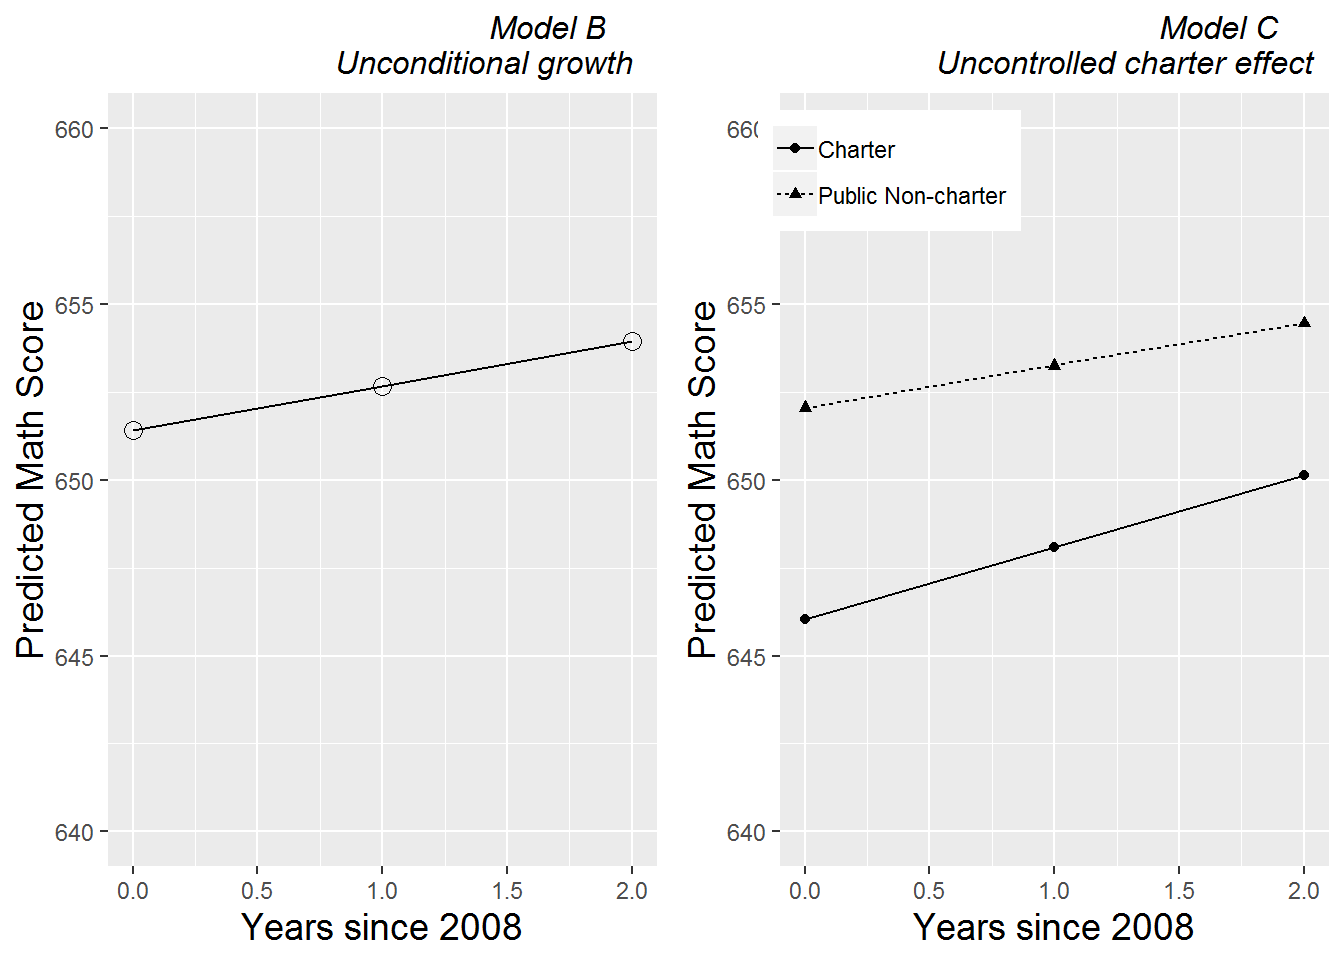
\includegraphics[width=0.6\linewidth]{bookdown-bysh_files/figure-latex/lon-scat4-1} 

}

\caption{ Fitted growth curves for Models B and C.}\label{fig:lon-scat4}
\end{figure}

\hypertarget{modeld}{%
\subsection{Add percent free and reduced lunch as a covariate}\label{modeld}}

Although we will still be primarily interested in the effect of school type on both 2008 test scores and rate of change in test scores (as we observed in Model C), we can try to improve our estimates of school type effects through the introduction of meaningful covariates. In this study, we are particularly interested in Level Two covariates---those variables which differ by school but which remain basically constant for a given school over time---such as urban or rural location, percentage of special education students, and percentage of students with free and reduced lunch. In Section \ref{twostage9}, we investigated the relationship between percent free and reduced lunch and a school's test score in 2008 and their rate of change from 2008 to 2010.

Based on these analyses, we will begin by adding percent free and reduced lunch as a Level Two predictor for both intercept and slope (Model D):

\begin{itemize}
\item
  Level One:
  \begin{equation*}
  Y_{ij}=a_{i} + b_{i}\textrm{Year08}_{ij} + \epsilon_{ij}
  \end{equation*}
\item
  Level Two:
  \begin{align*}
  a_{i} & = \alpha_{0} + \alpha_{1}\textrm{Charter}_i + \alpha_{2}\textrm{schpctfree}_i + u_{i}\\
  b_{i} & = \beta_{0} + \beta_{1}\textrm{Charter}_i + \beta_{2}\textrm{schpctfree}_i + v_{i}
  \end{align*}
\end{itemize}

The composite model is then:

\begin{align*}
Y_{ij}= [\alpha_{0}&+\alpha_{1}\textrm{Charter}_i +\alpha_{2}\textrm{schpctfree}_i + \beta_{0}\textrm{Year08}_{ij} \nonumber \\
 &+ \beta_{1}\textrm{Charter}_i\textrm{Year08}_{ij}  + \beta_{2}\textrm{schpctfree}_i\textrm{Year08}_{ij}] \nonumber \\ 
 &+ [u_{i} + v_{i}\textrm{Year08}_{ij} + \epsilon_{ij}]
\end{align*}
where error terms are defined as in Model C.

\begin{Shaded}
\begin{Highlighting}[]
\CommentTok{#Model D2 (Introduce SchPctFree at level 2)}
\NormalTok{model.d2 <-}\StringTok{ }\KeywordTok{lmer}\NormalTok{(MathAvgScore}\OperatorTok{~}\StringTok{ }\NormalTok{charter }\OperatorTok{+}\StringTok{ }\NormalTok{SchPctFree }\OperatorTok{+}\StringTok{ }\NormalTok{year08 }\OperatorTok{+}\StringTok{ }
\StringTok{  }\NormalTok{charter}\OperatorTok{:}\NormalTok{year08 }\OperatorTok{+}\StringTok{ }\NormalTok{SchPctFree}\OperatorTok{:}\NormalTok{year08 }\OperatorTok{+}\StringTok{ }\NormalTok{(year08}\OperatorTok{|}\NormalTok{schoolid),}
  \DataTypeTok{REML=}\NormalTok{T, }\DataTypeTok{data=}\NormalTok{chart.long)}
\end{Highlighting}
\end{Shaded}

\begin{verbatim}
##  Groups   Name        Variance Std.Dev. Corr
##  schoolid (Intercept) 19.13    4.37         
##           year08       0.16    0.40     0.51
##  Residual              8.80    2.97
\end{verbatim}

\begin{verbatim}
##  Number of Level Two groups =  618
\end{verbatim}

\begin{verbatim}
##                    Estimate Std. Error  t value
## (Intercept)       659.27848   0.444690 1482.558
## charter            -3.43994   0.712836   -4.826
## SchPctFree         -0.16654   0.008907  -18.697
## year08              1.64137   0.189499    8.662
## charter:year08      0.98076   0.318583    3.078
## SchPctFree:year08  -0.01041   0.003839   -2.711
\end{verbatim}

\begin{verbatim}
##  AIC =  9988 ;  BIC =  10043
\end{verbatim}

\begin{Shaded}
\begin{Highlighting}[]
\NormalTok{drop_in_dev <-}\StringTok{ }\KeywordTok{anova}\NormalTok{(model.d2, model.c, }\DataTypeTok{test =} \StringTok{"Chisq"}\NormalTok{)}
\end{Highlighting}
\end{Shaded}

\begin{verbatim}
         npar   AIC   BIC logLik   dev Chisq Df
model.c     8 10305 10348  -5144 10289    NA NA
model.d2   10  9967 10022  -4974  9947 341.5  2
              pval
model.c         NA
model.d2 7.158e-75
\end{verbatim}

Compared to Model C, the introduction of school-level poverty based on percentage of students receiving free and reduced lunch in Model D leads to similar conclusions about the significance of the charter school effect on both the intercept and the slope, although the magnitude of these estimates change after controlling for poverty levels. The estimated gap in test scores between charter and non-charter schools in 2008 is smaller in Model D, while estimates of improvement between 2008 and 2010 increase for both types of schools. Inclusion of free and reduced lunch reduces the unexplained variability between schools in 2008 math scores by 27\%, while unexplained variability in rates of change between schools again increases slightly based on pseudo \(R^2\) values. A \textbf{likelihood ratio test} using maximum likelihood estimates illustrates that adding free and reduced lunch as a Level Two covariate significantly improves our model (\(\chi^2 = 341.5, df=2, p<.001\)). Specific fixed effect parameter estimates are given below:

\begin{itemize}
\item
  \(\hat{\alpha}_{0}= 659.3.\) The estimated mean math test score for 2008 is 659.3 for non-charter public schools with no students receiving free and reduced lunch.
\item
  \(\hat{\alpha}_{1}= -3.44.\) Charter schools have an estimated mean math test score in 2008 which is 3.44 points lower than non-charter public schools, controlling for effects of school-level poverty.
\item
  \(\hat{\alpha}_{2}= -0.17.\) Each 10\% increase in the percentage of students at a school receiving free and reduced lunch is associated with a 1.7 point decrease in mean math test scores for 2008, after controlling for school type.
\item
  \(\hat{\beta}_{0}= 1.64.\) Public non-charter schools with no students receiving free and reduced lunch have an estimated mean increase in math test score of 1.64 points per year during the three years of observation.
\item
  \(\hat{\beta}_{1}= 0.98.\) Charter schools have an estimated mean yearly increase in math test scores over the three year observation period of 2.62, which is 0.98 points higher than the annual increase for public non-charter schools, after controlling for school-level poverty.
\item
  \(\hat{\beta}_{2}= -0.010.\) Each 10\% increase in the percentage of students at a school receiving free and reduced lunch is associated with a 0.10 point decrease in rate of change over the three years of observation, after controlling for school type.
\end{itemize}

\hypertarget{modelf9}{%
\subsection{A potential final model with three Level Two covariates}\label{modelf9}}

We now begin iterating toward a ``final model'' for these data, on which we will base conclusions. Being cognizant of typical features of a ``final model'' as outlined in Chapter \ref{ch-multilevelintro}, we offer one possible final model for this data---Model F:

\begin{itemize}
\tightlist
\item
  Level One:
\end{itemize}

\begin{equation*}
Y_{ij}= a_{i} + b_{i}\textrm{Year08}_{ij} + \epsilon_{ij}
\end{equation*}

\begin{itemize}
\tightlist
\item
  Level Two:
\end{itemize}

\begin{align*}
a_{i} & = \alpha_{0} + \alpha_{1}\textrm{Charter}_i + \alpha_{2}\textrm{urban}_i + \alpha_{3}\textrm{schpctsped}_i + \alpha_{4}\textrm{schpctfree}_i + u_{i} \\
b_{i} & = \beta_{0} + \beta_{1}\textrm{Charter}_i + \beta_{2}\textrm{urban}_i + \beta_{3}\textrm{schpctsped}_i + v_{i}
\end{align*}

where we find the effect of charter schools on 2008 test scores after adjusting for urban or rural location, percentage of special education students, and percentage of students that receive free or reduced lunch, and the effect of charter schools on yearly change between 2008 and 2010 after adjusting for urban or rural location and percentage of special education students. We can use AIC and BIC criteria to compare Model F with Model D, since the two models are not nested. By both criteria, Model F is significantly better than Model D: AIC of 9885 vs.~9988, and BIC of 9956 vs.~10043. Based on the R output below, we offer interpretations for estimates of model fixed effects:

\begin{Shaded}
\begin{Highlighting}[]
\NormalTok{model.f2 <-}\StringTok{ }\KeywordTok{lmer}\NormalTok{(MathAvgScore }\OperatorTok{~}\StringTok{ }\NormalTok{charter }\OperatorTok{+}\StringTok{ }\NormalTok{urban }\OperatorTok{+}\StringTok{ }\NormalTok{SchPctFree }\OperatorTok{+}\StringTok{ }
\StringTok{  }\NormalTok{SchPctSped }\OperatorTok{+}\StringTok{ }\NormalTok{charter}\OperatorTok{:}\NormalTok{year08 }\OperatorTok{+}\StringTok{ }\NormalTok{urban}\OperatorTok{:}\NormalTok{year08 }\OperatorTok{+}\StringTok{ }
\StringTok{  }\NormalTok{SchPctSped}\OperatorTok{:}\NormalTok{year08 }\OperatorTok{+}\StringTok{ }\NormalTok{year08 }\OperatorTok{+}
\StringTok{  }\NormalTok{(year08}\OperatorTok{|}\NormalTok{schoolid), }\DataTypeTok{REML=}\NormalTok{T, }\DataTypeTok{data=}\NormalTok{chart.long)}
\end{Highlighting}
\end{Shaded}

\begin{verbatim}
##  Groups   Name        Variance Std.Dev. Corr
##  schoolid (Intercept) 16.94756 4.1167       
##           year08       0.00475 0.0689   0.85
##  Residual              8.82197 2.9702
\end{verbatim}

\begin{verbatim}
##  Number of Level Two groups =  618
\end{verbatim}

\begin{verbatim}
##                    Estimate Std. Error  t value
## (Intercept)       661.01042   0.512888 1288.800
## charter            -3.22286   0.698547   -4.614
## urban              -1.11383   0.427566   -2.605
## SchPctFree         -0.15281   0.008096  -18.874
## SchPctSped         -0.11770   0.020612   -5.710
## year08              2.14430   0.200867   10.675
## charter:year08      1.03087   0.315159    3.271
## urban:year08       -0.52749   0.186480   -2.829
## SchPctSped:year08  -0.04674   0.010166   -4.598
\end{verbatim}

\begin{verbatim}
##  AIC =  9885 ;  BIC =  9956
\end{verbatim}

\begin{itemize}
\tightlist
\item
  \(\hat{\alpha}_{0}= 661.0.\) The estimated mean math test score for 2008 is 661.0 for public schools in rural areas with no students qualifying for special education or free and reduced lunch.
\item
  \(\hat{\alpha}_{1}= -3.22.\) Charter schools have an estimated mean math test score in 2008 which is 3.22 points lower than non-charter public schools, after controlling for urban or rural location, percent special education, and percent free and reduced lunch.
\item
  \(\hat{\alpha}_{2}= -1.11.\) Schools in urban areas have an estimated mean math score in 2008 which is 1.11 points lower than schools in rural areas, after controlling for school type, percent special education, and percent free and reduced lunch.
\item
  \(\hat{\alpha}_{3}= -0.118.\) A 10\% increase in special education students at a school is associated with a 1.18 point decrease in estimated mean math score for 2008, after controlling for school type, urban or rural location, and percent free and reduced lunch.
\item
  \(\hat{\alpha}_{4}= -0.153.\) A 10\% increase in free and reduced lunch students at a school is associated with a 1.53 point decrease in estimated mean math score for 2008, after controlling for school type, urban or rural location, and percent special education.
\item
  \(\hat{\beta}_{0}= 2.14.\) Public non-charter schools in rural areas with no students qualifying for special education have an estimated increase in mean math test score of 2.14 points per year over the three year observation period, after controlling for percent of students receiving free and reduced lunch.
\item
  \(\hat{\beta}_{1}= 1.03.\) Charter schools have an estimated mean annual increase in math score that is 1.03 points higher than public non-charter schools over the three year observation period, after controlling for urban or rural location, percent special education, and percent free and reduced lunch.
\item
  \(\hat{\beta}_{2}= -0.53.\) Schools in urban areas have an estimated mean annual increase in math score that is 0.53 points lower than schools from rural areas over the three year observation period, after controlling for school type, percent special education, and percent free and reduced lunch.
\item
  \(\hat{\beta}_{3}= -0.047.\) A 10\% increase in special education students at a school is associated with an estimated mean annual increase in math score that is 0.47 points lower over the three year observation period, after controlling for school type, urban or rural location, and percent free and reduced lunch.
\end{itemize}

From this model, we again see that 2008 sixth grade math test scores from charter schools were significantly lower than similar scores from public non-charter schools, after controlling for school location and demographics. However, charter schools showed significantly greater improvement between 2008 and 2010 compared to public non-charter schools, although charter school test scores were still lower than public school scores in 2010, on average. We also tested several interactions between Level Two covariates and charter schools and found none to be significant, indicating that the 2008 gap between charter schools and public non-charter schools was consistent across demographic subgroups. The faster improvement between 2008 and 2010 for charter schools was also consistent across demographic subgroups (found by testing three-way interactions). Controlling for school location and demographic variables provided more reliable and nuanced estimates of the effects of charter schools, while also providing interesting insights. For example, schools in rural areas not only had higher test scores than schools in urban areas in 2008, but the gap grew larger over the study period given fixed levels of percent special education, percent free and reduced lunch, and school type. In addition, schools with higher levels of poverty lagged behind other schools and showed no signs of closing the gap, and schools with higher levels of special education students had both lower test scores in 2008 and slower rates of improvement during the study period, again given fixed levels of other covariates.

As we demonstrated in this case study, applying multilevel methods to two-level longitudinal data yields valuable insights about our original research questions while properly accounting for the structure of the data.

\hypertarget{longitudinal-paraboot}{%
\subsection{Parametric bootstrap testing}\label{longitudinal-paraboot}}

We could further examine whether or not a simplified version of Model F, with fewer random effects, might be preferable. For instance, consider testing whether we could remove \(v_i\) in Model F in Section \ref{modelf9}, to create Model F0. Removing \(v_i\) is equivalent to setting \(\sigma_{v}^{2} = 0\) and \(\rho_{uv} = 0\). We begin by comparing Model F (full model) to Model F0 (reduced model) using a likelihood ratio test:

\begin{Shaded}
\begin{Highlighting}[]
\CommentTok{#Model F0 (remove 2 variance components from Model F)}
\NormalTok{model.f0 <-}\StringTok{ }\KeywordTok{lmer}\NormalTok{(MathAvgScore }\OperatorTok{~}\StringTok{ }\NormalTok{charter }\OperatorTok{+}\StringTok{ }\NormalTok{urban }\OperatorTok{+}\StringTok{ }\NormalTok{SchPctFree }\OperatorTok{+}\StringTok{ }
\StringTok{  }\NormalTok{SchPctSped }\OperatorTok{+}\StringTok{ }\NormalTok{charter}\OperatorTok{:}\NormalTok{year08 }\OperatorTok{+}\StringTok{ }\NormalTok{urban}\OperatorTok{:}\NormalTok{year08 }\OperatorTok{+}\StringTok{ }
\StringTok{  }\NormalTok{SchPctSped}\OperatorTok{:}\NormalTok{year08 }\OperatorTok{+}\StringTok{ }\NormalTok{year08 }\OperatorTok{+}
\StringTok{  }\NormalTok{(}\DecValTok{1}\OperatorTok{|}\NormalTok{schoolid), }\DataTypeTok{REML=}\NormalTok{T, }\DataTypeTok{data=}\NormalTok{chart.long)}
\end{Highlighting}
\end{Shaded}

\begin{verbatim}
##  Groups   Name        Variance Std.Dev.
##  schoolid (Intercept) 17.46    4.18    
##  Residual              8.83    2.97
\end{verbatim}

\begin{verbatim}
##  Number of Level Two groups =  618
\end{verbatim}

\begin{verbatim}
##                    Estimate Std. Error  t value
## (Intercept)       661.02599    0.51691 1278.813
## charter            -3.21918    0.70543   -4.563
## urban              -1.11852    0.43204   -2.589
## SchPctFree         -0.15302    0.00810  -18.892
## SchPctSped         -0.11813    0.02080   -5.680
## year08              2.13924    0.20097   10.644
## charter:year08      1.03157    0.31551    3.270
## urban:year08       -0.52330    0.18651   -2.806
## SchPctSped:year08  -0.04645    0.01017   -4.568
\end{verbatim}

\begin{verbatim}
##  AIC =  9881 ;  BIC =  9941
\end{verbatim}

\begin{Shaded}
\begin{Highlighting}[]
\NormalTok{drop_in_dev <-}\StringTok{ }\KeywordTok{anova}\NormalTok{(model.f2, model.f0, }\DataTypeTok{test =} \StringTok{"Chisq"}\NormalTok{)}
\end{Highlighting}
\end{Shaded}

\begin{verbatim}
         npar  AIC  BIC logLik  dev  Chisq Df   pval
model.f0   11 9854 9914  -4916 9832     NA NA     NA
model.f2   13 9857 9928  -4916 9831 0.3376  2 0.8447
\end{verbatim}

When testing random effects at the boundary (such as \(\sigma_{v}^{2} = 0\)) or those with restricted ranges (such as \(\rho_{uv} = 0\)), using a chi-square distribution to conduct a likelihood ratio test is not appropriate. In fact, this will produce a conservative test, with p-values that are too large and not rejected enough (\citet{Bryk2002}, \citet{Singer2003}, \citet{Faraway2005}). For example, we should suspect that the p-value (.8447) produced by the likelihood ratio test comparing Models F and F0 is too large, that the real probability of getting a likelihood ratio test statistic of 0.3376 or greater when Model F0 is true is smaller than .8447.

Researchers often use methods like the \textbf{parametric bootstrap} \index{parametric bootstrap} to better approximate the distribution of the likelihood test statistic and produce more accurate p-values by simulating data under the null hypothesis. Here are the basic steps for running a parametric bootstrap procedure to compare Model F0 with Model F (see associated diagram in Figure \ref{fig:parabootdiagram}):

\begin{itemize}
\tightlist
\item
  Fit Model F0 (the null model) to obtain estimated fixed effects and variance components (this is the ``parametric'' part.)
\item
  Use the estimated fixed effects and variance components from the null model to regenerate a new set of math test scores with the same sample size (\(n=1733\)) and associated covariates for each observation as the original data (this is the ``bootstrap'' part.)
\item
  Fit both Model F0 (the reduced model) and Model F (the full model) to the new data
\item
  Compute a likelihood ratio statistic comparing Models F0 and F
\item
  Repeat the previous 3 steps many times (e.g., 1000)
\item
  Produce a histogram of likelihood ratio statistics to illustrate its behavior when the null hypothesis is true
\item
  Calculate a p-value by finding the proportion of times the bootstrapped test statistic is greater than our observed test statistic
\end{itemize}

\begin{figure}
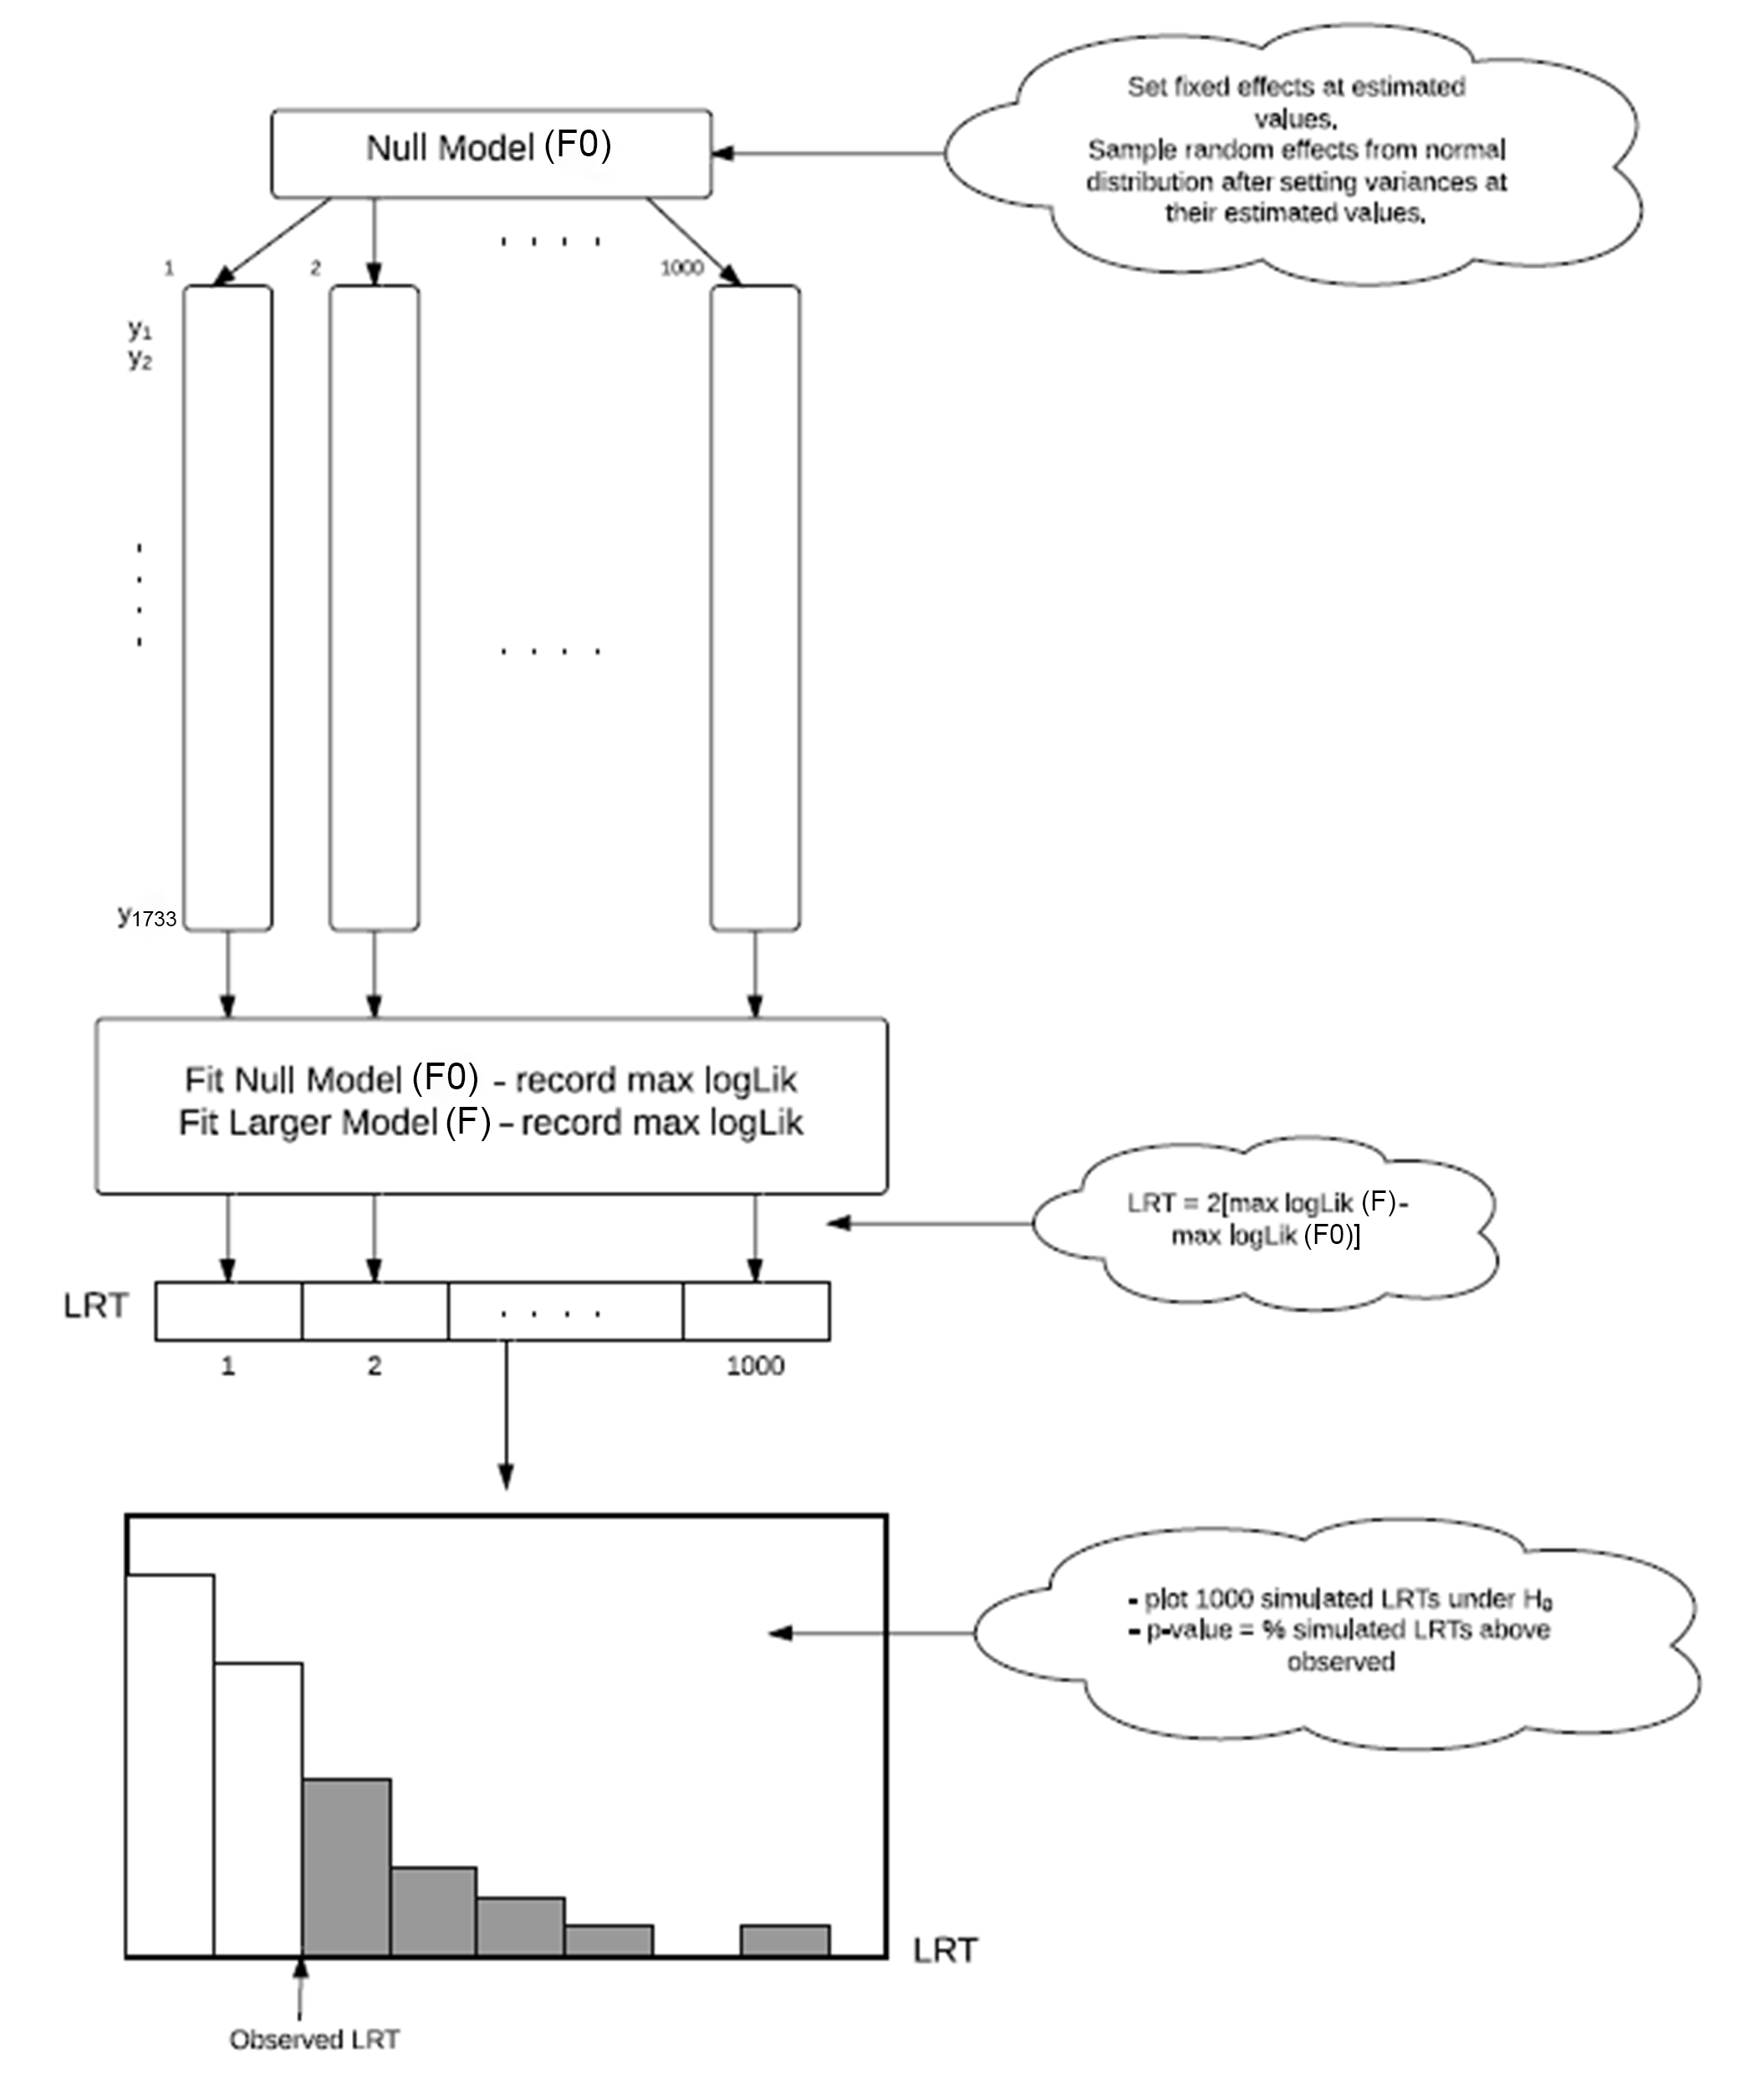
\includegraphics[width=0.8\linewidth]{data/ParametricBootstrapDiagram} \caption{The steps in conducting a parametric bootstrap test comparing Models F and F0.}\label{fig:parabootdiagram}
\end{figure}

Let's see how new test scores are generated under the parametric bootstrap. Consider, for instance, \(i=1\) and \(j=1,2,3\); that is, consider test scores for School \#1 (Rippleside Elementary) across all three years (2008, 2009, and 2010). Table \ref{tab:rippleside} shows the original data for Rippleside Elementary.

\begin{table}

\caption{\label{tab:rippleside}Original data for Rippleside Elementary (School 1)}
\centering
\resizebox{\linewidth}{!}{
\begin{tabular}[t]{lrrrrrr}
\toprule
schoolName & urban & charter & schPctsped & schPctfree & year08 & MathAvgScore\\
\midrule
RIPPLESIDE ELEMENTARY & 0 & 0 & 0.1176 & 0.3627 & 0 & 652.8\\
RIPPLESIDE ELEMENTARY & 0 & 0 & 0.1176 & 0.3627 & 1 & 656.6\\
RIPPLESIDE ELEMENTARY & 0 & 0 & 0.1176 & 0.3627 & 2 & 652.6\\
\bottomrule
\end{tabular}}
\end{table}

\textbf{Level Two}

One way to see the data generation process under the null model (Model F0) is to start with Level Two and work backwards to Level One. Recall that our Level Two models for \(a_{i}\) and \(b_{i}\), the true intercept and slope for school \(i\), in Model F0 are:

\begin{align*}
a_{i} & = \alpha_{0} + \alpha_{1}\textrm{Charter}_i + \alpha_{2}\textrm{urban}_i + \alpha_{3}\textrm{schpctsped}_i + \alpha_{4}\textrm{schpctfree}_i + u_{i} \\
b_{i} & = \beta_{0} + \beta_{1}\textrm{Charter}_i + \beta_{2}\textrm{urban}_i + \beta_{3}\textrm{schpctsped}_i
\end{align*}

All the \(\alpha\) and \(\beta\) terms will be fixed at their estimated values, so the one term that will change for each bootstrapped data set is \(u_{i}\). As we obtain a numeric value for \(u_{i}\) for each school, we will fix the subscript. For example, if \(u_{i}\) is set to -5.92 for School \#1, then we would denote this by \(u_{1}=-5.92\). Similarly, in the context of Model F0, \(a_{1}\) represents the 2008 math test score for School \#1, where \(u_{1}\) quantifies how School \#1's 2008 score differs from the average 2008 score across all schools with the same attributes: charter status, urban or rural location, percent of special education students, and percent of free and reduced lunch students.

According to Model F0, each \(u_{i}\) is sampled from a normal distribution with mean 0 and standard deviation 4.18. That is, a random component to the intercept for School \#1 (\(u_{1}\)) would be sampled from a normal distribution with mean 0 and SD 4.18; say, for instance, \(u_{1}=-5.92\). We would sample \(u_{2},...,u_{618}\) in a similar manner for all 618 schools. Then we can produce a model-based intercept and slope for School \#1:

\begin{align*}
a_{1} & = 661.03-3.22(0)-1.12(0)-0.12(11.8)-0.15(36.3)-5.92 = 648.2 \\
b_{1} & = 2.14+1.03(0)-0.52(0)-.046(11.8) = 1.60
\end{align*}

Notice a couple of features of the above derivations. First, all of the coefficients from the above equations (\(\alpha_{0}=661.03\), \(\alpha_{1}=-3.22\), etc.) come from the estimated fixed effects from Model F0. Second, ``public non-charter'' is the reference level for \texttt{charter} and ``rural'' is the reference level for \texttt{urban}, so both of those predictors are 0 for Rippleside Elementary. Third, the mean intercept (2008 test scores) for schools like Rippleside that are rural and public non-charter, with 11.8\% special education students and 36.3\% free and reduced lunch students, is 661.03 - 0.12(11.8) - 0.15(36.3) = 654.2. The mean yearly improvement in test scores for rural, public non-charter schools with 11.8\% special education students is then 1.60 points per year (2.14 - .046*11.8). School \#1 (Rippleside) therefore has a 2008 test score that is 5.92 points below the mean for all similar schools, but every such school is assumed to have the same improvement rate in test scores of 1.60 points per year because of our assumption that there is no school-to-school variability in yearly rate of change (i.e., \(v_{i}=0\)).

\textbf{Level One}

We next proceed to Level One, where the scores from Rippleside are modeled as a linear function of year (\(654.2 + 1.60\textrm{Year08}_{ij}\)) with a normally distributed residual \(\epsilon_{1k}\) at each time point \(k\). Three residuals (one for each year) are sampled independently from a normal distribution with mean 0 and standard deviation 2.97 -- the standard deviation again coming from parameter estimates from fitting Model F0 to the actual data. Suppose we obtain residuals of \(\epsilon_{11}=-3.11\), \(\epsilon_{12}=1.19\), and \(\epsilon_{13}=2.41\). In that case, our parametrically generated data for Rippleside Elementary (School \#1) would look like:

\[ \begin{array}{rcccl}
   Y_{11} & = & 654.2+1.60(0)-3.11 & = & 651.1 \\
   Y_{12} & = & 654.2+1.60(1)+1.19 & = & 657.0 \\
   Y_{13} & = & 654.2+1.60(2)+2.41 & = & 659.8 \\
   \end{array} \]

We would next turn to School \#2 (\(i=2\))---Wrenshall Elementary. Fixed effects would remain the same but covariates would change, as Wrenshall has 15.2\% special education students and 42.4\% free and reduced lunch students. We would, however, sample a new residual \(u_{2}\) at Level Two, producing a different intercept \(a_{2}\) than observed for School \#1. Three new independent residuals \(\epsilon_{2k}\) would also be selected at Level One, from the same normal distribution as before with mean 0 and standard deviation 2.97.

Once an entire set of simulated scores for every school and year have been generated based on Model F0, two models are fit to this data:

\begin{itemize}
\tightlist
\item
  Model F0 -- the correct (null) model that was actually used to generate the responses
\item
  Model F -- the incorrect (full) model that contains two extra variance components -- \(\sigma_{v}^{2}\) and \(\sigma_{uv}\) -- that were not actually used when generating the responses
\end{itemize}

\begin{Shaded}
\begin{Highlighting}[]
\CommentTok{# Generate 1 set of bootstrapped data and run chi-square test}
\CommentTok{#  (will also work if use REML models, but may take longer)}
\KeywordTok{set.seed}\NormalTok{(}\DecValTok{3333}\NormalTok{)}
\NormalTok{d <-}\StringTok{ }\KeywordTok{drop}\NormalTok{(}\KeywordTok{simulate}\NormalTok{(model.f0ml))}
\NormalTok{m2 <-}\KeywordTok{refit}\NormalTok{(model.f2ml, }\DataTypeTok{newresp=}\NormalTok{d)}
\NormalTok{m1 <-}\KeywordTok{refit}\NormalTok{(model.f0ml, }\DataTypeTok{newresp=}\NormalTok{d)}
\NormalTok{drop_in_dev <-}\StringTok{ }\KeywordTok{anova}\NormalTok{(m2, m1, }\DataTypeTok{test =} \StringTok{"Chisq"}\NormalTok{)}
\end{Highlighting}
\end{Shaded}

\begin{verbatim}
   npar  AIC  BIC logLik  dev Chisq Df   pval
m1   11 9891 9951  -4935 9869    NA NA     NA
m2   13 9891 9962  -4932 9865 4.581  2 0.1012
\end{verbatim}

A likelihood ratio test statistic is calculated comparing Model F0 to Model F. For example, after continuing as above to generate new \(Y_{ij}\) values corresponding to all 1733 score observations, we fit both models to the ``bootstrapped'' data. Since the data was generated using Model F0, we would expect the two extra terms in Model F (\(\sigma^2_{v}\) and \(\sigma_{uv}\)) to contribute very little to the quality of the fit; Model F will have a slightly larger likelihood and loglikelihood since it contains every parameter from Model F0 plus two more, but the difference in the likelihoods should be due to chance. In fact, that is what the output above shows. Model F does have a larger loglikelihood than Model F0 (-4932 vs.~-4935), but this small difference is not statistically significant based on a chi-square test with 2 degrees of freedom (p=.1012).

However, we are really only interested in saving the likelihood ratio test statistic from this bootstrapped sample (\(2*(-4932 - (-4935) = 4.581\)). By generating (``bootstrapping'') many sets of responses based on estimated parameters from Model F0 and calculating many likelihood ratio test statistics, we can observe how this test statistic behaves under the null hypothesis of \(\sigma_{v}^{2} = \sigma_{uv} = 0\), rather than making the (dubious) assumption that its behavior is described by a chi-square distribution with 2 degrees of freedom. Figure \ref{fig:paraboot9} illustrates the null distribution of the likelihood ratio test statistic derived by the parametric bootstrap procedure as compared to a chi-square distribution. A p-value for comparing our full and reduced models can be approximated by finding the proportion of likelihood ratio test statistics generated under the null model which exceed our observed likelihood ratio test (0.3376). The parametric bootstrap provides a more reliable p-value in this case (.578 from table below); a chi-square distribution puts too much mass in the tail and not enough near 0, leading to overestimation of the p-value. Based on this test, we would still choose our simpler Model F0.

\begin{Shaded}
\begin{Highlighting}[]
\KeywordTok{bootstrapAnova}\NormalTok{(}\DataTypeTok{mA=}\NormalTok{model.f2ml, }\DataTypeTok{m0=}\NormalTok{model.f0ml, }\DataTypeTok{B=}\DecValTok{1000}\NormalTok{)}
\end{Highlighting}
\end{Shaded}

\begin{verbatim}
   npar logLik  dev  Chisq Df pval_boot
m0   11  -4916 9832     NA NA        NA
mA   13  -4916 9831 0.3376  2     0.578
\end{verbatim}

\begin{figure}

{\centering 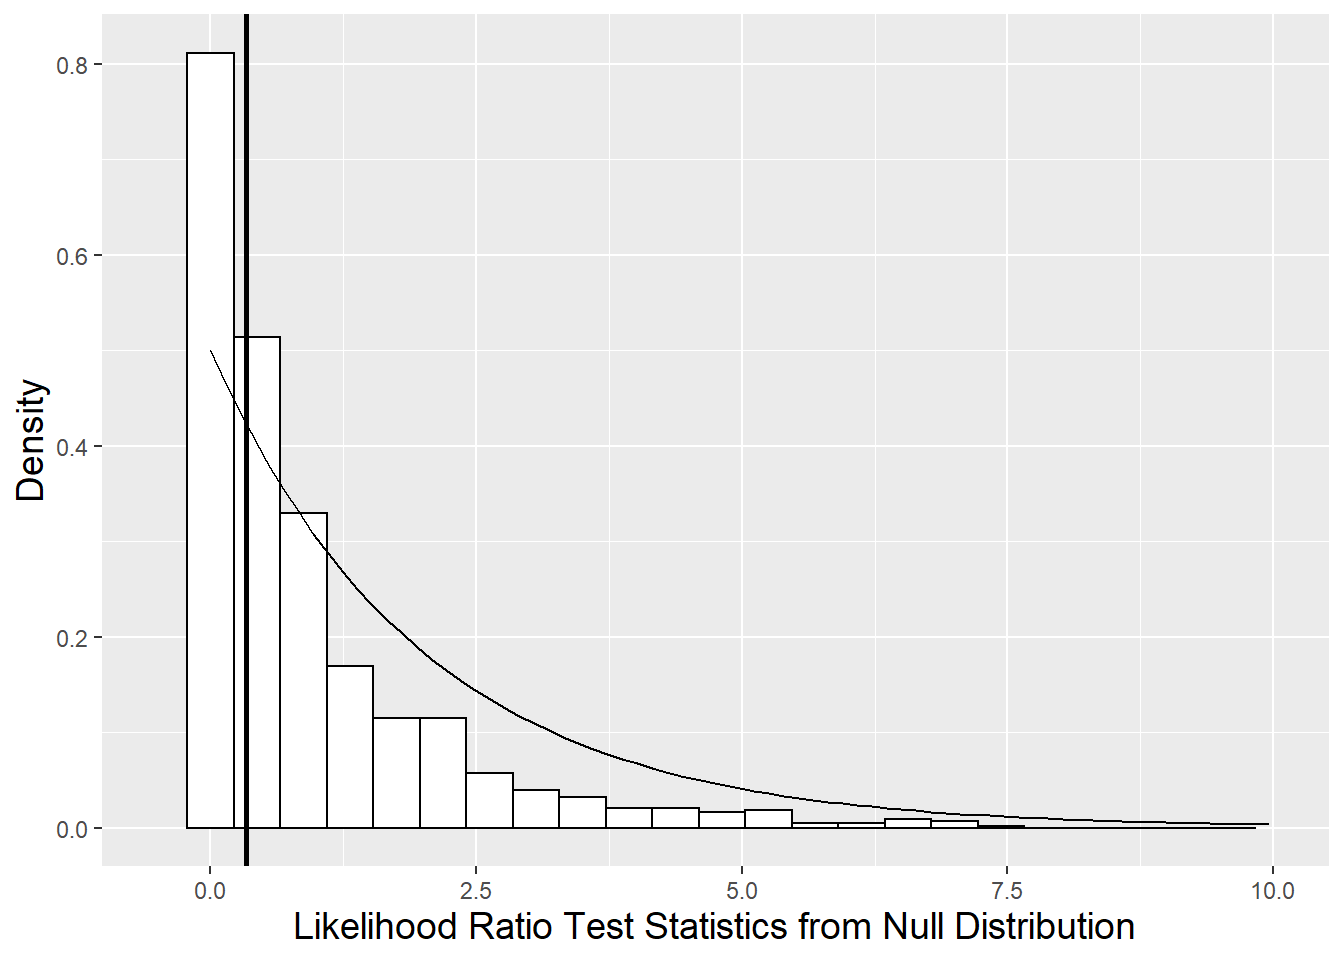
\includegraphics[width=0.6\linewidth]{bookdown-bysh_files/figure-latex/paraboot9-1} 

}

\caption{Null distribution of likelihood ratio test statistic derived using parametric bootstrap (histogram) compared to a chi-square distribution with 2 degrees of freedom (smooth curve).  The horizontal line represents the observed likelihood ratio test statistic.}\label{fig:paraboot9}
\end{figure}

Another way of examining whether or not we should stick with the reduced model or reject it in favor of the larger model is by generating parametric bootstrap samples, and then using those samples to produce 95\% confidence intervals for both \(\rho_{uv}\) and \(\sigma_{v}\).

\begin{Shaded}
\begin{Highlighting}[]
\NormalTok{bootciF =}\StringTok{ }\KeywordTok{confint}\NormalTok{(model.f2, }\DataTypeTok{method=}\StringTok{"boot"}\NormalTok{, }\DataTypeTok{oldNames=}\NormalTok{F)}
\NormalTok{bootciF}
\end{Highlighting}
\end{Shaded}

\begin{verbatim}
##                                      2.5 %    97.5 %
## sd_(Intercept)|schoolid           3.801826   4.50866
## cor_year08.(Intercept)|schoolid  -1.000000   1.00000
## sd_year08|schoolid                0.009203   0.91060
## sigma                             2.779393   3.07776
## (Intercept)                     660.071996 662.04728
## charter                          -4.588611  -2.07372
## urban                            -2.031600  -0.29152
## SchPctFree                       -0.169426  -0.13738
## SchPctSped                       -0.156065  -0.07548
## year08                            1.722458   2.56106
## charter:year08                    0.449139   1.65928
## urban:year08                     -0.905941  -0.17156
## SchPctSped:year08                -0.066985  -0.02617
\end{verbatim}

From the output above, the 95\% bootstrapped confidence interval for \(\rho_{uv}\) (-1, 1) contains 0, and the interval for \(\sigma_{v}\) (0.0092, 0.9106) nearly contains 0, providing further evidence that the larger model is not needed.

In this section, we have offered the parametric bootstrap as a noticeable improvement over the likelihood ratio test with an approximate chi-square distribution for testing random effects, especially those near a boundary. Typically when we conduct hypothesis tests involving variance terms we are testing at the boundary, since we are asking if the variance term is really necessary (i.e., \(H_0: \sigma^2=0\) vs.~\(H_A: \sigma^2 > 0\)). However, what if we are conducting a hypothesis test about a fixed effect? For the typical test of whether or not a fixed effect is significant -- e.g., \(H_0: \alpha_i=0\) vs.~\(H_A: \alpha_i \neq 0\) -- we are \emph{not} testing at the boundary, since most fixed effects have no bounds on allowable values. We have often used a likelihood ratio test with an approximate chi-square distribution in these settings -- does that provide accurate p-values? Although some research (e.g., \citet{Faraway2005}) shows that p-values of fixed effects from likelihood ratio tests can tend to be anti-conservative (too low), in general the approximation is not bad. We will continue to use the likelihood ratio test with a chi-square distribution for fixed effects, but you could always check your p-values using a parametric bootstrap approach.

\hypertarget{errorcovariance}{%
\section{Covariance structure among observations}\label{errorcovariance}}

Part of our motivation for framing our model for multilevel data was to account for the correlation among observations made on the same school (the Level Two observational unit). Our two-level model, through error terms on both Level One and Level Two variables, actually implies a specific within-school covariance structure \index{covariance structure} among observations, yet we have not (until now) focused on this imposed structure. For example:

\begin{itemize}
\tightlist
\item
  What does our two-level model say about the relative variability of 2008 and 2010 scores from the same school?
\item
  What does it say about the correlation between 2008 and 2009 scores from the same school?
\end{itemize}

In this section, we will describe the within-school covariance structure imposed by our two-level model and offer alternative covariance structures that we might consider, especially in the context of longitudinal data. In short, we will discuss how we might decide if our implicit covariance structure in our two-level model is satisfactory for the data at hand. Then, in the succeeding optional section, we provide derivations of the imposed within-school covariance structure for our standard two-level model using results from probability theory.

\hypertarget{standarderror}{%
\subsection{Standard covariance structure}\label{standarderror}}

We will use Model C (uncontrolled effects of school type) to illustrate covariance structure within subjects. Recall that, in composite form, Model C is:

\begin{align*}
Y_{ij} & = a_{i}+b_{i}\textrm{Year08}_{ij}+ \epsilon_{ij} \\
       & = (\alpha_{0}+ \alpha_{1}\textrm{Charter}_i + u_{i}) + (\beta_{0}+\beta_{1}\textrm{Charter}_i +v_{i}) \textrm{Year08}_{ij} + \epsilon_{ij} \\
       & = [\alpha_{0}+\alpha_{1}\textrm{Charter}_i + \beta_{0}\textrm{Year08}_{ij} + \beta_{1}\textrm{Charter}_i\textrm{Year08}_{ij}] + [u_{i} \\
       & \quad + v_{i}\textrm{Year08}_{ij} + \epsilon_{ij}]
\end{align*}
\noindent where \(\epsilon_{ij}\sim N(0,\sigma^2)\) and

\[ \left[ \begin{array}{c}
            u_{i} \\ v_{i}
          \end{array}  \right] \sim N \left( \left[
          \begin{array}{c}
            0 \\ 0
          \end{array} \right], \left[
          \begin{array}{cc}
            \sigma_{u}^{2} & \\
            \sigma_{uv} & \sigma_{v}^{2}
          \end{array} \right] \right) . \]

For School \(i\), the covariance structure for the three time points has general form:

\[ Cov(\mathbf{Y}_i) =  \left[
          \begin{array}{cccc}
            Var(Y_{i1}) & Cov(Y_{i1},Y_{i2}) & Cov(Y_{i1},Y_{i3}) \\
            Cov(Y_{i1},Y_{i2}) & Var(Y_{i2}) & Cov(Y_{i2},Y_{i3}) \\
            Cov(Y_{i1},Y_{i3}) & Cov(Y_{i2},Y_{i3}) & Var(Y_{i3})
          \end{array} \right] \]
where, for instance, \(Var(Y_{i1})\) is the variability in 2008 test scores (time \(j=1\)), \(Cov(Y_{i1},Y_{i2})\) is the covariance between 2008 and 2009 test scores (times \(j=1\) and \(j=2\)), etc. Since covariance measures the tendency of two variables to move together, we expect positive values for all three covariance terms in \(Cov(\mathbf{Y}_i)\), since schools with relatively high test scores in 2008 are likely to also have relatively high test scores in 2009 or 2010. The correlation between two variables then scales covariance terms to values between -1 and 1, so by the same rationale, we expect correlation coefficients between two years to be near 1. If observations within school were independent---that is, knowing a school had relatively high scores in 2008 tells nothing about whether that school will have relatively high scores in 2009 or 2010---then we would expect covariance and correlation values near 0.

It is important to notice that the error structure at Level Two is \emph{not} the same as the within-school covariance structure among observations. That is, the relationship between \(u_{i}\) and \(v_{i}\) from the Level Two equations is not the same as the relationship between test scores from different years at the same school (e.g., the relationship between \(Y_{i1}\) and \(Y_{i2}\)). In other words,

\[ Cov(\mathbf{Y}_i) \neq \left[ \begin{array}{c}
            u_{i} \\ v_{i}
          \end{array}  \right] \sim N \left( \left[
          \begin{array}{c}
            0 \\ 0
          \end{array} \right], \left[
          \begin{array}{cc}
            \sigma_{u}^{2} & \\
            \sigma_{uv} & \sigma_{v}^{2}
          \end{array} \right] \right) . \]
Yet, the error structure and the covariance structure \emph{are} connected to each other, as we will now explore.

Using results from probability theory (see Section \ref{optionalcov}), we can show that:

\begin{align*}
Var(Y_{ij}) & = \sigma_{u}^{2} + t^{2}_{ij} \sigma_{v}^{2} + \sigma^{2} + 2t_{ij}\sigma_{uv}, \\
Cov(Y_{ij},Y_{ik}) & = \sigma_{u}^{2} + t_{ij}t_{ik} \sigma_{v}^{2} + (t_{ij}+t_{ik})\sigma_{uv}
\end{align*}
for all \(i\), where our time variable (\texttt{year08}) has values \(t_{i1}=0\), \(t_{i2}=1\), and \(t_{i3}=2\) for every School \(i\). Intuitively, these formulas are sensible. For instance, \(Var(Y_{i1})\), the uncertainty (variability) around a school's score in 2008, increases as the uncertainty in intercepts and slopes increases, as the uncertainty around that school's linear time trend increases, and as the covariance between intercept and slope residuals increases (since if one is off, the other one is likely off as well). Also, \(Cov(Y_{i1},Y_{i2})\), the covariance between 2008 and 2009 scores, does not depend on Level One error. Thus, in the 3-by-3 within-school covariance structure of the charter schools case study, our standard two-level model determines all 6 covariance matrix elements through the estimation of four parameters (\(\sigma_{u}^{2}, \sigma_{uv}, \sigma_{v}^{2}, \sigma^2\)) and the imposition of a specific structure related to time.

To obtain estimated variances for individual observations and covariances between two time points from the same school, we can simply plug estimated variance components from our two-level model along with time points from our data collection into the equations above. For instance, in Section \ref{sec:modelc9}, we obtained the following estimates of variance components: \(\hat{\sigma}^{2}=8.784\), \(\hat{\sigma}^{2}_{u}=35.832\), \(\hat{\sigma}^{2}_{v}=0.131\), and \(\hat{\sigma}_{uv}=\hat{\rho}\hat{\sigma_{u}}\hat{\sigma_{v}}=1.907\). Therefore, our estimated within-school variances for the three time points would be:

\begin{align*}
\hat{Var}(Y_{i1}) & = 35.832 + 0^{2} 0.131 + 8.784 + 2(0)1.907 = 44.62 \\
\hat{Var}(Y_{i2}) & = 35.832 + 1^{2} 0.131 + 8.784 + 2(1)1.907 = 48.56 \\
\hat{Var}(Y_{i3}) & = 35.832 + 2^{2} 0.131 + 8.784 + 2(2)1.907 = 52.77
\end{align*}
\noindent and our estimated within-school covariances between different time points would be:

\begin{align*}
\hat{Cov}(Y_{i1},Y_{i2}) & = 35.832 + (0)(1)0.131 + (0+1)1.907 = 37.74 \\
\hat{Cov}(Y_{i1},Y_{i3}) & = 35.832 + (0)(2)0.131 + (0+2)1.907 = 39.65 \\
\hat{Cov}(Y_{i2},Y_{i3}) & = 35.832 + (1)(2)0.131 + (1+2)1.907 = 41.81
\end{align*}
In fact, these values will be identical for every School \(i\), since scores were assessed at the same three time points. Thus, we will drop the \(i\) subscript moving forward.

Written in matrix form, our two-level model implicitly imposes this estimated covariance structure on within-school observations for any specific School \(i\):

\[ \hat{Cov}(\mathbf{Y}) =  \left[
          \begin{array}{cccc}
            44.62 & &   \\
            37.74 & 48.56 &  \\
            39.65 & 41.81 & 52.77
          \end{array} \right] \]
and this estimated covariance matrix can be converted into an estimated within-school correlation matrix using the identity \(Corr(Y_{1},Y_{2})=\frac{Cov(Y_{1},Y_{2})}{\sqrt{Var(Y_{1}) Var(Y_{2})}}\):

\[ \hat{Corr}(\mathbf{Y}) =  \left[
          \begin{array}{cccc}
            1 & &   \\
            .811 & 1 &  \\
            .817 & .826 & 1
          \end{array} \right] \]

A couple of features of these two matrices can be highlighted that offer insights into implications of our standard two-level model on the covariance structure among observations at Level One from the same school:

\begin{itemize}
\tightlist
\item
  Many longitudinal data sets show higher correlation for observations that are closer in time. In this case, we see that correlation is very consistent between all pairs of observations from the same school; the correlation between test scores separated by two years (.817) is approximately the same as the correlation between test scores separated by a single year (.811 for 2008 and 2009 scores; .826 for 2009 and 2010 scores).
\item
  Many longitudinal data sets show similar variability at all time points. In this case, the variability in 2010 (52.77) is about 18\% greater than the variability in 2008 (44.62), while the variability in 2009 is in between (48.56).
\item
  Our two-level model actually imposes a quadratic structure on the relationship between variance and time; note that the equation for \(Var(Y_{j})\) contains both \(t^{2}_{j}\) and \(t_{j}\). The variance is therefore minimized at \(t=\frac{-\sigma_{uv}}{\sigma^{2}_{v}}\). With the charter school data, the variance in test scores is minimized when \(t=\frac{-\sigma_{uv}}{\sigma^{2}_{v}}=\frac{-1.907}{0.131}=-14.6\); that is, the smallest within-school variance in test scores is expected 14.6 years prior to 2008 (i.e., about 1994), and the variance increases parabolically from there. In general, cases in which \(\sigma^{2}_{v}\) and \(\sigma_{uv}\) are relatively small have little curvature and fairly consistent variability over time.
\item
  There is no requirement that time points within school need to be evenly spaced or even that each school has an equal number of measurements over time, which makes the two-level model structure nicely flexible.
\end{itemize}

\hypertarget{alternateerror}{%
\subsection{Alternative covariance structures}\label{alternateerror}}

The standard covariance structure that's implied by our multilevel modeling structure provides a useful model in a wide variety of situations---it provides a reasonable model for Level One variability with a relatively small number of parameters, and it has sufficient flexibility to accommodate irregular time intervals as well as subjects with different number of observations over time. However, there may be cases in which a better fitting model requires additional parameters, or when a simpler model with fewer parameters still provides a good fit to the data. Here is an outline of a few alternative error structures:

\begin{itemize}
\tightlist
\item
  \emph{Unstructured} - Every variance and covariance term for observations within a school is a separate parameter and is therefore estimated uniquely; no patterns among variances or correlations are assumed. This structure offers maximum flexibility but is most costly in terms of parameters estimated.
\item
  \emph{Compound symmetry} - Assume variance is constant across all time points and correlation is constant across all pairs of time points. This structure is highly restrictive but least costly in terms of parameters estimated.
\item
  \emph{Autoregressive} - Assume variance is constant across all time points, but correlation drops off in a systematic fashion as the gap in time increases. Autoregressive models expand compound symmetry by allowing for a common structure where points closest in time are most highly correlated.
\item
  \emph{Toeplitz} - Toeplitz is similar to the autoregressive model, except that it does not impose any structure on the decline in correlation as time gaps increase. Thus, it requires more parameters to be estimated than the autoregressive model while providing additional flexibility.
\item
  \emph{Heterogeneous variances} - The assumption that variances are equal across time points found in the compound symmetry, autoregressive, and Toeplitz models can be relaxed by introducing additional parameters to allow unequal (heterogeneous) variances.
\end{itemize}

When the focus of an analysis is on stochastic parameters (variance components) rather than fixed effects, parameter estimates are typically based on restricted maximum likelihood (REML) methods; model performance statistics then reflect only the stochastic portion of the model. Models with the same fixed effects but different covariance structures can be compared as usual---with AIC and BIC measures when models are not nested and with likelihood ratio tests when models are nested. However, using a chi-square distribution to conduct a likelihood ratio test in these cases can often produce a conservative test, with p-values that are too large and not rejected enough (\citet{Bryk2002}; \citet{Singer2003}; \citet{Faraway2005}). In Section \ref{longitudinal-paraboot}, we introduced the parametric bootstrap as a potentially better way of testing models nested in their random effects.

\hypertarget{covariance-structure-in-non-longitudinal-multilevel-models}{%
\subsection{Covariance structure in non-longitudinal multilevel models}\label{covariance-structure-in-non-longitudinal-multilevel-models}}

Careful modeling and estimation of the Level One covariance matrix is especially important and valuable for longitudinal data (with time at Level One) and as we've seen, our standard two-level model has several nice properties for this purpose. The standard model is also often appropriate for non-longitudinal multilevel models as discussed in Chapter \ref{ch-multilevelintro}, although we must remain aware of the covariance structure implicitly imposed. In other words, the ideas in this section generalize even if time isn't a Level One covariate.

As an example, in Case Study \ref{cs:music} where Level One observational units are musical performances rather than time points, the standard model implies the following covariance structure for Musician \(i\) in Model C, which uses an indicator for large ensembles as a Level One predictor:

\begin{align*}
Var(Y_{ij}) & = \sigma_{u}^{2} + \textrm{Large}^{2}_{ij} \sigma_{v}^{2} + \sigma^{2} + 2\textrm{Large}_{ij}\sigma_{uv} \\
 & = \left\{ \begin{array}{ll}
                 \sigma^{2} + \sigma_{u}^{2} & \mbox{if $\textrm{Large}_{ij}=0$} \\
                 \sigma^{2} + \sigma_{u}^{2} + \sigma_{v}^{2} + 2\sigma_{uv} & \mbox{if $\textrm{Large}_{ij}=1$}
               \end{array}
       \right.
\end{align*}
\noindent and

\begin{align*}
Cov(Y_{ij},Y_{ik}) & = \sigma_{u}^{2} + \textrm{Large}_{ij}\textrm{Large}_{ik} \sigma_{v}^{2} + (\textrm{Large}_{ij} + 
  \textrm{Large}_{ik}) \sigma_{uv} \\
 & = \left\{ \begin{array}{ll}
                 \sigma_{u}^{2} & \mbox{if $\textrm{Large}_{ij}=\textrm{Large}_{ik}=0$} \\
                 \sigma_{u}^{2} + \sigma_{uv} & \mbox{if $\textrm{Large}_{ij}=0$ and $\textrm{Large}_{ik}=1$ or alt.} \\
                 \sigma_{u}^{2} + \sigma_{v}^{2} + 2\sigma_{uv} & \mbox{if $\textrm{Large}_{ij}=\textrm{Large}_{ik}=1$}
               \end{array}
       \right.
\end{align*}
Note that, in the Music Performance Anxiety case study, each subject will have a unique Level One variance-covariance structure, since each subject has a different number of performances and a different mix of large ensemble and small ensemble or solo performances.

\hypertarget{final-thoughts-regarding-covariance-structures}{%
\subsection{Final thoughts regarding covariance structures}\label{final-thoughts-regarding-covariance-structures}}

In the charter school example, as is often true in multilevel models, the choice of covariance matrix does not greatly affect estimates of fixed effects. The choice of covariance structure could potentially impact the standard errors of fixed effects, and thus the associated test statistics, but the impact appears minimal in this particular case study. In fact, the standard model typically works very well. So is it worth the time and effort to accurately model the covariance structure? If primary interest is in inference regarding fixed effects, and if the standard errors for the fixed effects appear robust to choice of covariance structure, then extensive time spent modeling the covariance structure is not advised. However, if researchers are interested in predicted random effects and estimated variance components in addition to estimated fixed effects, then choice of covariance structure can make a big difference. For instance, if researchers are interested in drawing conclusions about particular schools rather than charter schools in general, they may more carefully model the covariance structure in this study.

\hypertarget{optionalcov}{%
\subsection{Details of covariance structures (Optional)}\label{optionalcov}}

Using Model C as specified in Section \ref{standarderror}, we specified the general covariance structure for School \(i\) as:

\[ Cov(\mathbf{Y}_i) =  \left[
          \begin{array}{cccc}
            Var(Y_{i1}) & Cov(Y_{i1},Y_{i2}) & Cov(Y_{i1},Y_{i3}) \\
            Cov(Y_{i1},Y_{i2}) & Var(Y_{i2}) & Cov(Y_{i2},Y_{i3}) \\
            Cov(Y_{i1},Y_{i3}) & Cov(Y_{i2},Y_{i3}) & Var(Y_{i3})
          \end{array} \right] \]
If \(Y_1 = a_1 X_1 + a_2 X_2 + a_3\) and \(Y_2 = b_1 X_1 + b_2 X_2 + b_3\) where \(X_1\) and \(X_2\) are random variables and \(a_i\) and \(b_i\) are constants for \(i=1,2,3\), then we know from probability theory that:

\begin{align*}
Var(Y_1) & = a^{2}_{1} Var(X_1) + a^{2}_{2} Var(X_2) + 2 a_1 a_2 Cov(X_1,X_2) \\
Cov(Y_1,Y_2) & = a_1 b_1 Var(X_1) + a_2 b_2 Var(X_2) + (a_1 b_2 + a_2 b_1) Cov(X_1,X_2)
\end{align*}
\noindent Applying these identities to Model C, we first see that we can ignore all fixed effects, since they do not contribute to the variability. Thus,

\begin{align*}
Var(Y_{ij}) & = Var(u_{i}+v_{i}\textrm{Year08}_{ij}+\epsilon_{ij}) \\
 & = Var(u_{i}) + \textrm{Year08}^{2}_{ij} Var(v_{i}) + Var(\epsilon_{ij}) + 2\textrm{Year08}_{ij} Cov(u_{i},v_{i}) \\
 & = \sigma_{u}^{2} + \textrm{Year08}^{2}_{ij} \sigma_{v}^{2} + \sigma^{2} + 2\textrm{Year08}_{ij}\sigma_{uv} \\
 & = \sigma_{u}^{2} + t^{2}_{j} \sigma_{v}^{2} + \sigma^{2} + 2t_{j}\sigma_{uv}
\end{align*}
\noindent where the last line reflects the fact that observations were taken at the same time points for all schools. We can derive the covariance terms in a similar fashion:

\begin{align*}
Cov(Y_{ij},Y_{ik}) & = Cov(u_{i}+ v_{i}\textrm{Year08}_{ij}+\epsilon_{ij}, u_{i}+v_{i}\textrm{Year08}_{ik}+\epsilon_{ik}) \\
 & = Var(u_{i}) + \textrm{Year08}_{ij}\textrm{Year08}_{ik} Var(v_{i}) + \\
 & \qquad (\textrm{Year08}_{ij} + \textrm{Year08}_{ik}) Cov(u_{i},v_{i}) \\
 & = \sigma_{u}^{2} + t_{j}t_{k} \sigma_{v}^{2} + (t_{j}+t_{k})\sigma_{uv}
\end{align*}

In Model C, we obtained the following estimates of variance components: \(\hat{\sigma}^{2}=8.784\), \(\hat{\sigma}^{2}_{u}=35.832\), \(\hat{\sigma}^{2}_{v}=0.131\), and \(\hat{\sigma}_{uv}=\hat{\rho}\hat{\sigma_{u}}\hat{\sigma_{v}}=1.907\). Therefore, our two level model implicitly imposes this covariance structure on within subject observations:

\[ Cov(\mathbf{Y}_i) =  \left[
          \begin{array}{cccc}
            44.62 & &   \\
            37.74 & 48.56 &  \\
            39.65 & 41.81 & 52.77
          \end{array} \right] \]
and this covariance matrix can be converted into a within-subject correlation matrix:

\[ Corr(\mathbf{Y}_i) =  \left[
          \begin{array}{cccc}
            1 & &   \\
            .811 & 1 &  \\
            .817 & .826 & 1
          \end{array} \right] \]

\hypertarget{notesr9}{%
\section{Notes on Using R (Optional)}\label{notesr9}}

The model below is our final model with \(\sigma_{uv}\) set to 0---i.e., we have added the restriction that Level Two error terms are uncorrelated. Motivation for this restriction came from repeated estimates of correlation in different versions of the final model near 1, when empirically a slightly negative correlation might be expected. As we will describe in Chapter \ref{ch-3level}, inclusion of the Level Two correlation as a model parameter appears to lead to boundary constraints---maximum likelihood parameter estimates near the maximum or minimum allowable value for a parameter. A likelihood ratio test using full maximum likelihood estimates confirms that the inclusion of a correlation term does not lead to an improved model (LRT test statistic = .223 on 1 df, \(p=.637\)); a parametric bootstrap test provides a similar result and is more trustworthy when testing a hypotheis about a variance component. Estimates of fixed effects and their standard errors are extremely consistent with the full model in Section \ref{modelf9}; only the estimate of the variability in \(\sigma_{1}\) is noticeably higher.

\begin{Shaded}
\begin{Highlighting}[]
\CommentTok{# Modified final model}
\NormalTok{model.f2a <-}\StringTok{ }\KeywordTok{lmer}\NormalTok{(MathAvgScore }\OperatorTok{~}\StringTok{ }\NormalTok{charter }\OperatorTok{+}\StringTok{ }\NormalTok{urban }\OperatorTok{+}\StringTok{ }\NormalTok{SchPctFree }\OperatorTok{+}
\StringTok{  }\NormalTok{SchPctSped }\OperatorTok{+}\StringTok{ }\NormalTok{charter}\OperatorTok{:}\NormalTok{year08 }\OperatorTok{+}\StringTok{ }\NormalTok{urban}\OperatorTok{:}\NormalTok{year08 }\OperatorTok{+}
\StringTok{  }\NormalTok{SchPctSped}\OperatorTok{:}\NormalTok{year08 }\OperatorTok{+}\StringTok{ }\NormalTok{year08 }\OperatorTok{+}
\StringTok{  }\NormalTok{(}\DecValTok{1}\OperatorTok{|}\NormalTok{schoolid) }\OperatorTok{+}\StringTok{ }\NormalTok{(}\DecValTok{0}\OperatorTok{+}\NormalTok{year08}\OperatorTok{|}\NormalTok{schoolid), }\DataTypeTok{REML=}\NormalTok{T, }\DataTypeTok{data=}\NormalTok{chart.long)}
\end{Highlighting}
\end{Shaded}

\begin{verbatim}
##  Groups     Name        Variance Std.Dev.
##  schoolid   (Intercept) 17.355   4.166   
##  schoolid.1 year08       0.114   0.337   
##  Residual                8.716   2.952
\end{verbatim}

\begin{verbatim}
##  Number of Level Two groups =  618
\end{verbatim}

\begin{verbatim}
##                    Estimate Std. Error  t value
## (Intercept)       661.01770   0.515461 1282.381
## charter            -3.22468   0.703174   -4.586
## urban              -1.11663   0.430422   -2.594
## SchPctFree         -0.15295   0.008096  -18.890
## SchPctSped         -0.11777   0.020739   -5.679
## year08              2.14271   0.202090   10.603
## charter:year08      1.03341   0.317174    3.258
## urban:year08       -0.52442   0.187678   -2.794
## SchPctSped:year08  -0.04672   0.010219   -4.572
\end{verbatim}

\begin{verbatim}
##  AIC =  9883 ;  BIC =  9948
\end{verbatim}

\begin{Shaded}
\begin{Highlighting}[]
\CommentTok{# LRT comparing final model in chapter (model.f2ml) with maximum}
\CommentTok{#  likelihood estimates to modified final model (model.f2aml)}
\CommentTok{#  with uncorrelated Level Two errors.}
\NormalTok{drop_in_dev <-}\StringTok{ }\KeywordTok{anova}\NormalTok{(model.f2ml, model.f2aml, }\DataTypeTok{test =} \StringTok{"Chisq"}\NormalTok{)}
\end{Highlighting}
\end{Shaded}

\begin{verbatim}
            npar  AIC  BIC logLik  dev  Chisq Df
model.f2aml   12 9855 9921  -4916 9831     NA NA
model.f2ml    13 9857 9928  -4916 9831 0.2231  1
              pval
model.f2aml     NA
model.f2ml  0.6367
\end{verbatim}

\hypertarget{exercises-1}{%
\section{Exercises}\label{exercises-1}}

\hypertarget{conceptual-exercises-1}{%
\subsection{Conceptual Exercises}\label{conceptual-exercises-1}}

\begin{enumerate}
\def\labelenumi{\arabic{enumi}.}
\item
  \textbf{Parenting and Gang Activity.} \citet{Walker-Barnes2001} describe ``Ethnic differences in the effect of parenting on gang involvement and gang delinquency: a longitudinal, hierarchical linear modeling perspective''. In this study, 300 ninth graders from one high school in an urban southeastern city were assessed at the beginning of the school year about their gang activity, the gang activity of their peers, behavior of their parents, and their ethnic and cultural heritage. Then, information about their gang activity was collected at 7 additional occasions during the school year. For this study: (a) give the observational units at Level One and Level Two, and (b) list potential explanatory variables at both Level One and Level Two.
\item
  Describe the difference between the wide and long formats for longitudinal data in this study.
\item
  Describe scenarios or research questions in which a lattice plot would be more informative than a spaghetti plot, and other scenarios or research questions in which a spaghetti plot would be preferable to a lattice plot.
\item
  Walker-Barnes and Mason summarize their analytic approach in the following way, where HLM = hierarchical linear models, a synonym for multilevel models:

  \emph{The first series {[}of analyses{]} tested whether there was overall change and/or significant individual variability in gang {[}activity{]} over time, regardless of parenting behavior, peer behavior, or ethnic and cultural heritage. Second, given the well documented relation between peer and adolescent behavior . . . HLM analyses were conducted examining the effect of peer gang {[}activity{]} on {[}initial gang activity and{]} changes in gang {[}activity{]} over time. Finally, four pairs of analyses were conducted examining the role of each of the four parenting variables on {[}initial gang activity and{]} changes in gang {[}activity{]}.}

  The last series of analyses controlled for peer gang activity and ethnic and cultural heritage, in addition to examining interactions between parenting and ethnic and cultural heritage.

  Although the authors examined four parenting behaviors---behavioral control, lax control, psychological control, and parental warmth---they did so one at a time, using four separate multilevel models. Based on their description, write out a sample model from each of the three steps in the series. For each model, (a) write out the two-level model for predicting gang activity, (b) write out the corresponding composite model, and (c) determine how many model parameters (fixed effects and variance components) must be estimated.
\item
  Table \ref{tab:table4chp9} shows a portion of Table 2: Results of Hierarchical Linear Modeling Analyses Modeling Gang Involvement from \citet{Walker-Barnes2001}. Provide interpretations of significant coefficients in context.
\end{enumerate}

\begin{table}

\caption{\label{tab:table4chp9}A portion of Table 2: Results of Hierarchical Linear Modeling Analyses Modeling Gang Involvement from Walker-Barnes and Mason (2001).  These columns focus on the parenting behavior of psychological control.}
\centering
\begin{tabular}[t]{lll}
\toprule
Predictor & Coefficient & SE\\
\midrule
\textbf{Intercept (initial Status)} & \textbf{} & \textbf{}\\
Base (intercept for predicting int term) & -.219 & .160\\
Peer behavior & .252** & .026\\
Black Ethnicity & .671* & .289\\
White/Other ethnicity & .149 & .252\\
\addlinespace
Parenting & .076 & .050\\
Black Ethnicity X Parenting & -.161+ & .088\\
White/Other ethnicity X Parenting & -.026 & .082\\
\textbf{Slope(change)} & \textbf{} & \textbf{}\\
Base(intercept for predicting slope term) & .028 & .030\\
\addlinespace
Peer behavior & -.011* & .005\\
Black ethnicity & -.132* & .054\\
White/Other ethnicity & -.059 & .046\\
Parenting & -.015+ & .009\\
Black Ethnicity X Parenting & -.048** & .017\\
\addlinespace
White/Other ethnicity X Parenting & .016 & .015\\
\bottomrule
\multicolumn{3}{l}{\textsuperscript{a} Table reports values for coefficients in the final model with all}\\
\multicolumn{3}{l}{variables entered.  * p<.05; ** p<.01; + p<.10}\\
\end{tabular}
\end{table}

\begin{enumerate}
\def\labelenumi{\arabic{enumi}.}
\setcounter{enumi}{5}
\item
  \textbf{Charter Schools.} Differences exist in both sets of boxplots in Figure \ref{fig:lon-box2}. What do these differences imply for multilevel modeling?
\item
  What implications do the scatterplots in Figure \ref{fig:lon-boxcatmat1} (b) and (c) have for multilevel modeling? What implications does the boxplot in Figure \ref{fig:lon-boxcatmat1} (a) have?
\item
  What are the implications of Figure \ref{fig:lon-boxmat1} for multilevel modeling?
\item
  Sketch a set of boxplots to indicate an obvious interaction between percent special education and percent non-white in modeling 2008 math scores. Where would this interaction appear in the multilevel model?
\item
  In Model A, \(\sigma^2\) is defined as the variance in within-school deviations and \(\sigma^2_u\) is defined as the variance in between-school deviations. Give potential sources of within-school and between-school deviations.
\item
  In Chapter \ref{ch-multilevelintro} Model B is called the ``random slopes and intercepts model'', while in this chapter Model B is called the ``unconditional growth model''. Are these models essentially the same or systematically different? Explain.
\item
  In Section \ref{modelb9}, why don't we examine the pseudo \(R^2\) value for Level Two?
\item
  If we have test score data from 2001-2010, explain how we'd create new variables to fit a piecewise model.
\item
  In Section \ref{modeld}, could we have used percent free and reduced lunch as a Level One covariate rather than 2010 percent free and reduced lunch as a Level Two covariate? If so, explain how interpretations would have changed. What if we had used average percent free and reduced lunch over all three years or 2008 percent free and reduced lunch instead of 2010 percent free and reduced lunch - how would this have changed the interpretation of this term?
\item
  In Section \ref{modeld}, why do we look at a 10 percent increase in the percentage of students receiving free and reduced lunch when interpreting \(\hat{\alpha}_{2}\)?
\item
  In Section \ref{modelf9}, if the gap in 2008 math scores between charter and non-charter schools differed for schools of different poverty levels (as measured by percent free and reduced lunch), how would the final model have differed?
\item
  Explain in your own words why ``the error structure at Level Two is \emph{not} the same as the within-school covariance structure among observations''.
\item
  Here is the estimated unstructured covariance matrix for Model C:

  \[ Cov(\mathbf{Y}_i) =  \left[
        \begin{array}{cccc}
          41.87 & &   \\
          36.46 & 48.18 &  \\
          35.20 & 39.84 & 45.77
        \end{array} \right] \]
  Explain why this matrix cannot represent an estimated covariance matrix with a compound symmetry, autoregressive, or Toeplitz structure. Also explain why it cannot represent our standard two-level model.
\end{enumerate}

\hypertarget{guided-exercise-1}{%
\subsection{Guided Exercise}\label{guided-exercise-1}}

\begin{enumerate}
\def\labelenumi{\arabic{enumi}.}
\item
  \textbf{Teen Alcohol Use.} \citet{Curran1997} collected data on 82 adolescents at three time points starting at age 14 to assess factors that affect teen drinking behavior. Key variables in the data set \texttt{alcohol.csv} (accessed via \citet{Singer2003}) are as follows:

  \begin{itemize}
  \tightlist
  \item
    \texttt{id} = numerical identifier for subject
  \item
    \texttt{age} = 14, 15, or 16
  \item
    \texttt{coa} = 1 if the teen is a child of an alcoholic parent; 0 otherwise
  \item
    \texttt{male} = 1 if male; 0 if female
  \item
    \texttt{peer} = a measure of peer alcohol use, taken when each subject was 14. This is the square root of the
    sum of two 6-point items about the proportion of friends who drink occasionally or regularly.
  \item
    \texttt{alcuse} = the primary response. Four items---(a) drank beer or wine, (b) drank hard liquor, (c) 5 or
    more drinks in a row, and (d) got drunk---were each scored on an 8-point scale, from 0=``not at all'' to
    7=``every day''. Then \texttt{alcuse} is the square root of the sum of these four items.
  \end{itemize}

  Primary research questions included:

  \begin{itemize}
  \tightlist
  \item
    do trajectories of alcohol use differ by parental alcoholism?
  \item
    do trajectories of alcohol use differ by peer alcohol use?
  \end{itemize}

  \begin{enumerate}
  \def\labelenumii{\arabic{enumii}.}
  \tightlist
  \item
    Identify Level One and Level Two predictors.
  \item
    Perform a quick EDA. What can you say about the shape of \texttt{alcuse}, and the relationship between \texttt{alcuse} and \texttt{coa}, \texttt{male}, and \texttt{peer}? Appeal to plots and summary statistics in making your statements.
  \item
    Generate a plot as in Figure \ref{fig:lon-lat1} with alcohol use over time for all 82 subjects. Comment.
  \item
    Generate three spaghetti plots with loess fits similar to Figure \ref{fig:lon-spag3} (one for \texttt{coa}, one for \texttt{male}, and one after creating a binary variable from \texttt{peer}). Comment on what you can conclude from each plot.
  \item
    Fit a linear trend to the data from each of the 82 subjects using \texttt{age} as the time variable. Generate histograms as in Figure \ref{fig:lon-histmat1} showing the results of these 82 linear regression lines, and generate pairs of boxplots as in Figure \ref{fig:lon-box2} for \texttt{coa} and \texttt{male}. No commentary necessary. {[}Hint: to produce Figure \ref{fig:lon-box2}, you will need a data frame with one observation per subject.{]}
  \item
    Repeat 5 using centered age (\texttt{age14\ =\ age\ -\ 14}) as the time variable. Also generate a pair of scatterplots as in Figure \ref{fig:lon-boxcatmat1} for peer alcohol use. Comment on trends you observe in these plots. {[}Hint: after forming \texttt{age14}, append it to your current data frame.{]}
  \item
    Discuss similarities and differences between (5) and (6). Why does using \texttt{age14} as the time variable make more sense in this example?
  \item
    (Model A) Run an unconditional means model. Report and interpret the intraclass correlation coefficient.
  \item
    (Model B) Run an unconditional growth model with \texttt{age14} as the time variable at Level One. Report and interpret estimated fixed effects, using proper notation. Also report and interpret a pseudo-Rsquare value.
  \item
    (Model C) Build upon the unconditional growth model by adding the effects of having an alcoholic parent and peer alcohol use in both Level Two equations. Report and interpret all estimated fixed effects, using proper notation.
  \item
    (Model D) Remove the child of an alcoholic indicator variable as a predictor of slope in Model C (it will still be a predictor of intercept). Write out Model D as both a two-level and a composite model using proper notation (including error distributions); how many parameters (fixed effects and variance components) must be estimated? Compare Model D to Model C using an appropriate method and state a conclusion.
  \end{enumerate}
\item
  \textbf{Ambulance Diversions}. One response to emergency department overcrowding is ``ambulance diversion''---closing its doors and forcing ambulances to bring patients to alternative hospitals. The California Office of Statewide Health Planning and Development collected data on how often hospitals enacted ``diversion status'', enabling researchers to investigate factors associated with increasing amounts of ambulance diversions. An \href{https://www.causeweb.org/usproc/usclap/2019/spring/winners}{award-winning} student project \citep{Radtke2019} examined a data set (\texttt{ambulance3.csv}) which contains the following variables from 184 California hospitals over a 3-year period (2013-2015):

  \begin{itemize}
  \tightlist
  \item
    \texttt{diverthours} = number of hours of diversion status over the year (response)
  \item
    \texttt{year2013} = year (centered at 2013)
  \item
    \texttt{totalvisits1} = total number of patient visits to the emergency department over the year (in 1000s)
  \item
    \texttt{ems\_basic} = 1 if the emergency department can only handle a basic level of severity; 0 if the emergency department can handle higher levels of severity
  \item
    \texttt{stations} = number of emergency department stations available for patients (fixed over 3 years)
  \end{itemize}

  \begin{enumerate}
  \def\labelenumii{\alph{enumii}.}
  \item
    State the observational units at Level One and Level Two in this study, then state the explanatory variables at each level from the list above.
  \item
    Create latticed spaghetti plots that illustrate the relationship between diversion hours and (i) EMS level, and (ii) number of stations (divided into ``high'' and ``low''). Describe terms that might be worth testing in your final model based on these plots.
  \item
    Write out an unconditional growth model, where \(Y_{ij}\) is the number of diversion hours for the \(i^{th}\) hospital in the \(j^{th}\) year. Interpret both \(a_i\) and \(v_i\) in the context of this problem (using words -- no numbers necessary).
  \item
    In Model E (see R code at the end of these problems), focus on the \texttt{ems\_basic:year2013} interaction term.
  \end{enumerate}

  \begin{itemize}
  \tightlist
  \item
    provide a careful interpretation in context
  \item
    why are there no p-values for testing significance in the \texttt{lmer()} output?
  \item
    confidence intervals are formed for parameters in Model E using two different methods on pages 3-4. What can we conclude about the significance of the interaction from the CIs? Be sure to make a statement about significance in context; no need to interpret the CI itself.
  \end{itemize}

  \begin{enumerate}
  \def\labelenumii{\alph{enumii}.}
  \setcounter{enumii}{4}
  \item
    Write out Model G in terms of its Level 1 and Level 2 equations (see R code at the end of these problems). Be sure to use proper subscripts everywhere, and also be sure to also provide expressions for any assumptions made about error terms. How many total parameters must be estimated?
  \item
    In Model G, provide careful interpretations in context for the coefficient estimates of \texttt{year2013} and \texttt{stations}.
  \item
    We wish to compare Models D and D0.
  \end{enumerate}

  \begin{itemize}
  \tightlist
  \item
    Write out null and alternative hypotheses in terms of model parameters
  \item
    State a conclusion based on a likelihood ratio test
  \item
    State a conclusion based on a parametric bootstrap.\\
  \item
    Generate a plot that compares the null distributions and p-values for the likelihood ratio test and parametric bootstrap.
  \item
    Why might we consider using a parametric bootstrap p-value rather than a likelihood ratio test p-value?
  \item
    Show how you would produce a bootstrapped value for \(Y_{11}\), the first row of \texttt{ambulance3.csv}. Show all calculations with as many specific values filled in as possible. If you need to select a random value from a normal distribution, identify the mean and SD for the normal distribution you'd like to sample from.
  \end{itemize}
\end{enumerate}

\begin{Shaded}
\begin{Highlighting}[]
\NormalTok{modelD <-}\StringTok{ }\KeywordTok{lmer}\NormalTok{(diverthours }\OperatorTok{~}\StringTok{ }\NormalTok{year2013 }\OperatorTok{+}\StringTok{ }\NormalTok{ems_basic }\OperatorTok{+}\StringTok{ }
\StringTok{  }\NormalTok{(year2013 }\OperatorTok{|}\StringTok{ }\NormalTok{id), }\DataTypeTok{data =}\NormalTok{ ambulance3)}

\NormalTok{modelD0 <-}\StringTok{ }\KeywordTok{lmer}\NormalTok{(diverthours }\OperatorTok{~}\StringTok{ }\NormalTok{year2013 }\OperatorTok{+}\StringTok{ }\NormalTok{ems_basic }\OperatorTok{+}\StringTok{ }
\StringTok{  }\NormalTok{(}\DecValTok{1} \OperatorTok{|}\StringTok{ }\NormalTok{id), }\DataTypeTok{data =}\NormalTok{ ambulance3)}

\NormalTok{modelE <-}\StringTok{ }\KeywordTok{lmer}\NormalTok{(diverthours }\OperatorTok{~}\StringTok{ }\NormalTok{year2013 }\OperatorTok{+}\StringTok{ }\NormalTok{ems_basic }\OperatorTok{+}
\StringTok{  }\NormalTok{ems_basic}\OperatorTok{:}\NormalTok{year2013 }\OperatorTok{+}\StringTok{ }\NormalTok{(year2013 }\OperatorTok{|}\StringTok{ }\NormalTok{id), }\DataTypeTok{data =}\NormalTok{ ambulance3)}

\NormalTok{modelG <-}\StringTok{ }\KeywordTok{lmer}\NormalTok{(diverthours }\OperatorTok{~}\StringTok{ }\NormalTok{year2013 }\OperatorTok{+}\StringTok{ }\NormalTok{totalvisits1 }\OperatorTok{+}\StringTok{ }
\StringTok{  }\NormalTok{ems_basic }\OperatorTok{+}\StringTok{ }\NormalTok{stations }\OperatorTok{+}\StringTok{ }\NormalTok{ems_basic}\OperatorTok{:}\NormalTok{year2013 }\OperatorTok{+}\StringTok{ }
\StringTok{  }\NormalTok{stations}\OperatorTok{:}\NormalTok{year2013 }\OperatorTok{+}\StringTok{ }\NormalTok{(year2013 }\OperatorTok{|}\StringTok{ }\NormalTok{id), }\DataTypeTok{data =}\NormalTok{ ambulance3)}
\end{Highlighting}
\end{Shaded}

\hypertarget{open-ended-exercises-1}{%
\subsection{Open-ended Exercises}\label{open-ended-exercises-1}}

\begin{enumerate}
\def\labelenumi{\arabic{enumi}.}
\item
  \textbf{UCLA Nurse Blood Pressure Study.} A study by \citet{Goldstein2000} collected information from 203 registered nurses in the Los Angeles area between 24 and 50 years of age on blood pressure and potential factors that contribute to hypertension. This information includes family history, including whether the subject had one or two hypertensive parents, as well as a wide range of measures of the physical and emotional condition of each nurse throughout the day. Researchers sought to study the links between blood pressure and family history, personality, mood changes, working status, and menstrual phase.

  Data from this study provided by \citet{Weiss2005} includes observations (40-60 per nurse) repeatedly taken on the 203 nurses over the course of a single day. The first blood pressure measurement was taken half an hour before the subject's normal start of work, and BP was then measured approximately every 20 minutes for the rest of the day. At each blood pressure reading, the nurses also rate their mood on several dimensions, including how stressed they feel at the moment the blood pressure is taken. In addition, the activity of each subject during the 10 minutes before each reading was measured using an actigraph worn on the waist. Each of the variables in \texttt{nursebp.csv} is described below:

  \begin{itemize}
  \tightlist
  \item
    \texttt{SNUM}: subject identification number
  \item
    \texttt{SYS}: systolic blood pressure (mmHg)
  \item
    \texttt{DIA}: diastolic blood pressure (mmHg)
  \item
    \texttt{HRT}: heart rate (beats per minute)
  \item
    \texttt{MNACT5}: activity level (frequency of movements in 1-minute intervals, over a 10-minute period )
  \item
    \texttt{PHASE}: menstrual phase (follicular---beginning with the end of menstruation and ending with ovulation, or luteal---beginning with ovulation and ending with pregnancy or menstruation)
  \item
    \texttt{DAY}: workday or non-workday
  \item
    \texttt{POSTURE}: position during blood pressure measurement---either sitting, standing, or reclining
  \item
    \texttt{STR}, \texttt{HAP}, \texttt{TIR}: self-ratings by each nurse of their level of stress, happiness and tiredness at the time of each blood pressure measurement on a 5-point scale, with 5 being the strongest sensation of that feeling and 1 the weakest
  \item
    \texttt{AGE}: age in years
  \item
    \texttt{FH123}: coded as either NO (no family history of hypertension), YES (1 hypertensive parent), or YESYES (both parents hypertensive)
  \item
    \texttt{time}: in minutes from midnight
  \item
    \texttt{timept}: number of the measurement that day (approximately 50 for each subject)
  \item
    \texttt{timepass}: time in minutes beginning with 0 at time point 1
  \end{itemize}

  Using systolic blood pressure as the primary response, write a short report detailing factors that are significantly associated with higher systolic blood pressure. Be sure to support your conclusions with appropriate exploratory plots and multilevel models. In particular, how are work conditions---activity level, mood, and work status---related to trends in blood pressure levels? As an appendix to your report, describe your modeling process---how did you arrive at your final model, which covariates are Level One or Level Two covariates, what did you learn from exploratory plots, etc.

  Potential alternative directions: consider diastolic blood pressure or heart rate as the primary response variable, or even try modeling emotion rating using a multilevel model.
\item
  \textbf{Completion Rates at US Colleges.} Education researchers wonder which factors most affect the completion rates at US colleges. Using the IPEDS database containing data from 1310 institutions over the years 2002-2009 \citep{IPEDS}, the following variables were assembled in \texttt{colleges.csv}:

  \begin{itemize}
  \tightlist
  \item
    \texttt{id} = unique identification number for each college or university
  \end{itemize}

  Response:

  \begin{itemize}
  \tightlist
  \item
    \texttt{rate} = completion rate (number of degrees awarded per 100 students enrolled)
  \end{itemize}

  Level 1 predictors:

  \begin{itemize}
  \tightlist
  \item
    \texttt{year}
  \item
    \texttt{instpct} = percentage of students who receive an institutional grant
  \item
    \texttt{instamt} = typical amount of an institutional grant among recipients (in \$1000s)
  \end{itemize}

  Level 2 predictors:

  \begin{itemize}
  \tightlist
  \item
    \texttt{faculty} = mean number of full-time faculty per 100 students during 2002-2009
  \item
    \texttt{tuition} = mean yearly tuition during 2002-2009 (in \$1000s)
  \end{itemize}

  Perform exploratory analyses and run multilevel models to determine significant predictors of baseline (2002) completion rates and changes in completion rates between 2002 and 2009. In particular, is the percentage of grant recipients or the average institutional grant awarded related to completion rate?
\item
  \textbf{Beating the Blues} Depression is a common mental disorder affecting approximately 121 million people worldwide, making it one of the leading causes of disability. Evidence has shown that cognitive behavioral therapy (CBT) can be an effective treatment, but delivery of the usual face-to-face treatment is expensive and dependent on the availability of trained therapists. As a result, Proudfoot et al.~\citeyearpar{Proudfoot2003} developed and studied an interactive multimedia program of CBT called Beating the Blues (BtheB). In their study, 167 participants suffering from anxiety and/or depression were randomly allocated to receive Beating the Blues therapy or treatment as usual (TAU). Beating the Blues consisted of 8 50-minute computerized weekly sessions with ``homework'' projects between sessions, while treatment as usual consisted of whatever treatment the patient's general practitioner (GP) prescribed, including drug treatment or referral to a counselor. Subjects in the BtheB group could also receive pharmacotherapy if prescribed by their GP (who reviewed a computer-generated progress report after each subject's session), but they could not receive face-to-face counseling. The primary response was the Beck Depression Inventory (BDI), measured prior to treatment, at the end of treatment (2 months later), and at 2, 4, and 6 months post-treatment follow-up. Researchers wished to examine the effect of treatment on depression levels, controlling for potential explanatory variables such as baseline BDI, if the patient took anti-depressant drugs, and the length of the current episode of depression (more or less than 6 months). Was treatment effective in both the active treatment phase and the post-treatment follow-up?

  Data from the Beating the Blues study can be found in \texttt{BtheB.csv}; it is also part of the \texttt{HSAUR} package \citet{Everitt2006} in R. Examination of the data reveals the following variables:

  \begin{itemize}
  \tightlist
  \item
    \texttt{drug} = Was the subject prescribed concomitant drug therapy?
  \item
    \texttt{length} = Was the current episode of depression (at study entry) longer or shorter than 6 months?
  \item
    \texttt{treatment} = TAU or BtheB
  \item
    \texttt{bdi.pre} = Baseline BDI at time of study entry (before treatment began)
  \item
    \texttt{bdi.2m} = BDI level after 2 months (at the end of treatment phase)
  \item
    \texttt{bdi.4m} = BDI level after 4 months (or 2 months after treatment ended)
  \item
    \texttt{bdi.6m} = BDI level after 6 months (or 4 months after treatment ended)
  \item
    \texttt{bdi.8m} = BDI level after 8 months (or 6 months after treatment ended)
  \end{itemize}

  Things to consider when analyzing data from this case study:

  \begin{itemize}
  \tightlist
  \item
    Examine patterns of missing data.
  \item
    Convert to LONG form (and eliminate subjects with no post-baseline data).
  \item
    Exploratory data analyses, including lattice, spaghetti, and correlation plots.
  \item
    Set time 0 to be 2 months into the study (then the intercept represents BDI level at the end of active treatment, while the slope represents change in BDI level over the posttreatment follow-up).
  \item
    Note that treatment is the variable of primary interest, while baseline BDI, concomitant drug use, and length of previous episode are confounding variables.
  \end{itemize}
\end{enumerate}

\hypertarget{ch-3level}{%
\chapter{Multilevel Data With More Than Two Levels}\label{ch-3level}}

\hypertarget{learning-objectives-2}{%
\section{Learning Objectives}\label{learning-objectives-2}}

After finishing this chapter, you should be able to:

\begin{itemize}
\tightlist
\item
  Extend the standard multilevel model to cases with more than two levels.
\item
  Apply exploratory data analysis techniques specific to data from more than two levels.
\item
  Formulate multilevel models including the variance-covariance structure.
\item
  Build and understand a taxonomy of models for data with more than two levels.
\item
  Interpret parameters in models with more than two levels.
\item
  Develop strategies for handling an exploding number of parameters in multilevel models.
\item
  Recognize when a fitted model has encountered boundary constraints and understand strategies for moving forward.
\item
  Apply a parametric bootstrap test of significance to appropriate situations with more than two levels.
\end{itemize}

\begin{Shaded}
\begin{Highlighting}[]
\CommentTok{# Packages required for Chapter 10}
\KeywordTok{library}\NormalTok{(knitr)}
\KeywordTok{library}\NormalTok{(gridExtra)}
\KeywordTok{library}\NormalTok{(GGally)}
\KeywordTok{library}\NormalTok{(mice)}
\KeywordTok{library}\NormalTok{(nlme)}
\KeywordTok{library}\NormalTok{(lme4)}
\KeywordTok{library}\NormalTok{(mnormt)}
\KeywordTok{library}\NormalTok{(boot)}
\KeywordTok{library}\NormalTok{(HLMdiag)}
\KeywordTok{library}\NormalTok{(kableExtra)}
\KeywordTok{library}\NormalTok{(pander)}
\KeywordTok{library}\NormalTok{(tidyverse)}
\end{Highlighting}
\end{Shaded}

\hypertarget{cs:seeds}{%
\section{Case Studies: Seed Germination}\label{cs:seeds}}

It is estimated that 82-99\% of historic tallgrass prairie ecosystems have been converted to agricultural use \citep{Baer2002}. A prime example of this large scale conversion of native prairie to agricultural purposes can be seen in Minnesota, where less than 1\% of the prairies that once existed in the state still remain \citep{Camill2004}. Such large scale alteration of prairie communities has been associated with numerous problems. For example, erosion and decomposition that readily take place in cultivated soils have increased atmospheric CO2 levels and increased nitrogen inputs to adjacent waterways (\citet{Baer2002}, \citet{Camill2004}, \citet{Knops2000}). In addition, cultivation practices are known to affect rhizosphere composition as tilling can disrupt networks of soil microbes \citep{Allison2005}. The rhizosphere is the narrow region of soil that is directly influenced by root secretions and associated soil microorganisms; much of the nutrient cycling and disease suppression needed by plants occur immediately adjacent to roots. It is important to note that microbial communities in prairie soils have been implicated with plant diversity and overall ecosystem function by controlling carbon and nitrogen cycling in the soils \citep{Zak2003}.

There have been many responses to these claims, but one response in recent years is reconstruction of the native prairie community. These reconstruction projects provide new habitat for a variety of native prairie species, yet it is important to know as much as possible about the outcomes of prairie reconstruction projects in order to ensure that a functioning prairie community is established. The ecological repercussions resulting from prairie reconstruction are not well known. For example, all of the aforementioned changes associated with cultivation practices are known to affect the subsequent reconstructed prairie community (\citet{Baer2002}, \citet{Camill2004}), yet there are few explanations for this phenomenon. For instance, prairies reconstructed in different years (using the same seed combinations and dispersal techniques) have yielded disparate prairie communities.

Researchers at a small Midwestern college decided to experimentally explore the underlying causes of variation in reconstruction projects in order to make future projects more effective. Introductory ecology classes were organized to collect longitudinal data on native plant species grown in a greenhouse setting, using soil samples from surrounding lands \citep{Angell2010}. We will examine their data to compare germination and growth of two species of prairie plants---leadplants (\emph{Amorpha canescens}) and coneflowers (\emph{Ratibida pinnata})---in soils taken from a remnant (natural) prairie, a cultivated (agricultural) field, and a restored (reconstructed) prairie. Additionally, half of the sampled soil was sterilized to determine if rhizosphere differences were responsible for the observed variation, so we will examine the effects of sterilization as well.

The data we'll examine was collected through an experiment run using a 3x2x2 factorial design, with 3 levels of soil type (remnant, cultivated, and restored), 2 levels of sterilization (yes or no), and 2 levels of species (leadplant and coneflower). Each of the 12 treatments (unique combinations of factor levels) was replicated in 6 pots, for a total of 72 pots. Six seeds were planted in each pot (although a few pots had 7 or 8 seeds), and initially student researchers recorded days to germination (defined as when two leaves are visible), if germination occurred. In addition, the height of each germinated plant (in mm) was measured at 13, 18, 23, and 28 days after planting. The study design is illustrated in Figure \ref{fig:seedstudy}.

\begin{figure}
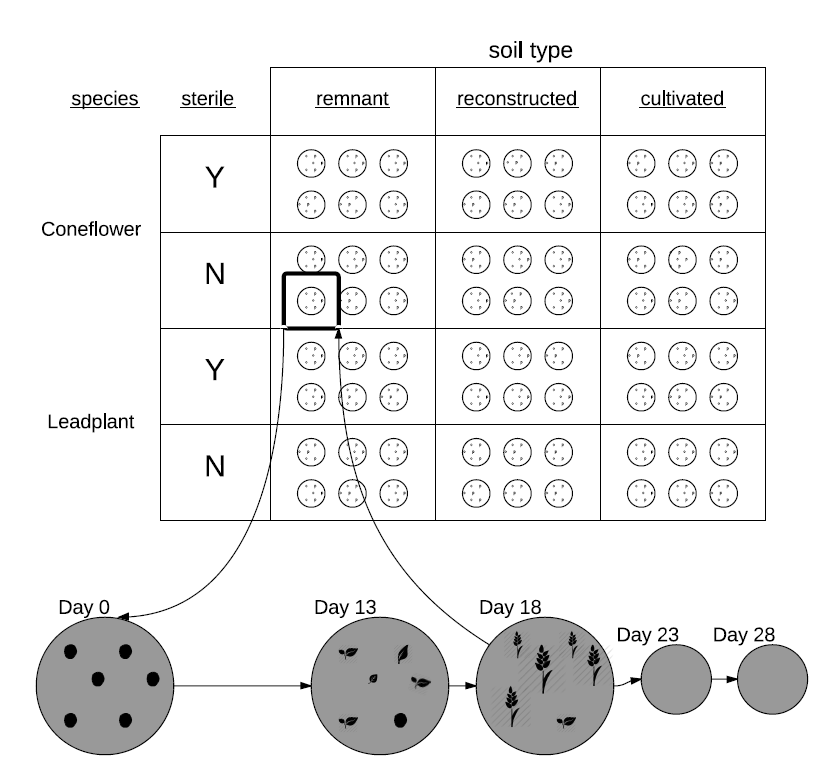
\includegraphics[width=0.8\linewidth]{data/StudyDesignDiagram} \caption{The design of the seed germination study}\label{fig:seedstudy}
\end{figure}

\hypertarget{explore3}{%
\section{Initial Exploratory Analyses}\label{explore3}}

\hypertarget{organizedata3}{%
\subsection{Data Organization}\label{organizedata3}}

Data for Case Study \ref{cs:seeds} in \texttt{seeds2.csv} contains the following variables:

\begin{itemize}
\tightlist
\item
  \texttt{pot} = Pot plant was grown in (1-72)
\item
  \texttt{plant} = Unique plant identification number
\item
  \texttt{species} = L for leadplant and C for coneflower
\item
  \texttt{soil} = STP for reconstructed prairie, REM for remnant prairie, and CULT for cultivated land
\item
  \texttt{sterile} = Y for yes and N for no
\item
  \texttt{germin} = Y if plant germinated, N if not
\item
  \texttt{hgt13} = height of plant (in mm) 13 days after seeds planted
\item
  \texttt{hgt18} = height of plant (in mm) 18 days after seeds planted
\item
  \texttt{hgt23} = height of plant (in mm) 23 days after seeds planted
\item
  \texttt{hgt28} = height of plant (in mm) 28 days after seeds planted
\end{itemize}

This data is stored in wide format, with one row per plant (see 12 sample plants in Table \ref{tab:table1chp10}). As we have done in previous multilevel analyses, we will convert to long format (one observation per plant-time combination) after examining the missing data pattern and removing any plants with no growth data. In this case, we are almost assuredly losing information by removing plants with no height data at all four time points, since these plants did not germinate, and there may well be differences between species, soil type, and sterilization with respect to germination rates. We will handle this possibility by analyzing germination rates separately (see Chapter \ref{ch-GLMM}); the analysis in this chapter will focus on effects of species, soil type, and sterilization on initial growth and growth rate among plants that germinate.

\begin{table}

\caption{\label{tab:table1chp10}A snapshot of data (Plants 231-246) from the Seed Germination case study in wide format.}
\centering
\resizebox{\linewidth}{!}{
\begin{tabular}[t]{lrrllllrrrr}
\toprule
  & pot & plant & soil & sterile & species & germin & hgt13 & hgt18 & hgt23 & hgt28\\
\midrule
135 & 23 & 231 & CULT & N & C & Y & 1.1 & 1.4 & 1.6 & 1.7\\
136 & 23 & 232 & CULT & N & C & Y & 1.3 & 2.2 & 2.5 & 2.7\\
137 & 23 & 233 & CULT & N & C & Y & 0.5 & 1.4 & 2.0 & 2.3\\
138 & 23 & 234 & CULT & N & C & Y & 0.3 & 0.4 & 1.2 & 1.7\\
139 & 23 & 235 & CULT & N & C & Y & 0.5 & 0.5 & 0.8 & 2.0\\
\addlinespace
140 & 23 & 236 & CULT & N & C & Y & 0.1 & NA & NA & NA\\
141 & 24 & 241 & STP & Y & L & Y & 1.8 & 2.6 & 3.9 & 4.2\\
142 & 24 & 242 & STP & Y & L & Y & 1.3 & 1.7 & 2.8 & 3.7\\
143 & 24 & 243 & STP & Y & L & Y & 1.5 & 1.6 & 3.9 & 3.9\\
144 & 24 & 244 & STP & Y & L & Y & NA & 1.0 & 2.3 & 3.8\\
\addlinespace
145 & 24 & 245 & STP & Y & L & N & NA & NA & NA & NA\\
146 & 24 & 246 & STP & Y & L & N & NA & NA & NA & NA\\
\bottomrule
\end{tabular}}
\end{table}

Although the experimental design called for \(72*6=432\) plants, the wide data set has 437 plants because a few pots had more than six plants (likely because two of the microscopically small seeds stuck together when planted). Of those 437 plants, 154 had no height data (did not germinate by the 28th day) and were removed from analysis (for example, see rows 145-146 in Table \ref{tab:table1chp10}). 248 plants had complete height data (e.g., rows 135-139 and 141-143), 13 germinated later than the 13th day but had complete heights once they germinated (e.g., row 144), and 22 germinated and had measurable height on the 13th day but died before the 28th day (e.g., row 140). Ultimately, the long data set contains 1132 unique observations where plants heights were recorded; representation of plants 236-242 in the long data set can be seen in Table \ref{tab:table2chp10}.

\begin{table}

\caption{\label{tab:table2chp10}A snapshot of data (Plants 236-242) from the Seed Germination case study in long format.}
\centering
\begin{tabular}[t]{rrllllrr}
\toprule
pot & plant & soil & sterile & species & germin & hgt & time13\\
\midrule
23 & 236 & CULT & N & C & Y & 0.1 & 0\\
23 & 236 & CULT & N & C & Y & NA & 5\\
23 & 236 & CULT & N & C & Y & NA & 10\\
23 & 236 & CULT & N & C & Y & NA & 15\\
24 & 241 & STP & Y & L & Y & 1.8 & 0\\
\addlinespace
24 & 241 & STP & Y & L & Y & 2.6 & 5\\
24 & 241 & STP & Y & L & Y & 3.9 & 10\\
24 & 241 & STP & Y & L & Y & 4.2 & 15\\
24 & 242 & STP & Y & L & Y & 1.3 & 0\\
24 & 242 & STP & Y & L & Y & 1.7 & 5\\
\addlinespace
24 & 242 & STP & Y & L & Y & 2.8 & 10\\
24 & 242 & STP & Y & L & Y & 3.7 & 15\\
\bottomrule
\end{tabular}
\end{table}

Notice the \textbf{three-level structure} \index{three-level structure} of this data. Treatments (levels of the three experimental factors) were assigned at the \texttt{pot} level, then multiple plants were grown in each pot, and multiple measurements were taken over time for each plant. Our multilevel analysis must therefore account for pot-to-pot variability in height measurements (which could result from factor effects), plant-to-plant variability in height within a single pot, and variability over time in height for individual plants. In order to fit such a three-level model, we must extend the two-level model which we have used thus far.

\hypertarget{explore3v2}{%
\subsection{Exploratory Analyses}\label{explore3v2}}

We start by taking an initial look at the effect of Level Three covariates (factors applied at the pot level: species, soil type, and sterilization) on plant height, pooling observations across pot, across plant, and across time of measurement within plant. First, we observe that the initial balance which existed after randomization of pot to treatment no longer holds. After removing plants that did not germinate (and therefore had no height data), more height measurements exist for coneflowers (n=704, compared to 428 for leadplants), soil from restored prairies (n=524, compared to 288 for cultivated land and 320 for remnant prairies), and unsterilized soil (n=612, compared to 520 for sterilized soil). This imbalance indicates possible factor effects on germination rate; we will take up those hypotheses in Chapter \ref{ch-GLMM}. In this chapter, we will focus on the effects of species, soil type, and sterilization on the growth patterns of plants that germinate.

Because we suspect that height measurements over time for a single plant are highly correlated, while height measurements from different plants from the same pot are less correlated, we calculate mean height per plant (over all available time points) before generating exploratory plots investigating Level Three factors. Figure \ref{fig:boxbyspec} then examines the effects of soil type and sterilization separately by species. Sterilization seems to have a bigger benefit for coneflowers, while soil from remnant prairies seems to lead to smaller leadplants and taller coneflowers.

\begin{figure}

{\centering 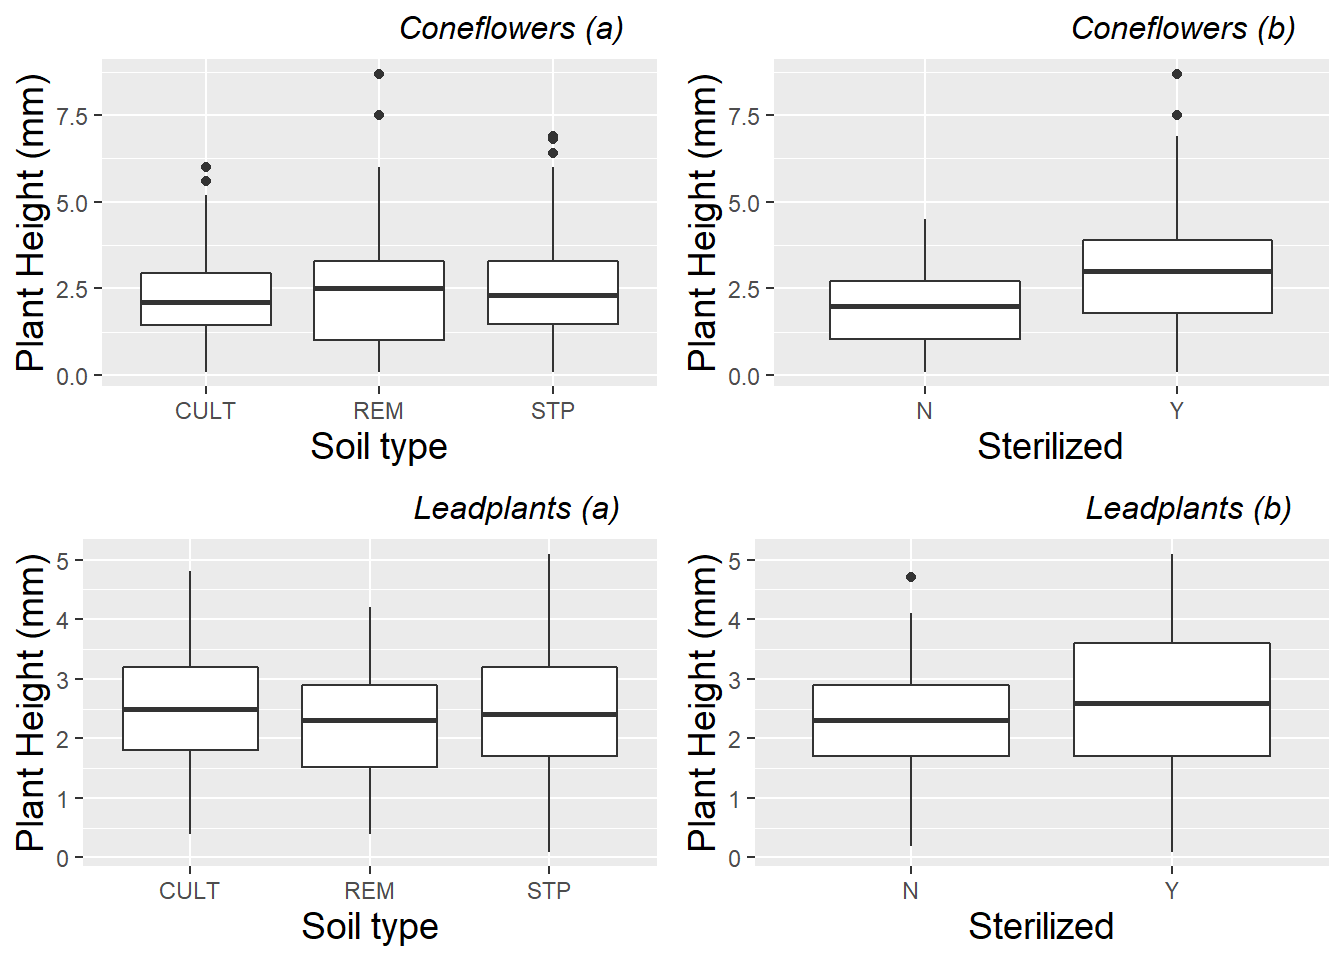
\includegraphics[width=0.6\linewidth]{bookdown-bysh_files/figure-latex/boxbyspec-1} 

}

\caption{Plant height comparisons of (a) soil type and (b) sterilization within species.  Each plant is represented by the mean height over all measurements at all time points for that plant.}\label{fig:boxbyspec}
\end{figure}

We also use spaghetti plots to examine time trends within species to see (a) if it is reasonable to assume linear growth between Day 13 and Day 28 after planting, and (b) if initial height and rate of growth is similar in the two species. Figure \ref{fig:spagbyspec} illustrates differences between species. While both species have similar average heights 13 days after planting, coneflowers appear to have faster early growth which slows later, while leadplants have a more linear growth rate which culminates in greater average heights 28 days after planting. Coneflowers also appear to have greater variability in initial height and growth rate, although there are more coneflowers with height data.

\begin{figure}

{\centering 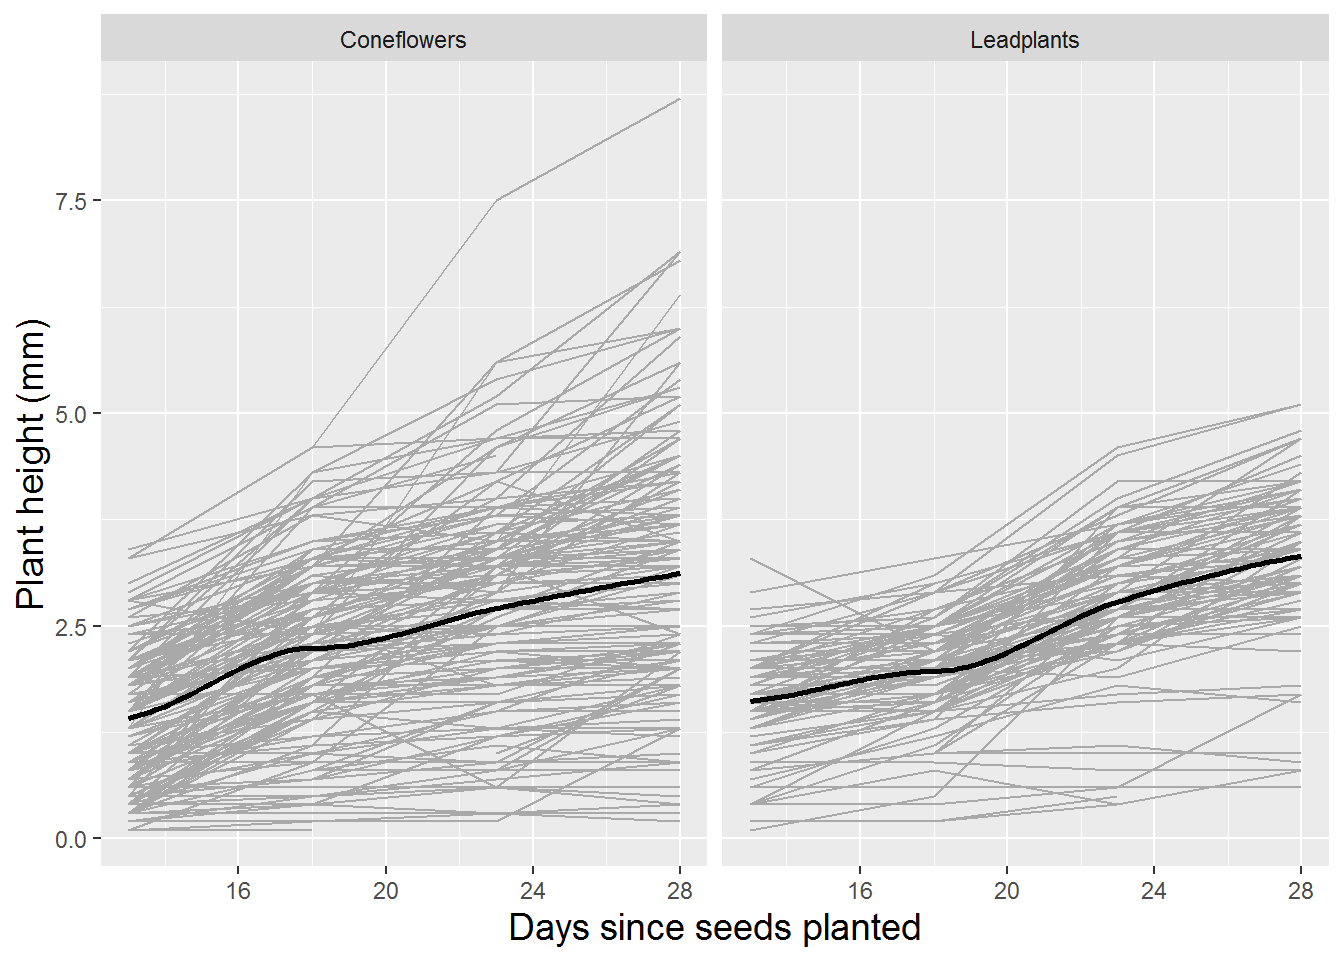
\includegraphics[width=0.6\linewidth]{bookdown-bysh_files/figure-latex/spagbyspec-1} 

}

\caption{Spaghetti plot by species with loess fit.  Each "line" represents one plant.}\label{fig:spagbyspec}
\end{figure}

Exploratory analyses such as these confirm the suspicions of biology researchers that leadplants and coneflowers should be analyzed separately. Because of biological differences, it is expected that these two species will show different growth patterns and respond differently to treatments such as fertilization. Coneflowers are members of the aster family, growing up to 4 feet tall with their distinctive gray seed heads and drooping yellow petals. Leadplants, on the other hand, are members of the bean family, with purple flowers, a height of 1 to 3 feet, and compound greyish green leaves which look to be dusted with white lead. Leadplants have deep root systems and are symbiotic N-fixers, which means they might experience stifled growth in sterilized soil compared with other species. For the remainder of this chapter, we will focus on \textbf{leadplants} and how their growth patterns are affected by soil type and sterilization. You will have a chance to analyze coneflower data later in the Exercises section.

Lattice plots, illustrating several observational units simultaneously, each with fitted lines where appropriate, are also valuable to examine during the exploratory analysis phase. Figure \ref{fig:lattlpall} shows height over time for 24 randomly selected leadplants that germinated in this study, with a fitted linear regression line. Linearity appears reasonable in most cases, although there is some variability in the intercepts and a good deal of variability in the slopes of the fitted lines. These intercepts and slopes by plant, of course, will be potential parameters in a multilevel model which we will fit to this data. Given the three-level nature of this data, it is also useful to examine a spaghetti plot by pot (Figure \ref{fig:spaglppot}). While linearity appears to reasonably model the average trend over time within pot, we see differences in the plant-to-plant variability within pot, but some consistency in intercept and slope from pot to pot.

\begin{figure}

{\centering 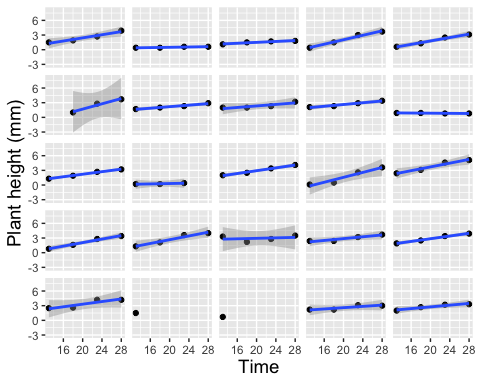
\includegraphics[width=0.6\linewidth]{bookdown-bysh_files/figure-latex/lattlpall-1} 

}

\caption{ Lattice plot of linear trends fit to 24 randomly selected leadplants.  One plant with only a single height measurement has no associated regression line.}\label{fig:lattlpall}
\end{figure}

\begin{figure}

{\centering 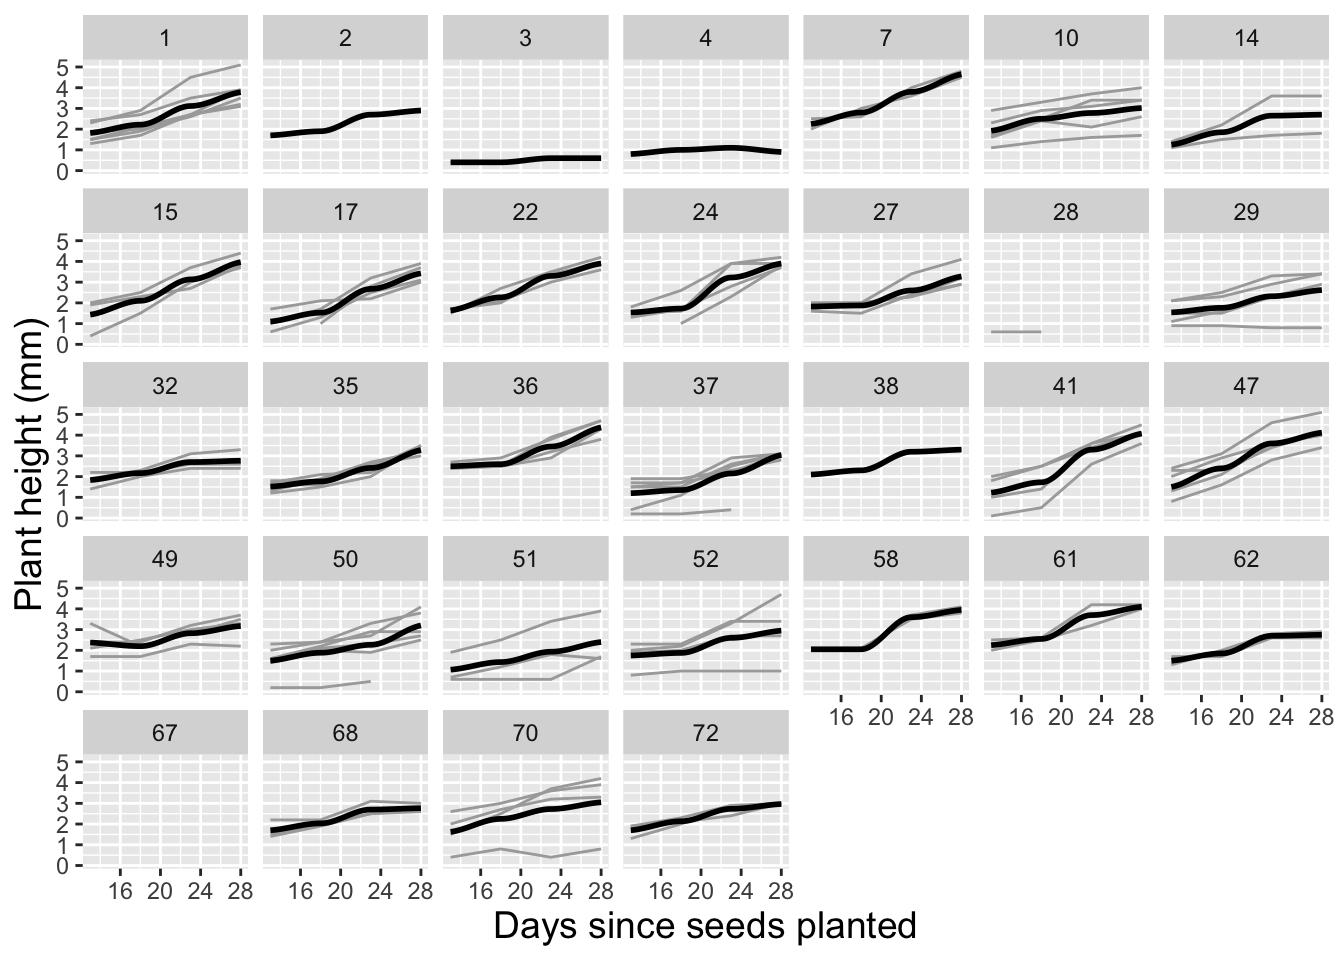
\includegraphics[width=0.6\linewidth]{bookdown-bysh_files/figure-latex/spaglppot-1} 

}

\caption{Spaghetti plot for leadplants by pot with loess fit.}\label{fig:spaglppot}
\end{figure}

Spaghetti plots can also be an effective tool for examining the potential effects of soil type and sterilization on growth patterns of leadplants. Figure \ref{fig:spaglpsoil} and Figure \ref{fig:spaglpster} illustrate how the growth patterns of leadplants depend on soil type and sterilization. In general, we observe slower growth in soil from remnant prairies and soil that has not been sterilized.

\begin{figure}

{\centering 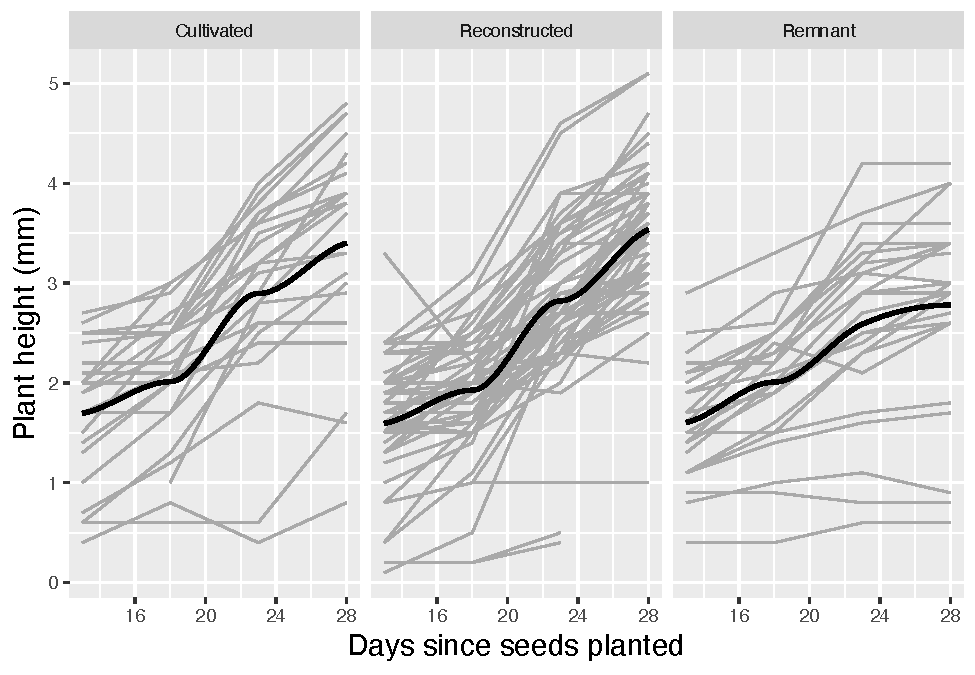
\includegraphics[width=0.6\linewidth]{bookdown-bysh_files/figure-latex/spaglpsoil-1} 

}

\caption{Spaghetti plot for leadplants by soil type with loess fit.}\label{fig:spaglpsoil}
\end{figure}

\begin{figure}

{\centering 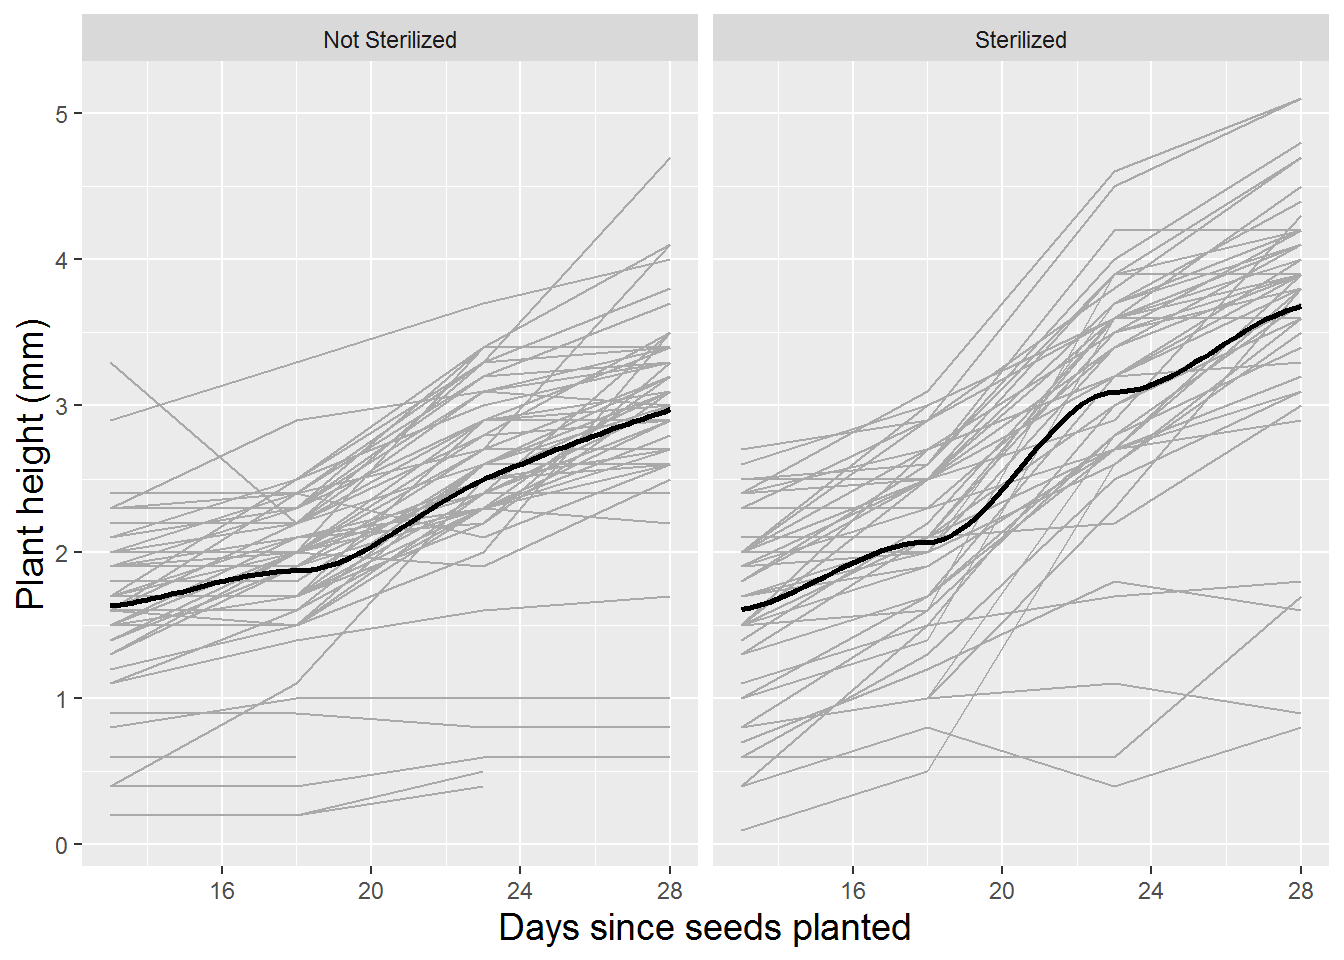
\includegraphics[width=0.6\linewidth]{bookdown-bysh_files/figure-latex/spaglpster-1} 

}

\caption{Spaghetti plot for leadplants by sterilization with loess fit.}\label{fig:spaglpster}
\end{figure}

We can further explore the variability in linear growth among plants and among pots by fitting regression lines and examining the estimated intercepts and slopes, as well as the corresponding \(R^2\) values. Figures \ref{fig:intrateplant} and \ref{fig:intratepot} provide just such an analysis, where Figure \ref{fig:intrateplant} shows results of fitting lines by plant, and Figure \ref{fig:intratepot} shows results of fitting lines by pot. Certain caveats accompany these summaries. In the case of fitted lines by plant, each plant is given equal weight regardless of the number of observations (2-4) for a given plant, and in the case of fitted lines by pot, a line is estimated by simply pooling all observations from a given pot, ignoring the plant from which the observations came, and equally weighting pots regardless of how many plants germinated and survived to Day 28. Nevertheless, the summaries of fitted lines provide useful information. When fitting regression lines by plant, we see a mean intercept of 1.52 (SD=0.66), indicating an estimated average height at 13 days of 1.5 mm, and a mean slope of 0.114 mm per day of growth from Days 13 to 28 (SD=0.059). Most R-squared values were strong (e.g., 84\% were above 0.8). Summaries of fitted regression lines by pot show similar mean intercepts (1.50) and slopes (0.107), but somewhat less variability pot-to-pot than we observed plant-to-plant (SD=0.46 for intercepts and SD=0.050 for slopes).

\begin{figure}

{\centering 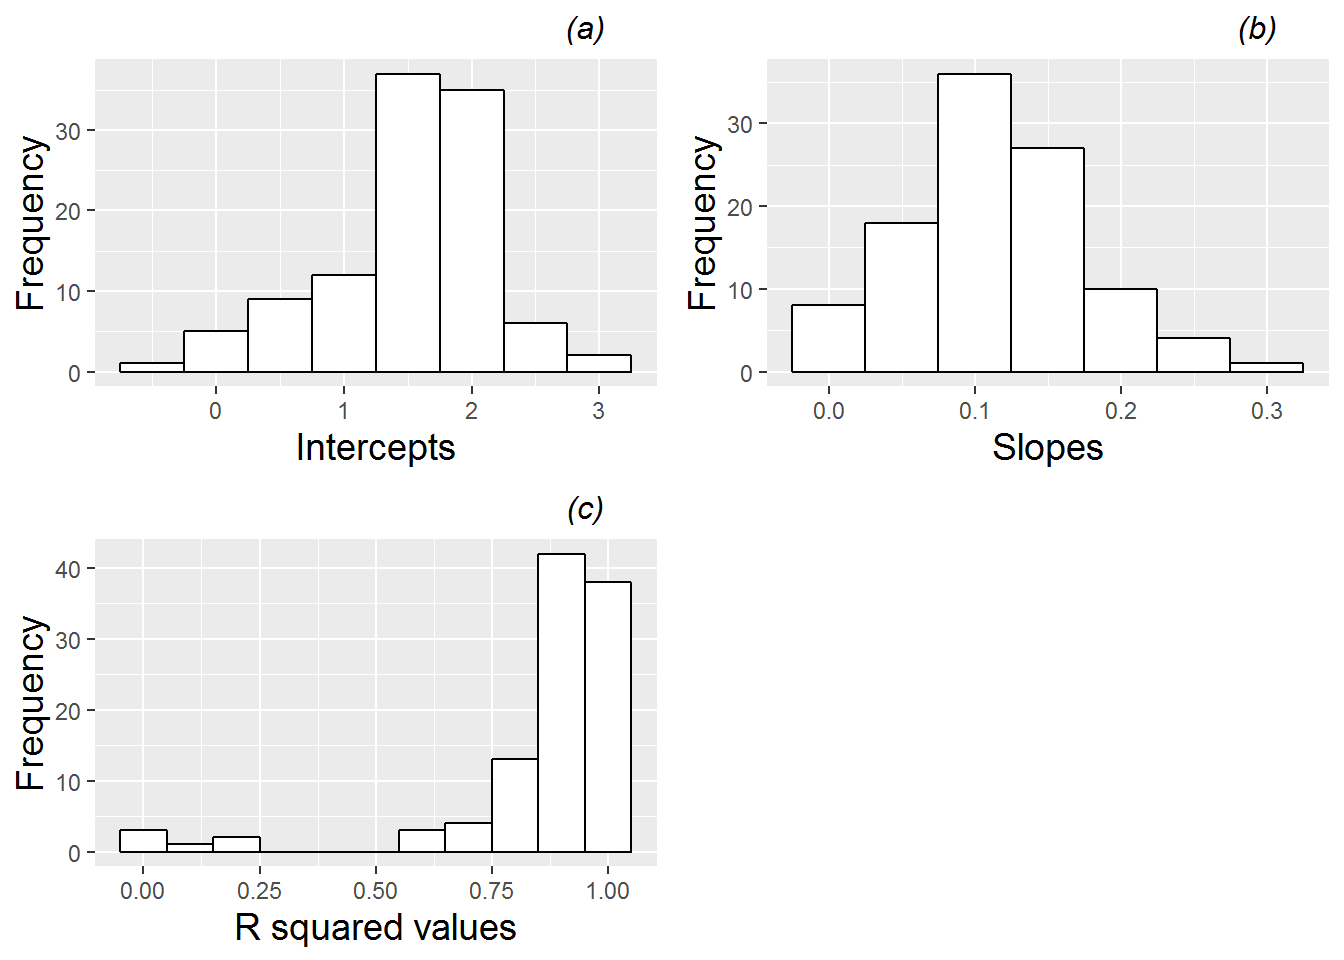
\includegraphics[width=0.6\linewidth]{bookdown-bysh_files/figure-latex/intrateplant-1} 

}

\caption{ Histograms of (a) intercepts, (b) slopes, and (c) R-squared values for linear fits across all leadplants.}\label{fig:intrateplant}
\end{figure}

\begin{figure}

{\centering 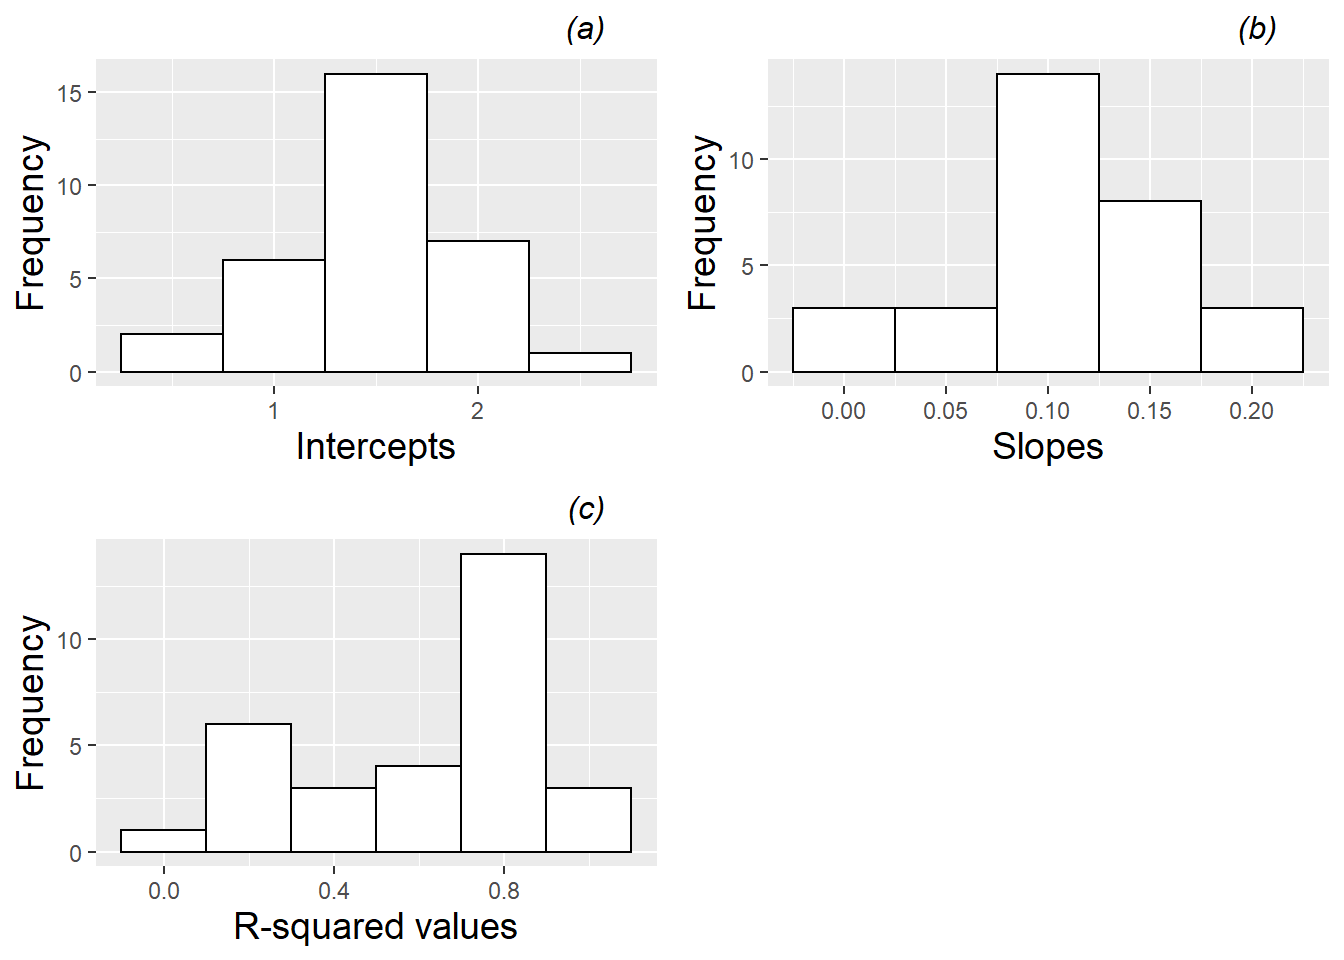
\includegraphics[width=0.6\linewidth]{bookdown-bysh_files/figure-latex/intratepot-1} 

}

\caption{Histograms of (a) intercepts, (b) slopes, and (c) R-squared values for linear fits across all pots with leadplants.}\label{fig:intratepot}
\end{figure}

Another way to examine variability due to plant vs.~variability due to pot is through summary statistics. Plant-to-plant variability can be estimated by averaging standard deviations from each pot (.489 for intercepts and .039 for slopes), while pot-to-pot variability can be estimated by finding the standard deviation of average intercept (.478) or slope (.051) within pot. Based on these rough measurements, variability due to plants and pots is comparable.

Fitted lines by plant and pot are modeled using a centered time variable (\texttt{time13}), adjusted so that the first day of height measurements (13 days after planting) corresponds to \texttt{time13}=0. This centering has two primary advantages. First, the estimated intercept becomes more interpretable. Rather than representing height on the day of planting (which should be 0 mm, but which represents a hefty extrapolation from our observed range of days 13 to 28), the intercept now represents height on Day 13. Second, the intercept and slope are much less correlated (r=-0.16) than when uncentered time is used, which improves the stability of future models.

Fitted intercepts and slopes by plant can be used for an additional exploratory examination of factor effects to complement those from the earlier spaghetti plots. Figure \ref{fig:irboxbyspec} complements Figure \ref{fig:spagbyspec}, again showing differences between species---coneflowers tend to start smaller and have slower growth rates, although they have much more variability in growth patterns than leadplants. Returning to our focus on leadplants, Figure \ref{fig:irboxbysoil} shows that plants grown in soil from cultivated fields tends to be taller at Day 13, and plants grown in soil from remnant prairies tend to grow more slowly than plants grown in other soil types. Figure \ref{fig:irboxbyster} shows the strong tendency for plants grown in sterilized soil to grow faster than plants grown in non-sterilized soil. We will soon see if our fitted multilevel models support these observed trends.

\begin{figure}

{\centering 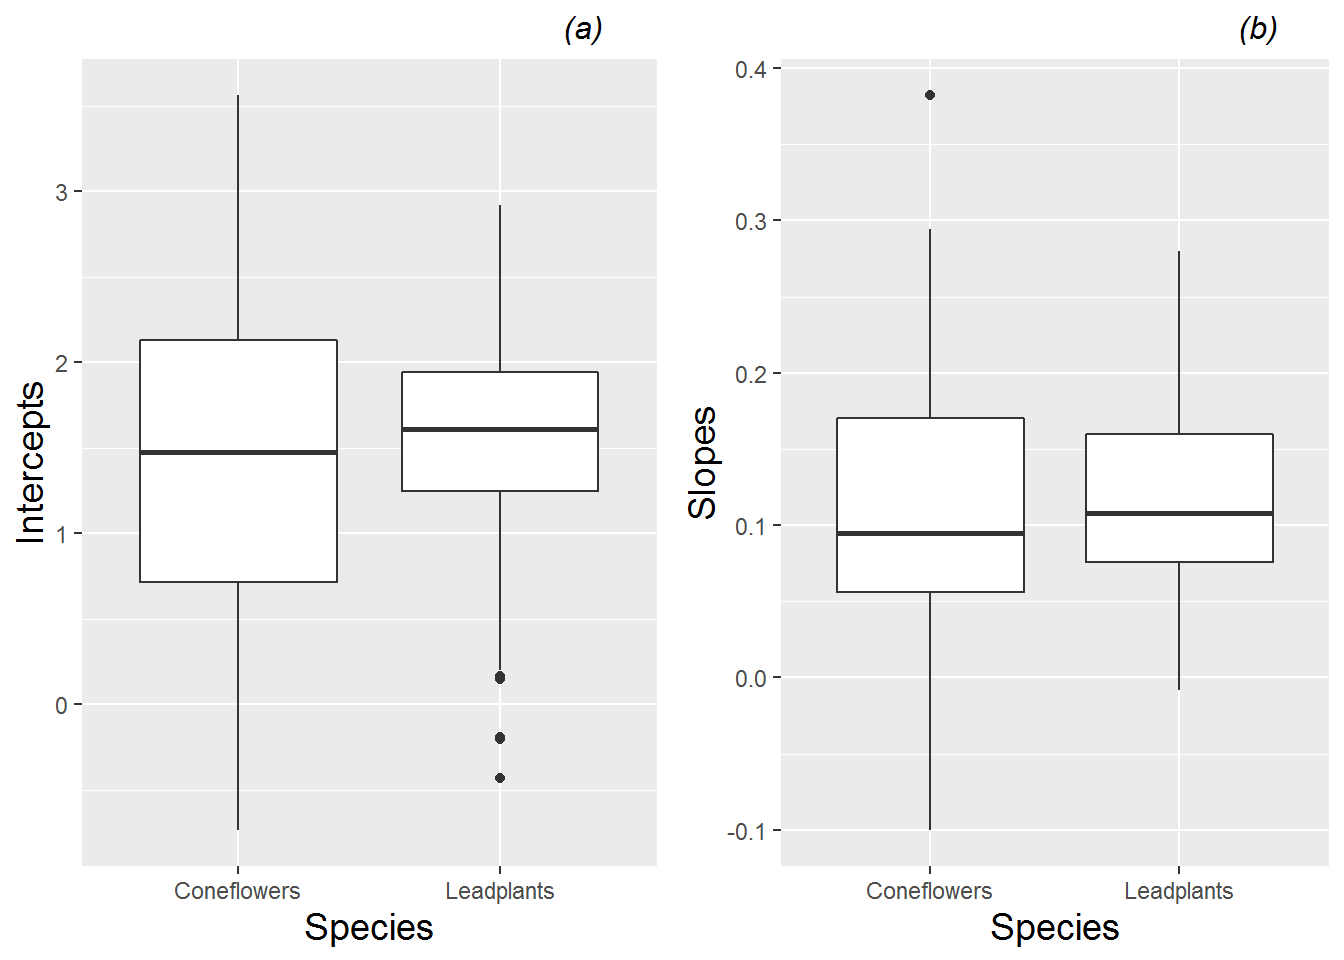
\includegraphics[width=0.6\linewidth]{bookdown-bysh_files/figure-latex/irboxbyspec-1} 

}

\caption{Boxplots of (a) intercepts and (b) slopes for all plants by species, based on a linear fit to height data from each plant.}\label{fig:irboxbyspec}
\end{figure}

\begin{figure}

{\centering 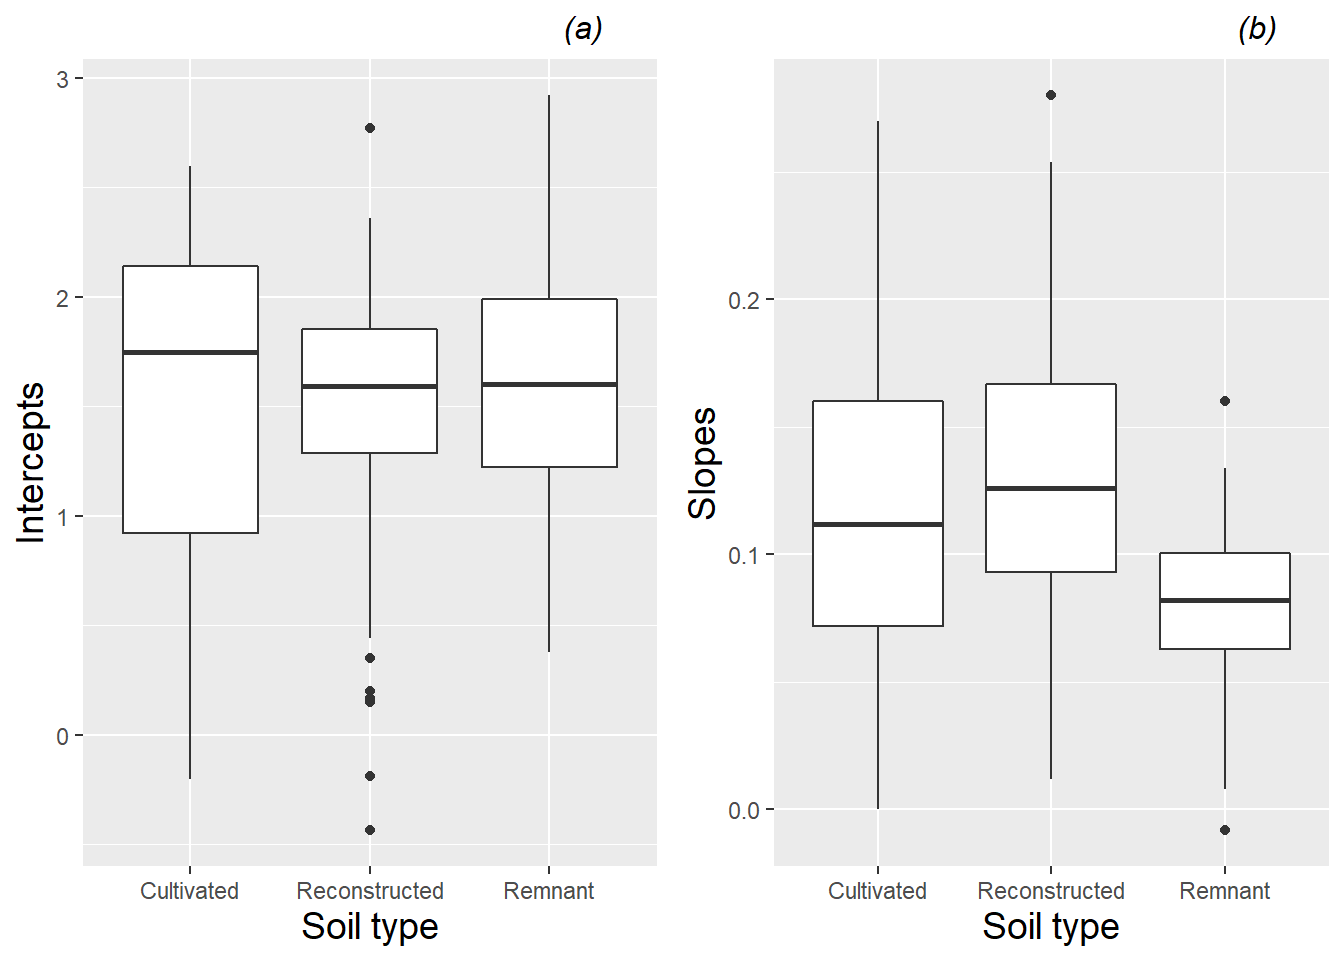
\includegraphics[width=0.6\linewidth]{bookdown-bysh_files/figure-latex/irboxbysoil-1} 

}

\caption{Boxplots of (a) intercepts and (b) slopes for all leadplants by soil type, based on a linear fit to height data from each plant.}\label{fig:irboxbysoil}
\end{figure}

\begin{figure}

{\centering 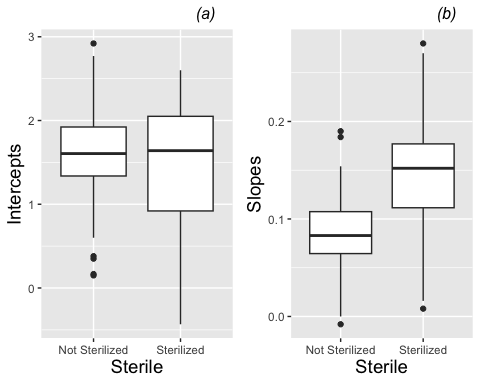
\includegraphics[width=0.6\linewidth]{bookdown-bysh_files/figure-latex/irboxbyster-1} 

}

\caption{Boxplots of (a) intercepts and (b) slopes for all leadplants by sterilization, based on a linear fit to height data from each plant.}\label{fig:irboxbyster}
\end{figure}

Since we have time at Level One, any exploratory analysis of Case Study \ref{cs:seeds} should contain an investigation of the variance-covariance structure within plant. Figure \ref{fig:corrstruct} shows the potential for an autocorrelation structure in which the correlation between observations from the same plant diminishes as the time between measurements increases. Residuals five days apart have correlations ranging from .77 to .91, while measurements ten days apart have correlations of .62 and .70, and measurements fifteen days apart have correlation of .58.

\begin{figure}

{\centering \includegraphics[width=0.6\linewidth]{bookdown-bysh_files/figure-latex/corrstruct-1} 

}

\caption{Correlation structure within plant.  The upper right contains correlation coefficients between residuals at pairs of time points, the lower left contains scatterplots of the residuals at time point pairs, and the diagonal contains histograms of residuals at each of the four time points.}\label{fig:corrstruct}
\end{figure}

\hypertarget{initialmodels-3level}{%
\section{Initial models: unconditional means and unconditional growth}\label{initialmodels-3level}}

The structure and notation for three level models will closely resemble the structure and notation for two level models, just with extra subscripts. Therein lies some of the power of multilevel models---extensions are relatively easy and allow you to control for many sources of variability, obtaining more precise estimates of important parameters. However, the number of variance component parameters to estimate can quickly mushroom as covariates are added at lower levels, so implementing simplifying restrictions will often become necessary (see Section \ref{sec:explodingvarcomps}).

We once again begin with the \textbf{unconditional means model} \index{unconditional means model}, in which there are no predictors at any level, in order to assess the amount of variation at each level. Here, Level Three is pot, Level Two is plant within pot, and Level One is time within plant. Using model formulations at each of the three levels, the unconditional means three-level model can be expressed as:

\begin{itemize}
\tightlist
\item
  Level One (timepoint within plant):
\end{itemize}

\begin{equation*}
Y_{ijk} = a_{ij}+\epsilon_{ijk} \textrm{ where } \epsilon_{ijk}\sim N(0,\sigma^2)
\end{equation*}

\begin{itemize}
\tightlist
\item
  Level Two (plant within pot):
\end{itemize}

\begin{equation*}
a_{ij} = a_{i}+u_{ij} \textrm{ where } u_{ij}\sim N(0,\sigma_{u}^{2})
\end{equation*}

\begin{itemize}
\tightlist
\item
  Level Three (pot):
\end{itemize}

\begin{equation*}
a_{i} = \alpha_{0}+\tilde{u}_{i} \textrm{ where } \tilde{u}_{i} \sim N(0,\sigma_{\tilde{u}}^{2})
\end{equation*}

where the heights of plants from different pots are considered independent, but plants from the same pot are correlated as well as measurements at different times from the same plant.

Keeping track of all the model terms, especially with three subscripts, is not a trivial task, but it's worth spending time thinking through. Here is a quick guide to the meaning of terms found in our three-level model:

\begin{itemize}
\tightlist
\item
  \(Y_{ijk}\) is the height (in mm) of plant \(j\) from pot \(i\) at time \(k\)
\item
  \(a_{ij}\) is the true mean height for plant \(j\) from pot \(i\) across all time points. This is not considered a model parameter, since we further model \(a_{ij}\) at Level Two.
\item
  \(a_{i}\) is the true mean height for pot \(i\) across all plants from that pot and all time points. This is also not considered a model parameter, since we further model \(a_{i}\) at Level Three.
\item
  \(\alpha_{0}\) is a fixed effects model parameter representing the true mean height across all pots, plants, and time points
\item
  \(\epsilon_{ijk}\) describes how far an observed height \(Y_{ijk}\) is from the mean height for plant \(j\) from pot \(i\)
\item
  \(u_{ij}\) describe how far the mean height of plant \(j\) from pot \(i\) is from the mean height of all plants from pot \(i\)
\item
  \(\tilde{u}_{i}\) describes how far the mean height of all observations from pot \(i\) is from the overall mean height across all pots, plants, and time points. None of the error terms (\(\epsilon, u, \tilde{u}\)) are considered model parameters; they simply account for differences between the observed data and expected values under our model.
\item
  \(\sigma^2\) is a variance component (random effects model parameter) that describes within-plant variability over time
\item
  \(\sigma_{u}^{2}\) is the variance component describing plant-to-plant variability within pot
\item
  \(\sigma_{\tilde{u}}^{2}\) is the variance component describing pot-to-pot variability.
\end{itemize}

The three-level unconditional means model can also be expressed as a composite model:

\begin{equation*}
Y_{ijk}=\alpha_{0}+\tilde{u}_{i}+u_{ij}+\epsilon_{ijk}
\end{equation*}
and this composite model can be fit using statistical software:

\begin{Shaded}
\begin{Highlighting}[]
\CommentTok{# Model A - unconditional means}
\NormalTok{modelal =}\StringTok{ }\KeywordTok{lmer}\NormalTok{(hgt }\OperatorTok{~}\StringTok{ }\DecValTok{1} \OperatorTok{+}\StringTok{ }\NormalTok{(}\DecValTok{1}\OperatorTok{|}\NormalTok{plant) }\OperatorTok{+}\StringTok{ }\NormalTok{(}\DecValTok{1}\OperatorTok{|}\NormalTok{pot), }
               \DataTypeTok{REML=}\NormalTok{T, }\DataTypeTok{data=}\NormalTok{leaddata)}
\end{Highlighting}
\end{Shaded}

\begin{verbatim}
##  Groups   Name        Variance Std.Dev.
##  plant    (Intercept) 0.2782   0.527   
##  pot      (Intercept) 0.0487   0.221   
##  Residual             0.7278   0.853
\end{verbatim}

\begin{verbatim}
##  Number of Level Two groups =  107 
##  Number of Level Three groups =  32
\end{verbatim}

\begin{verbatim}
##             Estimate Std. Error t value
## (Intercept)    2.388    0.07887   30.28
\end{verbatim}

From this output, we obtain estimates of our four model parameters:

\begin{itemize}
\tightlist
\item
  \(\hat{\alpha}_{0}=2.39=\) the mean height (in mm) across all time points, plants, and pots.
\item
  \(\hat{\sigma}^2=0.728=\) the variance over time within plants.
\item
  \(\hat{\sigma}_{u}^{2}=0.278=\) the variance between plants from the same pot.
\item
  \(\hat{\sigma}_{\tilde{u}}^{2}=0.049=\) the variance between pots.
\end{itemize}

From the estimates of variance components, 69.0\% of total variability in height measurements is due to differences over time for each plant, 26.4\% of total variability is due to differences between plants from the same pot, and only 4.6\% of total variability is due to difference between pots. Accordingly, we will next explore whether the incorporation of time as a linear predictor at Level One can reduce the unexplained variability within plant.

The \textbf{unconditional growth model} \index{unconditional growth model} introduces time as a predictor at Level One, but there are still no predictors at Levels Two or Three. The unconditional growth model allows us to assess how much of the within-plant variability (the variability among height measurements from the same plant at different time points) can be attributed to linear changes over time, while also determining how much variability we see in the intercept (Day 13 height) and slope (daily growth rate) from plant-to-plant and pot-to-pot. Later, we can model plant-to-plant and pot-to-pot differences in intercepts and slopes with Level Two and Three covariates.

The three-level unconditional growth model (Model B) can be specified either using formulations at each level:

\begin{itemize}
\tightlist
\item
  Level One (timepoint within plant):
\end{itemize}

\begin{equation*}
Y_{ijk} = a_{ij}+b_{ij}\textrm{time}_{ijk}+\epsilon_{ijk}
\end{equation*}

\begin{itemize}
\tightlist
\item
  Level Two (plant within pot):
\end{itemize}

\begin{align*}
a_{ij} & = a_{i}+u_{ij} \\
b_{ij} & = b_{i}+v_{ij}
\end{align*}

\begin{itemize}
\tightlist
\item
  Level Three (pot):
\end{itemize}

\begin{align*}
a_{i} & = \alpha_{0}+\tilde{u}_{i} \\
b_{i} & = \beta_{0}+\tilde{v}_{i}
\end{align*}

or as a composite model:

\begin{equation*}
Y_{ijk}=[\alpha_{0}+\beta_{0}\textrm{time}_{ijk}]+
[\tilde{u}_{i}+{v}_{ij}+\epsilon_{ijk}+(\tilde{v}_{i}+{v}_{ij})\textrm{time}_{ijk}]
\end{equation*}

where \(\epsilon_{ijk}\sim N(0,\sigma^2)\),

\[ \left[ \begin{array}{c}
            u_{ij} \\ v_{ij}
          \end{array}  \right] \sim N \left( \left[
          \begin{array}{c}
            0 \\ 0
          \end{array} \right], \left[
          \begin{array}{cc}
            \sigma_{u}^{2} & \\
            \sigma_{uv} & \sigma_{v}^{2}
          \end{array} \right] \right), \] and

\[ \left[ \begin{array}{c}
            \tilde{u}_{i} \\ \tilde{v}_{i}
          \end{array}  \right] \sim N \left( \left[
          \begin{array}{c}
            0 \\ 0
          \end{array} \right], \left[
          \begin{array}{cc}
            \sigma_{\tilde{u}}^{2} & \\
            \sigma_{\tilde{u}\tilde{v}} & \sigma_{\tilde{v}}^{2}
          \end{array} \right] \right). \]

In this model, at Level One the trajectory for plant \(j\) from pot \(i\) is assumed to be linear, with intercept \(a_{ij}\) (height on Day 13) and slope \(b_{ij}\) (daily growth rate between Days 13 and 28); the \(\epsilon_{ijk}\) terms capture the deviation between the true growth trajectory of plant \(j\) from pot \(i\) and its observed heights. At Level Two, \(a_{i}\) represents the true mean intercept and \(b_{i}\) represents the true mean slope for all plants from pot \(i\), while \(u_{ij}\) and \(v_{ij}\) capture the deviation between plant \(j\)'s true growth trajectory and the mean intercept and slope for pot \(i\). The deviations in intercept and slope at Level Two are allowed to be correlated through the covariance parameter \(\sigma_{uv}\). Finally, \(\alpha_{0}\) is the true mean intercept and \(\beta_{0}\) is the true mean daily growth rate over the entire population of leadplants, while \(\tilde{u}_{i}\) and \(\tilde{v}_{i}\) capture the deviation between pot \(i\)'s true overall growth trajectory and the population mean intercept and slope. Note that between-plant and between-pot variability are both partitioned now into variability in initial status (\(\sigma_{u}^{2}\) and \(\sigma_{\tilde{u}}^{2}\)) and variability in rates of change (\(\sigma_{v}^{2}\) and \(\sigma_{\tilde{v}}^{2}\)).

Using the composite model specification, the unconditional growth model can be fit to the seed germination data:

\begin{Shaded}
\begin{Highlighting}[]
\CommentTok{# Model B - unconditional growth}
\NormalTok{modelbl =}\StringTok{ }\KeywordTok{lmer}\NormalTok{(hgt }\OperatorTok{~}\StringTok{ }\NormalTok{time13 }\OperatorTok{+}\StringTok{ }\NormalTok{(time13}\OperatorTok{|}\NormalTok{plant) }\OperatorTok{+}\StringTok{ }\NormalTok{(time13}\OperatorTok{|}\NormalTok{pot),}
               \DataTypeTok{REML=}\NormalTok{T, }\DataTypeTok{data=}\NormalTok{leaddata)}
\end{Highlighting}
\end{Shaded}

\begin{verbatim}
##  Groups   Name        Variance Std.Dev. Corr 
##  plant    (Intercept) 0.29914  0.5469        
##           time13      0.00119  0.0346   0.28 
##  pot      (Intercept) 0.04423  0.2103        
##           time13      0.00126  0.0355   -0.61
##  Residual             0.08216  0.2866
\end{verbatim}

\begin{verbatim}
##  Number of Level Two groups =  107 
##  Number of Level Three groups =  32
\end{verbatim}

\begin{verbatim}
##             Estimate Std. Error t value
## (Intercept)   1.5377   0.070305   21.87
## time13        0.1121   0.007924   14.15
\end{verbatim}

From this output, we obtain estimates of our nine model parameters (two fixed effects and seven variance components):

\begin{itemize}
\tightlist
\item
  \(\hat{\alpha}_{0}=1.538=\) the mean height of leadplants 13 days after planting.
\item
  \(\hat{\beta}_{0}=0.112=\) the mean daily change in height of leadplants from 13 to 28 days after planting.
\item
  \(\hat{\sigma}=.287=\) the standard deviation in within-plant residuals after accounting for time.
\item
  \(\hat{\sigma}_{u}=.547=\) the standard deviation in Day 13 heights between plants from the same pot.
\item
  \(\hat{\sigma}_{v}=.0346=\) the standard deviation in rates of change in height between plants from the same pot.
\item
  \(\hat{\rho}_{uv}=.280=\) the correlation in plants' Day 13 height and their rate of change in height.
\item
  \(\hat{\sigma}_{\tilde{u}}=.210=\) the standard deviation in Day 13 heights between pots.
\item
  \(\hat{\sigma}_{\tilde{v}}=.0355=\) the standard deviation in rates of change in height between pots.
\item
  \(\hat{\rho}_{\tilde{u}\tilde{v}}=-.610=\) the correlation in pots' Day 13 height and their rate of change in height.
\end{itemize}

We see that, on average, leadplants have a height of 1.54 mm thirteen days after planting (pooled across pots and treatment groups), and their heights tend to grow by 0.11 mm per day, producing an average height at the end of the study (Day 28) of 3.22 mm. According to the t-values listed in R, both the Day 13 height and the growth rate are statistically significant. The estimated within-plant variance \(\hat{\sigma}^2\) decreased by 88.7\% from the unconditional means model (from 0.728 to 0.082), implying that 88.7\% of within-plant variability in height can be explained by linear growth over time.

\hypertarget{sec:boundary}{%
\section{Encountering boundary constraints}\label{sec:boundary}}

Typically, with models consisting of three or more levels, the next step after adding covariates at Level One (such as time) is considering covariates at Level Two. In the seed germination experiment, however, there are no Level Two covariates of interest, and the treatments being studied were applied to pots (Level Three). We are primarily interested in the effects of soil type and sterilization on the growth of leadplants. Since soil type is a categorical factor with three levels, we can represent soil type in our model with indicator variables for cultivated lands (\texttt{cult}) and remnant prairies (\texttt{rem}), using reconstructed prairies as the reference level. For sterilization, we create a single indicator variable (\texttt{strl}) which takes on the value 1 for sterilized soil.

Our Level One and Level Two models will look identical to those from Model B; our Level Three models will contain the new covariates for soil type (\texttt{cult} and \texttt{rem}) and sterilization (\texttt{strl}):

\begin{align*}
a_{i} & = \alpha_{0}+\alpha_{1}\textrm{strl}_{i}+\alpha_{2}\textrm{cult}_{i}+\alpha_{3}\textrm{rem}_{i}+\tilde{u}_{i} \\
b_{i} & = \beta_{0}+\beta_{1}\textrm{strl}_{i}+\beta_{2}\textrm{cult}_{i}+\beta_{3}\textrm{rem}_{i}+\tilde{v}_{i}
\end{align*}

where the error terms at Level Three follow the same multivariate normal distribution as in Model B. In our case, the composite model can be written as:

\begin{align*}
Y_{ijk} & = (\alpha_{0}+\alpha_{1}\textrm{strl}_{i}+\alpha_{2}\textrm{cult}_{i}+\alpha_{3}\textrm{rem}_{i}+\tilde{u}_{i}+u_{ij}) + \\
 & (\beta_{0}+\beta_{1}\textrm{strl}_{i}+\beta_{2}\textrm{cult}_{i}+\beta_{3}\textrm{rem}_{i}+\tilde{v}_{i}+
 v_{ij})\textrm{time}_{ijk}+\epsilon_{ijk} 
\end{align*}

which, after combining fixed effects and random effects, can be rewritten as:

\begin{align*}
Y_{ijk} & = [\alpha_{0}+\alpha_{1}\textrm{strl}_{i}+\alpha_{2}\textrm{cult}_{i}+\alpha_{3}\textrm{rem}_{i} +
 \beta_{0}\textrm{time}_{ijk} + \\
 & \beta_{1}\textrm{strl}_{i}\textrm{time}_{ijk}+\beta_{2}\textrm{cult}_{i}\textrm{time}_{ijk}+ \beta_{3}\textrm{rem}_{i}\textrm{time}_{ijk}] + \\
 & [\tilde{u}_{i}+u_{ij}+\epsilon_{ijk}+\tilde{v}_{i}\textrm{time}_{ijk}+v_{ij}\textrm{time}_{ijk}]
\end{align*}

From the output below, the addition of Level Three covariates in Model C (\texttt{cult}, \texttt{rem}, \texttt{strl}, and their interactions with \texttt{time}) appears to provide a significant improvement (likelihood ratio test statistic = 32.2 on 6 df, \(p<.001\)) to the unconditional growth model (Model B).

\begin{Shaded}
\begin{Highlighting}[]
\CommentTok{# Model C - add covariates at pot level}
\NormalTok{modelcl =}\StringTok{ }\KeywordTok{lmer}\NormalTok{(hgt }\OperatorTok{~}\StringTok{ }\NormalTok{time13 }\OperatorTok{+}\StringTok{ }\NormalTok{strl }\OperatorTok{+}\StringTok{ }\NormalTok{cult }\OperatorTok{+}\StringTok{ }\NormalTok{rem }\OperatorTok{+}\StringTok{ }
\StringTok{    }\NormalTok{time13}\OperatorTok{:}\NormalTok{strl }\OperatorTok{+}\StringTok{ }\NormalTok{time13}\OperatorTok{:}\NormalTok{cult }\OperatorTok{+}\StringTok{ }\NormalTok{time13}\OperatorTok{:}\NormalTok{rem }\OperatorTok{+}\StringTok{ }\NormalTok{(time13}\OperatorTok{|}\NormalTok{plant) }\OperatorTok{+}
\StringTok{    }\NormalTok{(time13}\OperatorTok{|}\NormalTok{pot), }\DataTypeTok{REML=}\NormalTok{T, }\DataTypeTok{data=}\NormalTok{leaddata)}
\end{Highlighting}
\end{Shaded}

\begin{verbatim}
##  Groups   Name        Variance Std.Dev. Corr 
##  plant    (Intercept) 0.298087 0.5460        
##           time13      0.001208 0.0348   0.28 
##  pot      (Intercept) 0.053118 0.2305        
##           time13      0.000132 0.0115   -1.00
##  Residual             0.082073 0.2865
\end{verbatim}

\begin{verbatim}
##  Number of Level Two groups =  107 
##  Number of Level Three groups =  32
\end{verbatim}

\begin{verbatim}
##             Estimate Std. Error t value
## (Intercept)  1.50289   0.126992 11.8345
## time13       0.10107   0.008292 12.1889
## strl        -0.07655   0.151361 -0.5058
## cult         0.13002   0.182715  0.7116
## rem          0.13840   0.176189  0.7855
## time13:strl  0.05892   0.010282  5.7300
## time13:cult -0.02977   0.012263 -2.4273
## time13:rem  -0.03586   0.011978 -2.9939
\end{verbatim}

\begin{Shaded}
\begin{Highlighting}[]
\NormalTok{drop_in_dev <-}\StringTok{ }\KeywordTok{anova}\NormalTok{(modelbl, modelcl, }\DataTypeTok{test =} \StringTok{"Chisq"}\NormalTok{)}
\end{Highlighting}
\end{Shaded}

\begin{verbatim}
        npar   AIC   BIC logLik   dev Chisq Df
modelbl    9 603.8 640.0 -292.9 585.8    NA NA
modelcl   15 583.6 643.9 -276.8 553.6  32.2  6
             pval
modelbl        NA
modelcl 1.493e-05
\end{verbatim}

However, Model C has encountered a \textbf{boundary constraint} \index{boundary constraint} with an estimated Level 3 correlation between the intercept and slope error terms of -1. ``Allowable'' values of correlation coefficients run from -1 to 1; by definition, it is impossible to have a correlation between two error terms below -1. Thus, our estimate of -1 is right on the boundary of the allowable values. But how did this happen, and why is it potentially problematic?

Consider a model in which we have two parameters that must be estimated: \(\beta_0\) and \(\sigma^2\). As the intercept, \(\beta_0\) can take on any value; any real number is ``allowable''. But, by definition, variance terms such as \(\sigma^2\) must be non-negative; that is, \(\sigma^2 \geq 0\). Under the Principle of Maximum Likelihood, maximum likelihood estimators for \(\beta_0\) and \(\sigma^2\) will be chosen to maximize the likelihood of observing our given data. The left plot in Figure \ref{fig:boundary} shows hypothetical contours of the likelihood function \(L(\beta_0, \sigma^2)\); the likelihood is clearly maximized at \((\hat{\beta}_0 , \hat{\sigma}^2)=(4,-2)\). However, variance terms cannot be negative! A more sensible approach would have been to perform a constrained search for MLEs, considering any potential values for \(\beta_0\) but only non-negative values for \(\sigma^2\). This constrained search is illustrated in the right plot in Figure \ref{fig:boundary}. In this case, the likelihood is maximized at \((\hat{\beta}_0 , \hat{\sigma}^2)=(4,0)\). Note that the estimated intercept did not change, but the estimated variance is simply set at the smallest allowable value -- at the \textbf{boundary constraint}.



\begin{figure}

{\centering \includegraphics[width=0.6\linewidth]{bookdown-bysh_files/figure-latex/boundary-1} 

}

\caption{Left (a): hypothetical contours of the likelihood function \(L(\beta_0, \sigma^2)\) with no restrictions on \(\sigma^2\); the likelihood function is maximized at \((\hat{\beta}_0, \hat{\sigma}^2)=(4,-2)\). Right (b): hypothetical contours of the likelihood function \(L(\beta_0, \sigma^2)\) with the restriction that \(\sigma^2 \geq 0\); the constrained likelihood function is maximized at \((\hat{\beta}_0, \hat{\sigma}^2)=(4,0)\)}\label{fig:boundary}
\end{figure}

Graphically, in this simple illustration, the effect of the boundary constraint is to alter the likelihood function from a nice hill (in the left plot in Figure \ref{fig:boundary}) with a single peak at \((4,-2)\), to a hill with a huge cliff face where \(\sigma^2=0\). The highest point overlooking this cliff is at \((4,0)\), straight down the hill from the original peak.

In general, then, boundary constraints occur when the maximum likelihood estimator of at least one model parameter occurs at the limits of allowable values (such as estimated correlation coefficients of -1 or 1, or estimated variances of 0). Maximum likelihood estimates at the boundary tend to indicate that the likelihood function would be maximized at non-allowable values of that parameter, if an unconstrained search for MLEs was conducted. Most software packages, however, will only report maximum likelihood estimates with allowable values. Therefore, boundary constraints would ideally be avoided, if possible.

What should you do if you encounter boundary constraints? Often, boundary constraints signal that your model needs to be reparameterized -- i.e., you should alter your model to feature different parameters or ones that are interpreted differently. This can be accomplished in several ways:

\begin{itemize}
\tightlist
\item
  remove parameters, especially those variance and correlation terms which are being estimated on their boundaries
\item
  fix the values of certain parameters; for instance, you could set two variance terms equal to each other, thereby reducing the number of unknown parameters to estimate by one
\item
  transform covariates. Centering variables, standardizing variables, or changing units can all help stabilize a model. Numerical procedures for searching for and finding maximum likelihood estimates can encounter difficulties when variables have very high or low values, extreme ranges, outliers, or are highly correlated.
\end{itemize}

Although it is worthwhile attempting to reparameterize models to remove boundary constraints, sometimes they can be tolerated if (a) you are not interested in estimates of those parameters encountering boundary issues, and (b) removing those parameters does not affect conclusions about parameters of interest. For example, in the output below we explore the implications of simply removing the correlation between error terms at the pot level (i.e., assume \(\rho_{\tilde{u}\tilde{v}}=0\) rather than accepting the (constrained) maximum likelihood estimate of \(\hat{\rho}_{\tilde{u}\tilde{v}}=-1\) that we saw in Model C).

\begin{Shaded}
\begin{Highlighting}[]
\CommentTok{# Try Model C without correlation between L2 errors}
\NormalTok{modelcl.noL2corr <-}\StringTok{ }\KeywordTok{lmer}\NormalTok{(hgt }\OperatorTok{~}\StringTok{ }\NormalTok{time13 }\OperatorTok{+}\StringTok{ }\NormalTok{strl }\OperatorTok{+}\StringTok{ }\NormalTok{cult }\OperatorTok{+}\StringTok{ }\NormalTok{rem }\OperatorTok{+}
\StringTok{    }\NormalTok{time13}\OperatorTok{:}\NormalTok{strl }\OperatorTok{+}\StringTok{ }\NormalTok{time13}\OperatorTok{:}\NormalTok{cult }\OperatorTok{+}\StringTok{ }\NormalTok{time13}\OperatorTok{:}\NormalTok{rem }\OperatorTok{+}\StringTok{ }\NormalTok{(time13}\OperatorTok{|}\NormalTok{plant) }\OperatorTok{+}
\StringTok{    }\NormalTok{(}\DecValTok{1}\OperatorTok{|}\NormalTok{pot) }\OperatorTok{+}\StringTok{ }\NormalTok{(}\DecValTok{0}\OperatorTok{+}\NormalTok{time13}\OperatorTok{|}\NormalTok{pot), }\DataTypeTok{REML=}\NormalTok{T, }\DataTypeTok{data=}\NormalTok{leaddata)}
\end{Highlighting}
\end{Shaded}

\begin{verbatim}
##  Groups   Name        Variance Std.Dev. Corr
##  plant    (Intercept) 0.294076 0.5423       
##           time13      0.001206 0.0347   0.22
##  pot      (Intercept) 0.059273 0.2435       
##  pot.1    time13      0.000138 0.0117       
##  Residual             0.082170 0.2867
\end{verbatim}

\begin{verbatim}
##  Number of Level Two groups =  107 
##  Number of Level Three groups =  32
\end{verbatim}

\begin{verbatim}
##             Estimate Std. Error t value
## (Intercept)  1.51209   0.129695 11.6588
## time13       0.10158   0.008361 12.1490
## strl        -0.08742   0.154113 -0.5673
## cult         0.13233   0.185687  0.7126
## rem          0.10657   0.179363  0.5942
## time13:strl  0.05869   0.010382  5.6529
## time13:cult -0.03065   0.012337 -2.4843
## time13:rem  -0.03810   0.012096 -3.1500
\end{verbatim}

Note that the estimated variance components are all very similar to Model C, and the estimated fixed effects and their associated t-statistics are also very similar to Model C. Therefore, in this case we could consider simply reporting the results of Model C despite the boundary constraint.

However, when it is possible to remove boundary constraints through reasonable model reparameterizations, that is typically the preferred route. In this case, one option we might consider is simplifying Model C by setting \(\sigma_{\tilde{v}}^{2}=\sigma_{\tilde{u}\tilde{v}}=0\). We can then write our new model (Model C.1) in level-by-level formulation:

\begin{itemize}
\tightlist
\item
  Level One (timepoint within plant):
\end{itemize}

\begin{equation*}
Y_{ijk} = a_{ij}+b_{ij}\textrm{time}_{ijk}+\epsilon_{ijk}
\end{equation*}

\begin{itemize}
\tightlist
\item
  Level Two (plant within pot):
\end{itemize}

\begin{align*}
a_{ij} & = a_{i}+u_{ij} \\
b_{ij} & = b_{i}+v_{ij}
\end{align*}

\begin{itemize}
\tightlist
\item
  Level Three (pot):
\end{itemize}

\begin{align*}
a_{i} & = \alpha_{0}+\alpha_{1}\textrm{strl}_{i}+\alpha_{2}\textrm{cult}_{i}+\alpha_{3}\textrm{rem}_{i}+\tilde{u}_{i} \\
b_{i} & = \beta_{0}+\beta_{1}\textrm{strl}_{i}+\beta_{2}\textrm{cult}_{i}+\beta_{3}\textrm{rem}_{i}
\end{align*}

Note that there is no longer an error term associated with the model for mean growth rate \(b_{i}\) at the pot level. The growth rate for pot \(i\) is assumed to be fixed, after accounting for soil type and sterilization; all pots with the same soil type and sterilization are assumed to have the same growth rate. As a result, our error assumption at Level Three is no longer bivariate normal, but rather univariate normal: \(\tilde{u}_{i}\sim N(0,\sigma_{\tilde{u}}^{2})\). By removing one of our two Level Three error terms (\(\tilde{v}_{i}\)), we effectively removed two parameters -- the variance for \(\tilde{v}_{i}\) and the correlation between \(\tilde{u}_{i}\) and \(\tilde{v}_{i}\). Fixed effects remain similar, as can be seen in the output below:

\begin{Shaded}
\begin{Highlighting}[]
\CommentTok{# Try Model C without time at pot level}
\NormalTok{modelcl0 <-}\StringTok{ }\KeywordTok{lmer}\NormalTok{(hgt }\OperatorTok{~}\StringTok{ }\NormalTok{time13 }\OperatorTok{+}\StringTok{ }\NormalTok{strl }\OperatorTok{+}\StringTok{ }\NormalTok{cult }\OperatorTok{+}\StringTok{ }\NormalTok{rem }\OperatorTok{+}\StringTok{ }
\StringTok{    }\NormalTok{time13}\OperatorTok{:}\NormalTok{strl }\OperatorTok{+}\StringTok{ }\NormalTok{time13}\OperatorTok{:}\NormalTok{cult }\OperatorTok{+}\StringTok{ }\NormalTok{time13}\OperatorTok{:}\NormalTok{rem }\OperatorTok{+}\StringTok{ }\NormalTok{(time13}\OperatorTok{|}\NormalTok{plant) }\OperatorTok{+}
\StringTok{    }\NormalTok{(}\DecValTok{1}\OperatorTok{|}\NormalTok{pot), }\DataTypeTok{REML=}\NormalTok{T, }\DataTypeTok{data=}\NormalTok{leaddata)}
\end{Highlighting}
\end{Shaded}

\begin{verbatim}
##  Groups   Name        Variance Std.Dev. Corr
##  plant    (Intercept) 0.29471  0.5429       
##           time13      0.00133  0.0364   0.19
##  pot      (Intercept) 0.05768  0.2402       
##  Residual             0.08222  0.2867
\end{verbatim}

\begin{verbatim}
##  Number of Level Two groups =  107 
##  Number of Level Three groups =  32
\end{verbatim}

\begin{verbatim}
##             Estimate Std. Error t value
## (Intercept)  1.51223   0.129016 11.7212
## time13       0.10109   0.007452 13.5648
## strl        -0.08752   0.153451 -0.5703
## cult         0.13287   0.184898  0.7186
## rem          0.10653   0.178612  0.5964
## time13:strl  0.05926   0.009492  6.2437
## time13:cult -0.03082   0.011353 -2.7151
## time13:rem  -0.03624   0.011101 -3.2649
\end{verbatim}

We now have a more stable model, free of boundary constraints. In fact, we can attempt to determine whether or not removing the two variance component parameters for Model C.1 provides a significant reduction in performance. Based on a likelihood ratio test (see below), we do not have significant evidence (chi-square test statistic=2.089 on 2 df, p=0.3519) that \(\sigma_{\tilde{v}}^{2}\) or \(\sigma_{\tilde{u}\tilde{v}}\) is non-zero, so it is advisable to use the simpler Model C.1. However, Section \ref{threelevel-paraboot} describes why this test may be misleading and prescribes a potentially better approach.

\begin{Shaded}
\begin{Highlighting}[]
\NormalTok{drop_in_dev <-}\StringTok{ }\KeywordTok{anova}\NormalTok{(modelcl0, modelcl, }\DataTypeTok{test =} \StringTok{"Chisq"}\NormalTok{)}
\end{Highlighting}
\end{Shaded}

\begin{verbatim}
         npar   AIC   BIC logLik   dev Chisq Df   pval
modelcl0   13 581.6 633.9 -277.8 555.6    NA NA     NA
modelcl    15 583.6 643.9 -276.8 553.6 2.089  2 0.3519
\end{verbatim}

\hypertarget{threelevel-paraboot}{%
\section{Parametric bootstrap testing}\label{threelevel-paraboot}}

As in Section \ref{longitudinal-paraboot}, when testing variance components at the boundary (such as \(\sigma_{\tilde{v}}^{2} = 0\)), a method like the \textbf{parametric bootstrap} \index{parametric bootstrap} should be used, since using a chi-square distribution to conduct a likelihood ratio test produces p-values that tend to be too large.

Under the parametric bootstrap, we must simulate data under the null hypothesis many times. Here are the basic steps for running a parametric bootstrap procedure to compare Model C.1 with Model C:

\begin{itemize}
\tightlist
\item
  Fit Model C.1 (the null model) to obtain estimated fixed effects and variance components (this is the ``parametric'' part.)
\item
  Use the estimated fixed effects and variance components from the null model to regenerate a new set of plant heights with the same sample size (\(n=413\)) and associated covariates for each observation as the original data (this is the ``bootstrap'' part.)
\item
  Fit both Model C.1 (the reduced model) and Model C (the full model) to the new data
\item
  Compute a likelihood ratio statistic comparing Models C.1 and C
\item
  Repeat the previous 3 steps many times (e.g., 1000)
\item
  Produce a histogram of likelihood ratio statistics to illustrate its behavior when the null hypothesis is true
\item
  Calculate a p-value by finding the proportion of times the bootstrapped test statistic is greater than our observed test statistic
\end{itemize}

Let's see how new plant heights are generated under the parametric bootstrap. Consider, for instance, \(i=1\) and \(j=1,2\). That is, consider Plants \#11 and \#12 as shown in Table \ref{tab:10verb7}. These plants are found in Pot \#1, which was randomly assigned to contain sterilized soil from a restored prairie (STP):

\begin{table}

\caption{\label{tab:10verb7}Original data for Plants 11 and 12 from Pot 1}
\centering
\resizebox{\linewidth}{!}{
\begin{tabular}[t]{rrllllrrrr}
\toprule
pot & plant & soil & sterile & species & germin & hgt13 & hgt18 & hgt23 & hgt28\\
\midrule
1 & 11 & STP & Y & L & Y & 2.3 & 2.9 & 4.5 & 5.1\\
1 & 12 & STP & Y & L & Y & 1.9 & 2.0 & 2.6 & 3.5\\
\bottomrule
\end{tabular}}
\end{table}

\textbf{Level Three}

One way to see the data generation process under the null model (Model C.1) is to start with Level Three and work backwards to Level One. Recall that our Level Three models for \(a_{i}\) and \(b_{i}\), the true intercept and slope from Pot \(i\), in Model C.1 are:

\begin{align*}
a_{i} & = \alpha_{0}+\alpha_{1}\textrm{strl}_{i}+\alpha_{2}\textrm{cult}_{i}+\alpha_{3}\textrm{rem}_{i}+\tilde{u}_{i} \\
b_{i} & = \beta_{0}+\beta_{1}\textrm{strl}_{i}+\beta_{2}\textrm{cult}_{i}+\beta_{3}\textrm{rem}_{i}
\end{align*}

All the \(\alpha\) and \(\beta\) terms will be fixed at their estimated values, so the one term that will change for each bootstrapped data set is \(\tilde{u}_{i}\). As we obtain a numeric value for \(\tilde{u}_{i}\) for each pot, we will fix the subscript. For example, if \(\tilde{u}_{i}\) is set to -.192 for Pot \#1, then we would denote this by \(\tilde{u}_{1}=-.192\). Similarly, in the context of Model C.1, \(a_{1}\) represents the mean height at Day 13 across all plants in Pot \#1, where \(\tilde{u}_{1}\) quantifies how Pot \#1's Day 13 height relates to other pots with the same sterilization and soil type.

According to Model C.1, each \(\tilde{u}_{i}\) is sampled from a normal distribution with mean 0 and standard deviation .240 (note that the standard deviation \(\sigma^2_{u}\) is also fixed at its estimated value from Model C.1, given in Section \ref{sec:boundary}). That is, a random component to the intercept for Pot \#1 (\(\tilde{u}_{1}\)) would be sampled from a normal distribution with mean 0 and SD .240; say, for instance, \(\tilde{u}_{1}=-.192\). We would sample \(\tilde{u}_{2},...,\tilde{u}_{72}\) in a similar manner. Then we can produce a model-based intercept and slope for Pot \#1:

\begin{align*}
a_{1} & = 1.512-.088(1)+.133(0)+.107(0)-.192 = 1.232 \\
b_{1} & = .101+.059(1)-.031(0)-.036(0) = .160
\end{align*}

Notice a couple of features of the above derivations. First, all of the coefficients from the above equations (\(\alpha_{0}=1.512\), \(\alpha_{1}=-.088\), etc.) come from the estimated fixed effects from Model C.1 reported in Section \ref{sec:boundary}. Second, ``restored prairie'' is the reference level for soil type, so that indicators for ``cultivated land'' and ``remnant prairie'' are both 0. Third, the mean intercept (Day 13 height) for observations from sterilized restored prairie soil is 1.512 - 0.088 = 1.424 mm across all pots, while the mean daily growth is .160 mm. Pot \#1 therefore has mean Day 13 height that is .192 mm below the mean for all pots with sterilized restored prairie soil, but every such pot is assumed to have the same growth rate of .160 mm/day because of our assumption that there is no pot-to-pot variability in growth rate (i.e., \(\tilde{v}_{i}=0\)).

\textbf{Level Two}

We next proceed to Level Two, where our equations for Model C.1 are:

\begin{align*}
a_{ij} & = a_{i}+u_{ij} \\
b_{ij} & = b_{i}+v_{ij}
\end{align*}

We will initially focus on Plant \#11 from Pot \#1. Notice that the intercept (Day 13 height = \(a_{11}\)) for Plant \#11 has two components: the mean Day 13 height for Pot \#1 (\(a_{1}\)) which we specified at Level Three, and an error term (\(u_{11}\)) which indicates how the Day 13 height for Plant \#11 differs from the overall average for all plants from Pot \#1. The slope (daily growth rate = \(b_{11}\)) for Plant \#11 similarly has two components. Since both \(a_{1}\) and \(b_{1}\) were determined at Level Three, at this point we need to find the two error terms for Plant \#11: \(u_{11}\) and \(v_{11}\). According to our multilevel model, we can sample \(u_{11}\) and \(v_{11}\) from a bivariate normal distribution with means both equal to 0, standard deviation for the intercept of .543, standard deviation for the slope of .036, and correlation between the intercept and slope of .194.

For instance, suppose we sample \(u_{11}=.336\) and \(v_{11}=.029\). Then we can produce a model-based intercept and slope for Plant \#11:

\begin{align*}
a_{11} & = 1.232+.336 = 1.568 \\
b_{11} & = .160+.029 = .189
\end{align*}
Although plants from Pot \#1 have a mean Day 13 height of 1.232 mm, Plant \#11's mean Day 13 height is .336 mm above that. Similarly, although plants from Pot \#1 have a mean growth rate of .160 mm/day (just like every other pot with sterilized restored prairie soil), Plant \#11's growth rate is .029 mm/day faster.

\textbf{Level One}

Finally we proceed to Level One, where the height of Plant \#11 is modeled as a linear function of time (\(1.568 + .189\textrm{time}_{11k}\)) with a normally distributed residual \(\epsilon_{11k}\) at each time point \(k\). Four residuals (one for each time point) are sampled independently from a normal distribution with mean 0 and standard deviation .287 -- the standard deviation again coming from parameter estimates from fitting Model C.1 to the actual data as reported in Section \ref{sec:boundary}. Suppose we obtain residuals of \(\epsilon_{111}=-.311\), \(\epsilon_{112}=.119\), \(\epsilon_{113}=.241\), and \(\epsilon_{114}=-.066\). In that case, our parametrically generated data for Plant \#11 from Pot \#1 would look like:

\[ \begin{array}{rcccl}
   Y_{111} & = & 1.568+.189(0)-.311 & = & 1.257 \\
   Y_{112} & = & 1.568+.189(5)+.119 & = & 2.632 \\
   Y_{113} & = & 1.568+.189(10)+.241 & = & 3.699 \\
   Y_{114} & = & 1.568+.189(15)-.066 & = & 4.337 \\
   \end{array} \]

We would next turn to Plant \#12 from Pot \#1 (\(i=1\) and \(j=2\)). Fixed effects would remain the same, as would coefficients for Pot \#1, \(a_{1} = 1.232\) and \(b_{1} = .160\), at Level Three. We would, however, sample new residuals \(u_{12}\) and \(v_{12}\) at Level Two, producing a different intercept \(a_{12}\) and slope \(b_{12}\) than those observed for Plant \#11. Four new independent residuals \(\epsilon_{12k}\) would also be selected at Level One, from the same normal distribution as before with mean 0 and standard deviation .287.

Once an entire set of simulated heights for every pot, plant, and time point have been generated based on Model C.1, two models are fit to this data:

\begin{itemize}
\tightlist
\item
  Model C.1 -- the correct (null) model that was actually used to generate the responses
\item
  Model C -- the incorrect (full) model that contains two extra variance components -- \(\sigma_{\tilde{v}}^{2}\) and \(\sigma_{\tilde{u}\tilde{v}}\) -- that were not actually used when generating the responses
\end{itemize}

\begin{Shaded}
\begin{Highlighting}[]
\CommentTok{# Generate 1 set of bootstrapped data and run chi-square test}
\CommentTok{#  (will also work if use REML models, but may take longer)}
\KeywordTok{set.seed}\NormalTok{(}\DecValTok{3333}\NormalTok{)}
\NormalTok{d <-}\StringTok{ }\KeywordTok{drop}\NormalTok{(}\KeywordTok{simulate}\NormalTok{(modelcl0.ml))}
\NormalTok{m2 <-}\StringTok{ }\KeywordTok{refit}\NormalTok{(modelcl.ml, }\DataTypeTok{newresp=}\NormalTok{d)}
\NormalTok{m1 <-}\StringTok{ }\KeywordTok{refit}\NormalTok{(modelcl0.ml, }\DataTypeTok{newresp=}\NormalTok{d)}
\NormalTok{drop_in_dev <-}\StringTok{ }\KeywordTok{anova}\NormalTok{(m2, m1, }\DataTypeTok{test =} \StringTok{"Chisq"}\NormalTok{)}
\end{Highlighting}
\end{Shaded}

\begin{verbatim}
   npar   AIC   BIC logLik   dev Chisq Df   pval
m1   13 588.5 640.8 -281.2 562.5    NA NA     NA
m2   15 591.1 651.4 -280.5 561.1 1.405  2 0.4953
\end{verbatim}

A likelihood ratio test statistic is calculated comparing Model C.1 to Model C. For example, after continuing as above to generate new \(Y_{ijk}\) values corresponding to all 413 leadplant height measurements, we fit both models to the ``bootstrapped'' data. Since the data was generated using Model C.1, we would expect the two extra terms in Model C (\(\sigma^2_{\tilde{v}}\) and \(\sigma_{\tilde{u}\tilde{v}}\)) to contribute very little to the quality of the fit; Model C will have a slightly larger likelihood and loglikelihood since it contains every parameter from Model C.1 plus two more, but the difference in the likelihoods should be due to chance. In fact, that is what the output above shows. Model C does have a larger loglikelihood than Model C.1 (-280.54 vs.~-281.24), but this small difference is not statistically significant based on a chi-square test with 2 degrees of freedom (p=.4953).

However, we are really only interested in saving the likelihood ratio test statistic from this bootstrapped sample (\(2*(-280.54 - (-281.24) = 1.40\)). By generating (``bootstrapping'') many sets of responses based on estimated parameters from Model C.1 and calculating many likelihood ratio test statistics, we can observe how this test statistic behaves under the null hypothesis of \(\sigma_{\tilde{v}}^{2} = \sigma_{\tilde{u}\tilde{v}} = 0\), rather than making the (dubious) assumption that its behavior is described by a chi-square distribution with 2 degrees of freedom. Figure \ref{fig:paraboot10} illustrates the null distribution of the likelihood ratio test statistic derived by the parametric bootstrap procedure as compared to a chi-square distribution. A p-value for comparing our full and reduced models can be approximated by finding the proportion of likelihood ratio test statistics generated under the null model which exceed our observed likelihood ratio test (2.089). The parametric bootstrap provides a more reliable p-value in this case (.088 from table below); a chi-square distribution puts too much mass in the tail and not enough near 0, leading to overestimation of the p-value. Based on this test, we would still choose our simpler Model C.1, but we nearly had enough evidence to favor the more complex model.

\begin{Shaded}
\begin{Highlighting}[]
\KeywordTok{bootstrapAnova}\NormalTok{(}\DataTypeTok{mA=}\NormalTok{modelcl.ml, }\DataTypeTok{m0=}\NormalTok{modelcl0.ml, }\DataTypeTok{B=}\DecValTok{1000}\NormalTok{)}
\end{Highlighting}
\end{Shaded}

\begin{verbatim}
   Df logLik   dev Chisq ChiDf pval_boot
m0 13 -277.8 555.6    NA    NA        NA
mA 15 -276.8 553.6 2.089     2     0.088
\end{verbatim}

\begin{figure}

{\centering \includegraphics[width=0.6\linewidth]{bookdown-bysh_files/figure-latex/paraboot10-1} 

}

\caption{Null distribution of likelihood ratio test statistic derived using parametric bootstrap (histogram) compared to a chi-square distribution with 2 degrees of freedom (smooth curve).  The horizontal line represents the observed likelihood ratio test statistic.}\label{fig:paraboot10}
\end{figure}

Another way of testing whether or not we should stick with the reduced model or reject it in favor of the larger model is by generating parametric bootstrap samples, and then using those samples to produce 95\% confidence intervals for both \(\rho_{\tilde{u}\tilde{v}}\) and \(\sigma_{\tilde{v}}\). From the output below, the 95\% bootstrapped confidence interval for \(\rho_{\tilde{u}\tilde{v}}\) (-1, 1) contains 0, and the interval for \(\sigma_{\tilde{v}}\) (.00050, .0253) nearly contains 0, providing further evidence that the larger model is not needed.

\begin{Shaded}
\begin{Highlighting}[]
\KeywordTok{confint}\NormalTok{(modelcl, }\DataTypeTok{method=}\StringTok{"boot"}\NormalTok{, }\DataTypeTok{oldNames =}\NormalTok{ F)}
\end{Highlighting}
\end{Shaded}

\begin{verbatim}
##                                   2.5 %    97.5 %
## sd_(Intercept)|plant          0.4546698  0.643747
## cor_time13.(Intercept)|plant -0.0227948  0.624198
## sd_time13|plant               0.0250352  0.042925
## sd_(Intercept)|pot            0.0000000  0.402128
## cor_time13.(Intercept)|pot   -1.0000000  1.000000
## sd_time13|pot                 0.0004998  0.025339
## sigma                         0.2550641  0.311050
## (Intercept)                   1.2413229  1.776788
## time13                        0.0827687  0.117109
## strl                         -0.3854266  0.216792
## cult                         -0.2519572  0.519487
## rem                          -0.2271840  0.474341
## time13:strl                   0.0370505  0.079057
## time13:cult                  -0.0543212 -0.001854
## time13:rem                   -0.0590428 -0.009094
\end{verbatim}

\hypertarget{sec:explodingvarcomps}{%
\section{Exploding variance components}\label{sec:explodingvarcomps}}

Our modeling task in Section \ref{sec:boundary} was simplified by the absence of covariates at Level Two. As multilevel models grow to include three or more levels, the addition of just a few covariates at lower levels can lead to a huge increase in the number of parameters (fixed effects and variance components) \index{variance components} that must be estimated throughout the model. In this section, we will examine when and why the number of model parameters might explode, and we will consider strategies for dealing with these potentially complex models.

For instance, consider Model C, where we must estimate a total of 15 parameters: 8 fixed effects plus 7 variance components (1 at Level One, 3 at Level Two, and 3 at Level Three). By adding just a single covariate to the equations for \(a_{ij}\) and \(b_{ij}\) at Level Two in Model C (say, for instance, the size of each seed), we would now have a total of 30 parameters to estimate! The new multilevel model (Model C\_plus) could be written as follows:

\begin{itemize}
\tightlist
\item
  Level One (timepoint within plant):
\end{itemize}

\begin{equation*}
Y_{ijk} = a_{ij}+b_{ij}\textrm{time}_{ijk}+\epsilon_{ijk}
\end{equation*}

\begin{itemize}
\tightlist
\item
  Level Two (plant within pot):
\end{itemize}

\begin{align*}
a_{ij} & = a_{i}+c_{i}\textrm{seedsize}_{ij}+u_{ij} \\
b_{ij} & = b_{i}+d_{i}\textrm{seedsize}_{ij}+v_{ij}
\end{align*}

\begin{itemize}
\tightlist
\item
  Level Three (pot):
\end{itemize}

\begin{align*}
a_{i} & = \alpha_{0}+\alpha_{1}\textrm{strl}_{i}+\alpha_{2}\textrm{cult}_{i}+\alpha_{3}\textrm{rem}_{i}+ \tilde{u}_{i}\\
b_{i} & = \beta_{0}+\beta_{1}\textrm{strl}_{i}+\beta_{2}\textrm{cult}_{i}+\beta_{3}\textrm{rem}_{i}+ \tilde{v}_{i} \\
c_{i} & = \gamma_{0}+\gamma_{1}\textrm{strl}_{i}+\gamma_{2}\textrm{cult}_{i}+\gamma_{3}\textrm{rem}_{i}+ \tilde{w}_{i} \\
d_{i} & = \delta_{0}+\delta_{1}\textrm{strl}_{i}+\delta_{2}\textrm{cult}_{i}+\delta_{3}\textrm{rem}_{i}+ \tilde{z}_{i}
\end{align*}

or as a composite model:

\begin{align*}
Y_{ijk} & = [\alpha_{0}+\alpha_{1}\textrm{strl}_{i}+\alpha_{2}\textrm{cult}_{i}+\alpha_{3}\textrm{rem}_{i} +
 \gamma_{0}\textrm{seedsize}_{ij} + \\
 & \beta_{0}\textrm{time}_{ijk} + \beta_{1}\textrm{strl}_{i}\textrm{time}_{ijk}+\beta_{2}\textrm{cult}_{i}\textrm{time}_{ijk}+ \beta_{3}\textrm{rem}_{i}\textrm{time}_{ijk} + \\
 & \gamma_{1}\textrm{strl}_{i}\textrm{seedsize}_{ij}+\gamma_{2}\textrm{cult}_{i}\textrm{seedsize}_{ij}+ \gamma_{3}\textrm{rem}_{i}\textrm{seedsize}_{ij} + \\
 & \delta_{0}\textrm{seedsize}_{ij}\textrm{time}_{ijk} + \delta_{1}\textrm{strl}_{i}\textrm{seedsize}_{ij}\textrm{time}_{ijk} + \\
 & \delta_{2}\textrm{cult}_{i}\textrm{seedsize}_{ij}\textrm{time}_{ijk} + \delta_{3}\textrm{rem}_{i}\textrm{seedsize}_{ij}\textrm{time}_{ijk}] + \\
 & [\tilde{u}_{i} + u_{ij} + \epsilon_{ijk} + \tilde{w}_{i}\textrm{seedsize}_{ij} + \tilde{v}_{i}\textrm{time}_{ijk} + v_{ij}\textrm{time}_{ijk} + \\ 
 & \tilde{z}_{i}\textrm{seedsize}_{ij}\textrm{time}_{ijk} ]
\end{align*}

where \(\epsilon_{ijk}\sim N(0,\sigma^2)\),

\[ \left[ \begin{array}{c}
            u_{ij} \\ v_{ij}
          \end{array}  \right] \sim N \left( \left[
          \begin{array}{c}
            0 \\ 0
          \end{array} \right], \left[
          \begin{array}{cc}
            \sigma_{u}^{2} & \\
            \sigma_{uv} & \sigma_{v}^{2}
          \end{array} \right] \right), \] and

\[ \left[ \begin{array}{c}
            \tilde{u}_{i} \\ \tilde{v}_{i} \\ \tilde{w}_{i} \\ \tilde{z}_{i}
          \end{array}  \right] \sim N \left( \left[
          \begin{array}{c}
            0 \\ 0 \\ 0 \\ 0
          \end{array} \right], \left[
          \begin{array}{cccc}
            \sigma_{\tilde{u}}^{2} & & & \\
            \sigma_{\tilde{u}\tilde{v}} & \sigma_{\tilde{v}}^{2} & & \\
            \sigma_{\tilde{u}\tilde{w}} & \sigma_{\tilde{v}\tilde{w}} & \sigma_{\tilde{w}}^{2} & \\
            \sigma_{\tilde{u}\tilde{z}} & \sigma_{\tilde{v}\tilde{z}} & \sigma_{\tilde{w}\tilde{z}} & \sigma_{\tilde{z}}^{2}
          \end{array} \right] \right). \]
We would have 16 fixed effects from the four equations at Level Three, each with 4 fixed effects to estimate. And, with four equations at Level Three, the error covariance matrix at the pot level would be 4x4 with 10 variance components to estimate; each error term (4) has a variance associated with it, and each pair of error terms (6) has an associated correlation. The error structure at Levels One (1 variance term) and Two (2 variance terms and 1 correlation) would remain the same, for a total of 14 variance components.

Now consider adding an extra Level One covariate to the model in the previous paragraph. How many model parameters would now need to be estimated? (Try writing out the multilevel models and counting parameters\ldots) The correct answer is 52 total parameters! There are 24 fixed effects (from 6 Level Three equations) and 28 variance components (1 at Level One, 6 at Level Two, and 21 at Level Three).

Estimating even 30 parameters as in Model C\_plus from a single set of data is an ambitious task and computationally very challenging. Essentially we (or the statistics package we are using) must determine which combination of values for the 30 parameters would maximize the likelihood associated with our model and the observed data. Even in the absolute simplest case, with only two options for each parameter, there would be over one billion possible combinations to consider! But if our primary interest is in fixed effects, we really only have 5 covariates (and their associated interactions) in our model. What can be done to make fitting a 3-level model with 1 covariate at Level One, 1 at Level Two, and 3 at Level Three more manageable? Reasonable options include:

\begin{itemize}
\tightlist
\item
  Reduce the number of variance components by assuming all error terms to be independent; that is, set all correlation terms to 0.
\item
  Reduce the number of variance components by removing error terms from certain Levels Two and Three equations. Often, researchers will begin with a \textbf{random intercepts model} \index{random intercepts model}, in which only the first equation at Level Two and Three has an error term. With the leadplant data, we would account for variability in Day 13 height (intercept) among plants and pots, but assume that the effects of time and seed size are constant among pots and plants.
\item
  Reduce the number of fixed effects by removing interaction terms that are not expected to be meaningful. Interaction terms between covariates at different levels can be eliminated simply by reducing the number of terms in certain equations at Levels Two and Three. There is no requirement that all equations at a certain level contain the same set of predictors. Often, researchers will not include covariates in equations beyond the intercept at a certain level unless there's a compelling reason.
\end{itemize}

By following the options above, our potential 30-parameter model (C\_plus) can be simplified to this 9-parameter model:

\begin{itemize}
\tightlist
\item
  Level One:
\end{itemize}

\begin{equation*}
Y_{ijk} = a_{ij}+b_{ij}\textrm{time}_{ijk}+\epsilon_{ijk}
\end{equation*}

\begin{itemize}
\tightlist
\item
  Level Two:
\end{itemize}

\begin{align*}
a_{ij} & = a_{i}+c_{i}\textrm{seedsize}_{ij}+u_{ij} \\
b_{ij} & = b_{i}
\end{align*}

\begin{itemize}
\tightlist
\item
  Level Three:
\end{itemize}

\begin{align*}
a_{i} & = \alpha_{0} + \alpha_{1}\textrm{strl}_{i} + \alpha_{2}\textrm{cult}_{i} + \alpha_{3}\textrm{rem}_{i} + \tilde{u}_{i} \\
b_{i} & = \beta_{0} \\
c_{i} & = \gamma_{0}
\end{align*}

where \(\epsilon_{ijk}\sim N(0,\sigma^2)\), \(u_{ij}\sim N(0,\sigma_{u}^{2})\), and \(\tilde{u}_{i}\sim N(0,\sigma_{\tilde{u}}^{2})\). Or, in terms of a composite model:

\begin{align*}
Y_{ijk} & = [\alpha_{0}+\alpha_{1}\textrm{strl}_{i}+\alpha_{2}\textrm{cult}_{i}+\alpha_{3}\textrm{rem}_{i} +
 \gamma_{0}\textrm{seedsize}_{ij} + \beta_{0}\textrm{time}_{ijk}] + \\
 &  [\tilde{u}_{i}+u_{ij}+\epsilon_{ijk}]
\end{align*}

According to the second option, we have built a random intercepts model with error terms only at the first (intercept) equation at each level. Not only does this eliminate variance terms associated with the missing error terms, but it also eliminates correlation terms between errors (as suggested by Option 1) since there are no pairs of error terms that can be formed at any level. In addition, as suggested by Option 3, we have eliminated predictors (and their fixed effects coefficients) at every equation other than the intercept at each level.

The simplified 9-parameter model essentially includes a random effect for pot (\(\sigma_{\tilde{u}}^{2}\)) after controlling for sterilization and soil type, a random effect for plant within pot (\(\sigma_{u}^{2}\)) after controlling for seed size, and a random effect for error about the time trend for individual plants (\(\sigma^{2}\)). We must assume that the effect of time is the same for all plants and all pots, and it does not depend on seed size, sterilization, or soil type. Similarly, we must assume that the effect of seed size is the same for each pot and does not depend on sterilization or soil type. While somewhat proscriptive, a \textbf{random intercepts model} such as this can be a sensible starting point, since the simple act of accounting for variability of observational units at Levels Two and Three can produce better estimates of fixed effects of interest and their standard errors.

\hypertarget{modelsDEF}{%
\section{Building to a final model}\label{modelsDEF}}

In Model C we considered the main effects of soil type and sterilization on leadplant initial height and growth rate, but we did not consider interactions---even though biology researchers expect that sterilization will aid growth in certain soil types more than others. Thus, in Model D we will build Level Three interaction terms into Model C.1:

\begin{itemize}
\tightlist
\item
  Level One:
\end{itemize}

\begin{equation*}
Y_{ijk} = a_{ij}+b_{ij}\textrm{time}_{ijk}+\epsilon_{ijk}
\end{equation*}

\begin{itemize}
\tightlist
\item
  Level Two:
\end{itemize}

\begin{align*}
a_{ij} & = a_{i}+u_{ij} \\
b_{ij} & = b_{i}+v_{ij}
\end{align*}

\begin{itemize}
\tightlist
\item
  Level Three:
\end{itemize}

\begin{align*}
a_{i} & = \alpha_{0} + \alpha_{1}\textrm{strl}_{i} + \alpha_{2}\textrm{cult}_{i} + \alpha_{3}\textrm{rem}_{i} + \alpha_{4}\textrm{strl}_{i}\textrm{rem}_{i} + \alpha_{5}\textrm{strl}_{i}\textrm{cult}_{i} + \tilde{u}_{i} \\
b_{i} & = \beta_{0}+\beta_{1}\textrm{strl}_{i}+\beta_{2}\textrm{cult}_{i}+\beta_{3}\textrm{rem}_{i} + \beta_{4}\textrm{strl}_{i}\textrm{rem}_{i} + \beta_{5}\textrm{strl}_{i}\textrm{cult}_{i}
\end{align*}

where error terms are defined as in Model C.1.

From the output below, we see that the interaction terms were not especially helpful, except possibly for a differential effect of sterilization in remnant and reconstructed prairies on the growth rate of leadplants. But it's clear that Model D can be simplified through the removal of certain fixed effects with low t-ratios.

\begin{Shaded}
\begin{Highlighting}[]
\CommentTok{# Model D - add interactions to Model C.1}
\NormalTok{modeldl0 <-}\StringTok{ }\KeywordTok{lmer}\NormalTok{(hgt }\OperatorTok{~}\StringTok{ }\NormalTok{time13 }\OperatorTok{+}\StringTok{ }\NormalTok{strl }\OperatorTok{+}\StringTok{ }\NormalTok{cult }\OperatorTok{+}\StringTok{ }\NormalTok{rem }\OperatorTok{+}\StringTok{ }
\StringTok{  }\NormalTok{time13}\OperatorTok{:}\NormalTok{strl }\OperatorTok{+}\StringTok{ }\NormalTok{time13}\OperatorTok{:}\NormalTok{cult }\OperatorTok{+}\StringTok{ }\NormalTok{time13}\OperatorTok{:}\NormalTok{rem }\OperatorTok{+}\StringTok{ }\NormalTok{strl}\OperatorTok{:}\NormalTok{cult }\OperatorTok{+}\StringTok{ }
\StringTok{  }\NormalTok{strl}\OperatorTok{:}\NormalTok{rem }\OperatorTok{+}\StringTok{ }\NormalTok{time13}\OperatorTok{:}\NormalTok{strl}\OperatorTok{:}\NormalTok{cult }\OperatorTok{+}\StringTok{ }\NormalTok{time13}\OperatorTok{:}\NormalTok{strl}\OperatorTok{:}\NormalTok{rem }\OperatorTok{+}
\StringTok{  }\NormalTok{(time13}\OperatorTok{|}\NormalTok{plant) }\OperatorTok{+}\StringTok{ }\NormalTok{(}\DecValTok{1}\OperatorTok{|}\NormalTok{pot), }\DataTypeTok{REML=}\NormalTok{T, }\DataTypeTok{data=}\NormalTok{leaddata)}
\end{Highlighting}
\end{Shaded}

\begin{verbatim}
##  Groups   Name        Variance Std.Dev. Corr
##  plant    (Intercept) 0.29271  0.5410       
##           time13      0.00128  0.0357   0.20
##  pot      (Intercept) 0.07056  0.2656       
##  Residual             0.08214  0.2866
\end{verbatim}

\begin{verbatim}
##  Number of Level Two groups =  107 
##  Number of Level Three groups =  32
\end{verbatim}

\begin{verbatim}
##                  Estimate Std. Error t value
## (Intercept)       1.53125   0.153905  9.9493
## time13            0.09492   0.008119 11.6917
## strl             -0.12651   0.222671 -0.5682
## cult             -0.06185   0.329926 -0.1875
## rem               0.12425   0.239595  0.5186
## time13:strl       0.07279   0.012005  6.0633
## time13:cult      -0.02262   0.020836 -1.0858
## time13:rem       -0.02047   0.013165 -1.5552
## strl:cult         0.27618   0.407111  0.6784
## strl:rem         -0.07139   0.378060 -0.1888
## time13:strl:cult -0.01608   0.024812 -0.6481
## time13:strl:rem  -0.05199   0.023951 -2.1707
\end{verbatim}

To form Model F, we begin by removing all covariates describing the intercept (Day 13 height), since neither sterilization nor soil type nor their interaction appear to be significantly related to initial height. However, sterilization, remnant prairie soil, and their interaction appear to have significant influences on growth rate, although the effect of cultivated soil on growth rate did not appear significantly different from that of restored prairie soil (the reference level). This means we may have a \textbf{three-way interaction} \index{three-way interaction} in our final composite model between sterilization, remnant prairies, and time. Three-way interactions show that the size of an interaction between two predictors differs depending on the level of a third predictor. Whew!

Our final model (Model F), with its constraints on Level Three error terms, can be expressed level-by-level as:

\begin{itemize}
\tightlist
\item
  Level One:
\end{itemize}

\begin{equation*}
Y_{ijk} = a_{ij}+b_{ij}\textrm{time}_{ijk}+\epsilon_{ijk}
\end{equation*}

\begin{itemize}
\tightlist
\item
  Level Two:
\end{itemize}

\begin{align*}
a_{ij} & = a_{i}+u_{ij} \\
b_{ij} & = b_{i}+v_{ij}
\end{align*}

\begin{itemize}
\tightlist
\item
  Level Three:
\end{itemize}

\begin{align*}
a_{i} & = \alpha_{0} + \tilde{u}_{i} \\
b_{i} & = \beta_{0}+\beta_{1}\textrm{strl}_{i}+\beta_{2}\textrm{rem}_{i} + \beta_{3}\textrm{strl}_{i}\textrm{rem}_{i}
\end{align*}

where \(\epsilon_{ijk}\sim N(0,\sigma^2)\),

\[ \left[ \begin{array}{c}
            u_{ij} \\ v_{ij}
          \end{array}  \right] \sim N \left( \left[
          \begin{array}{c}
            0 \\ 0
          \end{array} \right], \left[
          \begin{array}{cc}
            \sigma_{u}^{2} & \\
            \sigma_{uv} & \sigma_{v}^{2}
          \end{array} \right] \right), \]
and \(\tilde{{u}_{i}}\sim N(0,\sigma_{\tilde{u}}^{2})\).

In composite form, we have:

\begin{align*}
Y_{ijk} & = [\alpha_{0}+ \beta_{0}\textrm{time}_{ijk} + \beta_{1}\textrm{strl}_{i}\textrm{time}_{ijk} + \beta_{2}\textrm{rem}_{i}\textrm{time}_{ijk}  \\
 & + \beta_{3}\textrm{strl}_{i}\textrm{rem}_{i}\textrm{time}_{ijk}] + [\tilde{u}_{i}+u_{ij}+ \epsilon_{ijk}+ v_{ij}\textrm{time}_{ijk}]
\end{align*}

\begin{Shaded}
\begin{Highlighting}[]
\CommentTok{# Model F - simplify and move toward "final model"}
\NormalTok{modelfl0 =}\StringTok{ }\KeywordTok{lmer}\NormalTok{(hgt }\OperatorTok{~}\StringTok{ }\NormalTok{time13 }\OperatorTok{+}\StringTok{ }\NormalTok{time13}\OperatorTok{:}\NormalTok{strl }\OperatorTok{+}\StringTok{ }
\StringTok{  }\NormalTok{time13}\OperatorTok{:}\NormalTok{rem }\OperatorTok{+}\StringTok{ }\NormalTok{time13}\OperatorTok{:}\NormalTok{strl}\OperatorTok{:}\NormalTok{rem }\OperatorTok{+}
\StringTok{  }\NormalTok{(time13}\OperatorTok{|}\NormalTok{plant) }\OperatorTok{+}\StringTok{ }\NormalTok{(}\DecValTok{1}\OperatorTok{|}\NormalTok{pot), }\DataTypeTok{REML=}\NormalTok{T, }\DataTypeTok{data=}\NormalTok{leaddata)}
\end{Highlighting}
\end{Shaded}

\begin{verbatim}
##  Groups   Name        Variance Std.Dev. Corr
##  plant    (Intercept) 0.29404  0.5423       
##           time13      0.00143  0.0378   0.16
##  pot      (Intercept) 0.04871  0.2207       
##  Residual             0.08205  0.2864
\end{verbatim}

\begin{verbatim}
##  Number of Level Two groups =  107 
##  Number of Level Three groups =  32
\end{verbatim}

\begin{verbatim}
##                 Estimate Std. Error t value
## (Intercept)      1.52909   0.071336  21.435
## time13           0.09137   0.007745  11.798
## time13:strl      0.05967   0.010375   5.751
## time13:rem      -0.01649   0.013238  -1.246
## time13:strl:rem -0.03939   0.023847  -1.652
\end{verbatim}

A likelihood ratio test shows no significant difference between Models D and F (chi-square test statistic = 11.15 on 7 df, p=.1323), supporting the use of simplified Model F.

\begin{Shaded}
\begin{Highlighting}[]
\NormalTok{drop_in_dev <-}\StringTok{ }\KeywordTok{anova}\NormalTok{(modelfl0, modeldl0, }\DataTypeTok{test =} \StringTok{"Chisq"}\NormalTok{)}
\end{Highlighting}
\end{Shaded}

\begin{verbatim}
         npar   AIC   BIC logLik   dev Chisq Df   pval
modelfl0   10 581.2 621.4 -280.6 561.2    NA NA     NA
modeldl0   17 584.0 652.4 -275.0 550.0 11.15  7 0.1323
\end{verbatim}

We mentioned in Section \ref{threelevel-paraboot} that we could also compare Model F and Model D, which differ only in their fixed effects terms, using the parametric bootstrap approach. In fact, in Section \ref{threelevel-paraboot} we suggested that the p-value using the chi-square approximation (.1323) may be a slight under-estimate of the true p-value, but probably in the ballpark. In fact, when we generated 1000 bootstrapped samples of plant heights under Model F, and produced 1000 simulated likelihood ratios comparing Models D and F, we produced a p-value of .201. In Figure \ref{fig:parabootDF}, we see that the chi-square distribution has too much area in the peak and too little area in the tails, although in general it approximates the parametric bootstrap distribution of the likelihood ratio pretty nicely.

\begin{figure}

{\centering \includegraphics[width=0.6\linewidth]{bookdown-bysh_files/figure-latex/parabootDF-1} 

}

\caption{Null distribution of likelihood ratio test statistic derived using parametric bootstrap (histogram) compared to a chi-square distribution with 7 degrees of freedom (smooth curve).  The horizontal line represents the observed likelihood ratio test statistic.}\label{fig:parabootDF}
\end{figure}

\begin{Shaded}
\begin{Highlighting}[]
\KeywordTok{bootstrapAnova}\NormalTok{(}\DataTypeTok{mA=}\NormalTok{modeldl0, }\DataTypeTok{m0=}\NormalTok{modelfl0, }\DataTypeTok{B=}\DecValTok{1000}\NormalTok{)}
\end{Highlighting}
\end{Shaded}

\begin{verbatim}
   Df logLik   dev Chisq ChiDf pval_boot
m0 10 -280.6 561.2    NA    NA        NA
mA 17 -275.0 550.0 11.15     7     0.201
\end{verbatim}

The effects of remnant prairie soil and the interaction between remnant soil and sterilization appear to have marginal benefit in Model F, so we remove those two terms to create Model E. A likelihood ratio test comparing Models E and F, however, shows that Model F significantly outperforms Model E (chi-square test statistic = 9.40 on 2 df, p=.0090). Thus, we will use Model F as our ``Final Model'' for generating inference.

\begin{Shaded}
\begin{Highlighting}[]
\NormalTok{drop_in_dev <-}\StringTok{ }\KeywordTok{anova}\NormalTok{(modelel0, modelfl0, }\DataTypeTok{test =} \StringTok{"Chisq"}\NormalTok{)}
\end{Highlighting}
\end{Shaded}

\begin{verbatim}
         npar   AIC   BIC logLik   dev Chisq Df
modelel0    8 586.6 618.8 -285.3 570.6    NA NA
modelfl0   10 581.2 621.4 -280.6 561.2 9.401  2
             pval
modelel0       NA
modelfl0 0.009091
\end{verbatim}

Estimates of model parameters can be interpreted in the following manner:

\begin{itemize}
\tightlist
\item
  \(\hat{\sigma}=.287=\) the standard deviation in within-plant residuals after accounting for time.
\item
  \(\hat{\sigma}_{u}=.543=\) the standard deviation in Day 13 heights between plants from the same pot.
\item
  \(\hat{\sigma}_{v}=.037=\) the standard deviation in rates of change in height between plants from the same pot.
\item
  \(\hat{\rho}_{uv}=.157=\) the correlation in plants' Day 13 height and their rate of change in height.
\item
  \(\hat{\sigma}_{\tilde{u}}=.206=\) the standard deviation in Day 13 heights between pots.
\item
  \(\hat{\alpha}_{0}=1.529=\) the mean height for leadplants 13 days after planting.
\item
  \(\hat{\beta}_{0}=0.091=\) the mean daily change in height from 13 to 28 days after planting for leadplants from reconstructed prairies or cultivated lands (\texttt{rem}=0) with no sterilization (\texttt{strl}=0) .
\item
  \(\hat{\beta}_{1}=0.060=\) the increase in mean daily change in height for leadplants from using sterilized soil instead of unsterilized soil in reconstructed prairies or cultivated lands. Thus, leadplants grown in sterilized soil from reconstructed prairies or cultivated lands have an estimated daily increase in height of 0.151 mm.
\item
  \(\hat{\beta}_{2}=-0.017=\) the decrease in mean daily change in height for leadplants from using unsterilized soil from remnant prairies, rather than unsterilized soil from reconstructed prairies or cultivated lands. Thus, leadplants grown in unsterilized soil from remnant prairies have an estimated daily increase in height of 0.074 mm.
\item
  \(\hat{\beta}_{3}=-0.039=\) the decrease in mean daily change in height for leadplants from sterilized soil from remnant prairies, compared to the expected daily change based on \(\hat{\beta}_{1}\) and \(\hat{\beta}_{2}\). In this case, we might focus on how the interaction between remnant prairies and time differs for unsterilized and sterilized soil. Specifically, the negative effect of remnant prairies on growth rate (compared to reconstructed prairies or cultivated lands) is larger in sterilized soil than unsterilized; in sterilized soil, plants from remnant prairie soil grow .056 mm/day slower on average than plants from other soil types (.095 vs.~.151 mm/day), while in unsterilized soil, plants from remnant prairie soil grow just .017 mm/day slower than plants from other soil types (.074 vs.~.091 mm/day). Note that the difference between .056 and .017 is our three-way interaction coefficient. Through this three-way interaction term, we also see that leadplants grown in sterilized soil from remnant prairies have an estimated daily increase in height of 0.095 mm.
\end{itemize}

Based on t-values produced by Model F, sterilization has the most significant effect on leadplant growth, while there is some evidence that growth rate is somewhat slower in remnant prairies, and that the effect of sterilization is also somewhat muted in remnant prairies. Sterilization leads to an estimated 66\% increase in growth rate of leadplants from Days 13 to 28 in soil from reconstructed prairies and cultivated lands, and an estimated 28\% increase in soil from remnant prairies. In unsterilized soil, plants from remnant prairies grow an estimated 19\% slower than plants from other soil types.

\hypertarget{error-3level}{%
\section{Covariance structure (Optional)}\label{error-3level}}

As in Chapter \ref{ch-lon}, it is important to be aware of the covariance structure \index{covariance structure} implied by our chosen models (focusing initially on Model B). Our three-level model, through error terms at each level, defines a specific covariance structure at both the plant level (Level Two) and the pot level (Level Three). For example, our standard model implies a certain level of correlation among measurements from the same plant and among plants from the same pot. Although three-level models are noticeably more complex than two-level models, it is still possible to systematically determine the implication of our standard model; by doing this, we can evaluate whether our fitted model agrees with our exploratory analyses, and we can also decide if it's worth considering alternative covariance structures.

We will first consider Model B with \(\tilde{v}_{i}\) at Level Three, and then we will evaluate the resulting covariance structure that results from removing \(\tilde{v}_{i}\), thereby restricting \(\sigma_{\tilde{v}}^{2}=\sigma_{\tilde{u}\tilde{v}}=0\). The composite version of Model B has been previously expressed as:

\begin{equation*}
Y_{ijk}=[\alpha_{0}+\beta_{0}\textrm{time}_{ijk}]+
[\tilde{u}_{i}+u_{ij}+\epsilon_{ijk}+(\tilde{v}_{i}+v_{ij})\textrm{time}_{ijk}]
\end{equation*}

where \(\epsilon_{ijk}\sim N(0,\sigma^2)\),

\[ \left[ \begin{array}{c}
            u_{ij} \\ v_{ij}
          \end{array}  \right] \sim N \left( \left[
          \begin{array}{c}
            0 \\ 0
          \end{array} \right], \left[
          \begin{array}{cc}
            \sigma_{u}^{2} & \\
            \sigma_{uv} & \sigma_{v}^{2}
          \end{array} \right] \right), \] and

\[ \left[ \begin{array}{c}
            \tilde{u}_{i} \\ \tilde{v}_{i}
          \end{array}  \right] \sim N \left( \left[
          \begin{array}{c}
            0 \\ 0
          \end{array} \right], \left[
          \begin{array}{cc}
            \sigma_{\tilde{u}}^{2} & \\
            \sigma_{\tilde{u}\tilde{v}} & \sigma_{\tilde{v}}^{2}
          \end{array} \right] \right). \]

In order to assess the implied covariance structure from our standard model, we must first derive variance and covariance terms for related observations (i.e., same timepoint and same plant, different timepoints but same plant, different plants but same pot). Each derivation will rely on the random effects portion of the composite model, since there is no variability associated with fixed effects. For ease of notation, we will let \(t_{k}=\textrm{time}_{ijk}\), since all plants were planned to be observed on the same 4 days.

The variance for an individual observation can be expressed as:

\begin{equation}
Var(Y_{ijk}) = (\sigma^{2} + \sigma_{u}^{2} + \sigma_{\tilde{u}}^{2}) + 2(\sigma_{uv} + \sigma_{\tilde{u}\tilde{v}})t_k + (\sigma_{v}^{2} + \sigma_{\tilde{v}}^{2})t_{k}^{2},
\label{eq:var}
\end{equation}
and the covariance between observations taken at different timepoints (\(k\) and \(k^{'}\)) from the same plant (\(j\)) is:

\begin{equation}
Cov(Y_{ijk},Y_{ijk^{'}}) = (\sigma_{u}^{2} + \sigma_{\tilde{u}}^{2}) + (\sigma_{uv} + \sigma_{\tilde{u}\tilde{v}})(t_{k}+t_{k^{'}}) + 
(\sigma_{v}^{2} + \sigma_{\tilde{v}}^{2})t_{k}t_{k^{'}},
\label{eq:cov1}
\end{equation}
and the covariance between observations taken at potentially different times (\(k\) and \(k'\)) from different plants (\(j\) and \(j^{'}\)) from the same pot (\(i\)) is:

\begin{equation}
Cov(Y_{ijk},Y_{ij^{'}k^{'}}) = \sigma_{\tilde{u}}^{2} + \sigma_{\tilde{u}\tilde{v}}(t_{k}+t_{k^{'}}) + \sigma_{\tilde{v}}^{2}t_{k}t_{k^{'}}.
\label{eq:cov2}
\end{equation}

Based on these variances and covariances, the covariance matrix for observations over time from the same plant (\(j\)) from pot \(i\) can be expressed as the following 4x4 matrix:

\[  Cov(\textbf{Y}_{ij}) = \left[
          \begin{array}{cccc}
            \tau_{1}^{2} & & & \\
            \tau_{12} & \tau_{2}^{2} & & \\
            \tau_{13} & \tau_{23} & \tau_{3}^{2} & \\
            \tau_{14} & \tau_{24} & \tau_{34} & \tau_{4}^{2}
          \end{array} \right], \]

where \(\tau_{k}^{2}=Var(Y_{ijk})\) and \(\tau_{kk'}=Cov(Y_{ijk},Y_{ijk'})\). Note that \(\tau_{k}^{2}\) and \(\tau_{kk'}\) are both independent of \(i\) and \(j\) so that \(Cov(\textbf{Y}_{ij})\) will be constant for all plants from all pots. That is, every plant from every pot will have the same set of variances over the four timepoints and the same correlations between heights at different timepoints. But, the variances and correlations can change depending on the timepoint under consideration as suggested by the presence of \(t_k\) terms in Equations \eqref{eq:var} through \eqref{eq:cov2}.

Similarly, the covariance matrix between observations from plants \(j\) and \(j'\) from pot \(i\) can be expressed as this 4x4 matrix:

\[  Cov(\textbf{Y}_{ij},\textbf{Y}_{ij'}) = \left[
          \begin{array}{cccc}
            \tilde{\tau}_{11} & & & \\
            \tilde{\tau}_{12} & \tilde{\tau}_{22} & & \\
            \tilde{\tau}_{13} & \tilde{\tau}_{23} & \tilde{\tau}_{33} & \\
            \tilde{\tau}_{14} & \tilde{\tau}_{24} & \tilde{\tau}_{34} & \tilde{\tau}_{44}
          \end{array} \right], \]

where \(\tilde{\tau}_{kk}=Cov(Y_{ijk},Y_{ij'k})=\sigma_{\tilde{u}}^{2}+2\sigma_{\tilde{u}\tilde{v}}t_{k}+\sigma_{\tilde{v}}^{2}t_{k}^{2}\) and \(\tilde{\tau}_{kk'}=Cov(Y_{ijk},Y_{ij'k'})\) as derived above. As we saw with \(Cov(\textbf{Y}_{ij})\), \(\tilde{\tau}_{kk}\) and \(\tilde{\tau}_{kk'}\) are both independent of \(i\) and \(j\) so that \(Cov(\textbf{Y}_{ij},\textbf{Y}_{ij'})\) will be constant for all pairs of plants from all pots. That is, any pair of plants from the same pot will have the same correlations between heights at any two timepoints. As with any covariance matrix, we can convert \(Cov(\textbf{Y}_{ij},\textbf{Y}_{ij'})\) into a correlation matrix if desired.

Now that we have the general covariance structure implied by the standard multilevel model in place, we can examine the specific structure suggested by the estimates of variance components in Model B. Restricted maximum likelihood (REML) in Section \ref{initialmodels-3level} produced the following estimates for variance components: \(\hat{\sigma}^2=.0822\), \(\hat{\sigma}_{u}^{2}=.299\), \(\hat{\sigma}_{v}^{2}=.00119\), \(\hat{\sigma}_{uv}=\hat{\rho}_{uv}\sqrt{\hat{\sigma}_{u}^{2}\hat{\sigma}_{v}^{2}}=.00528\), \(\hat{\sigma}_{\tilde{u}}^{2}=.0442\), \(\hat{\sigma}_{\tilde{v}}^{2}=.00126\), \(\hat{\sigma}_{\tilde{u}\tilde{v}}=\hat{\rho}_{\tilde{u}\tilde{v}}\sqrt{\hat{\sigma}_{\tilde{u}}^{2}\hat{\sigma}_{\tilde{v}}^{2}}=-.00455\). Based on these estimates and the derivations above, the within-plant correlation structure over time is estimated to be:

\[  Corr(\textbf{Y}_{ij}) = \left[
          \begin{array}{cccc}
            1 & & & \\
            .76 & 1 & & \\
            .65 & .82 & 1 & \\
            .54 & .77 & .88 & 1
          \end{array} \right] \]

for all plants \(j\) and all pots \(i\), and the correlation structure between different plants from the same pot is estimated to be:

\[  Corr(\textbf{Y}_{ij},\textbf{Y}_{ij'}) = \left[
          \begin{array}{cccc}
            .104 & & & \\
            .047 & .061 & & \\
            -.002 & .067 & .116 & \\
            -.037 & .068 & .144 & .191
          \end{array} \right]. \]

The within-plant correlation structure suggests that measurements taken closer in time tend to be more highly correlated than those with more separation in time, and later measurements tend to be more highly correlated than earlier measurements. Examination of standard deviation terms by timepoint suggests that variability increases over time within a plant (estimated SDs of .652, .703, .828, and .999 for days 13, 18, 23, and 28, respectively). The correlation structure between plants from the same pot depicts a fairly low level of correlation; even for measurements taken at the same timepoint, the largest correlation between plants from the same pot occurs on Day 28 (r=.191) while the smallest correlation occurs on Day 18 (r=.061).

We can use these results to estimate within-plant and within-pot correlation structure after imposing the same constraints on Model B that we did on Model F (i.e., \(\sigma_{\tilde{v}}^{2}=\sigma_{\tilde{u}\tilde{v}}=0\)). Using the same REML variance components estimates as above except that \(\hat{\sigma}_{\tilde{v}}^{2}=0\) rather than \(.00126\) and \(\hat{\sigma}_{\tilde{u}\tilde{v}}=\hat{\rho}_{\tilde{u}\tilde{v}}\sqrt{\hat{\sigma}_{\tilde{u}}^{2}\hat{\sigma}_{\tilde{v}}^{2}}=0\) rather than \(-.00455\), the within-plant correlation structure is estimated to be:

\[  Corr(\textbf{Y}_{ij}) = \left[
          \begin{array}{cccc}
            1 & & & \\
            .80 & 1 & & \\
            .75 & .84 & 1 & \\
            .70 & .82 & .88 & 1
          \end{array} \right] \]

for all plants \(j\) and all pots \(i\), and the correlation structure between different plants from the same pot is estimated to be:

\[  Corr(\textbf{Y}_{ij},\textbf{Y}_{ij'}) = \left[
          \begin{array}{cccc}
            .104 & & & \\
            .095 & .087 & & \\
            .084 & .077 & .068 & \\
            .073 & .067 & .059 & .052
          \end{array} \right]. \]

Our model restrictions produced slightly higher estimated within-plant correlations, especially for observations separated by longer periods of time. Standard deviation terms by timepoint are very similar (estimated SDs of .652, .713, .806, and .923 for days 13, 18, 23, and 28, respectively). In terms of the relationship between heights of different plants from the same pot, our model restrictions produced slightly higher correlation estimates with Day 13 height, but slightly lower correlation estimates associated with heights at Days 23 and 28. For measurements taken at the same timepoint, the largest correlation between plants from the same pot now occurs on Day 13 (r=.104) while the smallest correlation now occurs on Day 28 (r=.052). None of the differences in the covariance structure, however, should have a large impact on final conclusions, especially regarding fixed effects, so our strategy for dealing with boundary constraints appears very reasonable. In addition, the covariance structure implied by our standard 3-level model appears to model the correlation structure we observed in Figure \ref{fig:corrstruct} during our exploratory analyses very nicely. Even the variability over time implied by the standard model matches well with the raw observed variability in height by time period (respective standard deviations of .64, .64, .86, and .91). Thus, we feel well justified in fitting models based on the standard covariance structure.

\hypertarget{optionalerror}{%
\subsection{Details of covariance structures}\label{optionalerror}}

In this section, we present additional details regarding implications of our standard covariance structure for 3-level models. We will focus on Model B; derivations for Model F would proceed in a similar fashion.

The variance for an individual observation can be derived as:

\begin{align*}
Var(Y_{ijk}) & = Var(\epsilon_{ijk}+u_{ij}+\tilde{u}_{i}+(v_{ij}+\tilde{v}_{i})\textrm{time}_{ijk}) \\
 & = (\sigma^{2} + \sigma_{u}^{2} + \sigma_{\tilde{u}}^{2}) + 2(\sigma_{uv} + \sigma_{\tilde{u}\tilde{v}})t_k + (\sigma_{v}^{2} + \sigma_{\tilde{v}}^{2})t_{k}^{2}
\end{align*}

The covariance between observations taken at different timepoints from the same plant is:

\begin{align*}
Cov(Y_{ijk},Y_{ijk'}) & = Cov(\epsilon_{ijk}+u_{ij}+\tilde{u}_{i}+(v_{ij}+\tilde{v}_{i})t_{k}, \\
 & \qquad \epsilon_{ijk'}+u_{ij}+\tilde{u}_{i}+(v_{ij}+\tilde{v}_{i})t_{k'}) \\
 & = (\sigma_{u}^{2} + \sigma_{\tilde{u}}^{2}) + (\sigma_{uv} + \sigma_{\tilde{u}\tilde{v}})(t_{k}+t_{k'}) + (\sigma_{v}^{2} + \sigma_{\tilde{v}}^{2})t_{k}t_{k'}
\end{align*}

The covariance between observations taken from different plants from the same pot is:

\begin{align*}
Cov(Y_{ijk},Y_{ij'k'}) & = Cov(\epsilon_{ijk}+u_{ij}+\tilde{u}_{i}+(v_{ij}+\tilde{v}_{i})t_{k}, \\
 & \qquad \epsilon_{ij'k'}+u_{ij'}+\tilde{u}_{i}+(v_{ij'}+\tilde{v}_{i})t_{k'}) \\
 & = \sigma_{\tilde{u}}^{2} + \sigma_{\tilde{u}\tilde{v}}(t_{k}+t_{k'}) + \sigma_{\tilde{v}}^{2}t_{k}t_{k'}
\end{align*}

Based on these variances and covariances and the expressions for \(Cov(\textbf{Y}_{ij})\) and \(Cov(\textbf{Y}_{ij},\textbf{Y}_{ij'})\) in Section \ref{error-3level}, the complete covariance matrix for observations from pot \(i\) can be expressed as the following 24x24 matrix (assuming 4 observations over time for each of 6 plants):

\begin{tiny}
\[  Cov(\textbf{Y}_{i}) = \left[
          \begin{array}{cccccc}
            Cov(\textbf{Y}_{i1}) & & & & & \\
            Cov(\textbf{Y}_{i1},\textbf{Y}_{i2}) & Cov(\textbf{Y}_{i2}) & & & & \\
            Cov(\textbf{Y}_{i1},\textbf{Y}_{i3}) & Cov(\textbf{Y}_{i2},\textbf{Y}_{i3}) & Cov(\textbf{Y}_{i3}) & & & \\
            Cov(\textbf{Y}_{i1},\textbf{Y}_{i4}) & Cov(\textbf{Y}_{i2},\textbf{Y}_{i4}) & Cov(\textbf{Y}_{i3},\textbf{Y}_{i4}) & Cov(\textbf{Y}_{i4}) & & \\
            Cov(\textbf{Y}_{i1},\textbf{Y}_{i5}) & Cov(\textbf{Y}_{i2},\textbf{Y}_{i5}) & Cov(\textbf{Y}_{i3},\textbf{Y}_{i5}) & Cov(\textbf{Y}_{i4},\textbf{Y}_{i5}) & Cov(\textbf{Y}_{i5}) & \\
            Cov(\textbf{Y}_{i1},\textbf{Y}_{i6}) & Cov(\textbf{Y}_{i2},\textbf{Y}_{i6}) & Cov(\textbf{Y}_{i3},\textbf{Y}_{i6}) & Cov(\textbf{Y}_{i4},\textbf{Y}_{i6}) & Cov(\textbf{Y}_{i5},\textbf{Y}_{i6}) & Cov(\textbf{Y}_{i6})
          \end{array} \right]. \]
\end{tiny}

A covariance matrix for our entire data set, therefore, would be block diagonal, with \(Cov(\textbf{Y}_{i})\) matrices along the diagonal reflecting within pot correlation and 0's off-diagonal reflecting the assumed independence of observations from plants from different pots. As with any covariance matrix, we can convert the \(Cov(\textbf{Y}_{ij},\textbf{Y}_{ij'})\) blocks for two different plants from the same pot into correlation matrices by dividing covariance terms by the product of corresponding standard deviations. Specifically, for \(Cov(\textbf{Y}_{ij},\textbf{Y}_{ij'})\), the diagonal terms in a correlation matrix are formed by \(Corr(Y_{ijk},Y_{ij'k})=\frac{\tilde{\tau}_{kk}}{\sqrt{Var(Y_{ijk})Var(Y_{ij'k})}}=\frac{\tilde{\tau}_{kk}}{\tau_{k}^{2}}\) and the off-diagonal terms are formed by \(Corr(Y_{ijk},Y_{ij'k'})=\frac{\tilde{\tau}_{kk'}}{\sqrt{Var(Y_{ijk})Var(Y_{ij'k'})}}=\frac{\tilde{\tau}_{kk'}}{\tau_{k}\tau_{k'}}\).

We calculated estimated covariance and correlation matrices within plant and between plants in Section \ref{error-3level} based on the standard covariance structure for three-level models. However, it can sometimes be helpful to consider alternative covariance structures and evaluate the robustness of results to changes in assumptions. A couple of natural covariance structures to fit in the Seed Germination case study, given the observed structure in our data, are the heterogeneous compound symmetry and heterogeneous AR(1) models. We fit both structures, along with the toeplitz structure, and compared the resulting models with our standard 3-level model. In all cases, the AIC and BIC from the standard model (615.2 and 651.4, respectively) are considerably lower than the corresponding performance measures from the models with alternative covariance structures. Thus, we feel justified in fitting models based on the standard covariance structure.

\hypertarget{usingR3}{%
\section{Notes on Using R (Optional)}\label{usingR3}}

When fitting three level models in \texttt{lmer()}, note that an estimated variance at Level One (\(\sigma^{2}\)) comes for ``free'', but variance terms at Level Two (\(\sigma_{u}^{2}\)) and Level Three (\(\sigma_{\tilde{u}}^{2}\)) must be specified separately in Model A through \texttt{(1\ \textbar{}\ plant)} and \texttt{(1\ \textbar{}\ pot)}. Specifying \texttt{(time13\ \textbar{}\ plant)} in Model B is equivalent to specifying \texttt{(1+time13\ \textbar{}\ plant)} and produces a total of 3 variance components to estimate: variances for error terms associated with the intercept (\(\sigma_{u}^{2}\) comes for ``free'') and slope (\(\sigma_{v}^{2}\) comes from the \texttt{time13} term) at the plant level, along with a covariance or correlation (\(\sigma_{uv}\) or \(\rho_{uv}\)) between those two error terms. To restrict \(\sigma_{uv} = \rho_{uv} = 0\), you could specify each error term separately: \texttt{(1\ \textbar{}\ plant)\ +\ (0+time13\ \textbar{}\ plant)}.

Also note that to fit Model C.1 in R, the random error components are written as \texttt{(time13\ \textbar{}\ plant)\ +\ (1\ \textbar{}\ pot)}, indicating you'd like error terms associated with the intercept and slope at the plant level, but only for the intercept term at the pot level. The fixed effects in Model C.1 just reflect all fixed effects in the composite model.

In Section \ref{threelevel-paraboot} we sought to perform a significance test comparing Models C and C.1, where Model C.1 restricted two variance components from Model C to be 0. Our initial attempt used the \texttt{anova()} function in R, which created two problems: (a) the \texttt{anova()} function uses full maximum likelihood estimates rather than REML estimates of model parameters and performance, which is fine when two models differ in fixed effects but not, as in this case, when two models differ only in random effects; and, (b) the likelihood ratio test statistic is often not well approximated by a chi-square distribution. Therefore, we implemented the parametric bootstrap method to simulate the distribution of the likelihood ratio test statistic and obtain a more reliable p-value, also illustrating that the chi-square distribution would produce an artificially large p-value.

\hypertarget{exercises-2}{%
\section{Exercises}\label{exercises-2}}

\hypertarget{conceptual-exercises-2}{%
\subsection{Conceptual Exercises}\label{conceptual-exercises-2}}

\begin{enumerate}
\def\labelenumi{\arabic{enumi}.}
\item
  \textbf{Seed Germination.} In Sections \ref{organizedata3} and \ref{explore3v2}, why must we be careful excluding plants with no height data? Why can't we simply leave those plants in our 3-level analysis with all missing heights set to 0 mm?
\item
  Give an example of a Level Two covariate that might have been recorded in this study.
\item
  In Figure \ref{fig:boxbyspec}, would using mean heights by pot be reasonable as well? How about for Figure \ref{fig:spagbyspec}?
\item
  Explain how ``plant-to-plant variability can be estimated by averaging standard deviations from each pot \ldots{} while pot-to-pot variability can be estimated by finding the standard deviation of average intercept or slope within pot.''
\item
  Shouldn't we subtract the mean number of days rather than 13 to calculate centered time? Why does the lower correlation between intercepts and slopes produced by centered time result in a more stable model?
\item
  Explain why an autoregressive error structure is suggested for leadplant data at the end of Section \ref{explore3v2}.
\item
  The experimental factors of interest in the seed germination study are Level Three covariates, yet the unconditional means model shows only 4.6\% of total variability in plant heights to be at Level Three. Does that mean a multilevel model will not be helpful? Would it be better to find the mean height for each pot and just use those 72 values to examine the effects of experimental factors?
\item
  Explain why a likelihood ratio test is appropriate for comparing Models B and C.
\item
  Should we be concerned that \(\hat{\sigma}_{u}^{2}\) increased from Model A to B? Why or why not?
\item
  Explain the idea of boundary constraints in your own words. Why can it be a problem in multilevel models?
\item
  In Model C, we initially addressed boundary constraints by removing the Level Three correlation between error terms from our multilevel model. What other model adjustments might we have considered?
\item
  How does Figure \ref{fig:paraboot10} show that a likelihood ratio test using a chi-square distribution would be biased?
\item
  In Section \ref{sec:explodingvarcomps}, a model with 52 parameters is described: (a) illustrate that the model does indeed contain 52 parameters; (b) explain how to minimize the total number of parameters using ideas from Section \ref{sec:explodingvarcomps}; (c) what assumptions have you made in your simplification in (b)?
\item
  In Section \ref{modelsDEF}, Model F (the null model) is compared to Model D using a parametric bootstrap test. As in Section \ref{threelevel-paraboot}, show in detail how bootstrapped data would be generated under Model F for, say, Plant \# 1 from Pot \# 1. For the random parts, tell what distribution the random pieces are coming from and then select a random value from that distribution. Finally, explain how the parametric bootstrap test would be carried out.
\item
  Section \ref{modelsDEF} contains an interpretation for the coefficient of a three-way interaction term, \(\hat{\beta}_{3}\). Provide an alternative interpretation for \(\hat{\beta}_{3}\) by focusing on how the sterilization-by-soil type interaction differs over time.
\item
  \textbf{Collective Efficacy and Violent Crime.} In a 1997 \emph{Science} article, \citet{Sampson1997} studied the effects on violent crime of a neighborhood's collective efficacy, defined as ``social cohesion among neighbors combined with their willingness to intervene on behalf of the common good.'' Multiple items related to collective efficacy were collected from 8782 Chicago residents from 343 neighborhood clusters. For this study, give the observational units at Levels One, Two, and Three.
\item
  Table \ref{tab:table4chp10} shows Table 3 from \citet{Sampson1997}. Provide interpretations of the \textbf{bolded} coefficients in context.
\end{enumerate}

\begin{table}

\caption{\label{tab:table4chp10}Table 3: Correlates of collective efficacy from Sampson et al. (1997)}
\centering
\resizebox{\linewidth}{!}{
\begin{tabular}[t]{llll}
\toprule
Variable & Coefficient & SE & t ratio\\
\midrule
Intercept & 3.523 & 0.013 & 263.20\\
\addlinespace[0.3em]
\multicolumn{4}{l}{\textbf{Person-level predictors}}\\
\hspace{1em}Female & -0.012 & 0.015 & -0.76\\
\hspace{1em}Married & -0.005 & 0.021 & -0.25\\
\hspace{1em}Separated or divorced & -0.045 & 0.026 & -1.72\\
\hspace{1em}Single & -0.026 & 0.024 & -1.05\\
\hspace{1em}Homeowner & \textbf{0.122} & 0.020 & 6.04\\
\hspace{1em}Latino & 0.042 & 0.028 & 1.52\\
\hspace{1em}Black & -0.029 & 0.030 & -0.98\\
\hspace{1em}Mobility & -0.025 & 0.007 & -3.71\\
\hspace{1em}Age & \textbf{0.0021} & 0.0006 & 3.47\\
\hspace{1em}Years in neighborhood & 6e-04 & 0.0008 & 0.78\\
\hspace{1em}SES & \textbf{0.035} & 0.008 & 4.64\\
\addlinespace[0.3em]
\multicolumn{4}{l}{\textbf{Neighborhood-level predictors}}\\
\hspace{1em}Concentrated disadvantage & -0.172 & 0.016 & -10.74\\
\hspace{1em}Immigrant concentration & \textbf{-0.037} & 0.014 & -2.66\\
\hspace{1em}Residential stability & \textbf{0.074} & 0.013 & 5.61\\
\addlinespace[0.3em]
\multicolumn{4}{l}{\textbf{Variance components}}\\
\hspace{1em}Within neighborhoods & 0.32 &  & \\
\hspace{1em}Between neighborhoods & 0.026 &  & \\
\addlinespace[0.3em]
\multicolumn{4}{l}{\textbf{Percent of variance explained}}\\
\hspace{1em}Within neighborhoods & 3.2 &  & \\
\hspace{1em}Between neighborhoods & 70.3 &  & \\
\bottomrule
\end{tabular}}
\end{table}

\begin{enumerate}
\def\labelenumi{\arabic{enumi}.}
\setcounter{enumi}{17}
\item
  Based on Table \ref{tab:table4chp10}, let \(Y_{ijk}\) be the response of person \(j\) from neighborhood \(i\) to item \(k\) regarding collective efficacy; these are (difficulty-adjusted) responses to 10 items per person about collective efficacy. Then (a) write out the three-level model that likely produced this table, and (b) write out the corresponding composite model. Assume there was also an unreported variance component estimating item-to-item variability within person.
\item
  Suggest valuable exploratory data analysis plots to complement Table \ref{tab:table4chp10}.
\item
  If the model suggested by Table \ref{tab:table4chp10} were expanded to include all potential variance components, how many total parameters would need to be estimated? If it were expanded further to include the 3 neighborhood-level covariates as predictors in all Level Three equations, how many total parameters would need to be estimated?
\item
  At the bottom of Table \ref{tab:table4chp10}, the percent of variance explained is given within and between neighborhoods. Explain what these values likely represent and how they were calculated.
\item
  Table \ref{tab:table5chp10} shows a portion of Table 4 from \citet{Sampson1997}. Describe the multilevel model that likely produced this table. State the primary result from this table in context. {[}Note that collective efficacy is a Level Three covariate in this table, summarized over an entire neighborhood.{]} Estimates of neighborhood-level coefficients control for gender, marital status, homeownership, ethnicity, mobility, age, years in neighborhood, and SES of those interviewed. Model 1 accounts for 70.5\% of the variation between neighborhoods in perceived violence, whereas Model 2 accounts for 77.8\% of the variation.
\end{enumerate}

\begin{table}

\caption{\label{tab:table5chp10}A portion of Table 4: Neighborhood correlates of perceived neighborhood violence from Sampson et al. (1997).}
\centering
\resizebox{\linewidth}{!}{
\begin{tabular}[t]{lllllll}
\toprule
\multicolumn{1}{c}{ } & \multicolumn{3}{c}{Model 1} & \multicolumn{3}{c}{Model 2} \\
\cmidrule(l{3pt}r{3pt}){2-4} \cmidrule(l{3pt}r{3pt}){5-7}
\multicolumn{1}{c}{ } & \multicolumn{3}{c}{Social composition} & \multicolumn{3}{c}{Social comp and collective efficacy} \\
\cmidrule(l{3pt}r{3pt}){2-4} \cmidrule(l{3pt}r{3pt}){5-7}
Variable & Coefficient & SE & t & Coefficient & SE & t\\
\midrule
Concentrated disadvantage & 0.277 & 0.021 & 13.30 & 0.171 & 0.024 & 7.24\\
Immigrant concentration & 0.041 & 0.017 & 2.44 & 0.018 & 0.016 & 1.12\\
Residential stability & -0.102 & 0.015 & -6.95 & -0.056 & 0.016 & -3.49\\
Collective efficacy &  &  &  & -0.618 & 0.104 & -5.95\\
\bottomrule
\end{tabular}}
\end{table}

\hypertarget{guided-exercises}{%
\subsection{Guided Exercises}\label{guided-exercises}}

\begin{enumerate}
\def\labelenumi{\arabic{enumi}.}
\tightlist
\item
  \textbf{Tree Tubes} A student research team at St.~Olaf College contributed to the efforts of biologist Dr.~Kathy Shea to investigate a rich data set concerning forestation in the surrounding land \citep{Eisinger2011}. Tubes were placed on trees in some locations or \emph{transects} but not in others. Interest centers on whether tree growth is affected by the presence of tubes. The data is currently stored in long format in \texttt{treetube.csv}. Each row represents one tree in a given year. Key variables include:

  \begin{itemize}
  \tightlist
  \item
    \texttt{TRANSECT}: The id of the transect housing the tree
  \item
    \texttt{TUBEX}: 1 if the tree had a tube, 0 if not
  \item
    \texttt{ID}: The tree's unique id
  \item
    \texttt{SPECIES}: The tree's species
  \item
    \texttt{YEAR}: Year of the observation
  \item
    \texttt{HEIGHT}: The tree's height in meters
  \end{itemize}

  \begin{enumerate}
  \def\labelenumii{\alph{enumii}.}
  \tightlist
  \item
    Perform basic exploratory data analysis. For example, which variables are correlated with the heights of the trees?
  \item
    Explore patterns of missing data. Consider looking for patterns between transects. If you found any patterns of missing data, how might this affect your modeling?
  \item
    We wish to fit a three level model for a tree's height. What would be observational units at level three? At level two? At level one? What are our level three variables? Level two variables? Level one variables?
  \item
    Generate spaghetti plots showing how height varies over time for trees which had tubes and for trees which did not have tubes. What do you notice?
  \item
    Fit Model A, a three level, unconditional means model for height. Write out the model at levels three, two, and one, as well as the composite model.
  \item
    Create a new variable, \texttt{TIME}, which represents the number of years since 1990. Use this to fit Model B, an unconditonal growth model for height. Write out this model at levels three, two, and one. What is the correlation of random effects at level two? What does this mean? (Section \ref{sec:boundary} may help.)
  \item
    In response to part (f), fit a new unconditional growth model (Model C) with \(\rho_{uv} = 0\) and \(\rho_{\hat{u}\hat{v}} = 0\) (uncorrelated random effects at levels two and three). Write out the model at levels two and three.
  \item
    If we wanted to compare Model B and Model C, it would not be appropriate to use a likelihood ratio test. Why is this?
  \item
    Use the parametric bootstrap to compare Model B and Model C. Which model does the test favor?
  \item
    Regardless of your answer to (i), we will build off of Model C for the rest of the analysis. With that in mind, test the hypothesis that trees' growth rates are affected by tubes by adding an interaction between \texttt{TUBEX} and \texttt{TIME} (Model D). Interpret the fitted estimate of this interaction.
  \item
    Perform a likelihood ratio test comparing Model C and Model D. Interpret the results of this test in the context of this study.\\
  \end{enumerate}
\item
  \textbf{Kentucky Math Scores.} Data was collected from 48,058 eighth graders from Kentucky who took the California Basic Educational Skills Test \citep{Bickel2007}. These students attended 235 different middle schools from 132 different districts, and the following variables were collected and can be found in \texttt{kentucky.csv}:

  \begin{itemize}
  \tightlist
  \item
    \texttt{dis\_id} = District Identifier
  \item
    \texttt{sch\_id} = School Identifier
  \item
    \texttt{stud\_nm} = Student Identifier
  \item
    \texttt{female} = Coded 1 if Female and 0 if Male
  \item
    \texttt{nonwhite} = Coded 0 if White and 1 otherwise
  \item
    \texttt{readn} = California Test of Basic Skills Reading Score
  \item
    \texttt{mathn} = California Test of Basic Skills Math Score
  \item
    \texttt{sch\_size} = School-Level Size (centered natural log)
  \item
    \texttt{sch\_ses} = School-Level SES (socio-economic status - centered)
  \item
    \texttt{dis\_size} = District-Level Size (centered natural log)
  \item
    \texttt{dis\_ses} = District-Level SES (socio-economic status - centered)
  \end{itemize}

  The primary research questions are whether or not math scores of eighth graders in Kentucky differ based on gender or ethnicity, and if any gender gap differs by ethnicity, or if any ethnicity gap differs by gender. Researchers wanted to be sure to adjust for important covariates at the school and district levels (e.g.~school/district size and socio-economic status).

  \begin{enumerate}
  \def\labelenumii{\alph{enumii}.}
  \tightlist
  \item
    Conduct a short exploratory data analysis. Which variables are most strongly related to \texttt{mathn}? Illustrate with summary statistics and plots. {[}Hints: your plots should accommodate the large number of observations in the data, and your summary statistics will have to handle occasional missing values.{]}
  \item
    (Model A) Run an unconditional means model with 3 levels and report the percentage of variability in math scores that can be explained at each level.
  \item
    (Model B) Add \texttt{female}, \texttt{nonwhite}, and their interaction at Level One.

    \begin{itemize}
    \tightlist
    \item
      Write out the complete three-level model. How many parameters must be estimated?
    \item
      Run the model (be patient -- it may take a few minutes!). Report and interpret a relevant pseudo-Rsquare value. Is there evidence (based on the t-value) of a significant interaction? In layman's terms, what can you conclude based on the test for interaction?
    \end{itemize}
  \item
    (Model C) Subtract the \texttt{female}-by-\texttt{nonwhite} interaction from Model B and add \texttt{sch\_ses}, where \texttt{sch\_ses} is a predictor in all Level Two equations. How many parameters must be estimated? Break your count down into fixed effects + variance components at Level 1 + varcomps at Level 2 + varcomps at Level 3. (No need to write out the model or run the model unless you want to\ldots)
  \item
    (Model D) Subtract \texttt{nonwhite} from Model C and add \texttt{dis\_size}, where \texttt{dis\_size} is a predictor in all Level Three equations.

    \begin{itemize}
    \tightlist
    \item
      Write out the complete three-level model. Also write out the composite model. How many parameters must be estimated?
    \item
      Run the model (be patient!), and then re-run it with an error term only on the intercept equation at Level Three. What are the implications of using this error structure? Does it change any conclusions about fixed effects? Which of the two models would you choose and why?
    \item
      (Optional) Explore the nature of the 3-way interaction between female, sch\_ses, and dis\_size by finding the predicted math score for 5 cases based on Model D with an error term only on the intercept equation at Level Three. Comment on trends you observe.

      \begin{itemize}
      \tightlist
      \item
        Female vs.~male with average \texttt{sch\_ses} and \texttt{dis\_size}
      \item
        Female vs.~male with \texttt{sch\_ses} at Q1 and \texttt{dis\_size} at Q1
      \item
        Female vs.~male with \texttt{sch\_ses} at Q1 and \texttt{dis\_size} at Q3
      \item
        Female vs.~male with \texttt{sch\_ses} at Q3 and \texttt{dis\_size} at Q1
      \item
        Female vs.~male with \texttt{sch\_ses} at Q3 and \texttt{dis\_size} at Q3
      \end{itemize}
    \item
      (Optional) Create two scatterplots to illustrate the 3-way interaction between \texttt{female}, \texttt{sch\_ses}, and \texttt{dis\_size}.
    \end{itemize}
  \end{enumerate}
\end{enumerate}

\hypertarget{open-ended-exercises-2}{%
\subsection{Open-ended Exercises}\label{open-ended-exercises-2}}

\begin{enumerate}
\def\labelenumi{\arabic{enumi}.}
\item
  \textbf{Seed Germination: Coneflowers} Repeat the exploratory data analyses and model fitting from this chapter using coneflowers rather than leadplants.
\item
  \textbf{Mudamalai Leaf Growth} Plant growth is influenced by many environmental factors, among them sunlight and water availability. A study conducted in the Mudamalai Wildlife Sanctuary in India in October of 2008 had as its purpose to ``broaden the specific knowledge of certain tree species and climate zones located in the Nilgiri Hills of South India, and to enhance the overall knowledge of the dynamic relationship between plant growth and its environment'' \citep{Pray2009}.

  Study researchers collected 1,960 leaves from 45 different trees (5 trees from each of 3 species within each of 3 climate zone). Within each tree, 3 branches were randomly chosen from each of 3 strata (high, medium, and low), and 5 leaves were randomly selected from each branch. Three different descriptive climatic zones were chosen for analysis---dry thorn, dry deciduous, and moist deciduous---and three different species of trees were analyzed---\emph{Cassia fistula} (golden shower tree), \emph{Anogeissus latifolia} (axlewood tree), and \emph{Diospyros montana} (mountain ebony). Height and girth were measured for each tree, and length was assessed for each branch. Measurements taken on each leaf included length, width, surface area (determined carefully for 25 leaves per species and then by linear regression using length and width as predictors for the rest), pedial length (the length of the stem), pedial width, and percent herbivory (an eyeball estimate of the percent of each leaf that had been removed or eaten by herbivores). In addition, stomata density was measured using a compound scope to examine nail polish impressions of leaves for each strata of each tree (135 measurements).

  Here is a description of available variables in \texttt{mudamalai.csv}:

  \begin{itemize}
  \tightlist
  \item
    \texttt{Species} = tree species (Cassia fistula, Anogeissus latifolia, or Diospyros montana)
  \item
    \texttt{Zone} = climate zone (dry thorn, dry deciduous, or moist deciduous)
  \item
    \texttt{Tree} = tree number (1-5) within climate zone
  \item
    \texttt{Tree.height} = tree height (m)
  \item
    \texttt{Tree.girth} = tree girth (cm)
  \item
    \texttt{Strata} = height of branch from ground (high, medium, or low)
  \item
    \texttt{Branch} = branch number (1-3) within tree and strata
  \item
    \texttt{Branch.length} = length of branch (cm)
  \item
    \texttt{Length} = length of leaf (cm)
  \item
    \texttt{Width} = width of leaf (cm)
  \item
    \texttt{Area} = surface area of leaf (sq cm)
  \item
    \texttt{Pedial.length} = length of the leaf stem (mm)
  \item
    \texttt{Pedial.width} = width of the leaf stem (mm)
  \item
    \texttt{Herbivory} = percent of leaf removed or eaten by herbivores
  \item
    \texttt{Stomata} = density of specialized openings that allow for gas exchange on leaves
  \end{itemize}

  Biology researchers were interested in determining ``optimal physical characteristics for growth and survival of these trees in the various areas'' to further conservation efforts. Construct a multilevel model to address the researchers' questions, focusing on leaf area as the response of interest. Defend your final model, and interpret fixed effect and variance component estimates produced by your model.
\end{enumerate}

\hypertarget{ch-GLMM}{%
\chapter{Multilevel Generalized Linear Models}\label{ch-GLMM}}

\hypertarget{objectives}{%
\section{Learning Objectives}\label{objectives}}

After finishing this chapter, students should be able to:

\begin{itemize}
\tightlist
\item
  Recognize when multilevel generalized linear models (multilevel GLMs) are appropriate.
\item
  Understand how multilevel GLMs essentially combine ideas from earlier chapters.
\item
  Apply exploratory data analysis techniques to multilevel data with non-normal responses.
\item
  Recognize when crossed random effects are appropriate and how they differ from nested random effects.
\item
  Write out a multilevel generalized linear statistical model, including assumptions about variance components.
\item
  Interpret model parameters (including fixed effects and variance components) from a multilevel GLM.
\item
  Generate and interpret random effect estimates.
\end{itemize}

\begin{Shaded}
\begin{Highlighting}[]
\CommentTok{# Packages required for Chapter 11}
\KeywordTok{library}\NormalTok{(gridExtra)}
\KeywordTok{library}\NormalTok{(lme4)}
\KeywordTok{library}\NormalTok{(pander)}
\KeywordTok{library}\NormalTok{(ggmosaic)}
\KeywordTok{library}\NormalTok{(kableExtra)}
\KeywordTok{library}\NormalTok{(knitr)}
\KeywordTok{library}\NormalTok{(kableExtra)}
\KeywordTok{library}\NormalTok{(tidyverse)}
\end{Highlighting}
\end{Shaded}

\hypertarget{cs:refs}{%
\section{Case Study: College Basketball Referees}\label{cs:refs}}

An article by \citet{Anderson2009} describes empirical evidence that officials in NCAA men's college basketball tend to ``even out'' foul calls over the course of a game, based on data collected in 2004-2005. Using logistic regression to model the effect of foul differential on the probability that the next foul called would be on the home team (controlling for score differential, conference, and whether or not the home team had the lead), Anderson and Pierce found that ``the probability of the next foul being called on the visiting team can reach as high as 0.70.'' More recently, Moskowitz and Wertheim, in their book \emph{Scorecasting}, argue that the number one reason for the home field advantage in sports is referee bias. Specifically, in basketball, they demonstrate that calls over which referees have greater control---offensive fouls, loose ball fouls, ambiguous turnovers such as palming and traveling---were more likely to benefit the home team than more clearcut calls, especially in crucial situations \citep{Moskowitz2011}.

Data have been gathered from the 2009-2010 college basketball season for three major conferences to investigate the following questions \citep{Noecker2012}:

\begin{itemize}
\tightlist
\item
  Does evidence that college basketball referees tend to ``even out'' calls still exist in 2010 as it did in 2005?
\item
  How do results change if our analysis accounts for the correlation in calls from the same game and the same teams?
\item
  Is the tendency to even out calls stronger for fouls over which the referee generally has greater control? Fouls are divided into offensive, personal, and shooting fouls, and one could argue that referees have the most control over offensive fouls (for example, where the player with the ball knocks over a stationary defender) and the least control over shooting fouls (where an offensive player is fouled in the act of shooting).
\item
  Are the actions of referees associated with the score of the game?
\end{itemize}

\hypertarget{explore-glmm}{%
\section{Initial Exploratory Analyses}\label{explore-glmm}}

\hypertarget{data-organization}{%
\subsection{Data organization}\label{data-organization}}

Examination of data for Case Study \ref{cs:refs} reveals the following key variables in \texttt{basketball0910.csv}:

\begin{itemize}
\tightlist
\item
  \texttt{game} = unique game identification number
\item
  \texttt{date} = date game was played (YYYYMMDD)
\item
  \texttt{visitor} = visiting team abbreviation
\item
  \texttt{hometeam} = home team abbreviation
\item
  \texttt{foul.num} = cumulative foul number within game
\item
  \texttt{foul.home} = indicator if foul was called on the home team
\item
  \texttt{foul.vis} = indicator if foul was called on the visiting team
\item
  \texttt{foul.diff} = the difference in fouls before the current foul was called (home - visitor)
\item
  \texttt{score.diff} = the score differential before the current foul was called (home - visitor)
\item
  \texttt{lead.vis} = indicator if visiting team has the lead
\item
  \texttt{lead.home} = indicator if home team has the lead
\item
  \texttt{previous.foul.home} = indicator if previous foul was called on the home team
\item
  \texttt{previous.foul.vis} = indicator if previous foul was called on the visiting team
\item
  \texttt{foul.type} = categorical variable if current foul was offensive, personal, or shooting
\item
  \texttt{shooting} = indicator if foul was a shooting foul
\item
  \texttt{personal} = indicator if foul was a personal foul
\item
  \texttt{offensive} = indicator if foul was an offensive foul
\item
  \texttt{time} = number of minutes left in the first half when foul called
\end{itemize}

Data was collected for 4972 fouls over 340 games from the Big Ten, ACC, and Big East conference seasons during 2009-2010. We focus on fouls called during the first half to avoid the issue of intentional fouls by the trailing team at the end of games. Table \ref{tab:table1chp11} illustrates key variables from the first 10 rows of the data set.

\begin{table}

\caption{\label{tab:table1chp11}Key variables from the first 10 rows of data from the College Basketball Referees case study.  Each row represents a different foul called; we see all 8 first-half fouls from Game 1 followed by the first 2 fouls called in Game 2.}
\centering
\resizebox{\linewidth}{!}{
\begin{tabular}[t]{rllrrrrrlr}
\toprule
game & visitor & hometeam & foul.num & foul.home & foul.diff & score.diff & lead.home & foul.type & time\\
\midrule
1 & IA & MN & 1 & 0 & 0 & 7 & 1 & Personal & 14.167\\
1 & IA & MN & 2 & 1 & -1 & 10 & 1 & Personal & 11.433\\
1 & IA & MN & 3 & 1 & 0 & 11 & 1 & Personal & 10.233\\
1 & IA & MN & 4 & 0 & 1 & 11 & 1 & Personal & 9.733\\
1 & IA & MN & 5 & 0 & 0 & 14 & 1 & Shooting & 7.767\\
\addlinespace
1 & IA & MN & 6 & 0 & -1 & 22 & 1 & Shooting & 5.567\\
1 & IA & MN & 7 & 1 & -2 & 25 & 1 & Shooting & 2.433\\
1 & IA & MN & 8 & 1 & -1 & 23 & 1 & Offensive & 1.000\\
2 & MI & MIST & 1 & 0 & 0 & 2 & 1 & Shooting & 18.983\\
2 & MI & MIST & 2 & 1 & -1 & 2 & 1 & Personal & 17.200\\
\bottomrule
\end{tabular}}
\end{table}

For our initial analysis, our primary response variable is \texttt{foul.home}, and our primary hypothesis concerns evening out foul calls. We hypothesize that the probability a foul is called on the home team is inversely related to the foul differential; that is, if more fouls have been called on the home team than the visiting team, the next foul is less likely to be on the home team.

The structure of this data suggests a couple of familiar attributes combined in an unfamiliar way. With a binary response variable, a generalized linear model is typically applied, especially one with a logit link function (indicating logistic regression). But, with covariates at multiple levels---some at the individual foul level and others at the game level---a multilevel model would also be sensible. So what we need is a multilevel model with a non-normal response; in other words, a \textbf{multilevel generalized linear model (multilevel GLM)} \index{multilevel GLM}. We will investigate what such a model might look like in the next section, but we will still begin by exploring the data with initial graphical and numerical summaries.

As with other multilevel situations, we will begin with broad summaries across all 4972 foul calls from all 340 games. Most of the variables we have collected can vary with each foul called; these Level One variables include:

\begin{itemize}
\tightlist
\item
  whether or not the foul was called on the home team (our response variable),
\item
  the game situation at the time the foul was called (the time remaining in the first half, who is leading and by how many points, the foul differential between the home and visiting team, and who the previous foul was called on), and
\item
  the type of foul called (offensive, personal, or shooting).
\end{itemize}

Level Two variables, those that remain unchanged for a particular game, then include only the home and visiting teams, although we might consider attributes such as attendance, team rankings, etc.

\hypertarget{glmm-eda}{%
\subsection{Exploratory analyses}\label{glmm-eda}}

In Figure \ref{fig:gmu-histmat1}, we see histograms for the continuous Level One covariates (time remaining, foul differential, and score differential). These plots treat each foul within a game as independent even though we expect them to be correlated, but they provide a sense for the overall patterns. We see that time remaining is reasonably uniform. Score differential and foul differential are both bell-shaped, with a mean slightly favoring the home team in both cases -- on average, the home team leads by 2.04 points (SD 7.24) and has 0.36 fewer previous fouls (SD 2.05) at the time a foul is called.

\begin{figure}

{\centering \includegraphics[width=0.6\linewidth]{bookdown-bysh_files/figure-latex/gmu-histmat1-1} 

}

\caption{Histograms showing distributions of the 3 continuous Level One covariates: (a) time remaining, (b) score difference, and (c) foul difference.}\label{fig:gmu-histmat1}
\end{figure}

Summaries of the categorical response (whether the foul was called on the home team) and categorical Level One covariates (whether the home team has the lead and what type of foul was called) can be provided through tables of proportions. More fouls are called on visiting teams (52.1\%) than home teams, the home team is more likely to hold a lead (57.1\%), and personal fouls are most likely to be called (51.6\%), followed by shooting fouls (38.7\%) and then offensive fouls (9.7\%).

For an initial examination of Level Two covariates (the home and visiting teams), we can take the number of times, for instance, Minnesota (MN) appears in the long data set (with one row per foul called as illustrated in Table \ref{tab:table1chp11}) as the home team and divide by the number of unique games in which Minnesota is the home team. This ratio (12.1), found in Table \ref{tab:table2chp11}, shows that Minnesota is among the bottom three teams in the average total number of fouls in the first halves of games in which it is the home team. That is, games at Minnesota have few total fouls relative to games played elsewhere. Accounting for the effect of home and visiting team will likely be an important part of our model, since some teams tend to play in games with twice as many fouls called as others, and other teams see a noticeable disparity in the total number of fouls depending on if they are home or away.

\begin{table}

\caption{\label{tab:table2chp11} Average total number of fouls in the first half over all games in which a particular team is home or visitor.  The left columns show the top 3 and bottom 3 teams according to total number of fouls (on both teams) in first halves of games in which they are the home team.  The middle columns correspond to games in which the listed teams are the visitors, and the right columns show the largest differences (in both directions) between total fouls in games in which a team is home or visitor.}
\centering
\begin{tabular}[t]{lllllll}
\toprule
\multicolumn{1}{c}{ } & \multicolumn{2}{c}{Home} & \multicolumn{2}{c}{Visitor} & \multicolumn{2}{c}{Difference} \\
\cmidrule(l{3pt}r{3pt}){2-3} \cmidrule(l{3pt}r{3pt}){4-5} \cmidrule(l{3pt}r{3pt}){6-7}
  & Team & Fouls & Team & Fouls & Team & Fouls\\
\midrule
 & Duke & 20.0 & WVa & 21.4 & Duke & 4.0\\
Top 3 & VaTech & 19.4 & Nova & 19.0 & Wisc & 2.6\\
 & Nova & 19.1 & Wake & 18.6 & Pitt & 2.3\\
 &  &  &  &  &  & \\
 & Mich & 10.6 & Wisc & 10.4 & WVa & -6.9\\
\addlinespace
Bottom 3 & Ill & 11.6 & Mich & 11.1 & Mia & -2.7\\
 & MN & 12.1 & PSU & 11.3 & Clem & -2.6\\
\bottomrule
\end{tabular}
\end{table}

Next, we inspect numerical and graphical summaries of relationships between Level One model covariates and our binary model response. As with other multilevel analyses, we will begin by observing broad trends involving all 4972 fouls called, even though fouls from the same game may be correlated. The conditional density plots in the first row of Figure \ref{fig:gmu-cdelogitmat1} examine continuous Level One covariates. Figure \ref{fig:gmu-cdelogitmat1}a provides support for our primary hypothesis about evening out foul calls, indicating a very strong trend for fouls to be more often called on the home team at points in the game when more fouls had previously been called on the visiting team. Figures \ref{fig:gmu-cdelogitmat1}b and \ref{fig:gmu-cdelogitmat1}c then show that fouls were somewhat more likely to be called on the home team when the home team's lead was greater and (very slightly) later in the half. Conclusions from the conditional density plots in Figure \ref{fig:gmu-cdelogitmat1}a-c are supported with associated empirical logit plots in Figure \ref{fig:gmu-cdelogitmat1}d-f.~If a logistic link function is appropriate, these plots should be linear, and the stronger the linear association, the more promising the predictor. We see in Figure \ref{fig:gmu-cdelogitmat1}d further confirmation of our primary hypothesis, with lower log-odds of a foul called on the home team associated with a greater number of previous fouls the home team had accumulated compared to the visiting team. Figure \ref{fig:gmu-cdelogitmat1}e shows that game score may play a role in foul trends, as the log-odds of a foul on the home team grows as the home team accumulates a bigger lead on the scoreboard, and Figure \ref{fig:gmu-cdelogitmat1}f shows a very slight tendency for greater log-odds of a foul called on the home team as the half proceeds (since points on the right are closer to the beginning of the game).

Conclusions about continuous Level One covariates are further supported by summary statistics calculated separately for fouls called on the home team and those called on the visiting team. For instance, when a foul is called on the home team, there is an average of 0.64 additional fouls on the visitors at that point in the game, compared to an average of 0.10 additional fouls on the visitors when a foul is called on the visiting team. Similarly, when a foul is called on the home team, they are in the lead by an average of 2.7 points, compared to an average home lead of 1.4 points when a foul is called on the visiting team. As expected, the average time remaining the half is very similar for home and visitor fouls (9.2 vs.~9.5 minutes, respectively).

\begin{figure}

{\centering \includegraphics[width=0.6\linewidth]{bookdown-bysh_files/figure-latex/gmu-cdelogitmat1-1} 

}

\caption{Conditional density and empirical logit plots of the binary model response (foul called on home or visitor) vs. the three continuous Level One covariates (foul differential, score differential, and time remaining).  The dark shading in a conditional density plot shows the proportion of fouls called on the home team for a fixed value of (a) foul differential, (b) score differential, and (c) time remaining.  In empirical logit plots, estimated log odds of a home team foul are calculated for each distinct foul (d) and score (e) differential, except for differentials at the high and low extremes with insufficient data; for time (f), estimated log odds are calculated for two-minute time intervals and plotted against the midpoints of those interval.}\label{fig:gmu-cdelogitmat1}
\end{figure}

The mosaic plots in Figure \ref{fig:gmu-barmat1} examine categorical Level One covariates, indicating that fouls were more likely to be called on the home team when the home team was leading, when the previous foul was on the visiting team, and when the foul was a personal foul rather than a shooting foul or an offensive foul. 51.8\% of calls go against the home team when it is leading the game, compared to only 42.9\% of calls when the it is behind; 51.3\% of calls go against the home team when the previous foul went against the visitors, compared to only 43.8\% of calls when the previous foul went against the home team; and, 49.2\% of personal fouls are called against the home team, compared to only 46.9\% of shooting fouls and 45.7\% of offensive fouls. Eventually we will want to examine the relationship between foul type (personal, shooting, or offensive) and foul differential, examining our hypothesis that the tendency to even out calls will be even stronger for calls over which the referees have greater control (personal fouls and especially offensive fouls).

\begin{figure}

{\centering \includegraphics[width=0.6\linewidth]{bookdown-bysh_files/figure-latex/gmu-barmat1-1} 

}

\caption{Mosaic plots of the binary model response (foul called on home or visitor) vs. the three categorical Level One covariates (foul type (a), team in the lead (b), and team called for the previous foul (c) ).  Each bar shows the percentage of fouls called on the home team vs. the percentage of fouls called on the visiting team for a particular category of the covariate.  The bar width shows the proportion of fouls at each of the covariate levels.}\label{fig:gmu-barmat1}
\end{figure}

The exploratory analyses presented above are an essential first step in understanding our data, seeing univariate trends, and noting bivariate relationships between variable pairs. However, our important research questions (a) involve the effect of foul differential after adjusting for other significant predictors of which team is called for a foul, (b) account for potential correlation between foul calls within a game (or within a particular home or visiting team), and (c) determine if the effect of foul differential is constant across game conditions. In order to address research questions such as these, we need to consider multilevel, multivariate statistical models for a binary response variable.

\hypertarget{twolevelmodeling-glmm}{%
\section{Two level Modeling with a Generalized Response}\label{twolevelmodeling-glmm}}

\hypertarget{multregr-glmm}{%
\subsection{A GLM approach (correlation not accounted for)}\label{multregr-glmm}}

One quick and dirty approach to analysis might be to run a multiple logistic regression model on the entire long data set of 4972 fouls. In fact, Anderson and Pierce ran such a model in their 2009 paper, using the results of their multiple logistic regression model to support their primary conclusions, while justifying their approach by confirming a low level of correlation within games and the minimal impact on fixed effect estimates that accounting for clustering would have. Output from one potential multiple logistic regression model is shown below; this initial modeling attempt shows significant evidence that referees tend to even out calls (i.e., that the probability of a foul called on the home team decreases as total home fouls increase compared to total visiting team fouls---that is, as \texttt{foul.diff} increases) after accounting for score differential and time remaining (Z=-3.078, p=.002). The extent of the effect of foul differential also appears to grow (in a negative direction) as the first half goes on, based on an interaction between time remaining and foul differential (Z=-2.485, p=.013). We will compare this model with others that formally account for clustering and correlation patterns in our data.

\begin{Shaded}
\begin{Highlighting}[]
\CommentTok{# Logistic regression model (not multilevel)}
\NormalTok{mod0 =}\StringTok{ }\KeywordTok{glm}\NormalTok{(foul.home }\OperatorTok{~}\StringTok{ }\NormalTok{foul.diff }\OperatorTok{+}\StringTok{ }\NormalTok{score.diff }\OperatorTok{+}\StringTok{ }\NormalTok{lead.home }\OperatorTok{+}\StringTok{ }
\StringTok{           }\NormalTok{time }\OperatorTok{+}\StringTok{ }\NormalTok{foul.diff}\OperatorTok{:}\NormalTok{time }\OperatorTok{+}\StringTok{ }\NormalTok{lead.home}\OperatorTok{:}\NormalTok{time, }
           \DataTypeTok{family =}\NormalTok{ binomial, }\DataTypeTok{data =}\NormalTok{ refdata)}
\end{Highlighting}
\end{Shaded}

\begin{verbatim}
##                 Estimate Std. Error z value Pr(>|z|)
## (Intercept)    -0.103416   0.101056 -1.0234 0.306138
## foul.diff      -0.076599   0.024888 -3.0777 0.002086
## score.diff      0.020062   0.006660  3.0123 0.002593
## lead.home      -0.093227   0.160082 -0.5824 0.560318
## time           -0.013141   0.007948 -1.6533 0.098271
## foul.diff:time -0.007492   0.003014 -2.4855 0.012938
## lead.home:time  0.021837   0.011161  1.9565 0.050404
\end{verbatim}

\begin{verbatim}
##  Residual deviance =  6748  on  4965 df
\end{verbatim}

\hypertarget{twostage-glmm}{%
\subsection{A two-stage modeling approach (provides the basic idea for multilevel modeling)}\label{twostage-glmm}}

As we saw in Section \ref{twostage}, to avoid clustering we could consider fitting a separate regression model to each unit of observation at Level Two (each game in this case). Since our primary response variable is binary (Was the foul called on the home team or not?), we would fit a logistic regression model to the data from each game. For example, consider the 14 fouls called during the first half of the March 3, 2010, game featuring Virginia at Boston College (Game 110) in Table \ref{tab:table3chp11}.

\begin{table}

\caption{\label{tab:table3chp11}Key variables from the March 3, 2010, game featuring Virginia at Boston College (Game 110).}
\centering
\resizebox{\linewidth}{!}{
\begin{tabular}[t]{llrrrrlr}
\toprule
visitor & hometeam & foul.num & foul.home & foul.diff & score.diff & foul.type & time\\
\midrule
VA & BC & 1 & 0 & 0 & 0 & Shooting & 19.783\\
VA & BC & 2 & 0 & -1 & 4 & Personal & 18.950\\
VA & BC & 3 & 0 & -2 & 7 & Shooting & 16.917\\
VA & BC & 4 & 0 & -3 & 10 & Personal & 14.883\\
VA & BC & 5 & 1 & -4 & 10 & Personal & 14.600\\
\addlinespace
VA & BC & 6 & 1 & -3 & 6 & Offensive & 9.750\\
VA & BC & 7 & 1 & -2 & 4 & Shooting & 9.367\\
VA & BC & 8 & 0 & -1 & 4 & Personal & 9.200\\
VA & BC & 9 & 0 & -2 & 6 & Shooting & 7.667\\
VA & BC & 10 & 0 & -3 & 12 & Shooting & 2.500\\
\addlinespace
VA & BC & 11 & 1 & -4 & 13 & Personal & 2.083\\
VA & BC & 12 & 1 & -3 & 13 & Personal & 1.967\\
VA & BC & 13 & 0 & -2 & 12 & Shooting & 1.733\\
VA & BC & 14 & 1 & -3 & 14 & Personal & 0.700\\
\bottomrule
\end{tabular}}
\end{table}

Is there evidence from this game that referees tend to ``even out'' foul calls when one team starts to accumulate more fouls? Is the score differential associated with the probability of a foul on the home team? Is the effect of foul differential constant across all foul types during this game? We can address these questions through multiple logistic regression applied to only data from Game 110.

First, notation must be defined. Let \(Y_{ij}\) be an indicator variable recording if the \(j^{th}\) foul from Game \(i\) was called on the home team (1) or the visiting team (0). We can consider \(Y_{ij}\) to be a Bernoulli random variable with parameter \(p_{ij}\), where \(p_{ij}\) is the true probability that the \(j^{th}\) foul from Game \(i\) was called on the home team. As in Chapter \ref{ch-logreg}, we will begin by modeling the logit function of \(p_{ij}\) for Game \(i\) as a linear function of Level One covariates. For instance, if we were to consider a simple model with foul differential as the sole predictor, we could model the probability of a foul on the home team in Game 110 with the model:

\begin{equation}
\log\bigg(\frac{p_{110j}}{1-p_{110j}}\bigg)=a_{110}+b_{110}\mathrm{foul.diff}_{110j}
\label{eq:lev1glmm}
\end{equation}
where \(i\) is fixed at 110. Note that there is no separate error term or variance parameter, since the variance is a function of \(p_{ij}\) with a Bernoulli random variable.

Maximum likelihood estimators for the parameters in this model (\(a_{110}\) and \(b_{110}\)) can be obtained through statistical software. \(e^{a_{110}}\) represents the odds that a foul is called on the home team when the foul totals in Game 110 are even, and \(e^{b_{110}}\) represents the multiplicative change in the odds that a foul is called on the home team for each additional foul for the home team relative to the visiting team during the first half of Game 110.

For Game 110, we estimate \(\hat{a}_{110}=-5.67\) and \(\hat{b}_{110}=-2.11\) (see output below). Thus, according to our simple logistic regression model, the odds that a foul is called on the home team when both teams have an equal number of fouls in Game 110 is \(e^{-5.67}=0.0035\); that is, the probability that a foul is called on the visiting team (0.9966) is \(1/0.0035 = 289\) times higher than the probability a foul is called on the home team (0.0034) in that situation. While these parameter estimates seem quite extreme, reliable estimates are difficult to obtain with 14 observations and a binary response variable, especially in a case like this where the fouls were only even at the start of the game. Also, as the gap between home and visiting fouls increases by 1, the odds that a foul is called on the visiting team increases by a multiplicative factor of more than 8 (since \(1/e^{-2.11}=8.25\)). In Game 110, this trend toward referees evening out foul calls is statistically significant at the 0.10 level (Z=-1.851, p=.0642).

\begin{Shaded}
\begin{Highlighting}[]
\NormalTok{lreg.game110 <-}\StringTok{ }\KeywordTok{glm}\NormalTok{(foul.home }\OperatorTok{~}\StringTok{ }\NormalTok{foul.diff, }
                    \DataTypeTok{family =}\NormalTok{ binomial, }\DataTypeTok{data =}\NormalTok{ game110)}
\end{Highlighting}
\end{Shaded}

\begin{verbatim}
##             Estimate Std. Error z value Pr(>|z|)
## (Intercept)   -5.668      3.131  -1.810  0.07030
## foul.diff     -2.110      1.140  -1.851  0.06415
\end{verbatim}

\begin{verbatim}
##  Residual deviance =  11.75  on  12 df
\end{verbatim}

As in Section \ref{twostage}, we can proceed to fit similar logistic regression models for each of the 339 other games in our data set. Each model will yield a new estimate of the intercept and the slope from Equation \eqref{eq:lev1glmm}. These estimates are summarized graphically in Figure \ref{fig:gmu-histmat2}. There is noticeable variability among the 340 games in the fitted intercepts and slopes, with an IQR for intercepts ranging from -1.45 to 0.70, and an IQR for slopes ranging from -1.81 to -0.51. The majority of intercepts are below 0 (median = -0.41), so that in most games a foul is less likely to be called on the home team when foul totals are even. In addition, almost all of the estimated slopes are below 0 (median = -0.89), indicating that as the home team's foul total grows in relation to the visiting team's foul total, the odds of a foul on the home team continues to decrease.

\begin{figure}

{\centering \includegraphics[width=0.6\linewidth]{bookdown-bysh_files/figure-latex/gmu-histmat2-1} 

}

\caption{Histograms of (a) intercepts and (b) slopes from fitting simple logistic regression models by game.  Several extreme outliers have been cut off in these plots for illustration purposes.}\label{fig:gmu-histmat2}
\end{figure}

At this point, you might imagine expanding model building efforts in a couple of directions: (a) continue to improve the Level One model in Equation \eqref{eq:lev1glmm} by controlling for covariates and adding potential interaction terms, or (b) build Level Two models to explain the game-to-game variability in intercepts or slopes using covariates which remain constant from foul to foul within a game (like the teams playing). While we could pursue these two directions independently, we can accomplish our modeling goals in a much cleaner and more powerful way by proceeding as in Chapter \ref{ch-multilevelintro} and building a unified multilevel framework under which all parameters are estimated simultaneously and we remain faithful to the correlation structure inherent in our data.

\hypertarget{unified-glmm}{%
\subsection{A unified multilevel approach (the framework we'll use)}\label{unified-glmm}}

As in Chapters \ref{ch-multilevelintro} and \ref{ch-lon}, we will write out a composite model after first expressing Level One and Level Two models. That is, we will create Level One and Level Two models as in Section \ref{twostage-glmm}, but we will then combine those models into a composite model and estimate all model parameters simultaneously. Once again \(Y_{ij}\) is an indicator variable recording if the \(j^{th}\) foul from Game \(i\) was called on the home team (1) or the visiting team (0), and \(p_{ij}\) is the true probability that the \(j^{th}\) foul from Game \(i\) was called on the home team. Our Level One model with foul differential as the sole predictor is given by Equation \eqref{eq:lev1glmm} generalized to Game \(i\):

\[ \log\bigg(\frac{p_{ij}}{1-p_{ij}}\bigg)=a_i+b_i\mathrm{foul.diff}_{ij} \]

Then we include no fixed covariates at Level Two, but we include error terms to allow the intercept and slope from Level One to vary by game, and we allow these errors to be correlated:

\begin{align*}
a_i & = \alpha_{0}+u_i \\
b_i & = \beta_{0}+v_i,
\end{align*}
where the error terms at Level Two can be assumed to follow a multivariate normal distribution:

\[ \left[ \begin{array}{c}
            a_i \\ b_i
          \end{array}  \right] \sim N \left( \left[
          \begin{array}{c}
            0 \\ 0
          \end{array} \right], \left[
          \begin{array}{cc}
            \sigma_{u}^{2} & \\
            \sigma_{uv} & \sigma_{v}^{2}
          \end{array} \right] \right) \]

Our composite model then looks like:

\begin{align*}
\log\bigg(\frac{p_{ij}}{1-p_{ij}}\bigg) & = a_i+b_i\mathrm{foul.diff}_{ij} \\
 & = (\alpha_{0}+u_i) + (\beta_{0}+v_i)\mathrm{foul.diff}_{ij} \\
 & = [\alpha_{0}+\beta_{0}\mathrm{foul.diff}_{ij}]+[u_i+v_i\mathrm{foul.diff}_{ij}]
\end{align*}
The major changes when moving from a normally distributed response to a binary response are the form of the response variable (a logit function) and the absence of an error term at Level One.

Again, we can use statistical software to obtain parameter estimates for this unified multilevel model using all 4972 fouls recorded from the 340 games. For example, the \texttt{glmer()} function from the \texttt{lme4} package in R extends the \texttt{lmer()} function to handle generalized responses and to account for the fact that fouls are not independent within games. Results are given below for the two-level model with foul differential as the sole covariate and Game as the Level Two observational unit.

\begin{Shaded}
\begin{Highlighting}[]
\CommentTok{# Multilevel model with only foul.diff and errors on slope }
\CommentTok{#   and int and 1 RE}
\NormalTok{model.b1 <-}\StringTok{ }\KeywordTok{glmer}\NormalTok{(foul.home }\OperatorTok{~}\StringTok{ }\NormalTok{foul.diff }\OperatorTok{+}\StringTok{ }\NormalTok{(foul.diff}\OperatorTok{|}\NormalTok{game),}
                  \DataTypeTok{family =}\NormalTok{ binomial, }\DataTypeTok{data =}\NormalTok{ refdata)}
\end{Highlighting}
\end{Shaded}

\begin{verbatim}
##  Groups Name        Variance Std.Dev. Corr 
##  game   (Intercept) 0.29414  0.5424        
##         foul.diff   0.00124  0.0351   -1.00
\end{verbatim}

\begin{verbatim}
##  Number of Level Two groups =  340
\end{verbatim}

\begin{verbatim}
##             Estimate Std. Error z value  Pr(>|z|)
## (Intercept)  -0.1568    0.04637  -3.382 7.190e-04
## foul.diff    -0.2853    0.03835  -7.440 1.006e-13
\end{verbatim}

\begin{verbatim}
##  AIC =  6791 ;  BIC =  6824
\end{verbatim}

When parameter estimates from the multilevel model above are compared with those from the naive logistic regression model assuming independence of all observations (below), there are noticeable differences. For instance, each additional foul for the visiting team is associated with a 33\% increase (\(1/e^{-.285}\)) in the odds of a foul called on the home team under the multilevel model, but the single level model estimates the same increase as only 14\% (\(1/e^{-.130}\)). Also, estimated standard errors for fixed effects are greater under multilevel generalized linear modeling, which is not unusual after accounting for correlated observations, which effectively reduces the sample size.

\begin{Shaded}
\begin{Highlighting}[]
\CommentTok{# Logistic regression model (not multilevel) with }
\CommentTok{#   only foul.diff}
\NormalTok{mod0a <-}\StringTok{ }\KeywordTok{glm}\NormalTok{(foul.home }\OperatorTok{~}\StringTok{ }\NormalTok{foul.diff, }\DataTypeTok{family =}\NormalTok{ binomial, }
             \DataTypeTok{data =}\NormalTok{ refdata)}
\end{Highlighting}
\end{Shaded}

\begin{verbatim}
##             Estimate Std. Error z value  Pr(>|z|)
## (Intercept)  -0.1300    0.02912  -4.466 7.983e-06
## foul.diff    -0.1305    0.01426  -9.148 5.804e-20
\end{verbatim}

\begin{verbatim}
##  Residual deviance =  6798  on  4970 df
\end{verbatim}

\hypertarget{crossedre}{%
\section{Crossed Random Effects}\label{crossedre}}

In the College Basketball Referees case study, our two primary Level Two covariates are home team and visiting team. In Section \ref{glmm-eda} we showed evidence that the probability a foul is called on the home team changes if we know precisely who the home and visiting teams are. However, if we were to include an indicator variable for each distinct team, we would need 38 indicator variables for home teams and 38 more for visiting teams. That's a lot of degrees of freedom to spend! And adding those indicator variables would complicate our model considerably, despite the fact that we're not very interested in specific coefficient estimates for each team---we just want to control for teams playing to draw stronger conclusions about referee bias (focusing on the \texttt{foul.diff} variable). One way, then, of accounting for teams is by treating them as \textbf{random effects} rather than fixed effects. For instance, we can assume the effect that Minnesota being the home team has on the log odds of foul call on the home team is drawn from a normal distribution with mean 0 and variance \(\sigma^{2}_{v}\). Maybe the estimated random effect for Minnesota as the home team is -0.5, so that Minnesota is slightly less likely than the typical home team to have fouls called on it, and the odds of a foul on the home team are somewhat correlated whenever Minnesota is the home team. In this way, we account for the complete range of team effects, while only having to estimate a single parameter (\(\sigma^{2}_{v}\)) rather than coefficients for 38 indicator variables. The effect of visiting teams can be similarly modeled.

How will treating home and visiting teams as random effects change our multilevel model? Another way we might view this situation is by considering that Game is not the only Level Two observational unit we might have selected. What if we instead decided to focus on Home Team as the Level Two observational unit? That is, what if we assumed that fouls called on the same home team across all games must be correlated? In this case, we could redefine our Level One model from Equation \eqref{eq:lev1glmm}. Let \(Y_{hj}\) be an indicator variable recording if the \(j^{th}\) foul from Home Team \(h\) was called on the home team (1) or the visiting team (0), and \(p_{hj}\) be the true probability that the \(j^{th}\) foul from Home Team \(h\) was called on the home team. Now, if we were to consider a simple model with foul differential as the sole predictor, we could model the probability of a foul on the home team for Home Team \(h\) with the model:

\begin{equation*}
\log\bigg(\frac{p_{hj}}{1-p_{hj}}\bigg)=a_h+b_h\mathrm{foul.diff}_{hj}
\end{equation*}

In this case, \(e^{a_{h}}\) represents the odds that a foul is called on the home team when total fouls are equal between both teams in a game involving Home Team \(h\), and \(e^{b_{h}}\) represents the multiplicative change in the odds that a foul is called on the home team for every extra foul on the home team compared to the visitors in a game involving Home Team \(h\). After fitting logistic regression models for each of the 39 teams in our data set, we see in Figure \ref{fig:gmu-histmat3} variability in fitted intercepts (mean=-0.15, sd=0.33) and slopes (mean=-0.22, sd=0.12) among the 39 teams, although much less variability than we observed from game-to-game. Of course, each logistic regression model for a home team was based on about 10 times more foul calls than each model for a game, so observing less variability from team-to-team was not unexpected.

\begin{figure}

{\centering \includegraphics[width=0.6\linewidth]{bookdown-bysh_files/figure-latex/gmu-histmat3-1} 

}

\caption{Histograms of (a) intercepts and (b) slopes from fitting simple logistic regression models by home team.}\label{fig:gmu-histmat3}
\end{figure}

From a modeling perspective, accounting for clustering by game and by home team (not to mention by visiting team) brings up an interesting issue we have not yet considered---can we handle random effects that are not nested? Since each foul called is associated with only one game (or only one home team and one visiting team), foul is considered nested in game (or home or visiting team). However, a specific home team is not associated with a single game; that home team appears in several games. Therefore, any effects of game, home team, and visiting team are considered \textbf{crossed random effects} \index{crossed random effects}.

A two-level model which accounts for variability among games, home teams, and visiting teams would take on a slightly new look. First, the full subscripting would change a bit. Our primary response variable would now be written as \(Y_{i[gh]j}\), an indicator variable recording if the \(j^{th}\) foul from Game \(i\) was called on the home team (1) or the visiting team (0), where Game \(i\) pitted Visiting Team \(g\) against Home Team \(h\). Square brackets are introduced since \(g\) and \(h\) are essentially at the same level as \(i\), whereas we have assumed (without stating so) throughout this book that subscripting without square brackets implies a movement to lower levels as the subscripts move left to right (e.g., \(ij\) indicates \(i\) units are at Level Two, while \(j\) units are at Level One, nested inside Level Two units). We can then consider \(Y_{i[gh]j}\) to be a Bernoulli random variable with parameter \(p_{i[gh]j}\), where \(p_{i[gh]j}\) is the true probability that the \(j^{th}\) foul from Game \(i\) was called on Home Team \(h\) rather than Visiting Team \(g\). We will include the crossed subscripting only where necessary.

Typically, with the addition of crossed effects, the Level One model will remain familiar and changes will be seen at Level Two, especially in the equation for the intercept term. In the model formulation below we allow, as before, the slope and intercept to vary by game:

\begin{itemize}
\tightlist
\item
  Level One:
\end{itemize}

\begin{equation}
\log\bigg(\frac{p_{i[gh]j}}{1-p_{i[gh]j}}\bigg)=a_{i}+b_{i}\mathrm{foul.diff}_{ij}
\label{eq:lev1cross} 
\end{equation}

\begin{itemize}
\tightlist
\item
  Level Two:
\end{itemize}

\begin{align*}
a_{i} & = \alpha_{0}+u_{i}+v_{h}+w_{g} \\
b_{i} & = \beta_{0},
\end{align*}

Therefore, at Level Two, we assume that \(a_{i}\), the log odds of a foul on the home team when the home and visiting teams in Game \(i\) have an equal number of fouls, depends on four components:

\begin{itemize}
\tightlist
\item
  \(\alpha_{0}\) is the population average log odds across all games and fouls (fixed)
\item
  \(u_{i}\) is the effect of Game \(i\) (random)
\item
  \(v_{h}\) is the effect of Home Team \(h\) (random)
\item
  \(w_{g}\) is the effect of Visiting Team \(g\) (random)
\end{itemize}

where error terms (random effects) at Level Two can be assumed to follow independent normal distributions:

\begin{align*}
u_{i} & \sim N \left( 0 , \sigma_{u}^{2} \right) \\
v_{h} & \sim N \left( 0 , \sigma_{v}^{2} \right) \\
w_{g} & \sim N \left( 0 , \sigma_{w}^{2} \right).
\end{align*}

We could include terms that vary by home or visiting team in other Level Two equations, but often adjusting for these random effects on the intercept is sufficient. The advantages to including additional random effects are three-fold. First, by accounting for additional sources of variability, we should obtain more precise estimate of other model parameters, including key fixed effects. Second, we obtain estimates of variance components, allowing us to compare the relative sizes of game-to-game and team-to-team variability. Third, as outlined in Section \ref{estimatedRE}, we can obtain estimated random effects which allow us to compare the effects on the log-odds of a home foul of individual home and visiting teams.

Our composite model then looks like:

\begin{equation*}
\log\bigg(\frac{p_{i[gh]j}}{1-p_{i[gh]j}}\bigg) = [\alpha_{0}+\beta_{0}\mathrm{foul.diff}_{ij}]+[u_{i}+v_{h}+w_{g}].
\end{equation*}
We will refer to this as Model A3, where we look at the effect of foul differential on the odds a foul is called on the home team, while accounting for three crossed random effects at Level Two (game, home team, and visiting team). Parameter estimates for Model A3 are given below:

\begin{Shaded}
\begin{Highlighting}[]
\CommentTok{# Model A3}
\NormalTok{model.a3 <-}\StringTok{ }\KeywordTok{glmer}\NormalTok{(foul.home }\OperatorTok{~}\StringTok{ }\NormalTok{foul.diff }\OperatorTok{+}\StringTok{ }\NormalTok{(}\DecValTok{1}\OperatorTok{|}\NormalTok{game) }\OperatorTok{+}\StringTok{ }
\StringTok{    }\NormalTok{(}\DecValTok{1}\OperatorTok{|}\NormalTok{hometeam) }\OperatorTok{+}\StringTok{ }\NormalTok{(}\DecValTok{1}\OperatorTok{|}\NormalTok{visitor), }
    \DataTypeTok{family =}\NormalTok{ binomial, }\DataTypeTok{data =}\NormalTok{ refdata)}
\end{Highlighting}
\end{Shaded}

\begin{verbatim}
##  Groups   Name        Variance Std.Dev.
##  game     (Intercept) 0.1716   0.414   
##  hometeam (Intercept) 0.0681   0.261   
##  visitor  (Intercept) 0.0232   0.152
\end{verbatim}

\begin{verbatim}
##  Number of games =  340 
##  Number of hometeams =  39 
##  Number of visitors =  39
\end{verbatim}

\begin{verbatim}
##             Estimate Std. Error z value  Pr(>|z|)
## (Intercept)  -0.1878    0.06331  -2.967 3.011e-03
## foul.diff    -0.2638    0.03883  -6.795 1.085e-11
\end{verbatim}

\begin{verbatim}
##  AIC =  6780 ;  BIC =  6813
\end{verbatim}

From this output, we obtain estimates of our five model parameters:

\begin{itemize}
\tightlist
\item
  \(\hat{\alpha}_{0}=-0.188=\) the mean log odds of a home foul at the point where total fouls are equal between teams. In other words, when fouls are balanced between teams, the probability that a foul is called on the visiting team (.547) is 20.7\% (\(1/e^{-.188}=1.207\)) higher than the probability a foul is called on the home team (.453).
\item
  \(\hat{\beta}_{0}=-0.264=\) the decrease in mean log odds of a home foul for each 1 foul increase in the foul differential. More specifically, the odds the next foul is called on the visiting team rather than the home team increases by 30.2\% with each additional foul called on the home team (\(1/e^{-.264}=1.302\)).
\item
  \(\hat{\sigma}_{u}^{2}=0.172=\) the variance in intercepts from game-to-game.
\item
  \(\hat{\sigma}_{v}^{2}=0.068=\) the variance in intercepts among different home teams.
\item
  \(\hat{\sigma}_{w}^{2}=0.023=\) the variance in intercepts among different visiting teams.
\end{itemize}

Based on the t-value (-6.80) and p-value (\(p<.001\)) associated with foul differential in this model, we have significant evidence of a negative association between foul differential and the odds of a home team foul. That is, we have significant evidence that the odds that a foul is called on the home team shrinks as the home team has more total fouls compared with the visiting team. Thus, there seems to be preliminary evidence in the 2009-10 data that college basketball referees tend to even out foul calls over the course of the first half. Of course, we have yet to adjust for other significant covariates.

\hypertarget{glmm-paraboot}{%
\section{Model Comparisons Using the Parametric Bootstrap}\label{glmm-paraboot}}

Our estimates of variance components provide evidence of the relative variability in the different Level Two random effects. For example, an estimated 65.4\% of variability in the intercepts is due to differences from game-to-game, while 25.9\% is due to differences among home teams, and 8.7\% is due to differences among visiting teams. At this point, we could reasonably ask: if we use a random effect to account for differences among games, does it really pay off to also account for which team is home and which is the visitor?

To answer this, we could compare models with and without the random effects for home and visiting teams (i.e., Model A3, the full model, vs.~Model A1, the reduced model) using a likelihood ratio test. In Model A1, Level Two now looks like:

\begin{align*}
a_{i} & = \alpha_{0}+u_{i} \\
b_{i} & = \beta_{0},
\end{align*}

The likelihood ratio test (see below) provides significant evidence (LRT=16.074, df=2, p=.0003) that accounting for variability among home teams and among visiting teams improves our model.

\begin{Shaded}
\begin{Highlighting}[]
\NormalTok{drop_in_dev <-}\StringTok{ }\KeywordTok{anova}\NormalTok{(model.a3, model.a1, }\DataTypeTok{test =} \StringTok{"Chisq"}\NormalTok{)}
\end{Highlighting}
\end{Shaded}

\begin{verbatim}
         npar  AIC  BIC logLik  dev Chisq Df      pval
model.a1    3 6793 6812  -3393 6787    NA NA        NA
model.a3    5 6780 6813  -3385 6770 16.07  2 0.0003233
\end{verbatim}

In Section \ref{multileveltechnical} we noted that REML estimation is typically used when comparing models that differ only in random effects for multilevel models with normal responses, but with multilevel generalized linear models, full maximum likelihood (ML) estimation procedures are typically used regardless of the situation (including in the function \texttt{glmer()} in R). So the likelihood ratio test above is based on ML methods---can we trust its accuracy? In Section \ref{longitudinal-paraboot} we introduced the parametric bootstrap \index{parametric bootstrap} as a more reliable method in many cases for conducting hypothesis tests compared to the likelihood ratio test, especially when comparing full and reduced models that differ in their variance components. What would a parametric bootstrap test say about testing \(H_{0}: \sigma_{v}^{2}=\sigma_{w}^{2}=0\) vs.~\(H_{A}:\) at least one of \(\sigma_{v}^{2}\) or \(\sigma_{w}^{2}\) is not equal to 0? Under the null hypothesis, since the two variance terms are being set to a value (0) on the boundary constraint, we would not expect the chi-square distribution to adequately approximate the behavior of the likelihood ratio test statistic.

Figure \ref{fig:gmu-lrt1} illustrates the null distribution of the likelihood ratio test statistic derived by the parametric bootstrap procedure with 100 samples as compared to a chi-square distribution. As we observed in Section \ref{longitudinal-paraboot}, the parametric bootstrap provides a more reliable p-value in this case (\(p<.001\) from output below) because a chi-square distribution puts too much mass in the tail and not enough near 0. However, the parametric bootstrap is computationally intensive, and it can take a long time to run even with moderately complex models. With this data, we would select our full Model A3 based on a parametric bootstrap test.

\begin{Shaded}
\begin{Highlighting}[]
\KeywordTok{bootstrapAnova}\NormalTok{(}\DataTypeTok{mA=}\NormalTok{model.a3, }\DataTypeTok{m0=}\NormalTok{model.a1, }\DataTypeTok{B=}\DecValTok{1000}\NormalTok{)}
\end{Highlighting}
\end{Shaded}

\begin{verbatim}
   Df logLik  dev Chisq ChiDf pval_boot
m0  3  -3393 6787    NA    NA        NA
mA  5  -3385 6770 16.07     2         0
\end{verbatim}

\begin{figure}

{\centering \includegraphics[width=0.6\linewidth]{bookdown-bysh_files/figure-latex/gmu-lrt1-1} 

}

\caption{Null distribution of likelihood ratio test statistic comparing Models A3 and A1 derived using parametric bootstrap with 100 samples (histogram) compared to a chi-square distribution with 2 degrees of freedom (smooth curve).}\label{fig:gmu-lrt1}
\end{figure}

We might also reasonably ask: is it helpful to allow slopes (coefficients for foul differential) to vary by game, home team, and visiting team as well? Again, since we are comparing models that differ in random effects, and since the null hypothesis involves setting random effects at their boundaries, we use the parametric bootstrap. Formally, we are comparing Model A3 to Model B3, which has the same Level One equation as Model A3:

\[ \log\bigg(\frac{p_{i[gh]j}}{1-p_{i[gh]j}}\bigg)=a_{i}+b_{i}\mathrm{foul.diff}_{ij} \]
but 6 variance components to estimate at Level Two:

\begin{align*}
a_{i} & = \alpha_{0}+u_{i}+v_{h}+w_{g} \\
b_{i} & = \beta_{0}+z_{i}+r_{h}+s_{g},
\end{align*}
where error terms (random effects) at Level Two can be assumed to follow independent normal distributions:

\begin{align*}
u_{i} & \sim N \left( 0 , \sigma_{u}^{2} \right) \\
z_{i} & \sim N \left( 0 , \sigma_{z}^{2} \right) \\
v_{h} & \sim N \left( 0 , \sigma_{v}^{2} \right) \\
r_{h} & \sim N \left( 0 , \sigma_{r}^{2} \right) \\
w_{g} & \sim N \left( 0 , \sigma_{w}^{2} \right) \\
s_{g} & \sim N \left( 0 , \sigma_{s}^{2} \right).
\end{align*}

Thus our null hypothesis for comparing Model A3 vs.~Model B3 is \(H_{0}: \sigma_{z}^{2}=\sigma_{r}^{2}=\sigma_{s}^{2}=0\). We do not have significant evidence (LRT=0.349, df=3, p=.46 by parametric bootstrap) of variability among slopes, so we will only include random effects for game, home team, and visiting team for the intercept going forward. Figure \ref{fig:gmu-lrt3} illustrates the null distribution of the likelihood ratio test statistic derived by the parametric bootstrap procedure as compared to a chi-square distribution, again showing that the tails are too heavy in the chi-square distribution.

\begin{Shaded}
\begin{Highlighting}[]
\KeywordTok{bootstrapAnova}\NormalTok{(}\DataTypeTok{mA=}\NormalTok{model.b3, }\DataTypeTok{m0=}\NormalTok{model.a3, }\DataTypeTok{B=}\DecValTok{1000}\NormalTok{)}
\end{Highlighting}
\end{Shaded}

\begin{verbatim}
   Df logLik  dev Chisq ChiDf pval_boot
m0  5  -3385 6770    NA    NA        NA
mA  8  -3385 6770 0.349     3      0.46
\end{verbatim}

\begin{figure}

{\centering \includegraphics[width=0.6\linewidth]{bookdown-bysh_files/figure-latex/gmu-lrt3-1} 

}

\caption{Null distribution of likelihood ratio test statistic comparing Models A3 and B3 derived using parametric bootstrap with 100 samples (histogram) compared to a chi-square distribution with 3 degrees of freedom (smooth curve).}\label{fig:gmu-lrt3}
\end{figure}

Note that we could have also allowed for a correlation between the error terms for the intercept and slope by game, home team, or visiting team -- i.e., assume, for example:

\[ \left[ \begin{array}{c}
            u_{i} \\ z_{i}
          \end{array}  \right] \sim N \left( \left[
          \begin{array}{c}
            0 \\ 0
          \end{array} \right], \left[
          \begin{array}{cc}
            \sigma_{u}^{2} & \\
            \sigma_{uz} & \sigma_{z}^{2}
          \end{array} \right] \right) \]
while error terms by game, home team, or visiting team are still independent. Here, the new model would have 6 additional parameters when compared with Model A3 (3 variance terms and 3 covariance terms). By the parametric bootstrap, there is no significant evidence that the model with 6 additional parameters is necessary (LRT=6.49, df=6, p=.06 by parametric bootstrap). The associated p-value based on a likelihood ratio test with approximate chi-square distribution (and restricted maximum likelihood estimation) is .370, reflecting once again the overly heavy tails of the chi-square distribution.

\hypertarget{sec:finalmodel-glmm}{%
\section{A Potential Final Model for Examining Referee Bias}\label{sec:finalmodel-glmm}}

In constructing a final model for this college basketball case study, we are guided by several considerations. First, we want to estimate the effect of foul differential on the odds of a home foul, after adjusting for important covariates. Second, we wish to find important interactions with foul differential, recognizing that the effect of foul differential might depend on the game situation and other covariates. Third, we want to account for random effects associated with game, home team, and visiting team. What follows is one potential final model that follows these guidelines:

\begin{itemize}
\tightlist
\item
  Level One:
\end{itemize}

\begin{align*}
\log\bigg(\frac{p_{i[gh]j}}{1-p_{i[gh]j}}\bigg) & = a_{i} + b_{i}\mathrm{foul.diff}_{ij} + c_{i}\mathrm{score.diff}_{ij} + d_{i}\mathrm{lead.home}_{ij} \\ 
 &{} + f_{i}\mathrm{time}_{ij} + k_{i}\mathrm{offensive}_{ij} + l_{i}\mathrm{personal}_{ij} \\ 
 &{} + m_{i}\mathrm{foul.diff}_{ij}:\mathrm{offensive}_{ij} + n_{i}\mathrm{foul.diff}_{ij}:\mathrm{personal}_{ij} \\ 
 &{} + o_{i}\mathrm{foul.diff}_{ij}:\mathrm{time}_{ij} + q_{i}\mathrm{lead.home}_{ij}:\mathrm{time}_{ij}
\end{align*}

\begin{itemize}
\tightlist
\item
  Level Two:
\end{itemize}

\begin{align*}
a_{i} & = \alpha_{0}+u_{i}+v_{h}+w_{g} \\
b_{i} & = \beta_{0} \\
c_{i} & = \gamma_{0} \\
d_{i} & = \delta_{0} \\
f_{i} & = \phi_{0} \\
k_{i} & = \kappa_{0} \\
l_{i} & = \lambda_{0} \\
m_{i} & = \mu_{0} \\
n_{i} & = \nu_{0} \\
o_{i} & = \omega_{0} \\
q_{i} & = \xi_{0},
\end{align*}

where error terms at Level Two can be assumed to follow independent normal distributions:

\begin{align*}
u_{i} & \sim N \left( 0 , \sigma_{u}^{2} \right) \\
v_{h} & \sim N \left( 0 , \sigma_{v}^{2} \right) \\
w_{g} & \sim N \left( 0 , \sigma_{w}^{2} \right).
\end{align*}

Our composite model then looks like:

\begin{align*}
\log\bigg(\frac{p_{i[gh]j}}{1-p_{i[gh]j}}\bigg) & = [\alpha_{0} + \beta_{0}\mathrm{foul.diff}_{ij} + \gamma_{0}\mathrm{score.diff}_{ij} + \delta_{0}\mathrm{lead.home}_{ij} \\ 
 &{} + \phi_{0}\mathrm{time}_{ij} + \kappa_{0}\mathrm{offensive}_{ij} + \lambda_{0}\mathrm{personal}_{ij} \\ 
 &{} + \mu_{0}\mathrm{foul.diff}_{ij}:\mathrm{offensive}_{ij} + \nu_{0}\mathrm{foul.diff}_{ij}:\mathrm{personal}_{ij} \\ 
 &{} + \omega_{0}\mathrm{foul.diff}_{ij}:\mathrm{time}_{ij} + \xi_{0}\mathrm{lead.home}_{ij}:\mathrm{time}_{ij}] \\ 
 &{} + [u_{i}+v_{h}+w_{g}].
\end{align*}

Using the composite form of this multilevel generalized linear model, the parameter estimates for our 11 fixed effects and 3 variance components are given in the output below:

\begin{Shaded}
\begin{Highlighting}[]
\CommentTok{# Model F (potential final model)}
\NormalTok{model.f <-}\StringTok{ }\KeywordTok{glmer}\NormalTok{(foul.home }\OperatorTok{~}\StringTok{ }\NormalTok{foul.diff }\OperatorTok{+}\StringTok{ }\NormalTok{score.diff }\OperatorTok{+}\StringTok{ }
\StringTok{  }\NormalTok{lead.home }\OperatorTok{+}\StringTok{ }\NormalTok{time }\OperatorTok{+}\StringTok{ }\NormalTok{offensive }\OperatorTok{+}\StringTok{ }\NormalTok{personal }\OperatorTok{+}\StringTok{ }
\StringTok{  }\NormalTok{foul.diff}\OperatorTok{:}\NormalTok{offensive }\OperatorTok{+}\StringTok{ }\NormalTok{foul.diff}\OperatorTok{:}\NormalTok{personal }\OperatorTok{+}\StringTok{ }
\StringTok{  }\NormalTok{foul.diff}\OperatorTok{:}\NormalTok{time }\OperatorTok{+}\StringTok{ }\NormalTok{lead.home}\OperatorTok{:}\NormalTok{time }\OperatorTok{+}\StringTok{ }\NormalTok{(}\DecValTok{1}\OperatorTok{|}\NormalTok{game) }\OperatorTok{+}\StringTok{ }
\StringTok{  }\NormalTok{(}\DecValTok{1}\OperatorTok{|}\NormalTok{hometeam) }\OperatorTok{+}\StringTok{ }\NormalTok{(}\DecValTok{1}\OperatorTok{|}\NormalTok{visitor),}
  \DataTypeTok{family =}\NormalTok{ binomial, }\DataTypeTok{data =}\NormalTok{ refdata)}
\end{Highlighting}
\end{Shaded}

\begin{verbatim}
##  Groups   Name        Variance Std.Dev.
##  game     (Intercept) 0.1846   0.430   
##  hometeam (Intercept) 0.0783   0.280   
##  visitor  (Intercept) 0.0431   0.208
\end{verbatim}

\begin{verbatim}
##  Number of games =  340 
##  Number of hometeams =  39 
##  Number of visitors =  39
\end{verbatim}

\begin{verbatim}
##                      Estimate Std. Error z value
## (Intercept)         -0.246475   0.133956 -1.8400
## foul.diff           -0.171469   0.045363 -3.7800
## score.diff           0.033522   0.008236  4.0702
## lead.home           -0.150619   0.177204 -0.8500
## time                -0.008747   0.008560 -1.0218
## offensive           -0.080795   0.111232 -0.7264
## personal             0.067200   0.065397  1.0276
## foul.diff:offensive -0.103574   0.053869 -1.9227
## foul.diff:personal  -0.055634   0.031948 -1.7414
## foul.diff:time      -0.008689   0.003274 -2.6540
## lead.home:time       0.026007   0.012171  2.1368
##                      Pr(>|z|)
## (Intercept)         6.577e-02
## foul.diff           1.569e-04
## score.diff          4.697e-05
## lead.home           3.953e-01
## time                3.069e-01
## offensive           4.676e-01
## personal            3.041e-01
## foul.diff:offensive 5.452e-02
## foul.diff:personal  8.161e-02
## foul.diff:time      7.955e-03
## lead.home:time      3.262e-02
\end{verbatim}

\begin{verbatim}
##  AIC =  6731 ;  BIC =  6822
\end{verbatim}

In general, we see a highly significant negative effect of foul differential---a strong tendency for referees to even out foul calls when one team starts amassing more fouls than the other. Important covariates to control for (because of their effects on the odds of a home foul) include score differential, whether the home team held the lead, time left in the first half, and the type of foul called.

Furthermore, we see that the effect of foul differential depends on type of foul called and time left in the half---the tendency for evening out foul calls is stronger earlier in the half, and when offensive and personal fouls are called instead of shooting fouls. The effect of foul type supports the hypothesis that if referees are consciously or subconsciously evening out foul calls, the behavior will be more noticeable for calls over which they have more control, especially offensive fouls (which are notorious judgment calls) and then personal fouls (which don't affect a player's shot, and thus a referee can choose to let them go uncalled). Evidence like this can be considered \textbf{dose response} \index{dose response}, since higher ``doses'' of referee control are associated with a greater effect of foul differential on their calls. A dose response effect provides even stronger indication of referee bias.

Analyses of data from 2004-05 \citep{Noecker2012} showed that the tendency to even out foul calls was stronger when one team had a large lead, but we found no evidence of a foul differential by score differential interaction in the 2009-10 data, although home team fouls are more likely when the home team has a large lead, regardless of the foul differential.

Here are specific interpretations of key model parameters:

\begin{itemize}
\tightlist
\item
  \(\exp(\hat{\alpha}_{0})=\exp(-0.247)=0.781\). The odds of a foul on the home team is 0.781 at the end of the first half when the score is tied, the fouls are even, and the referee has just called a shooting foul. In other words, only 43.9\% of shooting fouls in those situations will be called on the home team.
\item
  \(\exp(\hat{\beta}_{0})=\exp(-0.172)=0.842\). Also, \(0.842^{-1}=1.188\). As the foul differential decreases by 1 (the visiting team accumulates another foul relative to the home team), the odds of a home foul increase by 18.8\%. This interpretation applies to shooting fouls at the end of the half, after controlling for the effects of score differential and whether the home team has the lead.
\item
  \(\exp(\hat{\gamma}_{0})=\exp(0.034)=1.034\). As the score differential increases by 1 (the home team accumulates another point relative to the visiting team), the odds of a home foul increase by 3.4\%, after controlling for foul differential, type of foul, whether or not the home team has the lead, and time remaining in the half. Referees are more likely to call fouls on the home team when the home team is leading, and vice versa. Note that a change in the score differential could result in the home team gaining the lead, so that the effect of score differential experiences a non-linear ``bump'' at 0, where the size of the bump depends on the time remaining (this would involve the interpretation for \(\hat{\xi}_{0}\)).
\item
  \(\exp(\hat{\mu}_{0})=\exp(-0.103)=0.902\). Also, \(0.902^{-1}=1.109\). The effect of foul differential increases by 10.9\% if a foul is an offensive foul rather than a shooting foul, after controlling for score differential, whether the home team has the lead, and time remaining. As hypothesized, the effect of foul differential is greater for offensive fouls, over which referees have more control when compared with shooting fouls. For example, midway through the half (\texttt{time=10}), the odds that a shooting foul is on the home team increase by 29.6\% for each extra foul on the visiting team, while the odds that an offensive foul is on the home team increase by 43.6\%.
\item
  \(\exp(\hat{\nu}_{0})=\exp(-0.056)=0.946\). Also, \(0.946^{-1}=1.057\). The effect of foul differential increases by 5.7\% if a foul is a personal foul rather than a shooting foul, after controlling for score differential, whether the home team has the lead, and time remaining. As hypothesized, the effect of foul differential is greater for personal fouls, over which referees have more control when compared with shooting fouls. For example, midway through the half (\texttt{time=10}), the odds that a shooting foul is on the home team increase by 29.6\% for each extra foul on the visiting team, while the odds that an offensive foul is on the home team increase by 36.9\%.
\item
  \(\exp(\hat{\omega}_{0})=\exp(-0.0087)=0.991\). Also, \(0.991^{-1}=1.009\). The effect of foul differential increases by 0.9\% for each extra minute that is remaining in the half, after controlling for foul differential, score differential, whether the home team has the lead, and type of foul. Thus, the tendency to even out foul calls is strongest earlier in the game. For example, midway through the half (\texttt{time=10}), the odds that a shooting foul is on the home team increase by 29.6\% for each extra foul on the visiting team, while at the end of the half (\texttt{time=0}) the odds increase by 18.8\% for each extra visiting foul.
\item
  \(\hat{\sigma}_{u}^{2}=0.185=\) the variance in log-odds intercepts from game-to-game after controlling for all other covariates in the model.
\end{itemize}

\hypertarget{estimatedRE}{%
\section{Estimated Random Effects}\label{estimatedRE}}

Our final model includes random effects for game, home team, and visiting team, and thus our model accounts for variability due to these three factors without estimating fixed effects to represent specific teams or games. However, we may be interested in examining the relative level of the random effects used for different teams or games. The presence of random effects allows different teams or games to begin with different baseline odds of a home foul. In other words, the intercept---the log odds of a home foul at the end of the first half when the score is tied, the fouls are even, and a shooting foul has been called---is adjusted by a random effect specific to the two teams playing and to the game itself. Together, the estimated random effects for, say, home team, should follow a normal distribution as we assumed: centered at 0 and with variance given by \(\sigma_{v}^{2}\). It is sometimes interesting to know, then, which teams are typical (with estimated random effects near 0) and which fall in the upper and lower tails of the normal distribution.

Figure \ref{fig:gmu-hist1} shows the 39 estimated random effects associated with each home team (see the discussion on empirical Bayes estimates \index{empirical Bayes estimates} in Chapter \ref{ch-multilevelintro}). As expected, the distribution is normal with standard deviation near \(\hat{\sigma}_{v}=0.28\). To compare individual home teams, Figure \ref{fig:gmu-cis1} shows the estimated random effect and associated prediction interval for each of the 39 home teams. Although there is a great deal of uncertainty surrounding each estimate, we see that, for instance, DePaul and Seton Hall have higher baseline odds of home fouls than Purdue or Syracuse. Similar histograms and prediction intervals plots can be generated for random effects due to visiting teams and specific games.

\begin{figure}

{\centering \includegraphics[width=0.6\linewidth]{bookdown-bysh_files/figure-latex/gmu-hist1-1} 

}

\caption{Histogram of estimated random effects for 39 home teams in Model F.}\label{fig:gmu-hist1}
\end{figure}

\begin{figure}

{\centering \includegraphics[width=0.6\linewidth]{bookdown-bysh_files/figure-latex/gmu-cis1-1} 

}

\caption{Estimated random effects and associated prediction intervals for 39 home teams in Model F.}\label{fig:gmu-cis1}
\end{figure}

\hypertarget{usingR-glmm}{%
\section{Notes on Using R (Optional)}\label{usingR-glmm}}

Here we discuss in more detail how to fit Model B3 in \ref{glmm-paraboot}. Note that, in \texttt{glmer()} or \texttt{lmer()}, if you have two equations at Level Two and want to fit a model with an error term for each equation, but you also want to assume that the two error terms are independent, the error terms must be requested separately. For example, \texttt{(1\ \textbar{}\ hometeam)} allows the Level One intercept to vary by home team, while \texttt{(0+foul.dff\ \textbar{}\ hometeam)} allows the Level One effect of \texttt{foul.diff} to vary by home team. Under this formulation, the correlation between those two error terms is assumed to be 0; a non-zero correlation could have been specified with \texttt{(1+foul.diff\ \textbar{}\ hometeam)}.

The R code below shows how \texttt{fixef()} can be used to extract the estimated fixed effects from a multilevel model. Even more, it shows how \texttt{ranef()} can be used to illustrate estimated random effects by Game, Home Team, and Visiting Team, along with prediction intervals for those random effects. These estimated random effects are sometimes called Empirical Bayes estimators. In this case, random effects are placed only on the \texttt{{[}{[}"(Intercept)"{]}{]}} term; the phrase ``Intercept'' could be replaced with other Level One covariates whose values are allowed to vary by game, home team, or visiting team in our model.

\begin{Shaded}
\begin{Highlighting}[]
\CommentTok{# Get estimated random effects based on Model F}
\NormalTok{re.int <-}\StringTok{ }\KeywordTok{ranef}\NormalTok{(model.f)}\OperatorTok{$}\StringTok{`}\DataTypeTok{game}\StringTok{`}\NormalTok{[[}\StringTok{"(Intercept)"}\NormalTok{]]}
\KeywordTok{hist}\NormalTok{(re.int, }\DataTypeTok{xlab =} \StringTok{"Random Effect"}\NormalTok{, }
     \DataTypeTok{main =} \StringTok{"Random Effects for Game"}\NormalTok{)}
\NormalTok{Home.re <-}\StringTok{ }\KeywordTok{ranef}\NormalTok{(model.f)}\OperatorTok{$}\StringTok{`}\DataTypeTok{hometeam}\StringTok{`}\NormalTok{[[}\StringTok{"(Intercept)"}\NormalTok{]]}
\KeywordTok{hist}\NormalTok{(Home.re, }\DataTypeTok{xlab =} \StringTok{"Random Effect"}\NormalTok{, }
     \DataTypeTok{main =} \StringTok{"Random Effects for Home Team"}\NormalTok{)}
\NormalTok{Visiting.re <-}\StringTok{ }\KeywordTok{ranef}\NormalTok{(model.f)}\OperatorTok{$}\StringTok{`}\DataTypeTok{visitor}\StringTok{`}\NormalTok{[[}\StringTok{"(Intercept)"}\NormalTok{]]}
\KeywordTok{hist}\NormalTok{(Visiting.re, }\DataTypeTok{xlab =} \StringTok{"Random Effect"}\NormalTok{,}
  \DataTypeTok{main =} \StringTok{"Random Effects for the Visiting Team"}\NormalTok{,}
  \DataTypeTok{xlim =} \KeywordTok{c}\NormalTok{(}\OperatorTok{-}\FloatTok{0.5}\NormalTok{,}\FloatTok{0.5}\NormalTok{))}
\KeywordTok{cbind}\NormalTok{(Home.re, Visiting.re)   }\CommentTok{# 39x2 matrix of REs by team}

\CommentTok{# Prediction intervals for random effects based on Model F}
\NormalTok{ranef1 <-}\StringTok{ }\KeywordTok{dotplot}\NormalTok{(}\KeywordTok{ranef}\NormalTok{(model.f, }\DataTypeTok{postVar =} \OtherTok{TRUE}\NormalTok{), }
                  \DataTypeTok{strip =} \OtherTok{FALSE}\NormalTok{)}
\KeywordTok{print}\NormalTok{(ranef1[[}\DecValTok{3}\NormalTok{]], }\DataTypeTok{more =} \OtherTok{TRUE}\NormalTok{) }\CommentTok{##HOME}
\KeywordTok{print}\NormalTok{(ranef1[[}\DecValTok{2}\NormalTok{]], }\DataTypeTok{more =} \OtherTok{TRUE}\NormalTok{) }\CommentTok{##VIS}
\KeywordTok{print}\NormalTok{(ranef1[[}\DecValTok{1}\NormalTok{]], }\DataTypeTok{more =} \OtherTok{TRUE}\NormalTok{)}
\end{Highlighting}
\end{Shaded}

\hypertarget{exercises-3}{%
\section{Exercises}\label{exercises-3}}

\hypertarget{conceptual-exercises-3}{%
\subsection{Conceptual Exercises}\label{conceptual-exercises-3}}

\begin{enumerate}
\def\labelenumi{\arabic{enumi}.}
\item
  Give an example of a data set and an associated research question that would best be addressed with a multilevel model for a Poisson response.
\item
  \textbf{College Basketball Referees.} Explain to someone unfamiliar with the plots in Figure \ref{fig:gmu-cdelogitmat1} how to read both a conditional density plot and an empirical logit plot. For example, explain what the dark region in a conditional density plot represents, what each point in an empirical logit plot represents, etc.
\item
  With the strength of the evidence found in Figure \ref{fig:gmu-cdelogitmat1}, plots (a) and (d), is there any need to run statistical models to convince someone that referee tendencies are related to the foul differential?
\item
  In Section \ref{twostage-glmm}, why don't we simply run a logistic regression model for each of the 340 games, collect the 340 intercepts and slopes, and fit a model to those intercepts and slopes?
\item
  Explain in your own words the difference between crossed and nested random effects (Section \ref{crossedre}).
\item
  In the context of Case Study \ref{cs:charter}, describe a situation in which crossed random effects would be needed.
\item
  Assume that we added \(z_{i}\), \(r_{h}\), and \(s_{g}\) to the Level Two equation for \(b_{i}\) in Equations \eqref{eq:lev1cross}. (a) Give interpretations for those 3 new random effects. (b) How many additional parameters would need to be estimated (and name the new model parameters)?
\item
  In Section \ref{glmm-paraboot}, could we use a likelihood ratio test to determine if it would be better to add either a random effect for home team or a random effect for visiting team to the model with a random effect for game (assuming we're going to add one or the other)? Why or why not?
\item
  Describe how we would obtain the 1000 values representing the parametric bootstrap distribution in the histogram in Figure \ref{fig:gmu-lrt1}.
\item
  In Figure \ref{fig:gmu-lrt1}, why is it a problem that ``a chi-square distribution puts too much mass in the tail'' when using a likelihood ratio test to compare models?
\item
  What would be the implications of using the R expression \texttt{(foul.diff\ \textbar{}\ game)\ +\ (foul.diff\ \textbar{}\ hometeam)\ +\ (foul.diff\ \textbar{}\ visitor)} in Model B6 (Section \ref{glmm-paraboot}) to obtain our variance components?
\item
  Explain the implications of having no error terms in any Level Two equations in Section \ref{sec:finalmodel-glmm} except the one for \(a_{i}\).
\item
  In the interpretation of \(\hat{\beta}_{0}\), explain why this applies to ``shooting fouls at the end of the half''. Couldn't we just say that we controlled for type of foul and time elapsed?
\item
  In the interpretation of \(\hat{\gamma}_{0}\), explain the idea that ``the effect of score differential experiences a non-linear `bump' at 0, where the size of the bump depends on time remaining.'' Consider, for example, the effect of a point scored by the home team with 10 minutes left in the first half, depending on whether the score is tied or the home team is ahead by 2.
\item
  In the interpretation of \(\hat{\mu}_{0}\), verify the odds increases of 29.6\% for shooting fouls and 43.6\% for offensive fouls. Where does the stated 10.9\% increase factor in?
\item
  We could also interpret the interaction between two quantitative variables described by \(\hat{\omega}_{0}\) as ``the effect of time remaining increases by 0.9\% for each extra foul on the visiting team, after controlling for \ldots{}'' Numerically illustrate this interpretation by considering foul differentials of 2 (the home team has 2 more fouls than the visitors) and -2 (the visitors have 2 more fouls than the home team).
\item
  Provide interpretations in context for \(\hat{\phi}_{0}\), \(\hat{\kappa}_{0}\), and \(\hat{\xi}_{0}\) in Model F.
\item
  In Section \ref{estimatedRE}, why isn't the baseline odds of a home foul for DePaul considered a model parameter?
\item
  \textbf{Heart attacks in Aboriginal Australians.} Randall, et al., published a 2014 article in \emph{Health and Place} entitled ``Exploring disparities in acute myocardial infarction events between Aboriginal and non-Aboriginal Australians: Roles of age, gender, geography and area-level disadvantage.'' They used multilevel Poisson models to compare rates of acute myocardial infarction (AMI) in the 199 Statistical Local Areas (SLAs) in New South Wales. Within SLA, AMI rates (number of events over population count) were summarized by subgroups determined by year (2002-2007), age (in 10-year groupings), sex, and Aboriginal status; these are then our Level One variables. Analyses also incorporated remoteness (classified by quartiles) and socio-economic status (classified by quintiles) assessed at the SLA level (Level Two) \citep{Randall2014}. For this study, give the observational units at Levels One and Two.
\item
  Table \ref{tab:table4chp11} shows Table 2 from \citet{Randall2014}. Let \(Y_{ij}\) be the number of acute myocardial infarctions in subgroup \(j\) from SLA \(i\); write out the multilevel model that likely produced Table \ref{tab:table4chp11}. How many fixed effects and variance components must be estimated?
\end{enumerate}

\begin{table}

\caption{\label{tab:table4chp11}Adjusted rate ratios for individual-level variables from the multilevel Poisson regression model with random intercept for area from Table 2 in Randall et al. (2014)}
\centering
\begin{tabular}[t]{lrll}
\toprule
  & RR & 95\% CI & p-Value\\
\midrule
\addlinespace[0.3em]
\multicolumn{4}{l}{\textbf{Aboriginal}}\\
\hspace{1em}No(ref) & 1.00 &  & <0.01\\
\hspace{1em}Yes & 2.10 & 1.98-2.23 & \\
\addlinespace[0.3em]
\multicolumn{4}{l}{\textbf{Age Group}}\\
\hspace{1em}25-34 (ref) & 1.00 &  & <0.01\\
\hspace{1em}35-44 & 6.01 & 5.44-6.64 & \\
\hspace{1em}45-54 & 19.36 & 17.58-21.31 & \\
\hspace{1em}55-64 & 40.29 & 36.67-44.26 & \\
\hspace{1em}65-74 & 79.92 & 72.74-87.80 & \\
\hspace{1em}75-84 & 178.75 & 162.70-196.39 & \\
\addlinespace[0.3em]
\multicolumn{4}{l}{\textbf{Sex}}\\
\hspace{1em}Male (ref) & 1.00 &  & <0.01\\
\hspace{1em}Female & 0.45 & 0.44-0.45 & \\
\addlinespace[0.3em]
\multicolumn{4}{l}{\textbf{Year}}\\
\hspace{1em}2002 (ref) & 1.00 &  & <0.01\\
\hspace{1em}2003 & 1.00 & 0.98-1.03 & \\
\hspace{1em}2004 & 0.97 & 0.95-0.99 & \\
\hspace{1em}2005 & 0.91 & 0.89-0.94 & \\
\hspace{1em}2006 & 0.88 & 0.86-0.91 & \\
\hspace{1em}2007 & 0.88 & 0.86-0.91 & \\
\bottomrule
\end{tabular}
\end{table}

\begin{enumerate}
\def\labelenumi{\arabic{enumi}.}
\setcounter{enumi}{20}
\item
  Provide interpretations in context for the following rate ratios, confidence intervals, and p-values in Table \ref{tab:table4chp11}: RR of 2.1 and CI of 1.98 - 2.23 for Aboriginal = Yes; p-value of \textless.01 for Age Group; CI of 5.44 - 6.64 for Age Group = 35-44; RR of 0.45 for Sex = Female; CI of 0.86 - 0.91 for Year = 2007.
\item
  Given the rate ratio and 95\% confidence interval reported for Aboriginal Australians in Table \ref{tab:table4chp11}, find the estimated model fixed effect for Aboriginal Australians from the multilevel model along with its standard error.
\item
  How might the p-value for Age Group have been produced?
\item
  \citet{Randall2014} report that ``we identified a significant interaction between Aboriginal status and age group (\(p<0.01\)) and Aboriginal status and sex (\(p<0.01\)), but there was no significant interaction between Aboriginal status and year (p=0.94).'' How would the multilevel model associated with Table \ref{tab:table4chp11} need to have been adjusted to allow these interactions to be tested?
\item
  Table \ref{tab:table5chp11} shows Table 3 from \citet{Randall2014}. Describe the changes to the multilevel model for Table \ref{tab:table4chp11} that likely produced this new table.
\item
  Provide interpretations in context for the following rate ratios, confidence intervals, and p-values in Table \ref{tab:table5chp11}: p-value of \textless.01 for Remoteness of Residence; RR of 1.22 for Remote / very remote; CI of 1.52 - 1.91 for SES quintile = 5.
\end{enumerate}

\begin{table}

\caption{\label{tab:table5chp11}Adjusted rate ratios for area-level variables from the multilevel Poisson regression model with random intercept for area from Table 3 in Randall et al. (2014).  Area-level factors added one at a time to the fully adjusted individual-level model (adjusted for Aboriginal status, age, sex and year) due to being highly associated.}
\centering
\begin{tabular}[t]{lrll}
\toprule
  & RR & 95\% CI & p-Value\\
\midrule
\addlinespace[0.3em]
\multicolumn{4}{l}{\textbf{Remoteness of Residence}}\\
\hspace{1em}Major City & 1.00 &  & <0.01\\
\hspace{1em}Inner Regional & 1.16 & 1.04-1.28 & \\
\hspace{1em}Outer Regional & 1.11 & 1.01-1.23 & \\
\hspace{1em}Remote/very remote & 1.22 & 1.02-1.45 & \\
\addlinespace[0.3em]
\multicolumn{4}{l}{\textbf{SES quintile}}\\
\hspace{1em}1 least disadvantaged & 1.00 &  & <0.01\\
\hspace{1em}2 & 1.26 & 1.11-1.43 & \\
\hspace{1em}3 & 1.40 & 1.24-1.58 & \\
\hspace{1em}4 & 1.46 & 1.30-1.64 & \\
\hspace{1em}5 most disadvantaged & 1.70 & 1.52-1.91 & \\
\bottomrule
\end{tabular}
\end{table}

\begin{enumerate}
\def\labelenumi{\arabic{enumi}.}
\setcounter{enumi}{26}
\item
  \citet{Randall2014} also report the results of a single-level Poisson regression model: ``After adjusting for age, sex and year of event, the rate of AMI events in Aboriginal people was 2.3 times higher than in non-Aboriginal people (95\% CI: 2.17-2.44).'' Compare this to the results of the multilevel Poisson model; what might explain any observed differences?
\item
  \citet{Randall2014} claim that ``our application of multilevel modelling techniques allowed us to account for clustering by area of residence and produce `shrunken' small-area estimates, which are not as prone to random fluctuations as crude or standardised rates.'' Explain what they mean by this statement.
\end{enumerate}

\hypertarget{open-ended-exercises-3}{%
\subsection{Open-ended Exercises}\label{open-ended-exercises-3}}

\begin{enumerate}
\def\labelenumi{\arabic{enumi}.}
\item
  \textbf{Airbnb in Chicago.} \citet{Trinh2018} collected data on 1561 Airbnb listings in Chicago from August 2016, and then they merged in information from the neighborhood (out of 43 in Chicago) where the listing was located. We can examine traits that are associated with listings that achieve an overall satisfaction of 5 out of 5 vs.~those that do not (i.e.~treat satisfaction as a binary variable). Conduct an EDA, build a multilevel generalized model, and interpret model coefficients to answer questions such as: What are characteristics of a higher rated listing? Are the most influential traits associated with individual listings or entire neighborhoods? Are there intriguing interactions where the effect of one variable depends on levels of another?

  The following variables can be found in \texttt{airbnb.csv} or derived from the variables found there:

  \begin{itemize}
  \tightlist
  \item
    \texttt{overall\_satisfaction} = rating on a 0-5 scale.
  \item
    \texttt{satisfaction} = 1 if \texttt{overall\_satisfaction} is 5, 0 otherwise
  \item
    \texttt{price} = price for one night (in dollars)
  \item
    \texttt{reviews} = number of reviews posted
  \item
    \texttt{room\_type} = Entire home/apt, Private room, or Shared room
  \item
    \texttt{accommodates} = number of people the unit can hold
  \item
    \texttt{bedrooms} = number of bedrooms
  \item
    \texttt{minstay} = minimum length of stay (in days)
  \item
    \texttt{neighborhood} = neighborhood where unit is located (1 of 43)
  \item
    \texttt{district} = district where unit is located (1 of 9)
  \item
    \texttt{WalkScore} = quality of the neighborhood for walking (0-100)
  \item
    \texttt{TransitScore} = quality of the neighborhood for public transit (0-100)
  \item
    \texttt{BikeScore} = quality of the neighborhood for biking (0-100)
  \item
    \texttt{PctBlack} = proportion of black residents in a neighborhood
  \item
    \texttt{HighBlack} = 1 if \texttt{PctBlack} above .60, 0 otherwise
  \end{itemize}
\item
  \textbf{Seed Germination.} We will return to the data from \citet{Angell2010} used in Case Study \ref{cs:seeds}, but whether or not a seed germinated will be considered the response variable rather than the heights of germinated plants. We will use the wide data set (one row per plant) \texttt{seeds2.csv} for this analysis as described in Section \ref{organizedata3}, although we will ignore plant heights over time and focus solely on if the plant germinated at any time. Use multilevel generalized linear models to determine the effects of soil type and sterilization on germination rates; perform separate analyses for coneflowers and leadplants, and describe differences between the two species. Support your conclusions with well-interpreted model coefficients and insightful graphical summaries.
\item
  \textbf{Book Banning.} Provocative literature constantly risks being challenged and subsequently banned. Reasons for censorship have changed over time, with modern day challenges more likely to be for reasons relating to obscenity and child protection rather than overt political and religious objections \citep{Jenkins2006}. Many past studies have addressed chiefly the reasons listed by those who challenge a book, but few examine the overall context in which books are banned---for example, the characteristics of the states in which they occur.

  A team of students assembled a data set by starting with information on book challenges from the American Library Society \citep{Fast2011}. These book challenges---an initiation of the formal procedure for book censorship---occurred in US States between January of 2000 and November of 2010. In addition, state-level demographic information was obtained from the US Census Bureau and the Political Value Index (PVI) was obtained from the Cook Political Report.

  We will consider a data set with 931 challenges and 18 variables. All book challenges over the nearly 11 year period are included except those from the State of Texas; Texas featured 683 challenges over this timeframe, nearly 5 times the number in the next largest state. Thus, the challenges from Texas have been removed and could be analyzed separately. Here, then, is a description of available variables in \texttt{bookbanningNoTex.csv}:

  \begin{itemize}
  \tightlist
  \item
    \texttt{book} = unique book ID number
  \item
    \texttt{booktitle} = name of book
  \item
    \texttt{author} = name of author
  \item
    \texttt{state} = state where challenge made
  \item
    \texttt{removed} = 1 if book was removed (challenge was successful); 0 otherwise
  \item
    \texttt{pvi2} = state score on the Political Value Index, where positive indicates a Democratic leaning, negative indicates a Republican leaning, and 0 is neutral
  \item
    \texttt{cperhs} = percentage of high school graduates in a state (grand mean centered)
  \item
    \texttt{cmedin} = median state income (grand median centered)
  \item
    \texttt{cperba} = percentage of college graduates in a state (grand mean centered)
  \item
    \texttt{days2000} = date challenge was made, measured by number of days after January 1, 2000
  \item
    \texttt{obama} = 1 if challenge was made while Barack Obama was President; 0 otherwise
  \item
    \texttt{freqchal} = 1 if book was written by a frequently challenged author (10 or more challenges across the country); 0 otherwise
  \item
    \texttt{sexexp} = 1 if reason for challenge was sexually explicit material; 0 otherwise
  \item
    \texttt{antifamily} = 1 if reason for challenge was antifamily material; 0 otherwise
  \item
    \texttt{occult} = 1 if reason for challenge was material about the occult; 0 otherwise
  \item
    \texttt{language} = 1 if reason for challenge was inappropriate language; 0 otherwise
  \item
    \texttt{homosexuality} = 1 if reason for challenge was material about homosexuality; 0 otherwise
  \item
    \texttt{violence} = 1 if reason for challenge was violent material; 0 otherwise
  \end{itemize}

  The primary response variable is \texttt{removed}. Certain potential predictors are measured at the state level (e.g., \texttt{pvi2} and \texttt{cperhs}), at least one is at the book level (\texttt{freqchal}), and several are specific to an individual challenge (e.g., \texttt{obama} and \texttt{sexexp}). In addition, note that the same book can be challenged for more than one reason, in different states, or even at different times in the same state.

  Perform exploratory analyses and then run multilevel models to examine significant determinants of successful challenges. Write a short report comparing specific reasons for the challenge to the greater context in which a challenge was made.
\item
  \textbf{Yelp restaurant reviews} \citet{Mohr2018} assembled a data set of Yelp restaurant reviews in Madison, WI, from 2005 through 2017 based on the Yelp Dataset Challenge on \href{https://www.kaggle.com/yelp-dataset/yelp-dataset}{Kaggle}. The data in \texttt{yelp.csv} contains almost 60,000 reviews on 888 restaurants from over 20,000 reviewers, and it contains a selection of variables on the reviewer (e.g., total reviews, average stars), the restaurant (e.g., neighborhood, average stars, category), and the review itself (e.g., stars, year, useful ratings, actual text).

  There are various questions that could be pursued with this data. Here are just a few ideas:

  \begin{itemize}
  \tightlist
  \item
    how can we model number of stars in the rating, or whether or not the rating was 5 stars or not?
  \item
    how can we model whether or not at least one person thought the review was useful?
  \item
    how can we model whether or not at least one person thought the review was cool?
  \end{itemize}

  A few things to keep in mind while building models to answer your questions:

  \begin{itemize}
  \tightlist
  \item
    user and restaurant can be considered crossed random effects
  \item
    convergence may be an issue. You may have to take a random sample of reviews, or a targeted sample of more frequently appearing users and/or restaurants.
  \end{itemize}
\end{enumerate}

  \bibliography{bib/articles.bib,bib/books.bib,bib/misc.bib}

\backmatter
\printindex

\end{document}
